\documentclass[twoside]{book}

% Packages required by doxygen
\usepackage{fixltx2e}
\usepackage{calc}
\usepackage{doxygen}
\usepackage[export]{adjustbox} % also loads graphicx
\usepackage{graphicx}
\usepackage[utf8]{inputenc}
\usepackage{makeidx}
\usepackage{multicol}
\usepackage{multirow}
\PassOptionsToPackage{warn}{textcomp}
\usepackage{textcomp}
\usepackage[nointegrals]{wasysym}
\usepackage[table]{xcolor}

% Font selection
\usepackage[T1]{fontenc}
\usepackage[scaled=.90]{helvet}
\usepackage{courier}
\usepackage{amssymb}
\usepackage{sectsty}
\renewcommand{\familydefault}{\sfdefault}
\allsectionsfont{%
  \fontseries{bc}\selectfont%
  \color{darkgray}%
}
\renewcommand{\DoxyLabelFont}{%
  \fontseries{bc}\selectfont%
  \color{darkgray}%
}
\newcommand{\+}{\discretionary{\mbox{\scriptsize$\hookleftarrow$}}{}{}}

% Page & text layout
\usepackage{geometry}
\geometry{%
  a4paper,%
  top=2.5cm,%
  bottom=2.5cm,%
  left=2.5cm,%
  right=2.5cm%
}
\tolerance=750
\hfuzz=15pt
\hbadness=750
\setlength{\emergencystretch}{15pt}
\setlength{\parindent}{0cm}
\setlength{\parskip}{0.2cm}
\makeatletter
\renewcommand{\paragraph}{%
  \@startsection{paragraph}{4}{0ex}{-1.0ex}{1.0ex}{%
    \normalfont\normalsize\bfseries\SS@parafont%
  }%
}
\renewcommand{\subparagraph}{%
  \@startsection{subparagraph}{5}{0ex}{-1.0ex}{1.0ex}{%
    \normalfont\normalsize\bfseries\SS@subparafont%
  }%
}
\makeatother

% Headers & footers
\usepackage{fancyhdr}
\pagestyle{fancyplain}
\fancyhead[LE]{\fancyplain{}{\bfseries\thepage}}
\fancyhead[CE]{\fancyplain{}{}}
\fancyhead[RE]{\fancyplain{}{\bfseries\leftmark}}
\fancyhead[LO]{\fancyplain{}{\bfseries\rightmark}}
\fancyhead[CO]{\fancyplain{}{}}
\fancyhead[RO]{\fancyplain{}{\bfseries\thepage}}
\fancyfoot[LE]{\fancyplain{}{}}
\fancyfoot[CE]{\fancyplain{}{}}
\fancyfoot[RE]{\fancyplain{}{\bfseries\scriptsize 2015年07月21日(火) 17時05分46秒作成 -\/ U\+N\+I\+C\+O\+R\+N -\/ server side / 構成\+:  Doxygen }}
\fancyfoot[LO]{\fancyplain{}{\bfseries\scriptsize 2015年07月21日(火) 17時05分46秒作成 -\/ U\+N\+I\+C\+O\+R\+N -\/ server side / 構成\+:  Doxygen }}
\fancyfoot[CO]{\fancyplain{}{}}
\fancyfoot[RO]{\fancyplain{}{}}
\renewcommand{\footrulewidth}{0.4pt}
\renewcommand{\chaptermark}[1]{%
  \markboth{#1}{}%
}
\renewcommand{\sectionmark}[1]{%
  \markright{\thesection\ #1}%
}

% Indices & bibliography
\usepackage{natbib}
\usepackage[titles]{tocloft}
\setcounter{tocdepth}{3}
\setcounter{secnumdepth}{5}
\makeindex

% Hyperlinks (required, but should be loaded last)
\usepackage{ifpdf}
\ifpdf
  \usepackage[pdftex,pagebackref=true]{hyperref}
\else
  \usepackage[ps2pdf,pagebackref=true]{hyperref}
\fi
\hypersetup{%
  colorlinks=true,%
  linkcolor=blue,%
  citecolor=blue,%
  unicode%
}

% Custom commands
\newcommand{\clearemptydoublepage}{%
  \newpage{\pagestyle{empty}\cleardoublepage}%
}


%===== C O N T E N T S =====

\begin{document}

% Titlepage & ToC
\hypersetup{pageanchor=false,
             bookmarks=true,
             bookmarksnumbered=true,
             pdfencoding=unicode
            }
\pagenumbering{roman}
\begin{titlepage}
\vspace*{7cm}
\begin{center}%
{\Large U\+N\+I\+C\+O\+R\+N -\/ server side }\\
\vspace*{1cm}
{\large 構築\+: Doxygen 1.8.9.1}\\
\vspace*{0.5cm}
{\small 2015年07月21日(火) 17時05分46秒}\\
\end{center}
\end{titlepage}
\clearemptydoublepage
\tableofcontents
\clearemptydoublepage
\pagenumbering{arabic}
\hypersetup{pageanchor=true}

%--- Begin generated contents ---
\chapter{階層索引}
\section{クラス階層}
クラス階層一覧です。大雑把に文字符号順で並べられています。\begin{DoxyCompactList}
\item \contentsline{section}{App\+Migration\+Manager}{\pageref{class_app_migration_manager}}{}
\item \contentsline{section}{Auth}{\pageref{class_auth}}{}
\item \contentsline{section}{Base\+Append\+Filter}{\pageref{class_base_append_filter}}{}
\item \contentsline{section}{Base\+Prepend\+Filter}{\pageref{class_base_prepend_filter}}{}
\item \contentsline{section}{Cipher}{\pageref{class_cipher}}{}
\item \contentsline{section}{D\+E\+S}{\pageref{class_d_e_s}}{}
\item Exception\begin{DoxyCompactList}
\item \contentsline{section}{Lib\+X\+M\+L\+Exception}{\pageref{class_lib_x_m_l_exception}}{}
\item \contentsline{section}{R\+E\+S\+T\+Exception}{\pageref{class_r_e_s_t_exception}}{}
\end{DoxyCompactList}
\item \contentsline{section}{Flow\+Manager}{\pageref{class_flow_manager}}{}
\item \contentsline{section}{Generic\+App\+Receipt\+Verifier}{\pageref{class_generic_app_receipt_verifier}}{}
\item \contentsline{section}{Generic\+A\+W\+S\+Notification}{\pageref{class_generic_a_w_s_notification}}{}
\item \contentsline{section}{Generic\+A\+W\+S\+S3}{\pageref{class_generic_a_w_s_s3}}{}
\item \contentsline{section}{Generic\+D\+B\+O}{\pageref{class_generic_d_b_o}}{}
\item \contentsline{section}{Generic\+Http\+Request}{\pageref{class_generic_http_request}}{}
\item \contentsline{section}{Generic\+Memcache}{\pageref{class_generic_memcache}}{}
\item \contentsline{section}{Generic\+Migration\+Base}{\pageref{class_generic_migration_base}}{}
\item \contentsline{section}{Generic\+Migration\+Manager}{\pageref{class_generic_migration_manager}}{}
\item \contentsline{section}{Generic\+Model}{\pageref{interface_generic_model}}{}
\item \contentsline{section}{Generic\+Model\+Base}{\pageref{class_generic_model_base}}{}
\item \contentsline{section}{Generic\+O\+R\+Mapper}{\pageref{class_generic_o_r_mapper}}{}
\item \contentsline{section}{Generic\+Utilities}{\pageref{class_generic_utilities}}{}
\item \contentsline{section}{Generic\+Validations}{\pageref{class_generic_validations}}{}
\item \contentsline{section}{Html\+View\+Assignor}{\pageref{class_html_view_assignor}}{}
\item \contentsline{section}{Image\+Info}{\pageref{class_image_info}}{}
\item \contentsline{section}{Image\+Info\+\_\+\+Gif}{\pageref{class_image_info___gif}}{}
\item \contentsline{section}{Image\+Info\+\_\+\+Jpeg}{\pageref{class_image_info___jpeg}}{}
\item \contentsline{section}{Image\+Info\+\_\+\+Png}{\pageref{class_image_info___png}}{}
\item \contentsline{section}{Image\+Info\+Result}{\pageref{class_image_info_result}}{}
\item \contentsline{section}{Image\+Util}{\pageref{class_image_util}}{}
\item \contentsline{section}{M\+V\+C\+Controller}{\pageref{interface_m_v_c_controller}}{}
\begin{DoxyCompactList}
\item \contentsline{section}{M\+V\+C\+Controller\+Base}{\pageref{class_m_v_c_controller_base}}{}
\begin{DoxyCompactList}
\item \contentsline{section}{Web\+Controller\+Base}{\pageref{class_web_controller_base}}{}
\begin{DoxyCompactList}
\item \contentsline{section}{A\+P\+I\+Controller\+Base}{\pageref{class_a_p_i_controller_base}}{}
\begin{DoxyCompactList}
\item \contentsline{section}{Image\+Controller\+Base}{\pageref{class_image_controller_base}}{}
\item \contentsline{section}{Rest\+Controller\+Base}{\pageref{class_rest_controller_base}}{}
\begin{DoxyCompactList}
\item \contentsline{section}{Rest}{\pageref{class_rest}}{}
\end{DoxyCompactList}
\end{DoxyCompactList}
\item \contentsline{section}{Web\+Flow\+Controller\+Base}{\pageref{class_web_flow_controller_base}}{}
\end{DoxyCompactList}
\end{DoxyCompactList}
\end{DoxyCompactList}
\item \contentsline{section}{M\+V\+C\+Core}{\pageref{class_m_v_c_core}}{}
\item \contentsline{section}{Param\+Store}{\pageref{class_param_store}}{}
\item \contentsline{section}{Rest\+Controller\+I\+O}{\pageref{interface_rest_controller_i_o}}{}
\begin{DoxyCompactList}
\item \contentsline{section}{Rest\+Controller\+Base}{\pageref{class_rest_controller_base}}{}
\end{DoxyCompactList}
\item \contentsline{section}{Session\+Data\+D\+B}{\pageref{class_session_data_d_b}}{}
\begin{DoxyCompactList}
\item \contentsline{section}{Session\+D\+B}{\pageref{class_session_d_b}}{}
\end{DoxyCompactList}
\item \contentsline{section}{Session\+Data\+Memcache}{\pageref{class_session_data_memcache}}{}
\begin{DoxyCompactList}
\item \contentsline{section}{Session\+Memcache}{\pageref{class_session_memcache}}{}
\end{DoxyCompactList}
\item Session\+I\+O\begin{DoxyCompactList}
\item \contentsline{section}{Session\+D\+B}{\pageref{class_session_d_b}}{}
\item \contentsline{section}{Session\+Memcache}{\pageref{class_session_memcache}}{}
\end{DoxyCompactList}
\item simple\+\_\+html\+\_\+dom\+\_\+node\+\_\+org\begin{DoxyCompactList}
\item \contentsline{section}{simple\+\_\+html\+\_\+dom\+\_\+node}{\pageref{classsimple__html__dom__node}}{}
\end{DoxyCompactList}
\item simple\+\_\+html\+\_\+dom\+\_\+org\begin{DoxyCompactList}
\item \contentsline{section}{simple\+\_\+html\+\_\+dom}{\pageref{classsimple__html__dom}}{}
\begin{DoxyCompactList}
\item \contentsline{section}{P\+Query}{\pageref{class_p_query}}{}
\end{DoxyCompactList}
\end{DoxyCompactList}
\end{DoxyCompactList}

\chapter{クラス索引}
\section{クラス一覧}
クラス・構造体・共用体・インターフェースの一覧です。\begin{DoxyCompactList}
\item\contentsline{section}{\hyperlink{class_a_p_i_controller_base}{A\+P\+I\+Controller\+Base} }{\pageref{class_a_p_i_controller_base}}{}
\item\contentsline{section}{\hyperlink{class_app_migration_manager}{App\+Migration\+Manager} }{\pageref{class_app_migration_manager}}{}
\item\contentsline{section}{\hyperlink{class_auth}{Auth} }{\pageref{class_auth}}{}
\item\contentsline{section}{\hyperlink{class_base_append_filter}{Base\+Append\+Filter} }{\pageref{class_base_append_filter}}{}
\item\contentsline{section}{\hyperlink{class_base_prepend_filter}{Base\+Prepend\+Filter} }{\pageref{class_base_prepend_filter}}{}
\item\contentsline{section}{\hyperlink{class_cipher}{Cipher} }{\pageref{class_cipher}}{}
\item\contentsline{section}{\hyperlink{class_d_e_s}{D\+E\+S} }{\pageref{class_d_e_s}}{}
\item\contentsline{section}{\hyperlink{class_flow_manager}{Flow\+Manager} }{\pageref{class_flow_manager}}{}
\item\contentsline{section}{\hyperlink{class_generic_app_receipt_verifier}{Generic\+App\+Receipt\+Verifier} }{\pageref{class_generic_app_receipt_verifier}}{}
\item\contentsline{section}{\hyperlink{class_generic_a_w_s_notification}{Generic\+A\+W\+S\+Notification} }{\pageref{class_generic_a_w_s_notification}}{}
\item\contentsline{section}{\hyperlink{class_generic_a_w_s_s3}{Generic\+A\+W\+S\+S3} }{\pageref{class_generic_a_w_s_s3}}{}
\item\contentsline{section}{\hyperlink{class_generic_d_b_o}{Generic\+D\+B\+O} }{\pageref{class_generic_d_b_o}}{}
\item\contentsline{section}{\hyperlink{class_generic_http_request}{Generic\+Http\+Request} }{\pageref{class_generic_http_request}}{}
\item\contentsline{section}{\hyperlink{class_generic_memcache}{Generic\+Memcache} }{\pageref{class_generic_memcache}}{}
\item\contentsline{section}{\hyperlink{class_generic_migration_base}{Generic\+Migration\+Base} }{\pageref{class_generic_migration_base}}{}
\item\contentsline{section}{\hyperlink{class_generic_migration_manager}{Generic\+Migration\+Manager} }{\pageref{class_generic_migration_manager}}{}
\item\contentsline{section}{\hyperlink{interface_generic_model}{Generic\+Model} }{\pageref{interface_generic_model}}{}
\item\contentsline{section}{\hyperlink{class_generic_model_base}{Generic\+Model\+Base} }{\pageref{class_generic_model_base}}{}
\item\contentsline{section}{\hyperlink{class_generic_o_r_mapper}{Generic\+O\+R\+Mapper} }{\pageref{class_generic_o_r_mapper}}{}
\item\contentsline{section}{\hyperlink{class_generic_utilities}{Generic\+Utilities} }{\pageref{class_generic_utilities}}{}
\item\contentsline{section}{\hyperlink{class_generic_validations}{Generic\+Validations} }{\pageref{class_generic_validations}}{}
\item\contentsline{section}{\hyperlink{class_html_view_assignor}{Html\+View\+Assignor} }{\pageref{class_html_view_assignor}}{}
\item\contentsline{section}{\hyperlink{class_image_controller_base}{Image\+Controller\+Base} }{\pageref{class_image_controller_base}}{}
\item\contentsline{section}{\hyperlink{class_image_info}{Image\+Info} }{\pageref{class_image_info}}{}
\item\contentsline{section}{\hyperlink{class_image_info___gif}{Image\+Info\+\_\+\+Gif} }{\pageref{class_image_info___gif}}{}
\item\contentsline{section}{\hyperlink{class_image_info___jpeg}{Image\+Info\+\_\+\+Jpeg} }{\pageref{class_image_info___jpeg}}{}
\item\contentsline{section}{\hyperlink{class_image_info___png}{Image\+Info\+\_\+\+Png} }{\pageref{class_image_info___png}}{}
\item\contentsline{section}{\hyperlink{class_image_info_result}{Image\+Info\+Result} }{\pageref{class_image_info_result}}{}
\item\contentsline{section}{\hyperlink{class_image_util}{Image\+Util} }{\pageref{class_image_util}}{}
\item\contentsline{section}{\hyperlink{class_lib_x_m_l_exception}{Lib\+X\+M\+L\+Exception} }{\pageref{class_lib_x_m_l_exception}}{}
\item\contentsline{section}{\hyperlink{interface_m_v_c_controller}{M\+V\+C\+Controller} }{\pageref{interface_m_v_c_controller}}{}
\item\contentsline{section}{\hyperlink{class_m_v_c_controller_base}{M\+V\+C\+Controller\+Base} }{\pageref{class_m_v_c_controller_base}}{}
\item\contentsline{section}{\hyperlink{class_m_v_c_core}{M\+V\+C\+Core} }{\pageref{class_m_v_c_core}}{}
\item\contentsline{section}{\hyperlink{class_param_store}{Param\+Store} }{\pageref{class_param_store}}{}
\item\contentsline{section}{\hyperlink{class_p_query}{P\+Query} }{\pageref{class_p_query}}{}
\item\contentsline{section}{\hyperlink{class_rest}{Rest} }{\pageref{class_rest}}{}
\item\contentsline{section}{\hyperlink{class_rest_controller_base}{Rest\+Controller\+Base} }{\pageref{class_rest_controller_base}}{}
\item\contentsline{section}{\hyperlink{interface_rest_controller_i_o}{Rest\+Controller\+I\+O} }{\pageref{interface_rest_controller_i_o}}{}
\item\contentsline{section}{\hyperlink{class_r_e_s_t_exception}{R\+E\+S\+T\+Exception} }{\pageref{class_r_e_s_t_exception}}{}
\item\contentsline{section}{\hyperlink{class_session_data_d_b}{Session\+Data\+D\+B} }{\pageref{class_session_data_d_b}}{}
\item\contentsline{section}{\hyperlink{class_session_data_memcache}{Session\+Data\+Memcache} }{\pageref{class_session_data_memcache}}{}
\item\contentsline{section}{\hyperlink{class_session_d_b}{Session\+D\+B} }{\pageref{class_session_d_b}}{}
\item\contentsline{section}{\hyperlink{class_session_memcache}{Session\+Memcache} }{\pageref{class_session_memcache}}{}
\item\contentsline{section}{\hyperlink{classsimple__html__dom}{simple\+\_\+html\+\_\+dom} }{\pageref{classsimple__html__dom}}{}
\item\contentsline{section}{\hyperlink{classsimple__html__dom__node}{simple\+\_\+html\+\_\+dom\+\_\+node} }{\pageref{classsimple__html__dom__node}}{}
\item\contentsline{section}{\hyperlink{class_web_controller_base}{Web\+Controller\+Base} }{\pageref{class_web_controller_base}}{}
\item\contentsline{section}{\hyperlink{class_web_flow_controller_base}{Web\+Flow\+Controller\+Base} }{\pageref{class_web_flow_controller_base}}{}
\end{DoxyCompactList}

\chapter{クラス詳解}
\hypertarget{class_a_p_i_controller_base}{}\section{A\+P\+I\+Controller\+Base クラス}
\label{class_a_p_i_controller_base}\index{A\+P\+I\+Controller\+Base@{A\+P\+I\+Controller\+Base}}
A\+P\+I\+Controller\+Base の継承関係図\begin{figure}[H]
\begin{center}
\leavevmode
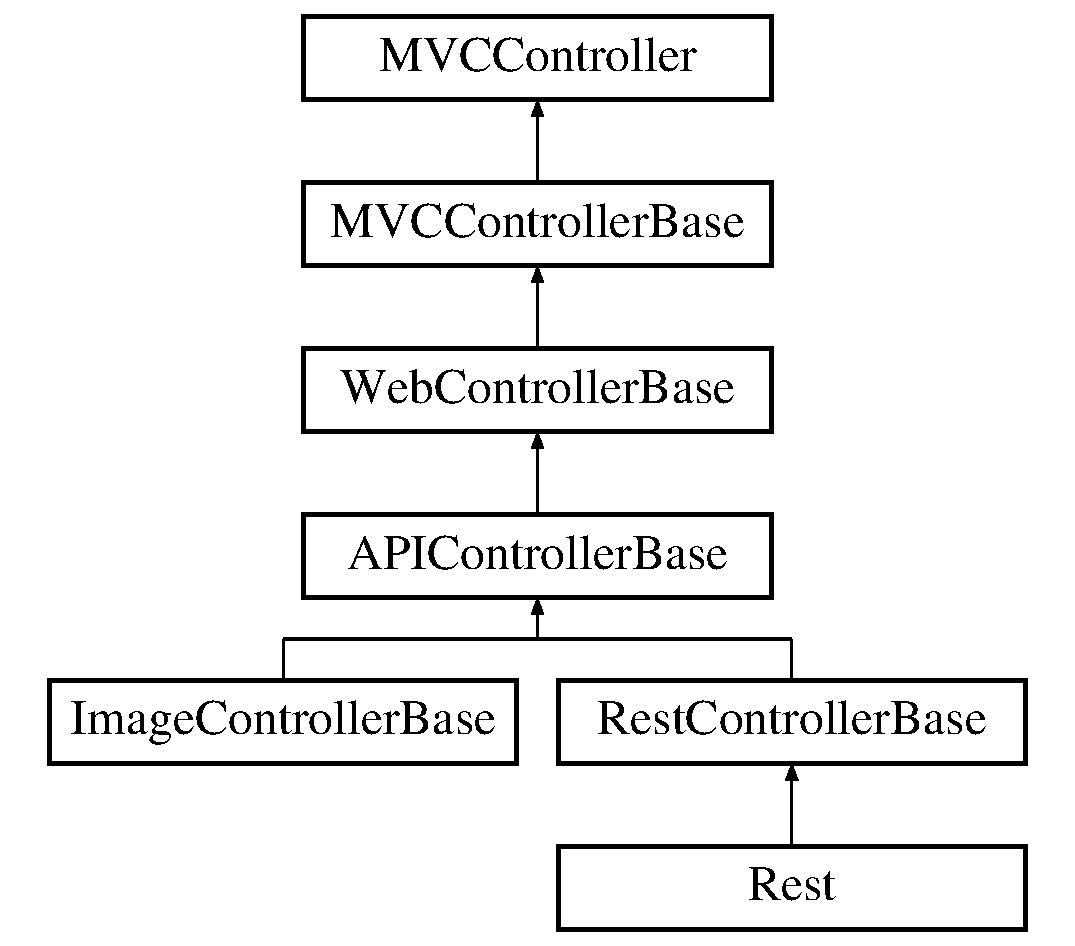
\includegraphics[height=6.000000cm]{class_a_p_i_controller_base}
\end{center}
\end{figure}
\subsection*{公開変数類}
\begin{DoxyCompactItemize}
\item 
\hypertarget{class_a_p_i_controller_base_abc0ec09daf4e9e08caa4a4ad9af5fa7b}{}{\bfseries \$http\+Status} = 200\label{class_a_p_i_controller_base_abc0ec09daf4e9e08caa4a4ad9af5fa7b}

\item 
\hypertarget{class_a_p_i_controller_base_ae31a17a759527251f174a7874c05fe4a}{}{\bfseries \$output\+Type} = \char`\"{}json\char`\"{}\label{class_a_p_i_controller_base_ae31a17a759527251f174a7874c05fe4a}

\item 
\hypertarget{class_a_p_i_controller_base_a938a02e1bd646e49dcb898e61878551c}{}{\bfseries \$validate\+Error} = \char`\"{}\char`\"{}\label{class_a_p_i_controller_base_a938a02e1bd646e49dcb898e61878551c}

\item 
\hypertarget{class_a_p_i_controller_base_ad327eff759e71d160c6b950a50253675}{}{\bfseries \$json\+Unescaped\+Unicode} = true\label{class_a_p_i_controller_base_ad327eff759e71d160c6b950a50253675}

\end{DoxyCompactItemize}
\subsection*{静的限定公開メンバ関数}
\begin{DoxyCompactItemize}
\item 
\hypertarget{class_a_p_i_controller_base_af4481a33cc0b486ed1853937902e13aa}{}static {\bfseries \+\_\+clear\+Cache\+Image} (\$arg\+File\+Path, \$arg\+Memcache\+D\+S\+N=N\+U\+L\+L)\label{class_a_p_i_controller_base_af4481a33cc0b486ed1853937902e13aa}

\end{DoxyCompactItemize}
\subsection*{その他の継承メンバ}


このクラス詳解は次のファイルから抽出されました\+:\begin{DoxyCompactItemize}
\item 
Framework\+Package/class/\+M\+V\+C/A\+P\+I\+Controller\+Base.\+class.\+php\end{DoxyCompactItemize}

\hypertarget{class_app_migration_manager}{}\section{App\+Migration\+Manager クラス}
\label{class_app_migration_manager}\index{App\+Migration\+Manager@{App\+Migration\+Manager}}
\subsection*{静的公開メンバ関数}
\begin{DoxyCompactItemize}
\item 
\hypertarget{class_app_migration_manager_a89d31f9c8565b07f429587531a4d08ad}{}static {\bfseries generate\+Model} (\$arg\+D\+B\+O, \$arg\+Tbl\+Name, \$arg\+Target\+Project\+Name=N\+U\+L\+L, \$arg\+Target\+Platform=N\+U\+L\+L)\label{class_app_migration_manager_a89d31f9c8565b07f429587531a4d08ad}

\end{DoxyCompactItemize}


このクラス詳解は次のファイルから抽出されました\+:\begin{DoxyCompactItemize}
\item 
Framework\+Package/class/\+Smartphone/App\+Migration\+Manager.\+class.\+php\end{DoxyCompactItemize}

\hypertarget{class_auth}{}\section{Auth クラス}
\label{class_auth}\index{Auth@{Auth}}
\subsection*{静的公開メンバ関数}
\begin{DoxyCompactItemize}
\item 
\hypertarget{class_auth_a0d90d23edfa677120d1d679e6b2d4d0a}{}static {\bfseries init} (\$arg\+D\+S\+N=N\+U\+L\+L)\label{class_auth_a0d90d23edfa677120d1d679e6b2d4d0a}

\item 
\hypertarget{class_auth_a1c796b91ca73fbc3711da1c1cbee20fb}{}static {\bfseries get\+Encrypted\+Auth\+Identifier} (\$arg\+Identifier=N\+U\+L\+L)\label{class_auth_a1c796b91ca73fbc3711da1c1cbee20fb}

\item 
\hypertarget{class_auth_a30b9301ad9e08ed19f8998aa1ae7e2eb}{}static {\bfseries get\+Decrypted\+Auth\+Identifier} (\$arg\+Identifier=N\+U\+L\+L)\label{class_auth_a30b9301ad9e08ed19f8998aa1ae7e2eb}

\item 
static \hyperlink{class_auth_a39a95cdcc33ebdfe6d9fa0b1ed7a8105}{get\+Certified\+User} (\$arg\+D\+S\+N=N\+U\+L\+L)
\item 
static \hyperlink{class_auth_a41a4a347f32312fd8080a0098d3559e8}{is\+Certification} (\$arg\+D\+S\+N=N\+U\+L\+L)
\item 
static \hyperlink{class_auth_af19cda27bb71cd0f02c6eedc5d77fd5b}{certify} (\$arg\+I\+D=N\+U\+L\+L, \$arg\+Pass=N\+U\+L\+L, \$arg\+D\+S\+N=N\+U\+L\+L, \$arg\+Execut=F\+A\+L\+S\+E)
\item 
static \hyperlink{class_auth_a35214c906d67d5291aedc6ae3077a306}{un\+Certify} (\$arg\+D\+S\+N=N\+U\+L\+L)
\item 
static \hyperlink{class_auth_a239cdd7ce4421378ed50c4ee13497ec6}{get\+Registered\+User} (\$arg\+I\+D=N\+U\+L\+L, \$arg\+Pass=N\+U\+L\+L, \$arg\+D\+S\+N=N\+U\+L\+L)
\item 
static \hyperlink{class_auth_ad8e06958d26cd1033330eb0c0dcf8237}{is\+Registered} (\$arg\+I\+D=N\+U\+L\+L, \$arg\+Pass=N\+U\+L\+L, \$arg\+D\+S\+N=N\+U\+L\+L)
\item 
static \hyperlink{class_auth_adb637e94fe36d671e36571f1b44bc89c}{registration} (\$arg\+I\+D=N\+U\+L\+L, \$arg\+Pass=N\+U\+L\+L, \$arg\+Date=N\+U\+L\+L, \$arg\+D\+S\+N=N\+U\+L\+L)
\end{DoxyCompactItemize}
\subsection*{静的公開変数類}
\begin{DoxyCompactItemize}
\item 
\hypertarget{class_auth_a03a809bbbfc02f20d510efa62f63ba5c}{}static {\bfseries \$auth\+Table} = \textquotesingle{}user\+\_\+table\textquotesingle{}\label{class_auth_a03a809bbbfc02f20d510efa62f63ba5c}

\item 
\hypertarget{class_auth_a5b7fb197d46cae1d222e6507a28f8273}{}static {\bfseries \$auth\+P\+Key\+Field} = \textquotesingle{}id\textquotesingle{}\label{class_auth_a5b7fb197d46cae1d222e6507a28f8273}

\item 
\hypertarget{class_auth_a1a1e9c62415af1e3be9d2e553cdbad25}{}static {\bfseries \$auth\+I\+D\+Field} = \textquotesingle{}mailaddress\textquotesingle{}\label{class_auth_a1a1e9c62415af1e3be9d2e553cdbad25}

\item 
\hypertarget{class_auth_ab253bd6a9a2bc5b8506a70aee6d66966}{}static {\bfseries \$auth\+Pass\+Field} = \textquotesingle{}password\textquotesingle{}\label{class_auth_ab253bd6a9a2bc5b8506a70aee6d66966}

\item 
\hypertarget{class_auth_af3a21942b3b0e75ff8f3aef25f4ba4ea}{}static {\bfseries \$auth\+Created\+Field} = \textquotesingle{}create\+\_\+date\textquotesingle{}\label{class_auth_af3a21942b3b0e75ff8f3aef25f4ba4ea}

\item 
\hypertarget{class_auth_aec98f90d8d9b9249e867bc37982b3b17}{}static {\bfseries \$auth\+Modified\+Field} = \textquotesingle{}modify\+\_\+date\textquotesingle{}\label{class_auth_aec98f90d8d9b9249e867bc37982b3b17}

\item 
\hypertarget{class_auth_aeb9548ba124de21158de2d51eae93221}{}static {\bfseries \$auth\+I\+D\+Encrypted} = \textquotesingle{}A\+E\+S128\+C\+B\+C\textquotesingle{}\label{class_auth_aeb9548ba124de21158de2d51eae93221}

\item 
\hypertarget{class_auth_a585e0969b2397e80a1bba246a1aee2a1}{}static {\bfseries \$auth\+Pass\+Encrypted} = \textquotesingle{}S\+H\+A256\textquotesingle{}\label{class_auth_a585e0969b2397e80a1bba246a1aee2a1}

\end{DoxyCompactItemize}
\subsection*{静的限定公開メンバ関数}
\begin{DoxyCompactItemize}
\item 
\hypertarget{class_auth_ac59ef46d51ed400b343c9ececd308e24}{}static {\bfseries \+\_\+init} (\$arg\+D\+S\+N=N\+U\+L\+L)\label{class_auth_ac59ef46d51ed400b343c9ececd308e24}

\item 
static \hyperlink{class_auth_a8530363c699c10036e8317881419a9d0}{\+\_\+resolve\+Encrypted} (\$arg\+String, \$arg\+Algorism=N\+U\+L\+L)
\end{DoxyCompactItemize}
\subsection*{静的限定公開変数類}
\begin{DoxyCompactItemize}
\item 
\hypertarget{class_auth_a565d83dd2380d91ffa5f12d62dc5a4de}{}static {\bfseries \$\+\_\+session\+Crypt\+Key} = N\+U\+L\+L\label{class_auth_a565d83dd2380d91ffa5f12d62dc5a4de}

\item 
\hypertarget{class_auth_a65a0bf879f0557085e49a43ae490f1a2}{}static {\bfseries \$\+\_\+session\+Crypt\+I\+V} = N\+U\+L\+L\label{class_auth_a65a0bf879f0557085e49a43ae490f1a2}

\item 
\hypertarget{class_auth_af7ecc71fc76b007ffcf44f4f6e75c51a}{}static {\bfseries \$\+\_\+auth\+Crypt\+Key} = N\+U\+L\+L\label{class_auth_af7ecc71fc76b007ffcf44f4f6e75c51a}

\item 
\hypertarget{class_auth_a6fd50a3bc1beb343064ae57c416f4baf}{}static {\bfseries \$\+\_\+auth\+Crypt\+I\+V} = N\+U\+L\+L\label{class_auth_a6fd50a3bc1beb343064ae57c416f4baf}

\item 
\hypertarget{class_auth_a02b83cf2ecb5cfc5b9195d364467a784}{}static {\bfseries \$\+\_\+\+D\+B\+O} = N\+U\+L\+L\label{class_auth_a02b83cf2ecb5cfc5b9195d364467a784}

\item 
\hypertarget{class_auth_a4c9c442e597e0f35f4b7bd60f981ce54}{}static {\bfseries \$\+\_\+initialized} = F\+A\+L\+S\+E\label{class_auth_a4c9c442e597e0f35f4b7bd60f981ce54}

\end{DoxyCompactItemize}


\subsection{関数詳解}
\hypertarget{class_auth_a8530363c699c10036e8317881419a9d0}{}\index{Auth@{Auth}!\+\_\+resolve\+Encrypted@{\+\_\+resolve\+Encrypted}}
\index{\+\_\+resolve\+Encrypted@{\+\_\+resolve\+Encrypted}!Auth@{Auth}}
\subsubsection[{\+\_\+resolve\+Encrypted}]{\setlength{\rightskip}{0pt plus 5cm}static Auth\+::\+\_\+resolve\+Encrypted (
\begin{DoxyParamCaption}
\item[{}]{\$arg\+String, }
\item[{}]{\$arg\+Algorism = {\ttfamily NULL}}
\end{DoxyParamCaption}
)\hspace{0.3cm}{\ttfamily [static]}, {\ttfamily [protected]}}\label{class_auth_a8530363c699c10036e8317881419a9d0}
登録済みかどうか 
\begin{DoxyParams}[1]{引数}
string & {\em \$arg\+D\+S\+N} & \\
\hline
\end{DoxyParams}
\hypertarget{class_auth_af19cda27bb71cd0f02c6eedc5d77fd5b}{}\index{Auth@{Auth}!certify@{certify}}
\index{certify@{certify}!Auth@{Auth}}
\subsubsection[{certify}]{\setlength{\rightskip}{0pt plus 5cm}static Auth\+::certify (
\begin{DoxyParamCaption}
\item[{}]{\$arg\+I\+D = {\ttfamily NULL}, }
\item[{}]{\$arg\+Pass = {\ttfamily NULL}, }
\item[{}]{\$arg\+D\+S\+N = {\ttfamily NULL}, }
\item[{}]{\$arg\+Execut = {\ttfamily FALSE}}
\end{DoxyParamCaption}
)\hspace{0.3cm}{\ttfamily [static]}}\label{class_auth_af19cda27bb71cd0f02c6eedc5d77fd5b}
認証を証明する(ログインしてセッションを発行する) 
\begin{DoxyParams}{引数}
{\em string} & 認証\+I\+D \\
\hline
{\em string} & 認証パスワード \\
\hline
{\em string} & D\+B接続情報 \\
\hline
{\em string} & 強制再認証 \\
\hline
\end{DoxyParams}
\hypertarget{class_auth_a39a95cdcc33ebdfe6d9fa0b1ed7a8105}{}\index{Auth@{Auth}!get\+Certified\+User@{get\+Certified\+User}}
\index{get\+Certified\+User@{get\+Certified\+User}!Auth@{Auth}}
\subsubsection[{get\+Certified\+User}]{\setlength{\rightskip}{0pt plus 5cm}static Auth\+::get\+Certified\+User (
\begin{DoxyParamCaption}
\item[{}]{\$arg\+D\+S\+N = {\ttfamily NULL}}
\end{DoxyParamCaption}
)\hspace{0.3cm}{\ttfamily [static]}}\label{class_auth_a39a95cdcc33ebdfe6d9fa0b1ed7a8105}
認証が証明済みのユーザーモデルを返す 
\begin{DoxyParams}{引数}
{\em string} & D\+B接続情報 \\
\hline
\end{DoxyParams}
\hypertarget{class_auth_a239cdd7ce4421378ed50c4ee13497ec6}{}\index{Auth@{Auth}!get\+Registered\+User@{get\+Registered\+User}}
\index{get\+Registered\+User@{get\+Registered\+User}!Auth@{Auth}}
\subsubsection[{get\+Registered\+User}]{\setlength{\rightskip}{0pt plus 5cm}static Auth\+::get\+Registered\+User (
\begin{DoxyParamCaption}
\item[{}]{\$arg\+I\+D = {\ttfamily NULL}, }
\item[{}]{\$arg\+Pass = {\ttfamily NULL}, }
\item[{}]{\$arg\+D\+S\+N = {\ttfamily NULL}}
\end{DoxyParamCaption}
)\hspace{0.3cm}{\ttfamily [static]}}\label{class_auth_a239cdd7ce4421378ed50c4ee13497ec6}
登録済みかどうか 
\begin{DoxyParams}[1]{引数}
string & {\em \$arg\+D\+S\+N} & \\
\hline
\end{DoxyParams}
\hypertarget{class_auth_a41a4a347f32312fd8080a0098d3559e8}{}\index{Auth@{Auth}!is\+Certification@{is\+Certification}}
\index{is\+Certification@{is\+Certification}!Auth@{Auth}}
\subsubsection[{is\+Certification}]{\setlength{\rightskip}{0pt plus 5cm}static Auth\+::is\+Certification (
\begin{DoxyParamCaption}
\item[{}]{\$arg\+D\+S\+N = {\ttfamily NULL}}
\end{DoxyParamCaption}
)\hspace{0.3cm}{\ttfamily [static]}}\label{class_auth_a41a4a347f32312fd8080a0098d3559e8}
認証が証明済みかどうか(セッションが既にあるかどうか) 
\begin{DoxyParams}{引数}
{\em string} & D\+B接続情報 \\
\hline
\end{DoxyParams}
\hypertarget{class_auth_ad8e06958d26cd1033330eb0c0dcf8237}{}\index{Auth@{Auth}!is\+Registered@{is\+Registered}}
\index{is\+Registered@{is\+Registered}!Auth@{Auth}}
\subsubsection[{is\+Registered}]{\setlength{\rightskip}{0pt plus 5cm}static Auth\+::is\+Registered (
\begin{DoxyParamCaption}
\item[{}]{\$arg\+I\+D = {\ttfamily NULL}, }
\item[{}]{\$arg\+Pass = {\ttfamily NULL}, }
\item[{}]{\$arg\+D\+S\+N = {\ttfamily NULL}}
\end{DoxyParamCaption}
)\hspace{0.3cm}{\ttfamily [static]}}\label{class_auth_ad8e06958d26cd1033330eb0c0dcf8237}
登録済みかどうか 
\begin{DoxyParams}[1]{引数}
string & {\em \$arg\+D\+S\+N} & \\
\hline
\end{DoxyParams}
\hypertarget{class_auth_adb637e94fe36d671e36571f1b44bc89c}{}\index{Auth@{Auth}!registration@{registration}}
\index{registration@{registration}!Auth@{Auth}}
\subsubsection[{registration}]{\setlength{\rightskip}{0pt plus 5cm}static Auth\+::registration (
\begin{DoxyParamCaption}
\item[{}]{\$arg\+I\+D = {\ttfamily NULL}, }
\item[{}]{\$arg\+Pass = {\ttfamily NULL}, }
\item[{}]{\$arg\+Date = {\ttfamily NULL}, }
\item[{}]{\$arg\+D\+S\+N = {\ttfamily NULL}}
\end{DoxyParamCaption}
)\hspace{0.3cm}{\ttfamily [static]}}\label{class_auth_adb637e94fe36d671e36571f1b44bc89c}
登録する 
\begin{DoxyParams}{引数}
{\em string} & D\+B接続情報 \\
\hline
\end{DoxyParams}
\hypertarget{class_auth_a35214c906d67d5291aedc6ae3077a306}{}\index{Auth@{Auth}!un\+Certify@{un\+Certify}}
\index{un\+Certify@{un\+Certify}!Auth@{Auth}}
\subsubsection[{un\+Certify}]{\setlength{\rightskip}{0pt plus 5cm}static Auth\+::un\+Certify (
\begin{DoxyParamCaption}
\item[{}]{\$arg\+D\+S\+N = {\ttfamily NULL}}
\end{DoxyParamCaption}
)\hspace{0.3cm}{\ttfamily [static]}}\label{class_auth_a35214c906d67d5291aedc6ae3077a306}
認証を非証明する(ログアウトする) 
\begin{DoxyParams}{引数}
{\em string} & D\+B接続情報 \\
\hline
\end{DoxyParams}


このクラス詳解は次のファイルから抽出されました\+:\begin{DoxyCompactItemize}
\item 
Framework\+Package/class/\+Auth/Auth.\+class.\+php\end{DoxyCompactItemize}

\hypertarget{class_base_append_filter}{}\section{Base\+Append\+Filter クラス}
\label{class_base_append_filter}\index{Base\+Append\+Filter@{Base\+Append\+Filter}}
\subsection*{公開メンバ関数}
\begin{DoxyCompactItemize}
\item 
\hypertarget{class_base_append_filter_a670b60ec4105736d8f64d1b6f28b2b16}{}{\bfseries execute} ()\label{class_base_append_filter_a670b60ec4105736d8f64d1b6f28b2b16}

\end{DoxyCompactItemize}


このクラス詳解は次のファイルから抽出されました\+:\begin{DoxyCompactItemize}
\item 
Framework\+Package/class/\+M\+V\+C/\+Controller/\+Filter/Base\+Append\+Filter.\+php\end{DoxyCompactItemize}

\hypertarget{class_base_prepend_filter}{}\section{Base\+Prepend\+Filter クラス}
\label{class_base_prepend_filter}\index{Base\+Prepend\+Filter@{Base\+Prepend\+Filter}}
\subsection*{公開メンバ関数}
\begin{DoxyCompactItemize}
\item 
\hypertarget{class_base_prepend_filter_a8c915ee4ade472f815ef705305db3144}{}{\bfseries execute} (\$arg\+Request\+Params=N\+U\+L\+L)\label{class_base_prepend_filter_a8c915ee4ade472f815ef705305db3144}

\end{DoxyCompactItemize}


\subsection{詳解}
フィルター \begin{DoxyAuthor}{著者}
saimushi 
\end{DoxyAuthor}


このクラス詳解は次のファイルから抽出されました\+:\begin{DoxyCompactItemize}
\item 
Framework\+Package/class/\+M\+V\+C/\+Controller/\+Filter/Base\+Prepend\+Filter.\+php\end{DoxyCompactItemize}

\hypertarget{class_cipher}{}\section{Cipher クラス}
\label{class_cipher}\index{Cipher@{Cipher}}
\subsection*{公開メンバ関数}
\begin{DoxyCompactItemize}
\item 
\hyperlink{class_cipher_a35e01f22996f07ab76a98e43901ce16d}{\+\_\+\+\_\+construct} ()
\item 
\hyperlink{class_cipher_a98a6560d7d2636194b0ba4a3335a2d41}{\+\_\+\+\_\+destruct} ()
\end{DoxyCompactItemize}
\subsection*{静的公開メンバ関数}
\begin{DoxyCompactItemize}
\item 
static \hyperlink{class_cipher_af83586f4fa8657c1c92b74a576cf454b}{encrypt} (\$arguments)
\item 
static \hyperlink{class_cipher_a0f4e2a0af5e67c1d66446301b367c4e1}{decrypt} (\$arguments)
\item 
static \hyperlink{class_cipher_adab7e1a9d0f7ef9ef956647383dfb8ab}{get\+Now\+I\+V} ()
\item 
static \hyperlink{class_cipher_a1985ff8212d2cda46bdf516e2e3e413f}{pad} (\$text, \$blocksize)
\item 
static \hyperlink{class_cipher_a1ddce1e31a41e331de65541c00436ac8}{unpad} (\$text)
\end{DoxyCompactItemize}
\subsection*{静的限定公開変数類}
\begin{DoxyCompactItemize}
\item 
\hypertarget{class_cipher_a8f76dc59d62626a82553636606ec3e98}{}static {\bfseries \$iv} = N\+U\+L\+L\label{class_cipher_a8f76dc59d62626a82553636606ec3e98}

\end{DoxyCompactItemize}


\subsection{詳解}
暗号化処理を行います。

ブロックアルゴリズムをサポートするmcryptライブラリを利用しています。 \begin{DoxyAuthor}{著者}
T.\+Morita 
\end{DoxyAuthor}
\begin{DoxySeeAlso}{参照}
\href{http://php.net/manual/ja/book.mcrypt.php}{\tt Mcrypt} 
\end{DoxySeeAlso}


\subsection{構築子と解体子}
\hypertarget{class_cipher_a35e01f22996f07ab76a98e43901ce16d}{}\index{Cipher@{Cipher}!\+\_\+\+\_\+construct@{\+\_\+\+\_\+construct}}
\index{\+\_\+\+\_\+construct@{\+\_\+\+\_\+construct}!Cipher@{Cipher}}
\subsubsection[{\+\_\+\+\_\+construct}]{\setlength{\rightskip}{0pt plus 5cm}Cipher\+::\+\_\+\+\_\+construct (
\begin{DoxyParamCaption}
{}
\end{DoxyParamCaption}
)}\label{class_cipher_a35e01f22996f07ab76a98e43901ce16d}
コンストラクタ \hypertarget{class_cipher_a98a6560d7d2636194b0ba4a3335a2d41}{}\index{Cipher@{Cipher}!\+\_\+\+\_\+destruct@{\+\_\+\+\_\+destruct}}
\index{\+\_\+\+\_\+destruct@{\+\_\+\+\_\+destruct}!Cipher@{Cipher}}
\subsubsection[{\+\_\+\+\_\+destruct}]{\setlength{\rightskip}{0pt plus 5cm}Cipher\+::\+\_\+\+\_\+destruct (
\begin{DoxyParamCaption}
{}
\end{DoxyParamCaption}
)}\label{class_cipher_a98a6560d7d2636194b0ba4a3335a2d41}
デストラクタ 

\subsection{関数詳解}
\hypertarget{class_cipher_a0f4e2a0af5e67c1d66446301b367c4e1}{}\index{Cipher@{Cipher}!decrypt@{decrypt}}
\index{decrypt@{decrypt}!Cipher@{Cipher}}
\subsubsection[{decrypt}]{\setlength{\rightskip}{0pt plus 5cm}static Cipher\+::decrypt (
\begin{DoxyParamCaption}
\item[{}]{\$arguments}
\end{DoxyParamCaption}
)\hspace{0.3cm}{\ttfamily [static]}}\label{class_cipher_a0f4e2a0af5e67c1d66446301b367c4e1}
データを復号化する 
\begin{DoxyParams}[1]{引数}
array & {\em \$arguments} & 復号情報 \begin{TabularNC}{5}
\hline
{\bfseries key} &{\bfseries type} &{\bfseries require} &{\bfseries default} &{\bfseries description}  \\\cline{1-5}
value &string &true &&対象データ  \\\cline{1-5}
key &string &true &&暗号キー  \\\cline{1-5}
iv &string &false &指定されない場合生成される &初期化ベクトル  \\\cline{1-5}
algorithm &string &false &rijndael-\/128 &M\+C\+R\+Y\+P\+T\+\_\+暗号名 定数のいずれか、 あるいはアルゴリズム名をあらわす文字列。  \\\cline{1-5}
mode &string &false &cbc &定数 M\+C\+R\+Y\+P\+T\+\_\+\+M\+O\+D\+E\+\_\+モード名、あるいは文字列 \char`\"{}ecb\char`\"{}, \char`\"{}cbc\char`\"{}, \char`\"{}cfb\char`\"{}, \char`\"{}ofb\char`\"{}, \char`\"{}nofb\char`\"{} ,\char`\"{}stream\char`\"{} のいずれか。  \\\cline{1-5}
prefix &string &false&&接頭にパディングする文字列  \\\cline{1-5}
suffix &string &false &&接尾にパディングする文字列  \\\cline{1-5}
\end{TabularNC}
パディング防止が必要な場合は、\textquotesingle{}prefix\textquotesingle{}と\textquotesingle{}suffix\textquotesingle{}を指定する。~\newline
 \textquotesingle{}prefix\textquotesingle{}と\textquotesingle{}suffix\textquotesingle{}には、メタ文字( . \textbackslash{} + $\ast$ ? \mbox{[} $^\wedge$ \mbox{]} ( \$ ) )のみ指定できます。 \\
\hline
\end{DoxyParams}
\begin{DoxyReturn}{戻り値}
string$\vert$boolean 復号化されたデータもしくはfalse 
\end{DoxyReturn}
\hypertarget{class_cipher_af83586f4fa8657c1c92b74a576cf454b}{}\index{Cipher@{Cipher}!encrypt@{encrypt}}
\index{encrypt@{encrypt}!Cipher@{Cipher}}
\subsubsection[{encrypt}]{\setlength{\rightskip}{0pt plus 5cm}static Cipher\+::encrypt (
\begin{DoxyParamCaption}
\item[{}]{\$arguments}
\end{DoxyParamCaption}
)\hspace{0.3cm}{\ttfamily [static]}}\label{class_cipher_af83586f4fa8657c1c92b74a576cf454b}
データを暗号化する 
\begin{DoxyParams}[1]{引数}
array & {\em \$arguments} & 暗号情報 \begin{TabularNC}{5}
\hline
{\bfseries key} &{\bfseries type} &{\bfseries require} &{\bfseries default} &{\bfseries description}  \\\cline{1-5}
value &string &true &&対象データ  \\\cline{1-5}
key &string &true &&暗号キー  \\\cline{1-5}
iv &string &false &指定されない場合生成される &初期化ベクトル  \\\cline{1-5}
algorithm &string &false &rijndael-\/128 &M\+C\+R\+Y\+P\+T\+\_\+暗号名 定数のいずれか、 あるいはアルゴリズム名をあらわす文字列。  \\\cline{1-5}
mode &string &false &cbc &定数 M\+C\+R\+Y\+P\+T\+\_\+\+M\+O\+D\+E\+\_\+モード名、あるいは文字列 \char`\"{}ecb\char`\"{}, \char`\"{}cbc\char`\"{}, \char`\"{}cfb\char`\"{}, \char`\"{}ofb\char`\"{}, \char`\"{}nofb\char`\"{} ,\char`\"{}stream\char`\"{} のいずれか。  \\\cline{1-5}
prefix &string &false&&接頭にパディングする文字列  \\\cline{1-5}
suffix &string &false &&接尾にパディングする文字列  \\\cline{1-5}
\end{TabularNC}
パディング防止が必要な場合は、\textquotesingle{}prefix\textquotesingle{}と\textquotesingle{}suffix\textquotesingle{}を指定する。~\newline
 \textquotesingle{}prefix\textquotesingle{}と\textquotesingle{}suffix\textquotesingle{}には、メタ文字( . \textbackslash{} + $\ast$ ? \mbox{[} $^\wedge$ \mbox{]} ( \$ ) )のみ指定できます。 \\
\hline
\end{DoxyParams}
\begin{DoxyReturn}{戻り値}
string$\vert$boolean 暗号化されたデータもしくはfalse 
\end{DoxyReturn}
\hypertarget{class_cipher_adab7e1a9d0f7ef9ef956647383dfb8ab}{}\index{Cipher@{Cipher}!get\+Now\+I\+V@{get\+Now\+I\+V}}
\index{get\+Now\+I\+V@{get\+Now\+I\+V}!Cipher@{Cipher}}
\subsubsection[{get\+Now\+I\+V}]{\setlength{\rightskip}{0pt plus 5cm}static Cipher\+::get\+Now\+I\+V (
\begin{DoxyParamCaption}
{}
\end{DoxyParamCaption}
)\hspace{0.3cm}{\ttfamily [static]}}\label{class_cipher_adab7e1a9d0f7ef9ef956647383dfb8ab}
現在設定されている、最後に使用された\+I\+V(初期化ベクトル)を返す \begin{DoxyReturn}{戻り値}
string 初期化ベクトル 
\end{DoxyReturn}
\hypertarget{class_cipher_a1985ff8212d2cda46bdf516e2e3e413f}{}\index{Cipher@{Cipher}!pad@{pad}}
\index{pad@{pad}!Cipher@{Cipher}}
\subsubsection[{pad}]{\setlength{\rightskip}{0pt plus 5cm}static Cipher\+::pad (
\begin{DoxyParamCaption}
\item[{}]{\$text, }
\item[{}]{\$blocksize}
\end{DoxyParamCaption}
)\hspace{0.3cm}{\ttfamily [static]}}\label{class_cipher_a1985ff8212d2cda46bdf516e2e3e413f}
P\+K\+C\+Sでpadする(5、7に有効) 
\begin{DoxyParams}[1]{引数}
string & {\em \$text} & 対象文字列 \\
\hline
integer & {\em \$blocksize} & ブロックサイズ \\
\hline
\end{DoxyParams}
\begin{DoxyReturn}{戻り値}
string padされた文字列 
\end{DoxyReturn}
\begin{DoxySeeAlso}{参照}
\href{http://ja.wikipedia.org/wiki/PKCS}{\tt P\+K\+C\+S} 
\end{DoxySeeAlso}
\hypertarget{class_cipher_a1ddce1e31a41e331de65541c00436ac8}{}\index{Cipher@{Cipher}!unpad@{unpad}}
\index{unpad@{unpad}!Cipher@{Cipher}}
\subsubsection[{unpad}]{\setlength{\rightskip}{0pt plus 5cm}static Cipher\+::unpad (
\begin{DoxyParamCaption}
\item[{}]{\$text}
\end{DoxyParamCaption}
)\hspace{0.3cm}{\ttfamily [static]}}\label{class_cipher_a1ddce1e31a41e331de65541c00436ac8}
P\+K\+C\+Sでunpadする(5、7に有効) 
\begin{DoxyParams}[1]{引数}
string & {\em \$text} & 対象文字列 \\
\hline
\end{DoxyParams}
\begin{DoxyReturn}{戻り値}
string unpadされた文字列 
\end{DoxyReturn}
\begin{DoxySeeAlso}{参照}
\href{http://ja.wikipedia.org/wiki/PKCS}{\tt P\+K\+C\+S} 
\end{DoxySeeAlso}


このクラス詳解は次のファイルから抽出されました\+:\begin{DoxyCompactItemize}
\item 
Generic\+Package/class/\+Cipher/Cipher.\+class.\+php\end{DoxyCompactItemize}

\hypertarget{class_d_e_s}{}\section{D\+E\+S クラス}
\label{class_d_e_s}\index{D\+E\+S@{D\+E\+S}}
\subsection*{公開メンバ関数}
\begin{DoxyCompactItemize}
\item 
\hyperlink{class_d_e_s_a845dd4f82f378af191af6d5a48779e4d}{encrypt} (\$message, \$key)
\item 
\hyperlink{class_d_e_s_af388fb06ed6f9fd4e7578cc5eb908a0f}{decrypt} (\$message, \$key)
\item 
\hyperlink{class_d_e_s_ace44dc8314b69a7b34cac8325c0a4820}{execute} (\$key, \$message, \$\hyperlink{class_d_e_s_a845dd4f82f378af191af6d5a48779e4d}{encrypt}, \$mode, \$iv, \$padding=2)
\end{DoxyCompactItemize}


\subsection{関数詳解}
\hypertarget{class_d_e_s_af388fb06ed6f9fd4e7578cc5eb908a0f}{}\index{D\+E\+S@{D\+E\+S}!decrypt@{decrypt}}
\index{decrypt@{decrypt}!D\+E\+S@{D\+E\+S}}
\subsubsection[{decrypt}]{\setlength{\rightskip}{0pt plus 5cm}D\+E\+S\+::decrypt (
\begin{DoxyParamCaption}
\item[{}]{\$message, }
\item[{}]{\$key}
\end{DoxyParamCaption}
)}\label{class_d_e_s_af388fb06ed6f9fd4e7578cc5eb908a0f}
複合化 \begin{DoxyReturn}{戻り値}

\end{DoxyReturn}

\begin{DoxyParams}[1]{引数}
object & {\em \$key} & \\
\hline
object & {\em \$message} & \\
\hline
\end{DoxyParams}
\hypertarget{class_d_e_s_a845dd4f82f378af191af6d5a48779e4d}{}\index{D\+E\+S@{D\+E\+S}!encrypt@{encrypt}}
\index{encrypt@{encrypt}!D\+E\+S@{D\+E\+S}}
\subsubsection[{encrypt}]{\setlength{\rightskip}{0pt plus 5cm}D\+E\+S\+::encrypt (
\begin{DoxyParamCaption}
\item[{}]{\$message, }
\item[{}]{\$key}
\end{DoxyParamCaption}
)}\label{class_d_e_s_a845dd4f82f378af191af6d5a48779e4d}
暗号化 \begin{DoxyReturn}{戻り値}

\end{DoxyReturn}

\begin{DoxyParams}[1]{引数}
object & {\em \$key} & \\
\hline
object & {\em \$message} & \\
\hline
\end{DoxyParams}
\hypertarget{class_d_e_s_ace44dc8314b69a7b34cac8325c0a4820}{}\index{D\+E\+S@{D\+E\+S}!execute@{execute}}
\index{execute@{execute}!D\+E\+S@{D\+E\+S}}
\subsubsection[{execute}]{\setlength{\rightskip}{0pt plus 5cm}D\+E\+S\+::execute (
\begin{DoxyParamCaption}
\item[{}]{\$key, }
\item[{}]{\$message, }
\item[{}]{\$encrypt, }
\item[{}]{\$mode, }
\item[{}]{\$iv, }
\item[{}]{\$padding = {\ttfamily 2}}
\end{DoxyParamCaption}
)}\label{class_d_e_s_ace44dc8314b69a7b34cac8325c0a4820}
renamed to des\+\_\+des so php doesn\textquotesingle{}t use it as a constructor \begin{DoxyReturn}{戻り値}

\end{DoxyReturn}

\begin{DoxyParams}[1]{引数}
object & {\em \$key} & \\
\hline
object & {\em \$message} & \\
\hline
object & {\em \$encrypt} & \\
\hline
object & {\em \$mode} & \\
\hline
object & {\em \$iv} & \\
\hline
object & {\em \$padding,\mbox{[}optional\mbox{]}} & \\
\hline
\end{DoxyParams}


このクラス詳解は次のファイルから抽出されました\+:\begin{DoxyCompactItemize}
\item 
Generic\+Package/function/D\+E\+S.\+inc.\+php\end{DoxyCompactItemize}

\hypertarget{class_flow_manager}{}\section{Flow\+Manager クラス}
\label{class_flow_manager}\index{Flow\+Manager@{Flow\+Manager}}
\subsection*{静的公開メンバ関数}
\begin{DoxyCompactItemize}
\item 
static \hyperlink{class_flow_manager_a6af8cf1d11afa9ba639fc2e2118070b4}{validate} (\$arg\+Container\+X\+M\+L)
\item 
\hypertarget{class_flow_manager_a5d92e9d445a8bf523f7f12e83e68a344}{}static {\bfseries reverse\+Rewrite\+U\+R\+L} (\$arg\+Action, \$arg\+Query=\textquotesingle{}\textquotesingle{})\label{class_flow_manager_a5d92e9d445a8bf523f7f12e83e68a344}

\item 
static \hyperlink{class_flow_manager_aec2bdc919808a821598cfedf427dd6fd}{load\+Next\+Flow} (\$arg\+Class\+Name=N\+U\+L\+L, \$arg\+Target\+Path= \textquotesingle{}\textquotesingle{})
\item 
static \hyperlink{class_flow_manager_a514963c4885f0eaedd17ec5193cf276a}{generate} (\$arg\+Target, \$arg\+Section, \$arg\+Base\+Path\+Target=\textquotesingle{}\textquotesingle{})
\item 
static \hyperlink{class_flow_manager_a3bc3ae3b6b4efea3c010942ca1e2bab7}{\+\_\+get\+Autogenerate\+Target\+Path} (\$arg\+Target)
\item 
static \hyperlink{class_flow_manager_a331069b41a81d00cac4685158ef8f575}{\+\_\+get\+Autogenerate\+File\+Path} (\$arg\+Target)
\item 
static \hyperlink{class_flow_manager_a22727b3f5902ba4d86017f5552e20718}{\+\_\+generate\+Code} (\$arg\+Code\+Node, \$arg\+Base\+Path\+Target=\textquotesingle{}\textquotesingle{}, \$arg\+Depth=1)
\item 
static \hyperlink{class_flow_manager_a32c69da4b4be7d0f0b67b080b4a1bc0d}{\+\_\+resolve\+Args} (\$arg\+Attr)
\item 
static \hyperlink{class_flow_manager_aca9727acaadc1b0bc967bb68ede97d73}{\+\_\+resolve\+Value} (\$arg\+Value)
\end{DoxyCompactItemize}
\subsection*{静的公開変数類}
\begin{DoxyCompactItemize}
\item 
\hypertarget{class_flow_manager_a336fb1b43e5db055c4528f204da29418}{}static {\bfseries \$params} = array(\textquotesingle{}post\textquotesingle{}=$>$N\+U\+L\+L, \textquotesingle{}get\textquotesingle{}=$>$N\+U\+L\+L, \textquotesingle{}request\textquotesingle{}=$>$N\+U\+L\+L, \textquotesingle{}view\textquotesingle{}=$>$N\+U\+L\+L, \textquotesingle{}backflow\textquotesingle{}=$>$N\+U\+L\+L)\label{class_flow_manager_a336fb1b43e5db055c4528f204da29418}

\end{DoxyCompactItemize}


\subsection{関数詳解}
\hypertarget{class_flow_manager_a22727b3f5902ba4d86017f5552e20718}{}\index{Flow\+Manager@{Flow\+Manager}!\+\_\+generate\+Code@{\+\_\+generate\+Code}}
\index{\+\_\+generate\+Code@{\+\_\+generate\+Code}!Flow\+Manager@{Flow\+Manager}}
\subsubsection[{\+\_\+generate\+Code}]{\setlength{\rightskip}{0pt plus 5cm}static Flow\+Manager\+::\+\_\+generate\+Code (
\begin{DoxyParamCaption}
\item[{}]{\$arg\+Code\+Node, }
\item[{}]{\$arg\+Base\+Path\+Target = {\ttfamily \textquotesingle{}\textquotesingle{}}, }
\item[{}]{\$arg\+Depth = {\ttfamily 1}}
\end{DoxyParamCaption}
)\hspace{0.3cm}{\ttfamily [static]}}\label{class_flow_manager_a22727b3f5902ba4d86017f5552e20718}
ノードを処理に分解する 
\begin{DoxyParams}[1]{引数}
unknown & {\em \$arg\+Node} & \\
\hline
\end{DoxyParams}
\hypertarget{class_flow_manager_a331069b41a81d00cac4685158ef8f575}{}\index{Flow\+Manager@{Flow\+Manager}!\+\_\+get\+Autogenerate\+File\+Path@{\+\_\+get\+Autogenerate\+File\+Path}}
\index{\+\_\+get\+Autogenerate\+File\+Path@{\+\_\+get\+Autogenerate\+File\+Path}!Flow\+Manager@{Flow\+Manager}}
\subsubsection[{\+\_\+get\+Autogenerate\+File\+Path}]{\setlength{\rightskip}{0pt plus 5cm}static Flow\+Manager\+::\+\_\+get\+Autogenerate\+File\+Path (
\begin{DoxyParamCaption}
\item[{}]{\$arg\+Target}
\end{DoxyParamCaption}
)\hspace{0.3cm}{\ttfamily [static]}}\label{class_flow_manager_a331069b41a81d00cac4685158ef8f575}
ジェネレートファイルのパスを取得する 
\begin{DoxyParams}[1]{引数}
unknown & {\em \$arg\+Node} & \\
\hline
\end{DoxyParams}
\hypertarget{class_flow_manager_a3bc3ae3b6b4efea3c010942ca1e2bab7}{}\index{Flow\+Manager@{Flow\+Manager}!\+\_\+get\+Autogenerate\+Target\+Path@{\+\_\+get\+Autogenerate\+Target\+Path}}
\index{\+\_\+get\+Autogenerate\+Target\+Path@{\+\_\+get\+Autogenerate\+Target\+Path}!Flow\+Manager@{Flow\+Manager}}
\subsubsection[{\+\_\+get\+Autogenerate\+Target\+Path}]{\setlength{\rightskip}{0pt plus 5cm}static Flow\+Manager\+::\+\_\+get\+Autogenerate\+Target\+Path (
\begin{DoxyParamCaption}
\item[{}]{\$arg\+Target}
\end{DoxyParamCaption}
)\hspace{0.3cm}{\ttfamily [static]}}\label{class_flow_manager_a3bc3ae3b6b4efea3c010942ca1e2bab7}
ジェネレートファイルのターゲットパスを取得する 
\begin{DoxyParams}[1]{引数}
unknown & {\em \$arg\+Node} & \\
\hline
\end{DoxyParams}
\hypertarget{class_flow_manager_a32c69da4b4be7d0f0b67b080b4a1bc0d}{}\index{Flow\+Manager@{Flow\+Manager}!\+\_\+resolve\+Args@{\+\_\+resolve\+Args}}
\index{\+\_\+resolve\+Args@{\+\_\+resolve\+Args}!Flow\+Manager@{Flow\+Manager}}
\subsubsection[{\+\_\+resolve\+Args}]{\setlength{\rightskip}{0pt plus 5cm}static Flow\+Manager\+::\+\_\+resolve\+Args (
\begin{DoxyParamCaption}
\item[{}]{\$arg\+Attr}
\end{DoxyParamCaption}
)\hspace{0.3cm}{\ttfamily [static]}}\label{class_flow_manager_a32c69da4b4be7d0f0b67b080b4a1bc0d}
引数の値の解決処理 
\begin{DoxyParams}[1]{引数}
unknown & {\em \$arg\+Node} & \\
\hline
\end{DoxyParams}
\hypertarget{class_flow_manager_aca9727acaadc1b0bc967bb68ede97d73}{}\index{Flow\+Manager@{Flow\+Manager}!\+\_\+resolve\+Value@{\+\_\+resolve\+Value}}
\index{\+\_\+resolve\+Value@{\+\_\+resolve\+Value}!Flow\+Manager@{Flow\+Manager}}
\subsubsection[{\+\_\+resolve\+Value}]{\setlength{\rightskip}{0pt plus 5cm}static Flow\+Manager\+::\+\_\+resolve\+Value (
\begin{DoxyParamCaption}
\item[{}]{\$arg\+Value}
\end{DoxyParamCaption}
)\hspace{0.3cm}{\ttfamily [static]}}\label{class_flow_manager_aca9727acaadc1b0bc967bb68ede97d73}
属性の値の解決処理 
\begin{DoxyParams}[1]{引数}
unknown & {\em \$arg\+Node} & \\
\hline
\end{DoxyParams}
\hypertarget{class_flow_manager_a514963c4885f0eaedd17ec5193cf276a}{}\index{Flow\+Manager@{Flow\+Manager}!generate@{generate}}
\index{generate@{generate}!Flow\+Manager@{Flow\+Manager}}
\subsubsection[{generate}]{\setlength{\rightskip}{0pt plus 5cm}static Flow\+Manager\+::generate (
\begin{DoxyParamCaption}
\item[{}]{\$arg\+Target, }
\item[{}]{\$arg\+Section, }
\item[{}]{\$arg\+Base\+Path\+Target = {\ttfamily \textquotesingle{}\textquotesingle{}}}
\end{DoxyParamCaption}
)\hspace{0.3cm}{\ttfamily [static]}}\label{class_flow_manager_a514963c4885f0eaedd17ec5193cf276a}
定義情報をチェックする 
\begin{DoxyParams}{引数}
{\em string} & X\+M\+Lファイルのパス文字列 or X\+M\+L文字列 \\
\hline
\end{DoxyParams}
\hypertarget{class_flow_manager_aec2bdc919808a821598cfedf427dd6fd}{}\index{Flow\+Manager@{Flow\+Manager}!load\+Next\+Flow@{load\+Next\+Flow}}
\index{load\+Next\+Flow@{load\+Next\+Flow}!Flow\+Manager@{Flow\+Manager}}
\subsubsection[{load\+Next\+Flow}]{\setlength{\rightskip}{0pt plus 5cm}static Flow\+Manager\+::load\+Next\+Flow (
\begin{DoxyParamCaption}
\item[{}]{\$arg\+Class\+Name = {\ttfamily NULL}, }
\item[{}]{\$arg\+Target\+Path = {\ttfamily \textquotesingle{}\textquotesingle{}}}
\end{DoxyParamCaption}
)\hspace{0.3cm}{\ttfamily [static]}}\label{class_flow_manager_aec2bdc919808a821598cfedf427dd6fd}
次の\+Flowを特定し、ロードし、そのクラス名を返却する 
\begin{DoxyParams}{引数}
{\em string} & クラス名 \\
\hline
{\em string} & ターゲットファイルパスのヒント \\
\hline
\end{DoxyParams}
\begin{DoxyReturn}{戻り値}
mixed 成功時は対象のクラス名 失敗した場合は\+F\+A\+L\+S\+Eを返す 
\end{DoxyReturn}
\hypertarget{class_flow_manager_a6af8cf1d11afa9ba639fc2e2118070b4}{}\index{Flow\+Manager@{Flow\+Manager}!validate@{validate}}
\index{validate@{validate}!Flow\+Manager@{Flow\+Manager}}
\subsubsection[{validate}]{\setlength{\rightskip}{0pt plus 5cm}static Flow\+Manager\+::validate (
\begin{DoxyParamCaption}
\item[{}]{\$arg\+Container\+X\+M\+L}
\end{DoxyParamCaption}
)\hspace{0.3cm}{\ttfamily [static]}}\label{class_flow_manager_a6af8cf1d11afa9ba639fc2e2118070b4}
定義情報をチェックする 
\begin{DoxyParams}[1]{引数}
unknown & {\em \$arg\+Container\+X\+M\+L} & \\
\hline
\end{DoxyParams}


このクラス詳解は次のファイルから抽出されました\+:\begin{DoxyCompactItemize}
\item 
Framework\+Package/class/\+Flow/Flow\+Manager.\+class.\+php\end{DoxyCompactItemize}

\hypertarget{class_generic_app_receipt_verifier}{}\section{Generic\+App\+Receipt\+Verifier クラス}
\label{class_generic_app_receipt_verifier}\index{Generic\+App\+Receipt\+Verifier@{Generic\+App\+Receipt\+Verifier}}
\subsection*{静的公開メンバ関数}
\begin{DoxyCompactItemize}
\item 
static \hyperlink{class_generic_app_receipt_verifier_a388ae0d1c431633edb1a7cce05d4009e}{is\+Enabled} (\$arg\+Product\+I\+D, \$arg\+Base64\+Encoded\+Receipt, \$arg\+Device\+Type, \$arg\+Signature\+Or\+Secret\+Key, \$arg\+Autorenew\+Subscription=F\+A\+L\+S\+E, \$arg\+Base64\+Public\+Key=N\+U\+L\+L, \$arg\+Package\+Name=N\+U\+L\+L, \$arg\+Client\+Id=N\+U\+L\+L, \$arg\+Client\+Secret=N\+U\+L\+L, \$arg\+Refresh\+Token=N\+U\+L\+L)
\end{DoxyCompactItemize}


\subsection{関数詳解}
\hypertarget{class_generic_app_receipt_verifier_a388ae0d1c431633edb1a7cce05d4009e}{}\index{Generic\+App\+Receipt\+Verifier@{Generic\+App\+Receipt\+Verifier}!is\+Enabled@{is\+Enabled}}
\index{is\+Enabled@{is\+Enabled}!Generic\+App\+Receipt\+Verifier@{Generic\+App\+Receipt\+Verifier}}
\subsubsection[{is\+Enabled}]{\setlength{\rightskip}{0pt plus 5cm}static Generic\+App\+Receipt\+Verifier\+::is\+Enabled (
\begin{DoxyParamCaption}
\item[{}]{\$arg\+Product\+I\+D, }
\item[{}]{\$arg\+Base64\+Encoded\+Receipt, }
\item[{}]{\$arg\+Device\+Type, }
\item[{}]{\$arg\+Signature\+Or\+Secret\+Key, }
\item[{}]{\$arg\+Autorenew\+Subscription = {\ttfamily FALSE}, }
\item[{}]{\$arg\+Base64\+Public\+Key = {\ttfamily NULL}, }
\item[{}]{\$arg\+Package\+Name = {\ttfamily NULL}, }
\item[{}]{\$arg\+Client\+Id = {\ttfamily NULL}, }
\item[{}]{\$arg\+Client\+Secret = {\ttfamily NULL}, }
\item[{}]{\$arg\+Refresh\+Token = {\ttfamily NULL}}
\end{DoxyParamCaption}
)\hspace{0.3cm}{\ttfamily [static]}}\label{class_generic_app_receipt_verifier_a388ae0d1c431633edb1a7cce05d4009e}

\begin{DoxyParams}[1]{引数}
string & {\em \$arg\+Product\+I\+D} & 課金アイテム\+I\+D \\
\hline
string & {\em \$arg\+Base64\+Encoded\+Receipt} & base64レシート \\
\hline
string & {\em \$arg\+Device\+Type} & デバイス(ios or android) \\
\hline
string & {\em \$arg\+Signature\+Or\+Secret\+Key} & i\+O\+S=シークレットキー Android=base64シグネチャ \\
\hline
boolean & {\em \$arg\+Autorenew\+Subscription} & 自動継続購読アイテムフラグ \\
\hline
string & {\em \$arg\+Base64\+Public\+Key} & Google用base64公開鍵 \\
\hline
string & {\em \$arg\+Package\+Name} & Googleレシートチェック\+A\+P\+I用パッケージ\+I\+D \\
\hline
string & {\em \$arg\+Client\+Id} & Googleレシートチェック\+A\+P\+I用クライアント\+I\+D \\
\hline
string & {\em \$arg\+Client\+Secret} & Googleレシートチェック\+A\+P\+I用クライアントシークレット \\
\hline
string & {\em \$arg\+Refresh\+Token} & Googleレシートチェック\+A\+P\+I用リフレッシュトークン \\
\hline
\end{DoxyParams}
\begin{DoxyReturn}{戻り値}
F\+A\+L\+S\+E$\vert$array(\textquotesingle{}last\+\_\+receipt\textquotesingle{} =$>$ lastreceipt\mbox{[}, \textquotesingle{}expired\textquotesingle{} =$>$ bool(F\+A\+L\+S\+E\+:期限内・有効$\vert$\+T\+R\+U\+E\+:期限切・無効), \textquotesingle{}expire\+\_\+date\textquotesingle{} =$>$ newexpireddate\mbox{]}) 
\end{DoxyReturn}


このクラス詳解は次のファイルから抽出されました\+:\begin{DoxyCompactItemize}
\item 
Generic\+Package/class/\+Smartphone/Generic\+App\+Receipt\+Verifier.\+class.\+php\end{DoxyCompactItemize}

\hypertarget{class_generic_a_w_s_notification}{}\section{Generic\+A\+W\+S\+Notification クラス}
\label{class_generic_a_w_s_notification}\index{Generic\+A\+W\+S\+Notification@{Generic\+A\+W\+S\+Notification}}
\subsection*{公開メンバ関数}
\begin{DoxyCompactItemize}
\item 
\hyperlink{class_generic_a_w_s_notification_a45c52f3c6fb4b3b94bfcd360e875c329}{create\+Platform\+Endpoint} (\$arg\+Devicetoken, \$arg\+Device\+Type, \$arg\+Sandbox=F\+A\+L\+S\+E)
\item 
\hyperlink{class_generic_a_w_s_notification_ae81ac57ce65171a902dad09ef1c071f7}{push\+Message} (\$arg\+Device\+Identifier, \$arg\+Device\+Type, \$arg\+Message, \$arg\+Badge=1, \$arg\+Custom\+U\+R\+L\+Scheme=N\+U\+L\+L, \$arg\+Sandbox=F\+A\+L\+S\+E)
\item 
\hyperlink{class_generic_a_w_s_notification_a469a7c3d47a9e55c09c50bd65671b001}{push\+Json} (\$arg\+Device\+Identifier, \$arg\+Device\+Type, \$argments, \$arg\+Sandbox=F\+A\+L\+S\+E)
\end{DoxyCompactItemize}
\subsection*{限定公開メンバ関数}
\begin{DoxyCompactItemize}
\item 
\hyperlink{class_generic_a_w_s_notification_a703458780be7636fcd1b6e90d086b92e}{\+\_\+init} ()
\end{DoxyCompactItemize}
\subsection*{限定公開変数類}
\begin{DoxyCompactItemize}
\item 
\hypertarget{class_generic_a_w_s_notification_ac7d1c05cfce8b8d945bf964e0bfa60dc}{}{\bfseries \$\+\_\+initialized} = F\+A\+L\+S\+E\label{class_generic_a_w_s_notification_ac7d1c05cfce8b8d945bf964e0bfa60dc}

\item 
\hypertarget{class_generic_a_w_s_notification_acc5ad2fc5cf3635e89828d94a0be2a06}{}{\bfseries \$\+\_\+\+A\+W\+S} = N\+U\+L\+L\label{class_generic_a_w_s_notification_acc5ad2fc5cf3635e89828d94a0be2a06}

\item 
\hypertarget{class_generic_a_w_s_notification_ab77ad23d6d7a0702cd479f642429faab}{}{\bfseries \$\+\_\+region} = N\+U\+L\+L\label{class_generic_a_w_s_notification_ab77ad23d6d7a0702cd479f642429faab}

\item 
\hypertarget{class_generic_a_w_s_notification_a88d738c95c38ceed57d10d4eca86fc0c}{}{\bfseries \$\+\_\+arn\+Base} = N\+U\+L\+L\label{class_generic_a_w_s_notification_a88d738c95c38ceed57d10d4eca86fc0c}

\end{DoxyCompactItemize}


\subsection{詳解}
Amazon Simple Notification Service(\+Amazon S\+N\+S)を利用してモバイルデバイスに対してプッシュ通知を行います。

\begin{DoxyAuthor}{著者}
saimushi 
\end{DoxyAuthor}
\begin{DoxySeeAlso}{参照}
\href{http://aws.amazon.com/sns/}{\tt Amazon Simple Notification Service} 

\href{http://docs.aws.amazon.com/aws-sdk-php/guide/latest/service-sns.html}{\tt A\+W\+S S\+D\+K for P\+H\+P documentation} 
\end{DoxySeeAlso}


\subsection{関数詳解}
\hypertarget{class_generic_a_w_s_notification_a703458780be7636fcd1b6e90d086b92e}{}\index{Generic\+A\+W\+S\+Notification@{Generic\+A\+W\+S\+Notification}!\+\_\+init@{\+\_\+init}}
\index{\+\_\+init@{\+\_\+init}!Generic\+A\+W\+S\+Notification@{Generic\+A\+W\+S\+Notification}}
\subsubsection[{\+\_\+init}]{\setlength{\rightskip}{0pt plus 5cm}Generic\+A\+W\+S\+Notification\+::\+\_\+init (
\begin{DoxyParamCaption}
{}
\end{DoxyParamCaption}
)\hspace{0.3cm}{\ttfamily [protected]}}\label{class_generic_a_w_s_notification_a703458780be7636fcd1b6e90d086b92e}
初期化します。

Configureの値をもとに\+Amazon S\+N\+Sの初期化を行います。 \hypertarget{class_generic_a_w_s_notification_a45c52f3c6fb4b3b94bfcd360e875c329}{}\index{Generic\+A\+W\+S\+Notification@{Generic\+A\+W\+S\+Notification}!create\+Platform\+Endpoint@{create\+Platform\+Endpoint}}
\index{create\+Platform\+Endpoint@{create\+Platform\+Endpoint}!Generic\+A\+W\+S\+Notification@{Generic\+A\+W\+S\+Notification}}
\subsubsection[{create\+Platform\+Endpoint}]{\setlength{\rightskip}{0pt plus 5cm}Generic\+A\+W\+S\+Notification\+::create\+Platform\+Endpoint (
\begin{DoxyParamCaption}
\item[{}]{\$arg\+Devicetoken, }
\item[{}]{\$arg\+Device\+Type, }
\item[{}]{\$arg\+Sandbox = {\ttfamily FALSE}}
\end{DoxyParamCaption}
)}\label{class_generic_a_w_s_notification_a45c52f3c6fb4b3b94bfcd360e875c329}
Push通知先(\+Endpoint\+Arn)を登録します。


\begin{DoxyParams}[1]{引数}
string & {\em \$arg\+Devicetoken} & デバイストークン \\
\hline
string & {\em \$arg\+Device\+Type} & デバイスタイプ 
\begin{DoxyItemize}
\item i\+O\+S 
\item i\+Phone 
\item i\+Pad 
\item i\+Pod 
\item Android 
\end{DoxyItemize}\\
\hline
\end{DoxyParams}
\begin{DoxyReturn}{戻り値}
Model$\vert$boolean 結果もしくはfalse 
\end{DoxyReturn}
\hypertarget{class_generic_a_w_s_notification_a469a7c3d47a9e55c09c50bd65671b001}{}\index{Generic\+A\+W\+S\+Notification@{Generic\+A\+W\+S\+Notification}!push\+Json@{push\+Json}}
\index{push\+Json@{push\+Json}!Generic\+A\+W\+S\+Notification@{Generic\+A\+W\+S\+Notification}}
\subsubsection[{push\+Json}]{\setlength{\rightskip}{0pt plus 5cm}Generic\+A\+W\+S\+Notification\+::push\+Json (
\begin{DoxyParamCaption}
\item[{}]{\$arg\+Device\+Identifier, }
\item[{}]{\$arg\+Device\+Type, }
\item[{}]{\$argments, }
\item[{}]{\$arg\+Sandbox = {\ttfamily FALSE}}
\end{DoxyParamCaption}
)}\label{class_generic_a_w_s_notification_a469a7c3d47a9e55c09c50bd65671b001}
メッセージを通知します。


\begin{DoxyParams}[1]{引数}
string & {\em \$arg\+Device\+Identifier} & デバイス識別子 \\
\hline
string & {\em \$arg\+Device\+Type} & デバイスタイプ 
\begin{DoxyItemize}
\item i\+O\+S 
\item i\+Phone 
\item i\+Pad 
\item i\+Pod 
\item Android 
\end{DoxyItemize}\\
\hline
array & {\em \$argments} & メッセージ詳細 \begin{TabularNC}{5}
\hline
{\bfseries key} &{\bfseries type} &{\bfseries require} &{\bfseries default} &{\bfseries description}  \\\cline{1-5}
alert &string &true &&メッセージ  \\\cline{1-5}
badge &integer &true &1 &バッジ数  \\\cline{1-5}
sound &string &true &default &通知音  \\\cline{1-5}
\end{TabularNC}
\\
\hline
\end{DoxyParams}
\begin{DoxyReturn}{戻り値}
Model$\vert$boolean 結果もしくはfalse 
\end{DoxyReturn}
\hypertarget{class_generic_a_w_s_notification_ae81ac57ce65171a902dad09ef1c071f7}{}\index{Generic\+A\+W\+S\+Notification@{Generic\+A\+W\+S\+Notification}!push\+Message@{push\+Message}}
\index{push\+Message@{push\+Message}!Generic\+A\+W\+S\+Notification@{Generic\+A\+W\+S\+Notification}}
\subsubsection[{push\+Message}]{\setlength{\rightskip}{0pt plus 5cm}Generic\+A\+W\+S\+Notification\+::push\+Message (
\begin{DoxyParamCaption}
\item[{}]{\$arg\+Device\+Identifier, }
\item[{}]{\$arg\+Device\+Type, }
\item[{}]{\$arg\+Message, }
\item[{}]{\$arg\+Badge = {\ttfamily 1}, }
\item[{}]{\$arg\+Custom\+U\+R\+L\+Scheme = {\ttfamily NULL}, }
\item[{}]{\$arg\+Sandbox = {\ttfamily FALSE}}
\end{DoxyParamCaption}
)}\label{class_generic_a_w_s_notification_ae81ac57ce65171a902dad09ef1c071f7}
メッセージを通知します。


\begin{DoxyParams}[1]{引数}
string & {\em \$arg\+Device\+Identifier} & デバイス識別子 \\
\hline
string & {\em \$arg\+Device\+Type} & デバイスタイプ 
\begin{DoxyItemize}
\item i\+O\+S 
\item i\+Phone 
\item i\+Pad 
\item i\+Pod 
\item Android 
\end{DoxyItemize}\\
\hline
string & {\em \$arg\+Message} & メッセージ \\
\hline
integer & {\em \$arg\+Badge} & バッジ数 \\
\hline
string & {\em \$arg\+Custom\+U\+R\+L\+Scheme} & カスタム\+U\+R\+Lスキーマ \\
\hline
\end{DoxyParams}
\begin{DoxyReturn}{戻り値}
Model$\vert$boolean 結果もしくはfalse 
\end{DoxyReturn}


このクラス詳解は次のファイルから抽出されました\+:\begin{DoxyCompactItemize}
\item 
Generic\+Package/class/\+A\+W\+S/Generic\+A\+W\+S\+Notification.\+class.\+php\end{DoxyCompactItemize}

\hypertarget{class_generic_a_w_s_s3}{}\section{Generic\+A\+W\+S\+S3 クラス}
\label{class_generic_a_w_s_s3}\index{Generic\+A\+W\+S\+S3@{Generic\+A\+W\+S\+S3}}
\subsection*{公開メンバ関数}
\begin{DoxyCompactItemize}
\item 
\hyperlink{class_generic_a_w_s_s3_a9905ad75d5b06e7a254d86c5586f299d}{save\+Binary} (\$arg\+File\+Key, \$arg\+File\+Mime\+Type, \$arg\+Binary, \$arg\+Public=T\+R\+U\+E, \$arg\+Timeout=300)
\item 
\hyperlink{class_generic_a_w_s_s3_afbe0433ef2ba924f0afc28156140d290}{save} (\$arg\+File\+Key, \$arg\+File\+Mime\+Type, \$arg\+File\+Path, \$arg\+Public=T\+R\+U\+E, \$arg\+Timeout=300)
\end{DoxyCompactItemize}
\subsection*{限定公開メンバ関数}
\begin{DoxyCompactItemize}
\item 
\hyperlink{class_generic_a_w_s_s3_a1ba02e0ab932bb162c1fccb2c0069176}{\+\_\+init} ()
\end{DoxyCompactItemize}
\subsection*{限定公開変数類}
\begin{DoxyCompactItemize}
\item 
\hypertarget{class_generic_a_w_s_s3_a99102853009c75bcda0ec20ddad9ffb5}{}{\bfseries \$\+\_\+initialized} = F\+A\+L\+S\+E\label{class_generic_a_w_s_s3_a99102853009c75bcda0ec20ddad9ffb5}

\item 
\hypertarget{class_generic_a_w_s_s3_a3562ac7d06c99eae6938982889d39ac1}{}{\bfseries \$\+\_\+\+A\+W\+S} = N\+U\+L\+L\label{class_generic_a_w_s_s3_a3562ac7d06c99eae6938982889d39ac1}

\item 
\hypertarget{class_generic_a_w_s_s3_a25ada7d1c87a6b07e19efbaaf97b3436}{}{\bfseries \$\+\_\+region} = N\+U\+L\+L\label{class_generic_a_w_s_s3_a25ada7d1c87a6b07e19efbaaf97b3436}

\item 
\hypertarget{class_generic_a_w_s_s3_a909359ca4aff87a58825df4a4f67a5dc}{}{\bfseries \$\+\_\+tmp\+Path} = N\+U\+L\+L\label{class_generic_a_w_s_s3_a909359ca4aff87a58825df4a4f67a5dc}

\end{DoxyCompactItemize}


\subsection{詳解}
Amazon Simple Storage Service(\+Amazon S3)を利用したストレージクラス。

\begin{DoxyAuthor}{著者}
saimushi 
\end{DoxyAuthor}
\begin{DoxySeeAlso}{参照}
\href{http://aws.amazon.com/s3/}{\tt Amazon Simple Notification Service} 

\href{http://docs.aws.amazon.com/aws-sdk-php/guide/latest/service-s3.html}{\tt A\+W\+S S\+D\+K for P\+H\+P documentation} 
\end{DoxySeeAlso}


\subsection{関数詳解}
\hypertarget{class_generic_a_w_s_s3_a1ba02e0ab932bb162c1fccb2c0069176}{}\index{Generic\+A\+W\+S\+S3@{Generic\+A\+W\+S\+S3}!\+\_\+init@{\+\_\+init}}
\index{\+\_\+init@{\+\_\+init}!Generic\+A\+W\+S\+S3@{Generic\+A\+W\+S\+S3}}
\subsubsection[{\+\_\+init}]{\setlength{\rightskip}{0pt plus 5cm}Generic\+A\+W\+S\+S3\+::\+\_\+init (
\begin{DoxyParamCaption}
{}
\end{DoxyParamCaption}
)\hspace{0.3cm}{\ttfamily [protected]}}\label{class_generic_a_w_s_s3_a1ba02e0ab932bb162c1fccb2c0069176}
初期化します。

Configureの値をもとに\+Amazon S\+N\+Sの初期化を行います。 \hypertarget{class_generic_a_w_s_s3_afbe0433ef2ba924f0afc28156140d290}{}\index{Generic\+A\+W\+S\+S3@{Generic\+A\+W\+S\+S3}!save@{save}}
\index{save@{save}!Generic\+A\+W\+S\+S3@{Generic\+A\+W\+S\+S3}}
\subsubsection[{save}]{\setlength{\rightskip}{0pt plus 5cm}Generic\+A\+W\+S\+S3\+::save (
\begin{DoxyParamCaption}
\item[{}]{\$arg\+File\+Key, }
\item[{}]{\$arg\+File\+Mime\+Type, }
\item[{}]{\$arg\+File\+Path, }
\item[{}]{\$arg\+Public = {\ttfamily TRUE}, }
\item[{}]{\$arg\+Timeout = {\ttfamily 300}}
\end{DoxyParamCaption}
)}\label{class_generic_a_w_s_s3_afbe0433ef2ba924f0afc28156140d290}
指定されたファイルパス上のファイルを指定された\+S3バケットに保存します。 \hypertarget{class_generic_a_w_s_s3_a9905ad75d5b06e7a254d86c5586f299d}{}\index{Generic\+A\+W\+S\+S3@{Generic\+A\+W\+S\+S3}!save\+Binary@{save\+Binary}}
\index{save\+Binary@{save\+Binary}!Generic\+A\+W\+S\+S3@{Generic\+A\+W\+S\+S3}}
\subsubsection[{save\+Binary}]{\setlength{\rightskip}{0pt plus 5cm}Generic\+A\+W\+S\+S3\+::save\+Binary (
\begin{DoxyParamCaption}
\item[{}]{\$arg\+File\+Key, }
\item[{}]{\$arg\+File\+Mime\+Type, }
\item[{}]{\$arg\+Binary, }
\item[{}]{\$arg\+Public = {\ttfamily TRUE}, }
\item[{}]{\$arg\+Timeout = {\ttfamily 300}}
\end{DoxyParamCaption}
)}\label{class_generic_a_w_s_s3_a9905ad75d5b06e7a254d86c5586f299d}
ファイル( or バイナリ)を指定された\+S3バケットに保存します。 

このクラス詳解は次のファイルから抽出されました\+:\begin{DoxyCompactItemize}
\item 
Generic\+Package/class/\+A\+W\+S/Generic\+A\+W\+S\+S3.\+class.\+php\end{DoxyCompactItemize}

\hypertarget{class_generic_d_b_o}{}\section{Generic\+D\+B\+O クラス}
\label{class_generic_d_b_o}\index{Generic\+D\+B\+O@{Generic\+D\+B\+O}}
\subsection*{公開メンバ関数}
\begin{DoxyCompactItemize}
\item 
\hyperlink{class_generic_d_b_o_a43687f2b92b21e709336c42b140b2260}{\+\_\+\+\_\+construct} (\$arg\+D\+S\+N=N\+U\+L\+L, \$arg\+Readable=F\+A\+L\+S\+E)
\item 
\hyperlink{class_generic_d_b_o_aa5b7d961b4297b9aa75baecfdc7d7e5e}{execute} (\$arg\+Query, \$arg\+Binds=N\+U\+L\+L, \$arg\+Auto\+Readable=T\+R\+U\+E)
\item 
\hyperlink{class_generic_d_b_o_af903a44ae7f95879e1bab1fb2ca16450}{select\+Limit} (\$arg\+Query, \$arg\+Rows, \$arg\+Offset=1, \$arg\+Binds=N\+U\+L\+L)
\item 
\hyperlink{class_generic_d_b_o_a9c5bcfb5e09fd7bad746ad57b34415c0}{get\+Tables} ()
\item 
\hyperlink{class_generic_d_b_o_a8db36514aa3f653b8d7642855a1b8188}{get\+Table\+Describes} (\$arg\+Table)
\item 
\hyperlink{class_generic_d_b_o_a3037e110cc320ad3cc63d68894ba1a54}{update\+Blob} (\$arg\+Table, \$arg\+Key, \$arg\+Val, \$arg\+Where)
\item 
\hyperlink{class_generic_d_b_o_a39d5c487e235013fdd186fd8960b3f5a}{update\+Clob} (\$arg\+Table, \$arg\+Key, \$arg\+Val, \$arg\+Where)
\item 
\hyperlink{class_generic_d_b_o_a81277b8636d6a2d29e6fe993024f703b}{get\+Last\+Error\+Message} ()
\item 
\hyperlink{class_generic_d_b_o_a19a06d2fa3a5770765358c09602a9b75}{begin} ()
\item 
\hyperlink{class_generic_d_b_o_a9054647399f072971033252d135e71d3}{commit} ()
\item 
\hyperlink{class_generic_d_b_o_a47aed86a9d3307c24cffba8f596a553c}{rollback} ()
\end{DoxyCompactItemize}
\subsection*{静的公開メンバ関数}
\begin{DoxyCompactItemize}
\item 
static \hyperlink{class_generic_d_b_o_a4b2bae77e8ef401ed8e06968b09af3a4}{shared\+Instance} (\$arg\+D\+S\+N=\char`\"{}Default\char`\"{}, \$arg\+Readable=F\+A\+L\+S\+E)
\end{DoxyCompactItemize}
\subsection*{公開変数類}
\begin{DoxyCompactItemize}
\item 
\hypertarget{class_generic_d_b_o_af955474f4d730b49664c8d96a26eb1b9}{}{\bfseries \$\+D\+S\+N} = N\+U\+L\+L\label{class_generic_d_b_o_af955474f4d730b49664c8d96a26eb1b9}

\item 
\hypertarget{class_generic_d_b_o_a2c278bc73bb2397b13eb9cfc3165036d}{}{\bfseries \$dbidentifykey} = N\+U\+L\+L\label{class_generic_d_b_o_a2c278bc73bb2397b13eb9cfc3165036d}

\item 
\hypertarget{class_generic_d_b_o_a01d607641995bcc6ab506cbb3b1aca98}{}{\bfseries \$readable\+D\+S\+N} = N\+U\+L\+L\label{class_generic_d_b_o_a01d607641995bcc6ab506cbb3b1aca98}

\item 
\hypertarget{class_generic_d_b_o_a8015daddc80026848dd483c735f6ffc9}{}{\bfseries \$dbreadableidentifykey} = N\+U\+L\+L\label{class_generic_d_b_o_a8015daddc80026848dd483c735f6ffc9}

\item 
\hypertarget{class_generic_d_b_o_a75ce49a8a41a3ef127e8ef785f777038}{}{\bfseries \$\+D\+B\+Type} = N\+U\+L\+L\label{class_generic_d_b_o_a75ce49a8a41a3ef127e8ef785f777038}

\end{DoxyCompactItemize}


\subsection{詳解}
A\+D\+O\+D\+Bを利用した\+D\+Bクラス

Singletonパターン実装 \begin{DoxySeeAlso}{参照}
\href{http://adodb.sourceforge.net/}{\tt A\+D\+Odb} 
\end{DoxySeeAlso}


\subsection{構築子と解体子}
\hypertarget{class_generic_d_b_o_a43687f2b92b21e709336c42b140b2260}{}\index{Generic\+D\+B\+O@{Generic\+D\+B\+O}!\+\_\+\+\_\+construct@{\+\_\+\+\_\+construct}}
\index{\+\_\+\+\_\+construct@{\+\_\+\+\_\+construct}!Generic\+D\+B\+O@{Generic\+D\+B\+O}}
\subsubsection[{\+\_\+\+\_\+construct}]{\setlength{\rightskip}{0pt plus 5cm}Generic\+D\+B\+O\+::\+\_\+\+\_\+construct (
\begin{DoxyParamCaption}
\item[{}]{\$arg\+D\+S\+N = {\ttfamily NULL}, }
\item[{}]{\$arg\+Readable = {\ttfamily FALSE}}
\end{DoxyParamCaption}
)}\label{class_generic_d_b_o_a43687f2b92b21e709336c42b140b2260}
インスタンス化対応 
\begin{DoxyParams}[1]{引数}
string & {\em \$arg\+D\+S\+N} & D\+S\+N \\
\hline
\end{DoxyParams}


\subsection{関数詳解}
\hypertarget{class_generic_d_b_o_a19a06d2fa3a5770765358c09602a9b75}{}\index{Generic\+D\+B\+O@{Generic\+D\+B\+O}!begin@{begin}}
\index{begin@{begin}!Generic\+D\+B\+O@{Generic\+D\+B\+O}}
\subsubsection[{begin}]{\setlength{\rightskip}{0pt plus 5cm}Generic\+D\+B\+O\+::begin (
\begin{DoxyParamCaption}
{}
\end{DoxyParamCaption}
)}\label{class_generic_d_b_o_a19a06d2fa3a5770765358c09602a9b75}
クエリー実行と\+D\+Bインスタンスの初期化を同時に行う \hypertarget{class_generic_d_b_o_a9054647399f072971033252d135e71d3}{}\index{Generic\+D\+B\+O@{Generic\+D\+B\+O}!commit@{commit}}
\index{commit@{commit}!Generic\+D\+B\+O@{Generic\+D\+B\+O}}
\subsubsection[{commit}]{\setlength{\rightskip}{0pt plus 5cm}Generic\+D\+B\+O\+::commit (
\begin{DoxyParamCaption}
{}
\end{DoxyParamCaption}
)}\label{class_generic_d_b_o_a9054647399f072971033252d135e71d3}
クエリー実行と\+D\+Bインスタンスの初期化を同時に行う \hypertarget{class_generic_d_b_o_aa5b7d961b4297b9aa75baecfdc7d7e5e}{}\index{Generic\+D\+B\+O@{Generic\+D\+B\+O}!execute@{execute}}
\index{execute@{execute}!Generic\+D\+B\+O@{Generic\+D\+B\+O}}
\subsubsection[{execute}]{\setlength{\rightskip}{0pt plus 5cm}Generic\+D\+B\+O\+::execute (
\begin{DoxyParamCaption}
\item[{}]{\$arg\+Query, }
\item[{}]{\$arg\+Binds = {\ttfamily NULL}, }
\item[{}]{\$arg\+Auto\+Readable = {\ttfamily TRUE}}
\end{DoxyParamCaption}
)}\label{class_generic_d_b_o_aa5b7d961b4297b9aa75baecfdc7d7e5e}
クエリー実行と\+D\+Bインスタンスの初期化を同時に行う 
\begin{DoxyParams}[1]{引数}
string & {\em \$arg\+Query} & クエリ \\
\hline
array & {\em \$arg\+Binds} & バインド \\
\hline
\end{DoxyParams}
\begin{DoxyReturn}{戻り値}
実行結果 
\end{DoxyReturn}
\hypertarget{class_generic_d_b_o_a81277b8636d6a2d29e6fe993024f703b}{}\index{Generic\+D\+B\+O@{Generic\+D\+B\+O}!get\+Last\+Error\+Message@{get\+Last\+Error\+Message}}
\index{get\+Last\+Error\+Message@{get\+Last\+Error\+Message}!Generic\+D\+B\+O@{Generic\+D\+B\+O}}
\subsubsection[{get\+Last\+Error\+Message}]{\setlength{\rightskip}{0pt plus 5cm}Generic\+D\+B\+O\+::get\+Last\+Error\+Message (
\begin{DoxyParamCaption}
{}
\end{DoxyParamCaption}
)}\label{class_generic_d_b_o_a81277b8636d6a2d29e6fe993024f703b}
最後の実行クエリーのエラーを取得する インスタンスがある時だけ実行する 無いときは\+N\+U\+L\+Lを返す \hypertarget{class_generic_d_b_o_a8db36514aa3f653b8d7642855a1b8188}{}\index{Generic\+D\+B\+O@{Generic\+D\+B\+O}!get\+Table\+Describes@{get\+Table\+Describes}}
\index{get\+Table\+Describes@{get\+Table\+Describes}!Generic\+D\+B\+O@{Generic\+D\+B\+O}}
\subsubsection[{get\+Table\+Describes}]{\setlength{\rightskip}{0pt plus 5cm}Generic\+D\+B\+O\+::get\+Table\+Describes (
\begin{DoxyParamCaption}
\item[{}]{\$arg\+Table}
\end{DoxyParamCaption}
)}\label{class_generic_d_b_o_a8db36514aa3f653b8d7642855a1b8188}
テーブル定義の取得 \hypertarget{class_generic_d_b_o_a9c5bcfb5e09fd7bad746ad57b34415c0}{}\index{Generic\+D\+B\+O@{Generic\+D\+B\+O}!get\+Tables@{get\+Tables}}
\index{get\+Tables@{get\+Tables}!Generic\+D\+B\+O@{Generic\+D\+B\+O}}
\subsubsection[{get\+Tables}]{\setlength{\rightskip}{0pt plus 5cm}Generic\+D\+B\+O\+::get\+Tables (
\begin{DoxyParamCaption}
{}
\end{DoxyParamCaption}
)}\label{class_generic_d_b_o_a9c5bcfb5e09fd7bad746ad57b34415c0}
テーブル一覧の取得 \hypertarget{class_generic_d_b_o_a47aed86a9d3307c24cffba8f596a553c}{}\index{Generic\+D\+B\+O@{Generic\+D\+B\+O}!rollback@{rollback}}
\index{rollback@{rollback}!Generic\+D\+B\+O@{Generic\+D\+B\+O}}
\subsubsection[{rollback}]{\setlength{\rightskip}{0pt plus 5cm}Generic\+D\+B\+O\+::rollback (
\begin{DoxyParamCaption}
{}
\end{DoxyParamCaption}
)}\label{class_generic_d_b_o_a47aed86a9d3307c24cffba8f596a553c}
クエリー実行と\+D\+Bインスタンスの初期化を同時に行う \hypertarget{class_generic_d_b_o_af903a44ae7f95879e1bab1fb2ca16450}{}\index{Generic\+D\+B\+O@{Generic\+D\+B\+O}!select\+Limit@{select\+Limit}}
\index{select\+Limit@{select\+Limit}!Generic\+D\+B\+O@{Generic\+D\+B\+O}}
\subsubsection[{select\+Limit}]{\setlength{\rightskip}{0pt plus 5cm}Generic\+D\+B\+O\+::select\+Limit (
\begin{DoxyParamCaption}
\item[{}]{\$arg\+Query, }
\item[{}]{\$arg\+Rows, }
\item[{}]{\$arg\+Offset = {\ttfamily 1}, }
\item[{}]{\$arg\+Binds = {\ttfamily NULL}}
\end{DoxyParamCaption}
)}\label{class_generic_d_b_o_af903a44ae7f95879e1bab1fb2ca16450}
クエリー実行と\+D\+Bインスタンスの初期化を同時に行う 件数指定版execute \hypertarget{class_generic_d_b_o_a4b2bae77e8ef401ed8e06968b09af3a4}{}\index{Generic\+D\+B\+O@{Generic\+D\+B\+O}!shared\+Instance@{shared\+Instance}}
\index{shared\+Instance@{shared\+Instance}!Generic\+D\+B\+O@{Generic\+D\+B\+O}}
\subsubsection[{shared\+Instance}]{\setlength{\rightskip}{0pt plus 5cm}static Generic\+D\+B\+O\+::shared\+Instance (
\begin{DoxyParamCaption}
\item[{}]{\$arg\+D\+S\+N = {\ttfamily \char`\"{}Default\char`\"{}}, }
\item[{}]{\$arg\+Readable = {\ttfamily FALSE}}
\end{DoxyParamCaption}
)\hspace{0.3cm}{\ttfamily [static]}}\label{class_generic_d_b_o_a4b2bae77e8ef401ed8e06968b09af3a4}
D\+Bインスタンスを取得 
\begin{DoxyParams}[1]{引数}
string & {\em \$arg\+D\+S\+N} & D\+S\+N \\
\hline
\end{DoxyParams}
\begin{DoxyReturn}{戻り値}
\hyperlink{class_generic_d_b_o}{Generic\+D\+B\+O} D\+B 
\end{DoxyReturn}
\hypertarget{class_generic_d_b_o_a3037e110cc320ad3cc63d68894ba1a54}{}\index{Generic\+D\+B\+O@{Generic\+D\+B\+O}!update\+Blob@{update\+Blob}}
\index{update\+Blob@{update\+Blob}!Generic\+D\+B\+O@{Generic\+D\+B\+O}}
\subsubsection[{update\+Blob}]{\setlength{\rightskip}{0pt plus 5cm}Generic\+D\+B\+O\+::update\+Blob (
\begin{DoxyParamCaption}
\item[{}]{\$arg\+Table, }
\item[{}]{\$arg\+Key, }
\item[{}]{\$arg\+Val, }
\item[{}]{\$arg\+Where}
\end{DoxyParamCaption}
)}\label{class_generic_d_b_o_a3037e110cc320ad3cc63d68894ba1a54}
B\+L\+O\+Bの\+Update \hypertarget{class_generic_d_b_o_a39d5c487e235013fdd186fd8960b3f5a}{}\index{Generic\+D\+B\+O@{Generic\+D\+B\+O}!update\+Clob@{update\+Clob}}
\index{update\+Clob@{update\+Clob}!Generic\+D\+B\+O@{Generic\+D\+B\+O}}
\subsubsection[{update\+Clob}]{\setlength{\rightskip}{0pt plus 5cm}Generic\+D\+B\+O\+::update\+Clob (
\begin{DoxyParamCaption}
\item[{}]{\$arg\+Table, }
\item[{}]{\$arg\+Key, }
\item[{}]{\$arg\+Val, }
\item[{}]{\$arg\+Where}
\end{DoxyParamCaption}
)}\label{class_generic_d_b_o_a39d5c487e235013fdd186fd8960b3f5a}
C\+L\+O\+Bの\+Update 

このクラス詳解は次のファイルから抽出されました\+:\begin{DoxyCompactItemize}
\item 
Generic\+Package/class/\+D\+B/Generic\+D\+B\+O.\+class.\+php\end{DoxyCompactItemize}

\hypertarget{class_generic_http_request}{}\section{Generic\+Http\+Request クラス}
\label{class_generic_http_request}\index{Generic\+Http\+Request@{Generic\+Http\+Request}}
\subsection*{静的公開メンバ関数}
\begin{DoxyCompactItemize}
\item 
\hypertarget{class_generic_http_request_afdf687ea834f02b56ed936945b68a991}{}static {\bfseries request\+To\+Post\+Method} (\$arg\+U\+R\+L, \$arg\+Params=N\+U\+L\+L, \$arg\+Files=N\+U\+L\+L, \$arg\+Headers=N\+U\+L\+L, \$arg\+Time\+Out=60)\label{class_generic_http_request_afdf687ea834f02b56ed936945b68a991}

\end{DoxyCompactItemize}


\subsection{詳解}
H\+T\+T\+P\+\_\+\+Request2操作のラッパークラス \begin{DoxyAuthor}{著者}

\end{DoxyAuthor}


このクラス詳解は次のファイルから抽出されました\+:\begin{DoxyCompactItemize}
\item 
Generic\+Package/class/\+Request/Generic\+Http\+Request.\+class.\+php\end{DoxyCompactItemize}

\hypertarget{class_generic_memcache}{}\section{Generic\+Memcache クラス}
\label{class_generic_memcache}\index{Generic\+Memcache@{Generic\+Memcache}}
\subsection*{静的公開メンバ関数}
\begin{DoxyCompactItemize}
\item 
\hypertarget{class_generic_memcache_aa3a59906d4626824aa84dc848f50bb42}{}static {\bfseries start} (\$arg\+D\+S\+N=N\+U\+L\+L)\label{class_generic_memcache_aa3a59906d4626824aa84dc848f50bb42}

\item 
\hypertarget{class_generic_memcache_a64918f3a8da97fc81397250d2e2a64f4}{}static {\bfseries get} (\$arg\+Key, \$arg\+D\+S\+N=N\+U\+L\+L)\label{class_generic_memcache_a64918f3a8da97fc81397250d2e2a64f4}

\item 
\hypertarget{class_generic_memcache_a7e51545c4287d51404e4d52561800674}{}static {\bfseries set} (\$arg\+Key, \$arg\+Val, \$arg\+Compressed\+Flag=F\+A\+L\+S\+E, \$arg\+Expire=0, \$arg\+D\+S\+N=N\+U\+L\+L)\label{class_generic_memcache_a7e51545c4287d51404e4d52561800674}

\item 
\hypertarget{class_generic_memcache_abeafe74a10daf89d04acdf5e67f78110}{}static {\bfseries increment} (\$arg\+Key, \$arg\+Cnt=1, \$arg\+D\+S\+N=N\+U\+L\+L)\label{class_generic_memcache_abeafe74a10daf89d04acdf5e67f78110}

\item 
\hypertarget{class_generic_memcache_a9a820425d47856cc9775a4ffc9190c80}{}static {\bfseries decrement} (\$arg\+Key, \$arg\+Cnt=1, \$arg\+D\+S\+N=N\+U\+L\+L)\label{class_generic_memcache_a9a820425d47856cc9775a4ffc9190c80}

\item 
\hypertarget{class_generic_memcache_a9cbd08daac5cc3dcc8e451546782701c}{}static {\bfseries add} (\$arg\+Key, \$arg\+Val, \$arg\+Compressed\+Flag=F\+A\+L\+S\+E, \$arg\+Expire=0, \$arg\+D\+S\+N=N\+U\+L\+L)\label{class_generic_memcache_a9cbd08daac5cc3dcc8e451546782701c}

\item 
\hypertarget{class_generic_memcache_ac2f2a44c256610b093c9b701a243e2d1}{}static {\bfseries delete} (\$arg\+Key, \$arg\+Expire=0, \$arg\+D\+S\+N=N\+U\+L\+L)\label{class_generic_memcache_ac2f2a44c256610b093c9b701a243e2d1}

\item 
\hypertarget{class_generic_memcache_a473479b2a611c2bde813daf3f2f230e1}{}static {\bfseries replace} (\$arg\+Key, \$arg\+Val, \$arg\+Compressed\+Flag=F\+A\+L\+S\+E, \$arg\+Expire=0, \$arg\+D\+S\+N=N\+U\+L\+L)\label{class_generic_memcache_a473479b2a611c2bde813daf3f2f230e1}

\item 
\hypertarget{class_generic_memcache_aee5fede2a37f656cef6e7e400676a791}{}static {\bfseries flush} (\$arg\+D\+S\+N=N\+U\+L\+L)\label{class_generic_memcache_aee5fede2a37f656cef6e7e400676a791}

\item 
\hypertarget{class_generic_memcache_ab012f8b4608a0ca2246daaed04e9c29b}{}static {\bfseries quit} (\$arg\+D\+S\+N=N\+U\+L\+L)\label{class_generic_memcache_ab012f8b4608a0ca2246daaed04e9c29b}

\end{DoxyCompactItemize}


\subsection{詳解}
Memcache操作のラッパークラス(Singletonパターン実装) P\+E\+C\+L memcache $>$= 2.\+0.\+0を必要とします! \begin{DoxyAuthor}{著者}
saimushi 
\end{DoxyAuthor}


このクラス詳解は次のファイルから抽出されました\+:\begin{DoxyCompactItemize}
\item 
Generic\+Package/class/\+K\+V\+S/Generic\+Memcache.\+class.\+php\end{DoxyCompactItemize}

\hypertarget{class_generic_migration_base}{}\section{Generic\+Migration\+Base クラス}
\label{class_generic_migration_base}\index{Generic\+Migration\+Base@{Generic\+Migration\+Base}}
\subsection*{公開メンバ関数}
\begin{DoxyCompactItemize}
\item 
\hyperlink{class_generic_migration_base_a63088cc6172576a29b637678ff61b84b}{create} (\$arg\+D\+B\+O)
\item 
\hyperlink{class_generic_migration_base_a3d65d5342d116b49d594e5cfb792994d}{drop} (\$arg\+D\+B\+O)
\item 
\hyperlink{class_generic_migration_base_a887e6c5df2e49af05717bfa43822e09d}{alter} (\$arg\+D\+B\+O, \$arg\+Describes, \$arg\+Index=N\+U\+L\+L)
\end{DoxyCompactItemize}
\subsection*{公開変数類}
\begin{DoxyCompactItemize}
\item 
\hypertarget{class_generic_migration_base_a5b22d2a6cbb7d1d7226fecc99ab78420}{}{\bfseries \$table\+Name} = \textquotesingle{}\textquotesingle{}\label{class_generic_migration_base_a5b22d2a6cbb7d1d7226fecc99ab78420}

\item 
\hypertarget{class_generic_migration_base_acedf1cf37d019f29afd469aad272758e}{}{\bfseries \$describes} = array()\label{class_generic_migration_base_acedf1cf37d019f29afd469aad272758e}

\item 
\hypertarget{class_generic_migration_base_a6d031d3e21ca693a25ba5ee2b83ef383}{}{\bfseries \$indexes} = array()\label{class_generic_migration_base_a6d031d3e21ca693a25ba5ee2b83ef383}

\end{DoxyCompactItemize}
\subsection*{静的公開変数類}
\begin{DoxyCompactItemize}
\item 
\hypertarget{class_generic_migration_base_a1c109d3980d5b55d01312bbe7c83786b}{}static {\bfseries \$migration\+Hash} = \textquotesingle{}\textquotesingle{}\label{class_generic_migration_base_a1c109d3980d5b55d01312bbe7c83786b}

\end{DoxyCompactItemize}


\subsection{関数詳解}
\hypertarget{class_generic_migration_base_a887e6c5df2e49af05717bfa43822e09d}{}\index{Generic\+Migration\+Base@{Generic\+Migration\+Base}!alter@{alter}}
\index{alter@{alter}!Generic\+Migration\+Base@{Generic\+Migration\+Base}}
\subsubsection[{alter}]{\setlength{\rightskip}{0pt plus 5cm}Generic\+Migration\+Base\+::alter (
\begin{DoxyParamCaption}
\item[{}]{\$arg\+D\+B\+O, }
\item[{}]{\$arg\+Describes, }
\item[{}]{\$arg\+Index = {\ttfamily NULL}}
\end{DoxyParamCaption}
)}\label{class_generic_migration_base_a887e6c5df2e49af05717bfa43822e09d}
alterのマイグレーションを適用する 
\begin{DoxyParams}[1]{引数}
instance & {\em \$arg\+D\+B\+O} & \\
\hline
\end{DoxyParams}
\begin{DoxyReturn}{戻り値}
boolean 
\end{DoxyReturn}
\hypertarget{class_generic_migration_base_a63088cc6172576a29b637678ff61b84b}{}\index{Generic\+Migration\+Base@{Generic\+Migration\+Base}!create@{create}}
\index{create@{create}!Generic\+Migration\+Base@{Generic\+Migration\+Base}}
\subsubsection[{create}]{\setlength{\rightskip}{0pt plus 5cm}Generic\+Migration\+Base\+::create (
\begin{DoxyParamCaption}
\item[{}]{\$arg\+D\+B\+O}
\end{DoxyParamCaption}
)}\label{class_generic_migration_base_a63088cc6172576a29b637678ff61b84b}
createのマイグレーションを適用する 
\begin{DoxyParams}[1]{引数}
instance & {\em \$arg\+D\+B\+O} & \\
\hline
\end{DoxyParams}
\begin{DoxyReturn}{戻り値}
boolean 
\end{DoxyReturn}
\hypertarget{class_generic_migration_base_a3d65d5342d116b49d594e5cfb792994d}{}\index{Generic\+Migration\+Base@{Generic\+Migration\+Base}!drop@{drop}}
\index{drop@{drop}!Generic\+Migration\+Base@{Generic\+Migration\+Base}}
\subsubsection[{drop}]{\setlength{\rightskip}{0pt plus 5cm}Generic\+Migration\+Base\+::drop (
\begin{DoxyParamCaption}
\item[{}]{\$arg\+D\+B\+O}
\end{DoxyParamCaption}
)}\label{class_generic_migration_base_a3d65d5342d116b49d594e5cfb792994d}
dropのマイグレーションを適用する 
\begin{DoxyParams}[1]{引数}
instance & {\em \$arg\+D\+B\+O} & \\
\hline
\end{DoxyParams}
\begin{DoxyReturn}{戻り値}
boolean 
\end{DoxyReturn}


このクラス詳解は次のファイルから抽出されました\+:\begin{DoxyCompactItemize}
\item 
Generic\+Package/class/\+O\+R\+M/Generic\+Migration\+Base.\+abstract.\+php\end{DoxyCompactItemize}

\hypertarget{class_generic_migration_manager}{}\section{Generic\+Migration\+Manager クラス}
\label{class_generic_migration_manager}\index{Generic\+Migration\+Manager@{Generic\+Migration\+Manager}}
\subsection*{静的公開メンバ関数}
\begin{DoxyCompactItemize}
\item 
static \hyperlink{class_generic_migration_manager_aeb6f9ef433647f687cc85bf13f0e2b5d}{dispatch\+All} (\$arg\+D\+B\+O, \$arg\+Tbl\+Name=N\+U\+L\+L)
\item 
static \hyperlink{class_generic_migration_manager_a9ffcc70eeefe06069b8d041c5cdc2f59}{resolve} (\$arg\+D\+B\+O, \$arg\+Tbl\+Name, \$arg\+Last\+Migration\+Hash=N\+U\+L\+L)
\end{DoxyCompactItemize}


\subsection{関数詳解}
\hypertarget{class_generic_migration_manager_aeb6f9ef433647f687cc85bf13f0e2b5d}{}\index{Generic\+Migration\+Manager@{Generic\+Migration\+Manager}!dispatch\+All@{dispatch\+All}}
\index{dispatch\+All@{dispatch\+All}!Generic\+Migration\+Manager@{Generic\+Migration\+Manager}}
\subsubsection[{dispatch\+All}]{\setlength{\rightskip}{0pt plus 5cm}static Generic\+Migration\+Manager\+::dispatch\+All (
\begin{DoxyParamCaption}
\item[{}]{\$arg\+D\+B\+O, }
\item[{}]{\$arg\+Tbl\+Name = {\ttfamily NULL}}
\end{DoxyParamCaption}
)\hspace{0.3cm}{\ttfamily [static]}}\label{class_generic_migration_manager_aeb6f9ef433647f687cc85bf13f0e2b5d}
適用されていないマイグレーションを探して、あれば実行する。なければそのまま終了する 
\begin{DoxyParams}[1]{引数}
instance & {\em \$arg\+D\+B\+O} & \\
\hline
\end{DoxyParams}
\begin{DoxyReturn}{戻り値}
boolean 
\end{DoxyReturn}
\hypertarget{class_generic_migration_manager_a9ffcc70eeefe06069b8d041c5cdc2f59}{}\index{Generic\+Migration\+Manager@{Generic\+Migration\+Manager}!resolve@{resolve}}
\index{resolve@{resolve}!Generic\+Migration\+Manager@{Generic\+Migration\+Manager}}
\subsubsection[{resolve}]{\setlength{\rightskip}{0pt plus 5cm}static Generic\+Migration\+Manager\+::resolve (
\begin{DoxyParamCaption}
\item[{}]{\$arg\+D\+B\+O, }
\item[{}]{\$arg\+Tbl\+Name, }
\item[{}]{\$arg\+Last\+Migration\+Hash = {\ttfamily NULL}}
\end{DoxyParamCaption}
)\hspace{0.3cm}{\ttfamily [static]}}\label{class_generic_migration_manager_a9ffcc70eeefe06069b8d041c5cdc2f59}
テーブルマイグレートを自動解決する 
\begin{DoxyParams}[1]{引数}
unknown & {\em \$arg\+D\+B\+O} & \\
\hline
unknown & {\em \$arg\+Table} & \\
\hline
\end{DoxyParams}
\begin{DoxyReturn}{戻り値}
boolean 
\end{DoxyReturn}


このクラス詳解は次のファイルから抽出されました\+:\begin{DoxyCompactItemize}
\item 
Generic\+Package/class/\+O\+R\+M/Generic\+Migration\+Manager.\+class.\+php\end{DoxyCompactItemize}

\hypertarget{interface_generic_model}{}\section{Generic\+Model インタフェース}
\label{interface_generic_model}\index{Generic\+Model@{Generic\+Model}}
\subsection*{公開メンバ関数}
\begin{DoxyCompactItemize}
\item 
\hyperlink{interface_generic_model_a90039d90147a9fb38497b33d58dc12ba}{load} (\$arg\+Extraction\+Condition=N\+U\+L\+L, \$arg\+Binds=N\+U\+L\+L)
\item 
\hypertarget{interface_generic_model_a8da2c3ad88d448caf8382a12d5ae2e96}{}{\bfseries \+\_\+\+\_\+call} (\$arg\+Method\+Name, \$arguments)\label{interface_generic_model_a8da2c3ad88d448caf8382a12d5ae2e96}

\item 
\hyperlink{interface_generic_model_a53908907ddafb2d29ac69b1f380e3d59}{init} (\$argments)
\item 
\hyperlink{interface_generic_model_a7efef4c325056b9d526ac683f3497742}{sets} (\$argments)
\item 
\hyperlink{interface_generic_model_a1ec1f9b2e0f0cf79380527515d3ed4af}{set} (\$arg\+Key, \&\$arg\+Val)
\item 
\hypertarget{interface_generic_model_a43a20c6074b1e4dec12e09ae2f820a90}{}{\bfseries save} (\$argments, \$arg\+Replaced=T\+R\+U\+E)\label{interface_generic_model_a43a20c6074b1e4dec12e09ae2f820a90}

\item 
\hypertarget{interface_generic_model_a4d9140f501b646fbd0b9f5e82bffb4b1}{}{\bfseries remove} ()\label{interface_generic_model_a4d9140f501b646fbd0b9f5e82bffb4b1}

\item 
\hypertarget{interface_generic_model_a4715ba3e6fd86438e890a45520f35b14}{}{\bfseries next} ()\label{interface_generic_model_a4715ba3e6fd86438e890a45520f35b14}

\item 
\hypertarget{interface_generic_model_adb29e397e851eb533fdfab33e5c6acd8}{}{\bfseries get\+Next\+Model} ()\label{interface_generic_model_adb29e397e851eb533fdfab33e5c6acd8}

\item 
\hyperlink{interface_generic_model_a2e4d756ae215ca1257f53adb1d561541}{validate\+N\+U\+L\+L} (\$arg\+Key, \$arg\+Value)
\item 
\hypertarget{interface_generic_model_ae876a50aff0779fc2973f0177b3da00f}{}{\bfseries validate\+Type} (\$arg\+Key, \$arg\+Value)\label{interface_generic_model_ae876a50aff0779fc2973f0177b3da00f}

\item 
\hypertarget{interface_generic_model_a2b4c8c4df6f26f589fd035e67dc4d04e}{}{\bfseries validate\+Length} (\$arg\+Key, \$arg\+Value)\label{interface_generic_model_a2b4c8c4df6f26f589fd035e67dc4d04e}

\item 
\hypertarget{interface_generic_model_a8a99dde84eba7b43313aa4f3dd275cf9}{}{\bfseries validate} (\$arg\+Key, \$arg\+Value)\label{interface_generic_model_a8a99dde84eba7b43313aa4f3dd275cf9}

\end{DoxyCompactItemize}


\subsection{詳解}
モデルクラスの親クラス 

\subsection{関数詳解}
\hypertarget{interface_generic_model_a53908907ddafb2d29ac69b1f380e3d59}{}\index{Generic\+Model@{Generic\+Model}!init@{init}}
\index{init@{init}!Generic\+Model@{Generic\+Model}}
\subsubsection[{init}]{\setlength{\rightskip}{0pt plus 5cm}Generic\+Model\+::init (
\begin{DoxyParamCaption}
\item[{}]{\$argments}
\end{DoxyParamCaption}
)}\label{interface_generic_model_a53908907ddafb2d29ac69b1f380e3d59}
連想配列で値をセット replace属性が書き変わらない値のセット 
\begin{DoxyParams}[1]{引数}
array & {\em \$argments} & \\
\hline
\end{DoxyParams}
\hypertarget{interface_generic_model_a90039d90147a9fb38497b33d58dc12ba}{}\index{Generic\+Model@{Generic\+Model}!load@{load}}
\index{load@{load}!Generic\+Model@{Generic\+Model}}
\subsubsection[{load}]{\setlength{\rightskip}{0pt plus 5cm}Generic\+Model\+::load (
\begin{DoxyParamCaption}
\item[{}]{\$arg\+Extraction\+Condition = {\ttfamily NULL}, }
\item[{}]{\$arg\+Binds = {\ttfamily NULL}}
\end{DoxyParamCaption}
)}\label{interface_generic_model_a90039d90147a9fb38497b33d58dc12ba}
レコードの読み込み \hypertarget{interface_generic_model_a1ec1f9b2e0f0cf79380527515d3ed4af}{}\index{Generic\+Model@{Generic\+Model}!set@{set}}
\index{set@{set}!Generic\+Model@{Generic\+Model}}
\subsubsection[{set}]{\setlength{\rightskip}{0pt plus 5cm}Generic\+Model\+::set (
\begin{DoxyParamCaption}
\item[{}]{\$arg\+Key, }
\item[{\&}]{\$arg\+Val}
\end{DoxyParamCaption}
)}\label{interface_generic_model_a1ec1f9b2e0f0cf79380527515d3ed4af}
割り当て 
\begin{DoxyParams}[1]{引数}
string & {\em \$arg\+Key} & \\
\hline
mixid & {\em \$arg\+Val} & \\
\hline
\end{DoxyParams}
\hypertarget{interface_generic_model_a7efef4c325056b9d526ac683f3497742}{}\index{Generic\+Model@{Generic\+Model}!sets@{sets}}
\index{sets@{sets}!Generic\+Model@{Generic\+Model}}
\subsubsection[{sets}]{\setlength{\rightskip}{0pt plus 5cm}Generic\+Model\+::sets (
\begin{DoxyParamCaption}
\item[{}]{\$argments}
\end{DoxyParamCaption}
)}\label{interface_generic_model_a7efef4c325056b9d526ac683f3497742}
連想配列で値をセット 
\begin{DoxyParams}[1]{引数}
array & {\em \$argments} & \\
\hline
\end{DoxyParams}
\hypertarget{interface_generic_model_a2e4d756ae215ca1257f53adb1d561541}{}\index{Generic\+Model@{Generic\+Model}!validate\+N\+U\+L\+L@{validate\+N\+U\+L\+L}}
\index{validate\+N\+U\+L\+L@{validate\+N\+U\+L\+L}!Generic\+Model@{Generic\+Model}}
\subsubsection[{validate\+N\+U\+L\+L}]{\setlength{\rightskip}{0pt plus 5cm}Generic\+Model\+::validate\+N\+U\+L\+L (
\begin{DoxyParamCaption}
\item[{}]{\$arg\+Key, }
\item[{}]{\$arg\+Value}
\end{DoxyParamCaption}
)}\label{interface_generic_model_a2e4d756ae215ca1257f53adb1d561541}
N\+U\+L\+L値の許容設定に合致しているかどうかを判定する 
\begin{DoxyParams}[1]{引数}
string & {\em \$arg\+Key} & \\
\hline
mixid & {\em \$arg\+Value} & \\
\hline
\end{DoxyParams}

\begin{DoxyExceptions}{例外}
{\em Exception} & \\
\hline
\end{DoxyExceptions}


このインタフェース詳解は次のファイルから抽出されました\+:\begin{DoxyCompactItemize}
\item 
Generic\+Package/class/\+O\+R\+M/Generic\+Model.\+interface.\+php\end{DoxyCompactItemize}

\hypertarget{class_generic_model_base}{}\section{Generic\+Model\+Base クラス}
\label{class_generic_model_base}\index{Generic\+Model\+Base@{Generic\+Model\+Base}}
\subsection*{公開メンバ関数}
\begin{DoxyCompactItemize}
\item 
\hyperlink{class_generic_model_base_a921ba840cc34f2bbc74fdadb1913b13a}{\+\_\+\+\_\+construct} (\$arg\+D\+B\+O, \$arg\+Extraction\+Condition=N\+U\+L\+L, \$arg\+Binds=N\+U\+L\+L, \$arg\+Auto\+Readable=T\+R\+U\+E)
\item 
\hyperlink{class_generic_model_base_a7504cf3ea18e7d7e6d876ae75c1e42dc}{load} (\$arg\+Extraction\+Condition=N\+U\+L\+L, \$arg\+Binds=N\+U\+L\+L)
\item 
\hypertarget{class_generic_model_base_a3c11553e30e83aa483ce11e7632d791b}{}{\bfseries \+\_\+\+\_\+call} (\$arg\+Method\+Name, \$arguments)\label{class_generic_model_base_a3c11553e30e83aa483ce11e7632d791b}

\item 
\hyperlink{class_generic_model_base_a54e2533b58033559d0e28461146d8873}{init} (\$argments)
\item 
\hyperlink{class_generic_model_base_a2726b42512a61a9a1fd3ca926caa6649}{sets} (\$argments)
\item 
\hyperlink{class_generic_model_base_a91025863a1f755ed1bf42231cf9ef599}{set} (\$arg\+Key, \&\$arg\+Val)
\item 
\hypertarget{class_generic_model_base_a344f1c44100c719b3c79c6f7fe6e6014}{}{\bfseries save} (\$argments=N\+U\+L\+L, \$arg\+Replaced=T\+R\+U\+E)\label{class_generic_model_base_a344f1c44100c719b3c79c6f7fe6e6014}

\item 
\hypertarget{class_generic_model_base_ac48d7b1812621d3e48ba5d4b280fce23}{}{\bfseries remove} ()\label{class_generic_model_base_ac48d7b1812621d3e48ba5d4b280fce23}

\item 
\hypertarget{class_generic_model_base_aad9cf01a8d4947543d2db2acd3e7a4b9}{}{\bfseries next} ()\label{class_generic_model_base_aad9cf01a8d4947543d2db2acd3e7a4b9}

\item 
\hypertarget{class_generic_model_base_ab94e7ec418c1c3a416cd8eb47cfd467b}{}{\bfseries get\+Next\+Model} ()\label{class_generic_model_base_ab94e7ec418c1c3a416cd8eb47cfd467b}

\item 
\hyperlink{class_generic_model_base_ab46b7c9b196854ed6d8c1bc13dd0c645}{validate\+N\+U\+L\+L} (\$arg\+Key, \$arg\+Value)
\item 
\hypertarget{class_generic_model_base_ad34e4d817c36e5fdb943089c7a9c15af}{}{\bfseries validate\+Type} (\$arg\+Key, \$arg\+Value)\label{class_generic_model_base_ad34e4d817c36e5fdb943089c7a9c15af}

\item 
\hypertarget{class_generic_model_base_a982892005bae48b736b5a3a0b1023933}{}{\bfseries validate\+Length} (\$arg\+Key, \$arg\+Value)\label{class_generic_model_base_a982892005bae48b736b5a3a0b1023933}

\item 
\hypertarget{class_generic_model_base_a67b2ffe42b2ed7cf12f227b2bae36a7b}{}{\bfseries validate} (\$arg\+Key, \$arg\+Value)\label{class_generic_model_base_a67b2ffe42b2ed7cf12f227b2bae36a7b}

\item 
\hypertarget{class_generic_model_base_a55ddd9f2ec78abe133a1577bd9459791}{}{\bfseries get\+Field\+Keys} ()\label{class_generic_model_base_a55ddd9f2ec78abe133a1577bd9459791}

\end{DoxyCompactItemize}
\subsection*{公開変数類}
\begin{DoxyCompactItemize}
\item 
\hypertarget{class_generic_model_base_aaaf74f31219721d33f366aac0ed10716}{}{\bfseries \$table\+Name} = N\+U\+L\+L\label{class_generic_model_base_aaaf74f31219721d33f366aac0ed10716}

\item 
\hypertarget{class_generic_model_base_a2d01806a83d829d1e5290b84f6dc0db8}{}{\bfseries \$table\+Comment} = N\+U\+L\+L\label{class_generic_model_base_a2d01806a83d829d1e5290b84f6dc0db8}

\item 
\hypertarget{class_generic_model_base_a7aea8e420851f480d8880cb965ff7154}{}{\bfseries \$tabletable\+Engine} = N\+U\+L\+L\label{class_generic_model_base_a7aea8e420851f480d8880cb965ff7154}

\item 
\hypertarget{class_generic_model_base_af4b643a5fb42f9600d5c50efe9770e7f}{}{\bfseries \$class\+Name} = N\+U\+L\+L\label{class_generic_model_base_af4b643a5fb42f9600d5c50efe9770e7f}

\item 
\hypertarget{class_generic_model_base_aab500665098ad5b844e3c6dcc0d669b8}{}{\bfseries \$sequence\+Select\+Query} = N\+U\+L\+L\label{class_generic_model_base_aab500665098ad5b844e3c6dcc0d669b8}

\item 
\hypertarget{class_generic_model_base_a2fa0fbc598bebc0badba922895b11e61}{}{\bfseries \$pkey} = N\+U\+L\+L\label{class_generic_model_base_a2fa0fbc598bebc0badba922895b11e61}

\item 
\hypertarget{class_generic_model_base_ad4b74698deb57fd1c61013ce23aea487}{}{\bfseries \$pkeys} = N\+U\+L\+L\label{class_generic_model_base_ad4b74698deb57fd1c61013ce23aea487}

\item 
\hypertarget{class_generic_model_base_a94f86996109477626c353ca7e788547f}{}{\bfseries \$pkey\+Name} = N\+U\+L\+L\label{class_generic_model_base_a94f86996109477626c353ca7e788547f}

\item 
\hyperlink{class_generic_model_base_a683813ecbc60919b3c71c2efbe0f6cc7}{\$describes} = array()
\item 
\hyperlink{class_generic_model_base_a8c0087aff6185df933386f675026dcf4}{\$indexes} = array()
\item 
\hyperlink{class_generic_model_base_a65d3d162749afd4b2417533e5beb95d2}{\$loaded} = F\+A\+L\+S\+E
\item 
\hyperlink{class_generic_model_base_af08193258198675a2682be58dda93cd9}{\$recodes} = N\+U\+L\+L
\item 
\hyperlink{class_generic_model_base_aade2619cff90d04f21e32310b0361031}{\$count} = N\+U\+L\+L
\item 
\hyperlink{class_generic_model_base_a1f13b9f47635cf5951e0987b61c08f32}{\$index} = N\+U\+L\+L
\item 
\hyperlink{class_generic_model_base_af3f05010e4e7568af3d1dce54b655d77}{\$auto\+Readable} = T\+R\+U\+E
\end{DoxyCompactItemize}
\subsection*{限定公開変数類}
\begin{DoxyCompactItemize}
\item 
\hypertarget{class_generic_model_base_a17560294409008f2bd9c8412db97387f}{}{\bfseries \$\+\_\+\+D\+B\+O}\label{class_generic_model_base_a17560294409008f2bd9c8412db97387f}

\end{DoxyCompactItemize}


\subsection{詳解}
モデルクラスの親クラス 

\subsection{構築子と解体子}
\hypertarget{class_generic_model_base_a921ba840cc34f2bbc74fdadb1913b13a}{}\index{Generic\+Model\+Base@{Generic\+Model\+Base}!\+\_\+\+\_\+construct@{\+\_\+\+\_\+construct}}
\index{\+\_\+\+\_\+construct@{\+\_\+\+\_\+construct}!Generic\+Model\+Base@{Generic\+Model\+Base}}
\subsubsection[{\+\_\+\+\_\+construct}]{\setlength{\rightskip}{0pt plus 5cm}Generic\+Model\+Base\+::\+\_\+\+\_\+construct (
\begin{DoxyParamCaption}
\item[{}]{\$arg\+D\+B\+O, }
\item[{}]{\$arg\+Extraction\+Condition = {\ttfamily NULL}, }
\item[{}]{\$arg\+Binds = {\ttfamily NULL}, }
\item[{}]{\$arg\+Auto\+Readable = {\ttfamily TRUE}}
\end{DoxyParamCaption}
)}\label{class_generic_model_base_a921ba840cc34f2bbc74fdadb1913b13a}
コンストラクタ 

\subsection{関数詳解}
\hypertarget{class_generic_model_base_a54e2533b58033559d0e28461146d8873}{}\index{Generic\+Model\+Base@{Generic\+Model\+Base}!init@{init}}
\index{init@{init}!Generic\+Model\+Base@{Generic\+Model\+Base}}
\subsubsection[{init}]{\setlength{\rightskip}{0pt plus 5cm}Generic\+Model\+Base\+::init (
\begin{DoxyParamCaption}
\item[{}]{\$argments}
\end{DoxyParamCaption}
)}\label{class_generic_model_base_a54e2533b58033559d0e28461146d8873}
連想配列で値をセット replace属性が書き変わらない値のセット 
\begin{DoxyParams}[1]{引数}
array & {\em \$argments} & \\
\hline
\end{DoxyParams}
\hypertarget{class_generic_model_base_a7504cf3ea18e7d7e6d876ae75c1e42dc}{}\index{Generic\+Model\+Base@{Generic\+Model\+Base}!load@{load}}
\index{load@{load}!Generic\+Model\+Base@{Generic\+Model\+Base}}
\subsubsection[{load}]{\setlength{\rightskip}{0pt plus 5cm}Generic\+Model\+Base\+::load (
\begin{DoxyParamCaption}
\item[{}]{\$arg\+Extraction\+Condition = {\ttfamily NULL}, }
\item[{}]{\$arg\+Binds = {\ttfamily NULL}}
\end{DoxyParamCaption}
)}\label{class_generic_model_base_a7504cf3ea18e7d7e6d876ae75c1e42dc}
レコードの読み込み \hypertarget{class_generic_model_base_a91025863a1f755ed1bf42231cf9ef599}{}\index{Generic\+Model\+Base@{Generic\+Model\+Base}!set@{set}}
\index{set@{set}!Generic\+Model\+Base@{Generic\+Model\+Base}}
\subsubsection[{set}]{\setlength{\rightskip}{0pt plus 5cm}Generic\+Model\+Base\+::set (
\begin{DoxyParamCaption}
\item[{}]{\$arg\+Key, }
\item[{\&}]{\$arg\+Val}
\end{DoxyParamCaption}
)}\label{class_generic_model_base_a91025863a1f755ed1bf42231cf9ef599}
割り当て 
\begin{DoxyParams}[1]{引数}
string & {\em \$arg\+Key} & \\
\hline
mixid & {\em \$arg\+Val} & \\
\hline
\end{DoxyParams}
\hypertarget{class_generic_model_base_a2726b42512a61a9a1fd3ca926caa6649}{}\index{Generic\+Model\+Base@{Generic\+Model\+Base}!sets@{sets}}
\index{sets@{sets}!Generic\+Model\+Base@{Generic\+Model\+Base}}
\subsubsection[{sets}]{\setlength{\rightskip}{0pt plus 5cm}Generic\+Model\+Base\+::sets (
\begin{DoxyParamCaption}
\item[{}]{\$argments}
\end{DoxyParamCaption}
)}\label{class_generic_model_base_a2726b42512a61a9a1fd3ca926caa6649}
連想配列で値をセット 
\begin{DoxyParams}[1]{引数}
array & {\em \$argments} & \\
\hline
\end{DoxyParams}
\hypertarget{class_generic_model_base_ab46b7c9b196854ed6d8c1bc13dd0c645}{}\index{Generic\+Model\+Base@{Generic\+Model\+Base}!validate\+N\+U\+L\+L@{validate\+N\+U\+L\+L}}
\index{validate\+N\+U\+L\+L@{validate\+N\+U\+L\+L}!Generic\+Model\+Base@{Generic\+Model\+Base}}
\subsubsection[{validate\+N\+U\+L\+L}]{\setlength{\rightskip}{0pt plus 5cm}Generic\+Model\+Base\+::validate\+N\+U\+L\+L (
\begin{DoxyParamCaption}
\item[{}]{\$arg\+Key, }
\item[{}]{\$arg\+Value}
\end{DoxyParamCaption}
)}\label{class_generic_model_base_ab46b7c9b196854ed6d8c1bc13dd0c645}
N\+U\+L\+L値の許容設定に合致しているかどうかを判定する 
\begin{DoxyParams}[1]{引数}
string & {\em \$arg\+Key} & \\
\hline
mixid & {\em \$arg\+Value} & \\
\hline
\end{DoxyParams}

\begin{DoxyExceptions}{例外}
{\em Exception} & \\
\hline
\end{DoxyExceptions}


\subsection{メンバ詳解}
\hypertarget{class_generic_model_base_af3f05010e4e7568af3d1dce54b655d77}{}\index{Generic\+Model\+Base@{Generic\+Model\+Base}!\$auto\+Readable@{\$auto\+Readable}}
\index{\$auto\+Readable@{\$auto\+Readable}!Generic\+Model\+Base@{Generic\+Model\+Base}}
\subsubsection[{\$auto\+Readable}]{\setlength{\rightskip}{0pt plus 5cm}Generic\+Model\+Base\+::\$auto\+Readable = T\+R\+U\+E}\label{class_generic_model_base_af3f05010e4e7568af3d1dce54b655d77}
自動リードレプリカ参照フラグ \hypertarget{class_generic_model_base_aade2619cff90d04f21e32310b0361031}{}\index{Generic\+Model\+Base@{Generic\+Model\+Base}!\$count@{\$count}}
\index{\$count@{\$count}!Generic\+Model\+Base@{Generic\+Model\+Base}}
\subsubsection[{\$count}]{\setlength{\rightskip}{0pt plus 5cm}Generic\+Model\+Base\+::\$count = N\+U\+L\+L}\label{class_generic_model_base_aade2619cff90d04f21e32310b0361031}
該当レコード件数 \hypertarget{class_generic_model_base_a683813ecbc60919b3c71c2efbe0f6cc7}{}\index{Generic\+Model\+Base@{Generic\+Model\+Base}!\$describes@{\$describes}}
\index{\$describes@{\$describes}!Generic\+Model\+Base@{Generic\+Model\+Base}}
\subsubsection[{\$describes}]{\setlength{\rightskip}{0pt plus 5cm}Generic\+Model\+Base\+::\$describes = array()}\label{class_generic_model_base_a683813ecbc60919b3c71c2efbe0f6cc7}
フィールド定義情報一覧 \hypertarget{class_generic_model_base_a1f13b9f47635cf5951e0987b61c08f32}{}\index{Generic\+Model\+Base@{Generic\+Model\+Base}!\$index@{\$index}}
\index{\$index@{\$index}!Generic\+Model\+Base@{Generic\+Model\+Base}}
\subsubsection[{\$index}]{\setlength{\rightskip}{0pt plus 5cm}Generic\+Model\+Base\+::\$index = N\+U\+L\+L}\label{class_generic_model_base_a1f13b9f47635cf5951e0987b61c08f32}
レコードの位置 \hypertarget{class_generic_model_base_a8c0087aff6185df933386f675026dcf4}{}\index{Generic\+Model\+Base@{Generic\+Model\+Base}!\$indexes@{\$indexes}}
\index{\$indexes@{\$indexes}!Generic\+Model\+Base@{Generic\+Model\+Base}}
\subsubsection[{\$indexes}]{\setlength{\rightskip}{0pt plus 5cm}Generic\+Model\+Base\+::\$indexes = array()}\label{class_generic_model_base_a8c0087aff6185df933386f675026dcf4}
インデックス定義情報一覧 \hypertarget{class_generic_model_base_a65d3d162749afd4b2417533e5beb95d2}{}\index{Generic\+Model\+Base@{Generic\+Model\+Base}!\$loaded@{\$loaded}}
\index{\$loaded@{\$loaded}!Generic\+Model\+Base@{Generic\+Model\+Base}}
\subsubsection[{\$loaded}]{\setlength{\rightskip}{0pt plus 5cm}Generic\+Model\+Base\+::\$loaded = F\+A\+L\+S\+E}\label{class_generic_model_base_a65d3d162749afd4b2417533e5beb95d2}
レコードの読み込みを行ったかどうか \hypertarget{class_generic_model_base_af08193258198675a2682be58dda93cd9}{}\index{Generic\+Model\+Base@{Generic\+Model\+Base}!\$recodes@{\$recodes}}
\index{\$recodes@{\$recodes}!Generic\+Model\+Base@{Generic\+Model\+Base}}
\subsubsection[{\$recodes}]{\setlength{\rightskip}{0pt plus 5cm}Generic\+Model\+Base\+::\$recodes = N\+U\+L\+L}\label{class_generic_model_base_af08193258198675a2682be58dda93cd9}
レコードの読み込みを行ったかどうか 

このクラス詳解は次のファイルから抽出されました\+:\begin{DoxyCompactItemize}
\item 
Generic\+Package/class/\+O\+R\+M/Generic\+Model\+Base.\+abstract.\+php\end{DoxyCompactItemize}

\hypertarget{class_generic_o_r_mapper}{}\section{Generic\+O\+R\+Mapper クラス}
\label{class_generic_o_r_mapper}\index{Generic\+O\+R\+Mapper@{Generic\+O\+R\+Mapper}}
\subsection*{静的公開メンバ関数}
\begin{DoxyCompactItemize}
\item 
static \hyperlink{class_generic_o_r_mapper_a3f833cdbc0cd07e51a73c173340a4121}{get\+Model} (\$arg\+D\+B\+O, \$arg\+Model\+Name, \$arg\+Extraction\+Condition=N\+U\+L\+L, \$arg\+Binds=N\+U\+L\+L, \$arg\+Auto\+Readable=T\+R\+U\+E, \$arg\+Seq\+Query=N\+U\+L\+L)
\item 
static \hyperlink{class_generic_o_r_mapper_a070c45b6a36844c8e1d678a8dda68478}{get\+Auto\+Generate\+Model} (\$arg\+D\+B\+O, \$arg\+Model\+Name, \$arg\+Extraction\+Condition=N\+U\+L\+L, \$arg\+Binds=N\+U\+L\+L, \$arg\+Auto\+Readable=T\+R\+U\+E, \$arg\+Seq\+Query=N\+U\+L\+L)
\item 
static \hyperlink{class_generic_o_r_mapper_a9adcced11d179909b4a30e00bd038d26}{get\+Model\+Property\+Defs} (\$arg\+D\+B\+O, \$table\+Name, \$arg\+Describes=N\+U\+L\+L)
\item 
static \hyperlink{class_generic_o_r_mapper_abf9b7bfb30b712e990c35e73125d51b2}{get\+Generated\+Model\+Name} (\$arg\+Table\+Name)
\end{DoxyCompactItemize}
\subsection*{静的公開変数類}
\begin{DoxyCompactItemize}
\item 
\hypertarget{class_generic_o_r_mapper_ab40f30f28d55eca6b0245190464f6b15}{}static {\bfseries \$model\+Hashs} = array()\label{class_generic_o_r_mapper_ab40f30f28d55eca6b0245190464f6b15}

\end{DoxyCompactItemize}


\subsection{詳解}
モデルクラスの親クラス 

\subsection{関数詳解}
\hypertarget{class_generic_o_r_mapper_a070c45b6a36844c8e1d678a8dda68478}{}\index{Generic\+O\+R\+Mapper@{Generic\+O\+R\+Mapper}!get\+Auto\+Generate\+Model@{get\+Auto\+Generate\+Model}}
\index{get\+Auto\+Generate\+Model@{get\+Auto\+Generate\+Model}!Generic\+O\+R\+Mapper@{Generic\+O\+R\+Mapper}}
\subsubsection[{get\+Auto\+Generate\+Model}]{\setlength{\rightskip}{0pt plus 5cm}static Generic\+O\+R\+Mapper\+::get\+Auto\+Generate\+Model (
\begin{DoxyParamCaption}
\item[{}]{\$arg\+D\+B\+O, }
\item[{}]{\$arg\+Model\+Name, }
\item[{}]{\$arg\+Extraction\+Condition = {\ttfamily NULL}, }
\item[{}]{\$arg\+Binds = {\ttfamily NULL}, }
\item[{}]{\$arg\+Auto\+Readable = {\ttfamily TRUE}, }
\item[{}]{\$arg\+Seq\+Query = {\ttfamily NULL}}
\end{DoxyParamCaption}
)\hspace{0.3cm}{\ttfamily [static]}}\label{class_generic_o_r_mapper_a070c45b6a36844c8e1d678a8dda68478}
モデルクラスを自動生成して返す \hypertarget{class_generic_o_r_mapper_abf9b7bfb30b712e990c35e73125d51b2}{}\index{Generic\+O\+R\+Mapper@{Generic\+O\+R\+Mapper}!get\+Generated\+Model\+Name@{get\+Generated\+Model\+Name}}
\index{get\+Generated\+Model\+Name@{get\+Generated\+Model\+Name}!Generic\+O\+R\+Mapper@{Generic\+O\+R\+Mapper}}
\subsubsection[{get\+Generated\+Model\+Name}]{\setlength{\rightskip}{0pt plus 5cm}static Generic\+O\+R\+Mapper\+::get\+Generated\+Model\+Name (
\begin{DoxyParamCaption}
\item[{}]{\$arg\+Table\+Name}
\end{DoxyParamCaption}
)\hspace{0.3cm}{\ttfamily [static]}}\label{class_generic_o_r_mapper_abf9b7bfb30b712e990c35e73125d51b2}
テーブル名をモデル名に変換する 
\begin{DoxyParams}[1]{引数}
unknown & {\em \$arg\+Table\+Name} & \\
\hline
\end{DoxyParams}
\begin{DoxyReturn}{戻り値}
unknown 
\end{DoxyReturn}
\hypertarget{class_generic_o_r_mapper_a3f833cdbc0cd07e51a73c173340a4121}{}\index{Generic\+O\+R\+Mapper@{Generic\+O\+R\+Mapper}!get\+Model@{get\+Model}}
\index{get\+Model@{get\+Model}!Generic\+O\+R\+Mapper@{Generic\+O\+R\+Mapper}}
\subsubsection[{get\+Model}]{\setlength{\rightskip}{0pt plus 5cm}static Generic\+O\+R\+Mapper\+::get\+Model (
\begin{DoxyParamCaption}
\item[{}]{\$arg\+D\+B\+O, }
\item[{}]{\$arg\+Model\+Name, }
\item[{}]{\$arg\+Extraction\+Condition = {\ttfamily NULL}, }
\item[{}]{\$arg\+Binds = {\ttfamily NULL}, }
\item[{}]{\$arg\+Auto\+Readable = {\ttfamily TRUE}, }
\item[{}]{\$arg\+Seq\+Query = {\ttfamily NULL}}
\end{DoxyParamCaption}
)\hspace{0.3cm}{\ttfamily [static]}}\label{class_generic_o_r_mapper_a3f833cdbc0cd07e51a73c173340a4121}
エイリアス \hypertarget{class_generic_o_r_mapper_a9adcced11d179909b4a30e00bd038d26}{}\index{Generic\+O\+R\+Mapper@{Generic\+O\+R\+Mapper}!get\+Model\+Property\+Defs@{get\+Model\+Property\+Defs}}
\index{get\+Model\+Property\+Defs@{get\+Model\+Property\+Defs}!Generic\+O\+R\+Mapper@{Generic\+O\+R\+Mapper}}
\subsubsection[{get\+Model\+Property\+Defs}]{\setlength{\rightskip}{0pt plus 5cm}static Generic\+O\+R\+Mapper\+::get\+Model\+Property\+Defs (
\begin{DoxyParamCaption}
\item[{}]{\$arg\+D\+B\+O, }
\item[{}]{\$table\+Name, }
\item[{}]{\$arg\+Describes = {\ttfamily NULL}}
\end{DoxyParamCaption}
)\hspace{0.3cm}{\ttfamily [static]}}\label{class_generic_o_r_mapper_a9adcced11d179909b4a30e00bd038d26}
モデル定義取得 

このクラス詳解は次のファイルから抽出されました\+:\begin{DoxyCompactItemize}
\item 
Generic\+Package/class/\+O\+R\+M/Generic\+O\+R\+Mapper.\+class.\+php\end{DoxyCompactItemize}

\hypertarget{class_generic_utilities}{}\section{Generic\+Utilities クラス}
\label{class_generic_utilities}\index{Generic\+Utilities@{Generic\+Utilities}}
\subsection*{静的公開メンバ関数}
\begin{DoxyCompactItemize}
\item 
static \hyperlink{class_generic_utilities_a971617b6c6f04ccc72224f2eee1d3614}{now} (\$arg\+Timezone=N\+U\+L\+L)
\item 
\hypertarget{class_generic_utilities_a0ae7b3746e5a864a78639ce9e4366a8b}{}static {\bfseries gmnow} ()\label{class_generic_utilities_a0ae7b3746e5a864a78639ce9e4366a8b}

\item 
static \hyperlink{class_generic_utilities_ad97b1434345f599d8dc23a5c74321684}{date} (\$arg\+Format, \$arg\+Date=N\+U\+L\+L, \$arg\+Before\+Timezone=N\+U\+L\+L, \$arg\+After\+Timezone=N\+U\+L\+L)
\item 
static \hyperlink{class_generic_utilities_a52a77780ed8600bfd00d2ee18d750f27}{modify\+Date} (\$arg\+Modify, \$arg\+Format, \$arg\+Date=N\+U\+L\+L, \$arg\+Before\+Timezone=N\+U\+L\+L, \$arg\+After\+Timezone=N\+U\+L\+L)
\item 
static \hyperlink{class_generic_utilities_a376a57d805b154b0cf59bffc88c4645f}{check\+Date} (\$arg\+Date)
\item 
static \hyperlink{class_generic_utilities_abd8c463fe50eb90852c0878ab44824ed}{check\+Date\+Format} (\$arg\+Date, \$arg\+Format)
\item 
static \hyperlink{class_generic_utilities_aae536b46e2b27f08f42a705a4c3a2725}{get\+Star\+Sign} (\$arg\+Format=2, \$arg\+Date=N\+U\+L\+L, \$arg\+Before\+Timezone=N\+U\+L\+L, \$arg\+After\+Timezone=N\+U\+L\+L)
\item 
static \hyperlink{class_generic_utilities_a2e121677b4c320aeffd646bbae8fe15b}{get\+Backtrace\+Exception\+Line} ()
\item 
static \hyperlink{class_generic_utilities_a821cf93b7e1f094ed97beff7fd7935f0}{do\+Hex\+Encrypt\+A\+E\+S} (\$arg\+Value, \$arg\+Key, \$arg\+I\+V=null, \$arg\+Prefix= \textquotesingle{}\textquotesingle{}, \$arg\+Suffix= \textquotesingle{}\textquotesingle{})
\item 
static \hyperlink{class_generic_utilities_a2a63c8d8379849d9f78fc4a8943a197e}{do\+Hex\+Decrypt\+A\+E\+S} (\$arg\+Value, \$arg\+Key, \$arg\+I\+V=null, \$arg\+Prefix= \textquotesingle{}\textquotesingle{}, \$arg\+Suffix= \textquotesingle{}\textquotesingle{})
\item 
static \hyperlink{class_generic_utilities_a402d3887fd9fcb5397ed9c66bd8160bd}{do64\+Encrypt\+A\+E\+S} (\$arg\+Value, \$arg\+Key, \$arg\+I\+V=null, \$arg\+Prefix= \textquotesingle{}\textquotesingle{}, \$arg\+Suffix= \textquotesingle{}\textquotesingle{})
\item 
static \hyperlink{class_generic_utilities_a0925b105d9a8bd0ccc30a373f5c94279}{do64\+Decrypt\+A\+E\+S} (\$arg\+Value, \$arg\+Key, \$arg\+I\+V=null, \$arg\+Prefix= \textquotesingle{}\textquotesingle{}, \$arg\+Suffix= \textquotesingle{}\textquotesingle{})
\item 
static \hyperlink{class_generic_utilities_a1002caa7da444f9c5abc9fda33f788ed}{encrypt\+A\+E\+S} (\$arg\+Value, \$arg\+Key, \$arg\+I\+V=null, \$arg\+Prefix= \textquotesingle{}\textquotesingle{}, \$arg\+Suffix= \textquotesingle{}\textquotesingle{})
\item 
static \hyperlink{class_generic_utilities_a57c8d906832d1a335c65dc3c121ece3f}{decrypt\+A\+E\+S} (\$arg\+Value, \$arg\+Key, \$arg\+I\+V=null, \$arg\+Prefix= \textquotesingle{}\textquotesingle{}, \$arg\+Suffix= \textquotesingle{}\textquotesingle{})
\item 
\hypertarget{class_generic_utilities_a8ecdea84ab8a715592f97d19eeaa6a5f}{}static {\bfseries get\+Request\+U\+R\+L} ()\label{class_generic_utilities_a8ecdea84ab8a715592f97d19eeaa6a5f}

\item 
\hypertarget{class_generic_utilities_a15bc9817e865abc223b5b86b5da46655}{}static {\bfseries get\+U\+R\+I\+Params} (\$arg\+Start\+Point=N\+U\+L\+L)\label{class_generic_utilities_a15bc9817e865abc223b5b86b5da46655}

\item 
\hypertarget{class_generic_utilities_a86318c9beae68ff1b3a0b98fba316c42}{}static {\bfseries get\+Request\+Extension} ()\label{class_generic_utilities_a86318c9beae68ff1b3a0b98fba316c42}

\item 
static \hyperlink{class_generic_utilities_a20bbd5ae767652003de28ed9aece1685}{lower\+Arr\+Keys} (\$argument)
\item 
\hypertarget{class_generic_utilities_aee5e4b6ae00a8773975f2c1189ea1ffe}{}static {\bfseries set\+Redirect\+Header} (\$arg\+Redirect\+U\+R\+L)\label{class_generic_utilities_aee5e4b6ae00a8773975f2c1189ea1ffe}

\item 
static \hyperlink{class_generic_utilities_af20944665a13e41edb1f6a5416714ddd}{is\+Mobile\+Crawler} ()
\item 
static \hyperlink{class_generic_utilities_a7d23ac4d09996611f00cdd2380101090}{convert\+To\+Wareki} (\$year, \$month, \$day)
\end{DoxyCompactItemize}


\subsection{詳解}
関数群 \begin{DoxyAuthor}{著者}
saimushi 
\end{DoxyAuthor}


\subsection{関数詳解}
\hypertarget{class_generic_utilities_a376a57d805b154b0cf59bffc88c4645f}{}\index{Generic\+Utilities@{Generic\+Utilities}!check\+Date@{check\+Date}}
\index{check\+Date@{check\+Date}!Generic\+Utilities@{Generic\+Utilities}}
\subsubsection[{check\+Date}]{\setlength{\rightskip}{0pt plus 5cm}static Generic\+Utilities\+::check\+Date (
\begin{DoxyParamCaption}
\item[{}]{\$arg\+Date}
\end{DoxyParamCaption}
)\hspace{0.3cm}{\ttfamily [static]}}\label{class_generic_utilities_a376a57d805b154b0cf59bffc88c4645f}
有効な日付かどうかを評価する checkdateを拡張し、dateが解釈出来る全フォーマットに対応 \hypertarget{class_generic_utilities_abd8c463fe50eb90852c0878ab44824ed}{}\index{Generic\+Utilities@{Generic\+Utilities}!check\+Date\+Format@{check\+Date\+Format}}
\index{check\+Date\+Format@{check\+Date\+Format}!Generic\+Utilities@{Generic\+Utilities}}
\subsubsection[{check\+Date\+Format}]{\setlength{\rightskip}{0pt plus 5cm}static Generic\+Utilities\+::check\+Date\+Format (
\begin{DoxyParamCaption}
\item[{}]{\$arg\+Date, }
\item[{}]{\$arg\+Format}
\end{DoxyParamCaption}
)\hspace{0.3cm}{\ttfamily [static]}}\label{class_generic_utilities_abd8c463fe50eb90852c0878ab44824ed}
2038年問題対応用のdate関数互換メソッド 日付の妥当性と一緒に指定されたフォーマットとデータが一致するかどうか評価する あと\+Datetimeクラスが解釈出来る書式ならなんでもチェック出来るようにした \hypertarget{class_generic_utilities_a7d23ac4d09996611f00cdd2380101090}{}\index{Generic\+Utilities@{Generic\+Utilities}!convert\+To\+Wareki@{convert\+To\+Wareki}}
\index{convert\+To\+Wareki@{convert\+To\+Wareki}!Generic\+Utilities@{Generic\+Utilities}}
\subsubsection[{convert\+To\+Wareki}]{\setlength{\rightskip}{0pt plus 5cm}static Generic\+Utilities\+::convert\+To\+Wareki (
\begin{DoxyParamCaption}
\item[{}]{\$year, }
\item[{}]{\$month, }
\item[{}]{\$day}
\end{DoxyParamCaption}
)\hspace{0.3cm}{\ttfamily [static]}}\label{class_generic_utilities_a7d23ac4d09996611f00cdd2380101090}
西暦の年月日を和暦の年月日に変換する

(例)1986 11 16→昭和61年11月16日


\begin{DoxyParams}[1]{引数}
int & {\em \$year} & 西暦の年 \\
\hline
int & {\em \$month} & 月 \\
\hline
int & {\em \$day} & 日 \\
\hline
\end{DoxyParams}
\begin{DoxyReturn}{戻り値}
string 和暦の年月日 妥当でない年月日、または明治より古い年号に該当する場合はfalse 
\end{DoxyReturn}
\hypertarget{class_generic_utilities_ad97b1434345f599d8dc23a5c74321684}{}\index{Generic\+Utilities@{Generic\+Utilities}!date@{date}}
\index{date@{date}!Generic\+Utilities@{Generic\+Utilities}}
\subsubsection[{date}]{\setlength{\rightskip}{0pt plus 5cm}static Generic\+Utilities\+::date (
\begin{DoxyParamCaption}
\item[{}]{\$arg\+Format, }
\item[{}]{\$arg\+Date = {\ttfamily NULL}, }
\item[{}]{\$arg\+Before\+Timezone = {\ttfamily NULL}, }
\item[{}]{\$arg\+After\+Timezone = {\ttfamily NULL}}
\end{DoxyParamCaption}
)\hspace{0.3cm}{\ttfamily [static]}}\label{class_generic_utilities_ad97b1434345f599d8dc23a5c74321684}
2038年問題対応用のdate関数互換メソッド \hypertarget{class_generic_utilities_a57c8d906832d1a335c65dc3c121ece3f}{}\index{Generic\+Utilities@{Generic\+Utilities}!decrypt\+A\+E\+S@{decrypt\+A\+E\+S}}
\index{decrypt\+A\+E\+S@{decrypt\+A\+E\+S}!Generic\+Utilities@{Generic\+Utilities}}
\subsubsection[{decrypt\+A\+E\+S}]{\setlength{\rightskip}{0pt plus 5cm}static Generic\+Utilities\+::decrypt\+A\+E\+S (
\begin{DoxyParamCaption}
\item[{}]{\$arg\+Value, }
\item[{}]{\$arg\+Key, }
\item[{}]{\$arg\+I\+V = {\ttfamily null}, }
\item[{}]{\$arg\+Prefix = {\ttfamily \textquotesingle{}\textquotesingle{}}, }
\item[{}]{\$arg\+Suffix = {\ttfamily \textquotesingle{}\textquotesingle{}}}
\end{DoxyParamCaption}
)\hspace{0.3cm}{\ttfamily [static]}}\label{class_generic_utilities_a57c8d906832d1a335c65dc3c121ece3f}
A\+E\+S暗号形式で暗号化されたデータを複号化する 
\begin{DoxyParams}{引数}
{\em \$arg\+Value} & デコードする値 \\
\hline
{\em \$arg\+Key} & 暗号キー \\
\hline
{\em \$arg\+Iv} & I\+V \\
\hline
\end{DoxyParams}
\begin{DoxyReturn}{戻り値}
\$encrypt 複号化データ 
\end{DoxyReturn}
\hypertarget{class_generic_utilities_a0925b105d9a8bd0ccc30a373f5c94279}{}\index{Generic\+Utilities@{Generic\+Utilities}!do64\+Decrypt\+A\+E\+S@{do64\+Decrypt\+A\+E\+S}}
\index{do64\+Decrypt\+A\+E\+S@{do64\+Decrypt\+A\+E\+S}!Generic\+Utilities@{Generic\+Utilities}}
\subsubsection[{do64\+Decrypt\+A\+E\+S}]{\setlength{\rightskip}{0pt plus 5cm}static Generic\+Utilities\+::do64\+Decrypt\+A\+E\+S (
\begin{DoxyParamCaption}
\item[{}]{\$arg\+Value, }
\item[{}]{\$arg\+Key, }
\item[{}]{\$arg\+I\+V = {\ttfamily null}, }
\item[{}]{\$arg\+Prefix = {\ttfamily \textquotesingle{}\textquotesingle{}}, }
\item[{}]{\$arg\+Suffix = {\ttfamily \textquotesingle{}\textquotesingle{}}}
\end{DoxyParamCaption}
)\hspace{0.3cm}{\ttfamily [static]}}\label{class_generic_utilities_a0925b105d9a8bd0ccc30a373f5c94279}
base64decodeしてかっら\+A\+E\+S暗号形式のデータを複合化する 
\begin{DoxyParams}{引数}
{\em string} & デコードする文字列 \\
\hline
{\em string} & 暗号キー \\
\hline
{\em base64} & I\+V \\
\hline
\end{DoxyParams}
\begin{DoxyReturn}{戻り値}
string 複合データ 
\end{DoxyReturn}
\hypertarget{class_generic_utilities_a402d3887fd9fcb5397ed9c66bd8160bd}{}\index{Generic\+Utilities@{Generic\+Utilities}!do64\+Encrypt\+A\+E\+S@{do64\+Encrypt\+A\+E\+S}}
\index{do64\+Encrypt\+A\+E\+S@{do64\+Encrypt\+A\+E\+S}!Generic\+Utilities@{Generic\+Utilities}}
\subsubsection[{do64\+Encrypt\+A\+E\+S}]{\setlength{\rightskip}{0pt plus 5cm}static Generic\+Utilities\+::do64\+Encrypt\+A\+E\+S (
\begin{DoxyParamCaption}
\item[{}]{\$arg\+Value, }
\item[{}]{\$arg\+Key, }
\item[{}]{\$arg\+I\+V = {\ttfamily null}, }
\item[{}]{\$arg\+Prefix = {\ttfamily \textquotesingle{}\textquotesingle{}}, }
\item[{}]{\$arg\+Suffix = {\ttfamily \textquotesingle{}\textquotesingle{}}}
\end{DoxyParamCaption}
)\hspace{0.3cm}{\ttfamily [static]}}\label{class_generic_utilities_a402d3887fd9fcb5397ed9c66bd8160bd}
A\+E\+S暗号形式でデータを暗号化し、base64encodeする 
\begin{DoxyParams}{引数}
{\em string} & エンコードする文字列 \\
\hline
{\em string} & 暗号キー \\
\hline
{\em base64} & I\+V \\
\hline
\end{DoxyParams}
\begin{DoxyReturn}{戻り値}
string base64encodeされt暗号データ 
\end{DoxyReturn}
\hypertarget{class_generic_utilities_a2a63c8d8379849d9f78fc4a8943a197e}{}\index{Generic\+Utilities@{Generic\+Utilities}!do\+Hex\+Decrypt\+A\+E\+S@{do\+Hex\+Decrypt\+A\+E\+S}}
\index{do\+Hex\+Decrypt\+A\+E\+S@{do\+Hex\+Decrypt\+A\+E\+S}!Generic\+Utilities@{Generic\+Utilities}}
\subsubsection[{do\+Hex\+Decrypt\+A\+E\+S}]{\setlength{\rightskip}{0pt plus 5cm}static Generic\+Utilities\+::do\+Hex\+Decrypt\+A\+E\+S (
\begin{DoxyParamCaption}
\item[{}]{\$arg\+Value, }
\item[{}]{\$arg\+Key, }
\item[{}]{\$arg\+I\+V = {\ttfamily null}, }
\item[{}]{\$arg\+Prefix = {\ttfamily \textquotesingle{}\textquotesingle{}}, }
\item[{}]{\$arg\+Suffix = {\ttfamily \textquotesingle{}\textquotesingle{}}}
\end{DoxyParamCaption}
)\hspace{0.3cm}{\ttfamily [static]}}\label{class_generic_utilities_a2a63c8d8379849d9f78fc4a8943a197e}
base64decodeしてから\+A\+E\+S暗号形式のデータを復号化する 
\begin{DoxyParams}{引数}
{\em string} & デコードする文字列 \\
\hline
{\em string} & 暗号キー \\
\hline
{\em 16進数} & I\+V \\
\hline
\end{DoxyParams}
\begin{DoxyReturn}{戻り値}
string 複合データ 
\end{DoxyReturn}
\hypertarget{class_generic_utilities_a821cf93b7e1f094ed97beff7fd7935f0}{}\index{Generic\+Utilities@{Generic\+Utilities}!do\+Hex\+Encrypt\+A\+E\+S@{do\+Hex\+Encrypt\+A\+E\+S}}
\index{do\+Hex\+Encrypt\+A\+E\+S@{do\+Hex\+Encrypt\+A\+E\+S}!Generic\+Utilities@{Generic\+Utilities}}
\subsubsection[{do\+Hex\+Encrypt\+A\+E\+S}]{\setlength{\rightskip}{0pt plus 5cm}static Generic\+Utilities\+::do\+Hex\+Encrypt\+A\+E\+S (
\begin{DoxyParamCaption}
\item[{}]{\$arg\+Value, }
\item[{}]{\$arg\+Key, }
\item[{}]{\$arg\+I\+V = {\ttfamily null}, }
\item[{}]{\$arg\+Prefix = {\ttfamily \textquotesingle{}\textquotesingle{}}, }
\item[{}]{\$arg\+Suffix = {\ttfamily \textquotesingle{}\textquotesingle{}}}
\end{DoxyParamCaption}
)\hspace{0.3cm}{\ttfamily [static]}}\label{class_generic_utilities_a821cf93b7e1f094ed97beff7fd7935f0}
A\+E\+S暗号形式でデータを暗号化し、base64encodeする 
\begin{DoxyParams}{引数}
{\em string} & エンコードする文字列 \\
\hline
{\em string} & 暗号キー \\
\hline
{\em 16進数} & I\+V \\
\hline
\end{DoxyParams}
\begin{DoxyReturn}{戻り値}
string base64encodeされた暗号データ 
\end{DoxyReturn}
\hypertarget{class_generic_utilities_a1002caa7da444f9c5abc9fda33f788ed}{}\index{Generic\+Utilities@{Generic\+Utilities}!encrypt\+A\+E\+S@{encrypt\+A\+E\+S}}
\index{encrypt\+A\+E\+S@{encrypt\+A\+E\+S}!Generic\+Utilities@{Generic\+Utilities}}
\subsubsection[{encrypt\+A\+E\+S}]{\setlength{\rightskip}{0pt plus 5cm}static Generic\+Utilities\+::encrypt\+A\+E\+S (
\begin{DoxyParamCaption}
\item[{}]{\$arg\+Value, }
\item[{}]{\$arg\+Key, }
\item[{}]{\$arg\+I\+V = {\ttfamily null}, }
\item[{}]{\$arg\+Prefix = {\ttfamily \textquotesingle{}\textquotesingle{}}, }
\item[{}]{\$arg\+Suffix = {\ttfamily \textquotesingle{}\textquotesingle{}}}
\end{DoxyParamCaption}
)\hspace{0.3cm}{\ttfamily [static]}}\label{class_generic_utilities_a1002caa7da444f9c5abc9fda33f788ed}
A\+E\+S暗号形式でデータを暗号化する 
\begin{DoxyParams}{引数}
{\em \$arg\+Value} & エンコードする値 \\
\hline
{\em \$arg\+Key} & 暗号キー \\
\hline
{\em \$arg\+Iv} & I\+V \\
\hline
\end{DoxyParams}
\begin{DoxyReturn}{戻り値}
\$encrypt 暗号化データ 
\end{DoxyReturn}
\hypertarget{class_generic_utilities_a2e121677b4c320aeffd646bbae8fe15b}{}\index{Generic\+Utilities@{Generic\+Utilities}!get\+Backtrace\+Exception\+Line@{get\+Backtrace\+Exception\+Line}}
\index{get\+Backtrace\+Exception\+Line@{get\+Backtrace\+Exception\+Line}!Generic\+Utilities@{Generic\+Utilities}}
\subsubsection[{get\+Backtrace\+Exception\+Line}]{\setlength{\rightskip}{0pt plus 5cm}static Generic\+Utilities\+::get\+Backtrace\+Exception\+Line (
\begin{DoxyParamCaption}
{}
\end{DoxyParamCaption}
)\hspace{0.3cm}{\ttfamily [static]}}\label{class_generic_utilities_a2e121677b4c320aeffd646bbae8fe15b}
メソッド呼び出し元のエラーとして\+Exceptionする際の Line情報を構成する \hypertarget{class_generic_utilities_aae536b46e2b27f08f42a705a4c3a2725}{}\index{Generic\+Utilities@{Generic\+Utilities}!get\+Star\+Sign@{get\+Star\+Sign}}
\index{get\+Star\+Sign@{get\+Star\+Sign}!Generic\+Utilities@{Generic\+Utilities}}
\subsubsection[{get\+Star\+Sign}]{\setlength{\rightskip}{0pt plus 5cm}static Generic\+Utilities\+::get\+Star\+Sign (
\begin{DoxyParamCaption}
\item[{}]{\$arg\+Format = {\ttfamily 2}, }
\item[{}]{\$arg\+Date = {\ttfamily NULL}, }
\item[{}]{\$arg\+Before\+Timezone = {\ttfamily NULL}, }
\item[{}]{\$arg\+After\+Timezone = {\ttfamily NULL}}
\end{DoxyParamCaption}
)\hspace{0.3cm}{\ttfamily [static]}}\label{class_generic_utilities_aae536b46e2b27f08f42a705a4c3a2725}
星座を返す 1\+:やぎ座 2\+:みずかめ座 3\+:うお座 4\+:おうし座 5\+:おひつじ座 6\+:ふたご座 7\+:かに座 8\+:しし座 9\+:おとめ座 10\+:てんびん座 11\+:さそり座 12\+:いて座 \hypertarget{class_generic_utilities_af20944665a13e41edb1f6a5416714ddd}{}\index{Generic\+Utilities@{Generic\+Utilities}!is\+Mobile\+Crawler@{is\+Mobile\+Crawler}}
\index{is\+Mobile\+Crawler@{is\+Mobile\+Crawler}!Generic\+Utilities@{Generic\+Utilities}}
\subsubsection[{is\+Mobile\+Crawler}]{\setlength{\rightskip}{0pt plus 5cm}static Generic\+Utilities\+::is\+Mobile\+Crawler (
\begin{DoxyParamCaption}
{}
\end{DoxyParamCaption}
)\hspace{0.3cm}{\ttfamily [static]}}\label{class_generic_utilities_af20944665a13e41edb1f6a5416714ddd}
携帯クローラ判定 \begin{DoxyReturn}{戻り値}
bool true\+:クローラ、false\+:非クローラ 
\end{DoxyReturn}
\hypertarget{class_generic_utilities_a20bbd5ae767652003de28ed9aece1685}{}\index{Generic\+Utilities@{Generic\+Utilities}!lower\+Arr\+Keys@{lower\+Arr\+Keys}}
\index{lower\+Arr\+Keys@{lower\+Arr\+Keys}!Generic\+Utilities@{Generic\+Utilities}}
\subsubsection[{lower\+Arr\+Keys}]{\setlength{\rightskip}{0pt plus 5cm}static Generic\+Utilities\+::lower\+Arr\+Keys (
\begin{DoxyParamCaption}
\item[{}]{\$argument}
\end{DoxyParamCaption}
)\hspace{0.3cm}{\ttfamily [static]}}\label{class_generic_utilities_a20bbd5ae767652003de28ed9aece1685}
配列のkey名にstrtolowerを掛ける \hypertarget{class_generic_utilities_a52a77780ed8600bfd00d2ee18d750f27}{}\index{Generic\+Utilities@{Generic\+Utilities}!modify\+Date@{modify\+Date}}
\index{modify\+Date@{modify\+Date}!Generic\+Utilities@{Generic\+Utilities}}
\subsubsection[{modify\+Date}]{\setlength{\rightskip}{0pt plus 5cm}static Generic\+Utilities\+::modify\+Date (
\begin{DoxyParamCaption}
\item[{}]{\$arg\+Modify, }
\item[{}]{\$arg\+Format, }
\item[{}]{\$arg\+Date = {\ttfamily NULL}, }
\item[{}]{\$arg\+Before\+Timezone = {\ttfamily NULL}, }
\item[{}]{\$arg\+After\+Timezone = {\ttfamily NULL}}
\end{DoxyParamCaption}
)\hspace{0.3cm}{\ttfamily [static]}}\label{class_generic_utilities_a52a77780ed8600bfd00d2ee18d750f27}
2038年問題対応用のstrtotimeっぽいメソッド \hypertarget{class_generic_utilities_a971617b6c6f04ccc72224f2eee1d3614}{}\index{Generic\+Utilities@{Generic\+Utilities}!now@{now}}
\index{now@{now}!Generic\+Utilities@{Generic\+Utilities}}
\subsubsection[{now}]{\setlength{\rightskip}{0pt plus 5cm}static Generic\+Utilities\+::now (
\begin{DoxyParamCaption}
\item[{}]{\$arg\+Timezone = {\ttfamily NULL}}
\end{DoxyParamCaption}
)\hspace{0.3cm}{\ttfamily [static]}}\label{class_generic_utilities_a971617b6c6f04ccc72224f2eee1d3614}
2038年問題対応用の現在プロセス時間返却メソッド 1プロセス内では同じ値が常に返る事に注意!! 

このクラス詳解は次のファイルから抽出されました\+:\begin{DoxyCompactItemize}
\item 
Generic\+Package/class/\+Utilities/Generic\+Utilities.\+class.\+php\end{DoxyCompactItemize}

\hypertarget{class_generic_validations}{}\section{Generic\+Validations クラス}
\label{class_generic_validations}\index{Generic\+Validations@{Generic\+Validations}}
\subsection*{静的公開メンバ関数}
\begin{DoxyCompactItemize}
\item 
static \hyperlink{class_generic_validations_a681b7f3cad2d9b67411ea5c735630864}{get\+Message} ()
\item 
static \hyperlink{class_generic_validations_a486033594fbf4b179d945e193b3e4457}{is\+Email} (\$arg\+Email)
\item 
static \hyperlink{class_generic_validations_a20ce23b0a0a08aa9f5ced1ce3779cbd6}{is\+Email\+Local\+Part} (\$arg\+Local\+Part)
\item 
static \hyperlink{class_generic_validations_a1801ae388b49921d472d30a0f0f13b3d}{is\+Domain} (\$arg\+Domain)
\end{DoxyCompactItemize}
\subsection*{静的限定公開メンバ関数}
\begin{DoxyCompactItemize}
\item 
static \hyperlink{class_generic_validations_a3ab137d4611ed390ff79382224d4ad05}{\+\_\+set\+Message} (\$arg\+Msg)
\end{DoxyCompactItemize}


\subsection{詳解}
Validate関数群

使用者様へのルールとお願い\+: ・エラーがあったらthrowされるので、try〜catchして下さい ・is〜 エラーがあった時点で\+Exceptionを発生させ、処理を終了します。 ・check〜 状態をすべてチェックし、エラーを貯めこみます。最後まで処理出来れば\+T\+R\+U\+Eを返しますが、途中に起きたエラーは貯めこまれます。 → なので、使用者「何処で・いくつ」エラーが起きていたかを別メソッドを通してエラーを取得し、自身でハンドリングする必要があります。

開発者様へのルールとお願い\+: ・上記使用者の意図にそって実装を追加して下さい。 ・このクラスの中にあるメソッドは全てstaticでなければなりません。 ・\+R\+F\+Cは必ず確認して下さい。 ・messageは(何エラーか,何処で)の順番で記述して下さい。備考は最後に追加して下さい。

\begin{DoxyAuthor}{著者}
saimushi 
\end{DoxyAuthor}


\subsection{関数詳解}
\hypertarget{class_generic_validations_a3ab137d4611ed390ff79382224d4ad05}{}\index{Generic\+Validations@{Generic\+Validations}!\+\_\+set\+Message@{\+\_\+set\+Message}}
\index{\+\_\+set\+Message@{\+\_\+set\+Message}!Generic\+Validations@{Generic\+Validations}}
\subsubsection[{\+\_\+set\+Message}]{\setlength{\rightskip}{0pt plus 5cm}static Generic\+Validations\+::\+\_\+set\+Message (
\begin{DoxyParamCaption}
\item[{}]{\$arg\+Msg}
\end{DoxyParamCaption}
)\hspace{0.3cm}{\ttfamily [static]}, {\ttfamily [protected]}}\label{class_generic_validations_a3ab137d4611ed390ff79382224d4ad05}
messageのアクセサ ただし、セットは継承した子クラスしか出来ないように縛ってある \hypertarget{class_generic_validations_a681b7f3cad2d9b67411ea5c735630864}{}\index{Generic\+Validations@{Generic\+Validations}!get\+Message@{get\+Message}}
\index{get\+Message@{get\+Message}!Generic\+Validations@{Generic\+Validations}}
\subsubsection[{get\+Message}]{\setlength{\rightskip}{0pt plus 5cm}static Generic\+Validations\+::get\+Message (
\begin{DoxyParamCaption}
{}
\end{DoxyParamCaption}
)\hspace{0.3cm}{\ttfamily [static]}}\label{class_generic_validations_a681b7f3cad2d9b67411ea5c735630864}
messageのアクセサ \hypertarget{class_generic_validations_a1801ae388b49921d472d30a0f0f13b3d}{}\index{Generic\+Validations@{Generic\+Validations}!is\+Domain@{is\+Domain}}
\index{is\+Domain@{is\+Domain}!Generic\+Validations@{Generic\+Validations}}
\subsubsection[{is\+Domain}]{\setlength{\rightskip}{0pt plus 5cm}static Generic\+Validations\+::is\+Domain (
\begin{DoxyParamCaption}
\item[{}]{\$arg\+Domain}
\end{DoxyParamCaption}
)\hspace{0.3cm}{\ttfamily [static]}}\label{class_generic_validations_a1801ae388b49921d472d30a0f0f13b3d}
ドメイン名が\+R\+F\+C1035に従っているかをチェックする \hypertarget{class_generic_validations_a486033594fbf4b179d945e193b3e4457}{}\index{Generic\+Validations@{Generic\+Validations}!is\+Email@{is\+Email}}
\index{is\+Email@{is\+Email}!Generic\+Validations@{Generic\+Validations}}
\subsubsection[{is\+Email}]{\setlength{\rightskip}{0pt plus 5cm}static Generic\+Validations\+::is\+Email (
\begin{DoxyParamCaption}
\item[{}]{\$arg\+Email}
\end{DoxyParamCaption}
)\hspace{0.3cm}{\ttfamily [static]}}\label{class_generic_validations_a486033594fbf4b179d945e193b3e4457}
メールアドレスが\+R\+F\+C2822(+\+Do\+Co\+Moの拡張)に従っているかをチェックする \hypertarget{class_generic_validations_a20ce23b0a0a08aa9f5ced1ce3779cbd6}{}\index{Generic\+Validations@{Generic\+Validations}!is\+Email\+Local\+Part@{is\+Email\+Local\+Part}}
\index{is\+Email\+Local\+Part@{is\+Email\+Local\+Part}!Generic\+Validations@{Generic\+Validations}}
\subsubsection[{is\+Email\+Local\+Part}]{\setlength{\rightskip}{0pt plus 5cm}static Generic\+Validations\+::is\+Email\+Local\+Part (
\begin{DoxyParamCaption}
\item[{}]{\$arg\+Local\+Part}
\end{DoxyParamCaption}
)\hspace{0.3cm}{\ttfamily [static]}}\label{class_generic_validations_a20ce23b0a0a08aa9f5ced1ce3779cbd6}
メールのローカルパートが\+R\+F\+C2822(+\+Do\+Co\+Moの拡張)に従っているかをチェックする R\+F\+C2822では 末尾の \textquotesingle{}.\textquotesingle{} は許されていないが, Do\+Co\+Moは許すので ここでも許している. 

このクラス詳解は次のファイルから抽出されました\+:\begin{DoxyCompactItemize}
\item 
Generic\+Package/class/\+Utilities/Generic\+Validations.\+class.\+php\end{DoxyCompactItemize}

\hypertarget{class_html_view_assignor}{}\section{Html\+View\+Assignor クラス}
\label{class_html_view_assignor}\index{Html\+View\+Assignor@{Html\+View\+Assignor}}
\subsection*{公開メンバ関数}
\begin{DoxyCompactItemize}
\item 
\hypertarget{class_html_view_assignor_a721819771a89e1370d7767f36eca0a93}{}{\bfseries \+\_\+\+\_\+construct} (\$arg\+Html\+Hint=N\+U\+L\+L, \$arg\+Key=\textquotesingle{}main\textquotesingle{})\label{class_html_view_assignor_a721819771a89e1370d7767f36eca0a93}

\item 
\hypertarget{class_html_view_assignor_a2f2e57bda342e5571fe66349be5c8007}{}{\bfseries add\+Template} (\$arg\+Html\+Hinst, \$arg\+Key=\textquotesingle{}main\textquotesingle{})\label{class_html_view_assignor_a2f2e57bda342e5571fe66349be5c8007}

\item 
\hypertarget{class_html_view_assignor_af671e836b554934ff452805d6b1d6a54}{}{\bfseries execute} (\$arg\+Html\+Hint=N\+U\+L\+L, \$arg\+Params=N\+U\+L\+L, \$arg\+Key=N\+U\+L\+L)\label{class_html_view_assignor_af671e836b554934ff452805d6b1d6a54}

\end{DoxyCompactItemize}
\subsection*{静的公開メンバ関数}
\begin{DoxyCompactItemize}
\item 
\hypertarget{class_html_view_assignor_a436e8eb3ef6f39137ef00e6ccf2da22d}{}static {\bfseries assign} (\$arg\+Template\+Hint, \$arg\+Params=N\+U\+L\+L, \$arg\+Key=N\+U\+L\+L, \$arg\+Depth=0)\label{class_html_view_assignor_a436e8eb3ef6f39137ef00e6ccf2da22d}

\end{DoxyCompactItemize}
\subsection*{公開変数類}
\begin{DoxyCompactItemize}
\item 
\hypertarget{class_html_view_assignor_a55fe24cb7ed56bfddba52ea6ae86c06c}{}const {\bfseries R\+E\+M\+O\+V\+E\+\_\+\+N\+O\+D\+E\+\_\+\+K\+E\+Y} = \textquotesingle{}remove-\/node\textquotesingle{}\label{class_html_view_assignor_a55fe24cb7ed56bfddba52ea6ae86c06c}

\item 
\hypertarget{class_html_view_assignor_a3fd055815fb7146c7416e91c6f168f38}{}const {\bfseries R\+E\+P\+L\+A\+C\+E\+\_\+\+A\+T\+T\+R\+\_\+\+K\+E\+Y} = \textquotesingle{}replace-\/attribute\textquotesingle{}\label{class_html_view_assignor_a3fd055815fb7146c7416e91c6f168f38}

\item 
\hypertarget{class_html_view_assignor_a89251f2036a8ff2aad86966eebc8c88a}{}const {\bfseries P\+A\+R\+T\+\_\+\+R\+E\+P\+L\+A\+C\+E\+\_\+\+A\+T\+T\+R\+\_\+\+K\+E\+Y} = \textquotesingle{}part-\/replace-\/attribute\textquotesingle{}\label{class_html_view_assignor_a89251f2036a8ff2aad86966eebc8c88a}

\item 
\hypertarget{class_html_view_assignor_aba975288e6cda73bb73c8dd36c4932a1}{}const {\bfseries L\+O\+O\+P\+\_\+\+N\+O\+D\+E\+\_\+\+K\+E\+Y} = \textquotesingle{}loop-\/node\textquotesingle{}\label{class_html_view_assignor_aba975288e6cda73bb73c8dd36c4932a1}

\item 
\hypertarget{class_html_view_assignor_a9a88188a8eb3ec085e8da796741ccdcc}{}const {\bfseries P\+A\+R\+T\+\_\+\+R\+E\+P\+L\+A\+C\+E\+\_\+\+N\+O\+D\+E\+\_\+\+K\+E\+Y} = \textquotesingle{}part-\/replace-\/node\textquotesingle{}\label{class_html_view_assignor_a9a88188a8eb3ec085e8da796741ccdcc}

\item 
\hypertarget{class_html_view_assignor_aca5fa64480f892321c22ceaf8c03953c}{}const {\bfseries A\+P\+P\+E\+N\+D\+\_\+\+N\+O\+D\+E\+\_\+\+K\+E\+Y} = \textquotesingle{}append-\/node\textquotesingle{}\label{class_html_view_assignor_aca5fa64480f892321c22ceaf8c03953c}

\item 
\hypertarget{class_html_view_assignor_aed8b9b2e3891f9af8055b7fc26003dca}{}const {\bfseries P\+R\+E\+P\+E\+N\+D\+\_\+\+N\+O\+D\+E\+\_\+\+K\+E\+Y} = \textquotesingle{}prepend-\/node\textquotesingle{}\label{class_html_view_assignor_aed8b9b2e3891f9af8055b7fc26003dca}

\item 
\hypertarget{class_html_view_assignor_a3068046a5139fd76bc6138c6bcc101ab}{}const {\bfseries A\+S\+S\+I\+G\+N\+\_\+\+R\+E\+S\+E\+T} = \textquotesingle{}initialize and reset\textquotesingle{}\label{class_html_view_assignor_a3068046a5139fd76bc6138c6bcc101ab}

\item 
\hypertarget{class_html_view_assignor_a783b353135dd90223d376ba5d3fa6417}{}{\bfseries \$\+Templates} = array()\label{class_html_view_assignor_a783b353135dd90223d376ba5d3fa6417}

\end{DoxyCompactItemize}
\subsection*{限定公開変数類}
\begin{DoxyCompactItemize}
\item 
\hypertarget{class_html_view_assignor_a6b3fa5aa765b299e8438c5907764f041}{}{\bfseries \$\+\_\+org\+Html\+Hint}\label{class_html_view_assignor_a6b3fa5aa765b299e8438c5907764f041}

\item 
\hypertarget{class_html_view_assignor_a0e431b87ea30fb0ee3aecb703a937f93}{}{\bfseries \$\+\_\+org\+Html\+Key}\label{class_html_view_assignor_a0e431b87ea30fb0ee3aecb703a937f93}

\end{DoxyCompactItemize}


このクラス詳解は次のファイルから抽出されました\+:\begin{DoxyCompactItemize}
\item 
Framework\+Package/class/\+M\+V\+C/Html\+View\+Assignor.\+class.\+php\end{DoxyCompactItemize}

\hypertarget{class_image_controller_base}{}\section{Image\+Controller\+Base クラス}
\label{class_image_controller_base}\index{Image\+Controller\+Base@{Image\+Controller\+Base}}
Image\+Controller\+Base の継承関係図\begin{figure}[H]
\begin{center}
\leavevmode
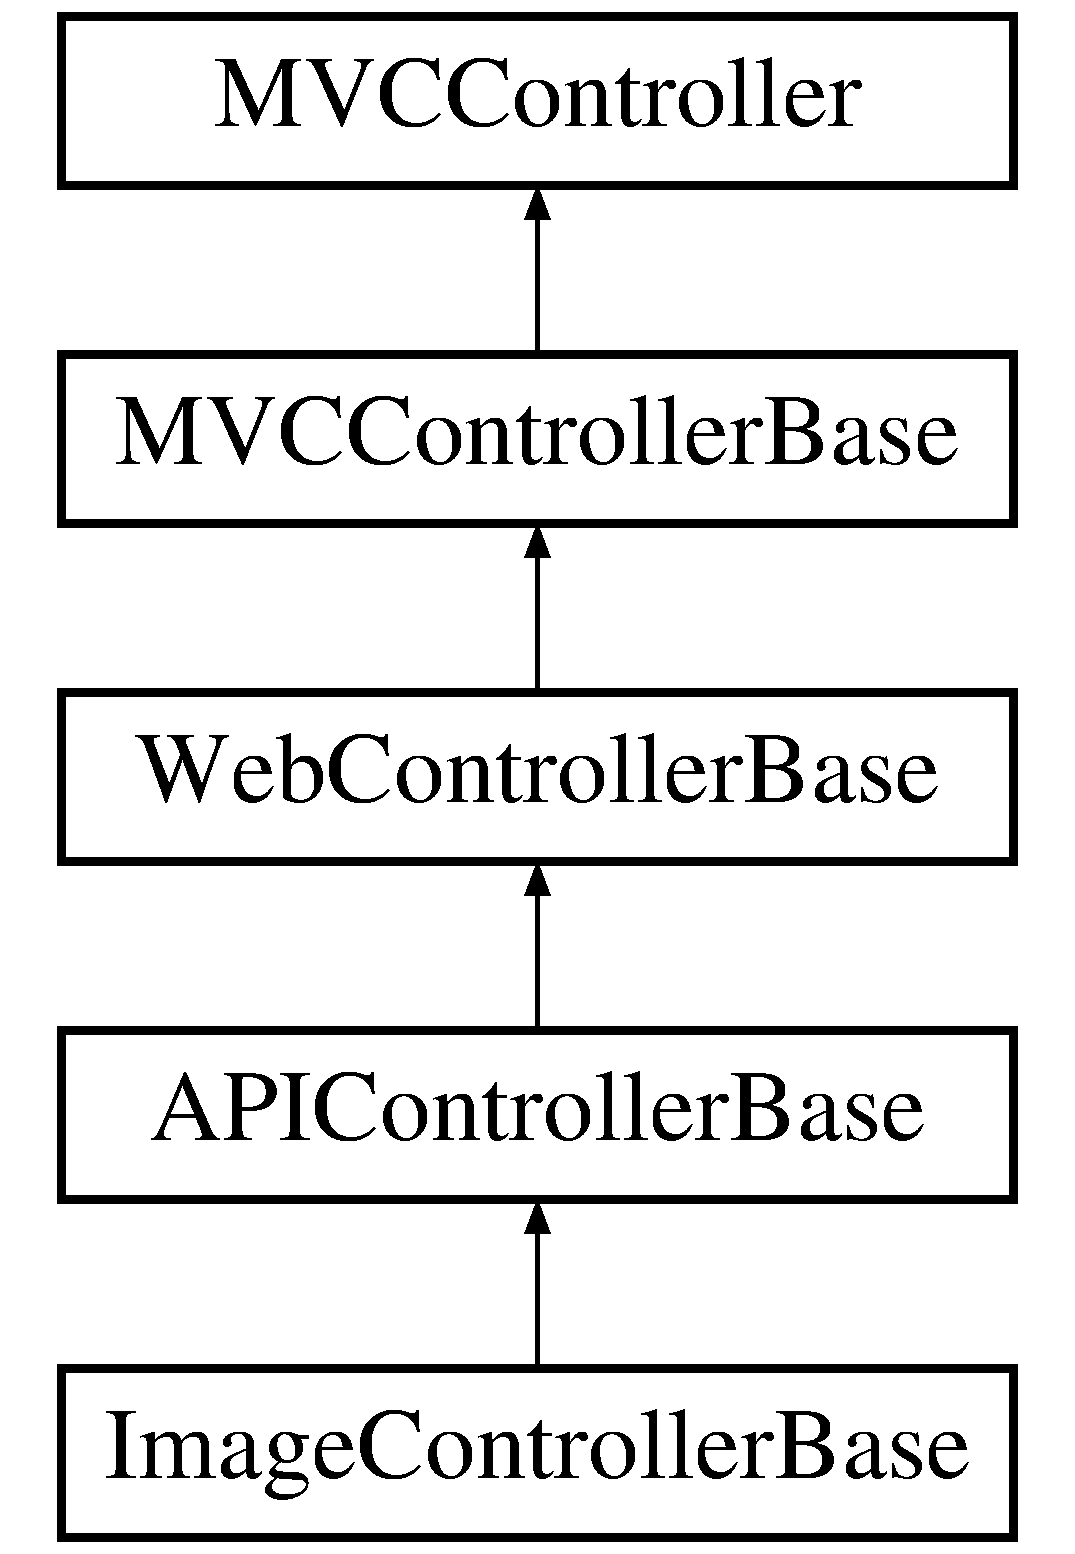
\includegraphics[height=5.000000cm]{class_image_controller_base}
\end{center}
\end{figure}
\subsection*{公開変数類}
\begin{DoxyCompactItemize}
\item 
\hypertarget{class_image_controller_base_a48518f64bd926bab64265066a1aa6145}{}{\bfseries \$http\+Status} = 200\label{class_image_controller_base_a48518f64bd926bab64265066a1aa6145}

\item 
\hypertarget{class_image_controller_base_a46898a279a531bb5e6c8b0fe0e15d1cd}{}{\bfseries \$output\+Type} = \char`\"{}\char`\"{}\label{class_image_controller_base_a46898a279a531bb5e6c8b0fe0e15d1cd}

\end{DoxyCompactItemize}
\subsection*{限定公開メンバ関数}
\begin{DoxyCompactItemize}
\item 
\hyperlink{class_image_controller_base_a0eaea96edabf75b7ac4da68173ab4c56}{\+\_\+get\+Image} (\$arg\+File\+Path, \$arg\+Width=N\+U\+L\+L, \$arg\+Height=N\+U\+L\+L, \$arg\+Proportional=N\+U\+L\+L, \$arg\+Memcache\+D\+S\+N=N\+U\+L\+L)
\end{DoxyCompactItemize}
\subsection*{その他の継承メンバ}


\subsection{関数詳解}
\hypertarget{class_image_controller_base_a0eaea96edabf75b7ac4da68173ab4c56}{}\index{Image\+Controller\+Base@{Image\+Controller\+Base}!\+\_\+get\+Image@{\+\_\+get\+Image}}
\index{\+\_\+get\+Image@{\+\_\+get\+Image}!Image\+Controller\+Base@{Image\+Controller\+Base}}
\subsubsection[{\+\_\+get\+Image}]{\setlength{\rightskip}{0pt plus 5cm}Image\+Controller\+Base\+::\+\_\+get\+Image (
\begin{DoxyParamCaption}
\item[{}]{\$arg\+File\+Path, }
\item[{}]{\$arg\+Width = {\ttfamily NULL}, }
\item[{}]{\$arg\+Height = {\ttfamily NULL}, }
\item[{}]{\$arg\+Proportional = {\ttfamily NULL}, }
\item[{}]{\$arg\+Memcache\+D\+S\+N = {\ttfamily NULL}}
\end{DoxyParamCaption}
)\hspace{0.3cm}{\ttfamily [protected]}}\label{class_image_controller_base_a0eaea96edabf75b7ac4da68173ab4c56}

\begin{DoxyParams}[1]{引数}
unknown & {\em \$arg\+File\+Path} & \\
\hline
string & {\em \$arg\+Width} & \\
\hline
string & {\em \$arg\+Height} & \\
\hline
string & {\em \$arg\+Proportional} & true\+:サイズ上の縦横比を維持しつつ、縮小する false\+:指定された比率にリサイズ(アスペクト比は変わらない) \\
\hline
string & {\em \$arg\+Memcache\+D\+S\+N} & \\
\hline
\end{DoxyParams}
\begin{DoxyReturn}{戻り値}
boolean 
\end{DoxyReturn}


このクラス詳解は次のファイルから抽出されました\+:\begin{DoxyCompactItemize}
\item 
Framework\+Package/class/\+M\+V\+C/Image\+Controller\+Base.\+class.\+php\end{DoxyCompactItemize}

\hypertarget{class_image_info}{}\section{Image\+Info クラス}
\label{class_image_info}\index{Image\+Info@{Image\+Info}}
\subsection*{静的公開メンバ関数}
\begin{DoxyCompactItemize}
\item 
static \& \hyperlink{class_image_info_a4bab7c33da9789d92c14dab790562fa1}{get\+Info\+From\+File} (\$filename)
\item 
static \& \hyperlink{class_image_info_a7ce19e9a5da702ba3c0b3c7163d55663}{get\+Info\+From\+Data} (\&\$data)
\end{DoxyCompactItemize}


\subsection{詳解}
ファイル、またはバイナリデータから画像の情報を取得するクラス インスタンス化せず、以下のように静的に呼び出して使用します。

\$result = \hyperlink{class_image_info_a4bab7c33da9789d92c14dab790562fa1}{Image\+Info\+::get\+Info\+From\+File}(\textquotesingle{}/xxx/xxx.xxx\textquotesingle{}); 

\subsection{関数詳解}
\hypertarget{class_image_info_a7ce19e9a5da702ba3c0b3c7163d55663}{}\index{Image\+Info@{Image\+Info}!get\+Info\+From\+Data@{get\+Info\+From\+Data}}
\index{get\+Info\+From\+Data@{get\+Info\+From\+Data}!Image\+Info@{Image\+Info}}
\subsubsection[{get\+Info\+From\+Data}]{\setlength{\rightskip}{0pt plus 5cm}static\& Image\+Info\+::get\+Info\+From\+Data (
\begin{DoxyParamCaption}
\item[{\&}]{\$data}
\end{DoxyParamCaption}
)\hspace{0.3cm}{\ttfamily [static]}}\label{class_image_info_a7ce19e9a5da702ba3c0b3c7163d55663}
バイナリデータから\+Image\+Info\+Resultオブジェクトを生成して返す


\begin{DoxyParams}[1]{引数}
string & {\em \&\$data} & バイナリデータ \\
\hline
\end{DoxyParams}
\begin{DoxyReturn}{戻り値}
object Image\+Info\+Resultオブジェクト 
\end{DoxyReturn}
\hypertarget{class_image_info_a4bab7c33da9789d92c14dab790562fa1}{}\index{Image\+Info@{Image\+Info}!get\+Info\+From\+File@{get\+Info\+From\+File}}
\index{get\+Info\+From\+File@{get\+Info\+From\+File}!Image\+Info@{Image\+Info}}
\subsubsection[{get\+Info\+From\+File}]{\setlength{\rightskip}{0pt plus 5cm}static\& Image\+Info\+::get\+Info\+From\+File (
\begin{DoxyParamCaption}
\item[{}]{\$filename}
\end{DoxyParamCaption}
)\hspace{0.3cm}{\ttfamily [static]}}\label{class_image_info_a4bab7c33da9789d92c14dab790562fa1}
ファイルから\+Image\+Info\+Resultオブジェクトを生成して返す


\begin{DoxyParams}[1]{引数}
string & {\em \$filename} & ファイル名 \\
\hline
\end{DoxyParams}
\begin{DoxyReturn}{戻り値}
object Image\+Info\+Resultオブジェクト 
\end{DoxyReturn}


このクラス詳解は次のファイルから抽出されました\+:\begin{DoxyCompactItemize}
\item 
Generic\+Package/class/\+Image/Image.\+class.\+php\end{DoxyCompactItemize}

\hypertarget{class_image_info___gif}{}\section{Image\+Info\+\_\+\+Gif クラス}
\label{class_image_info___gif}\index{Image\+Info\+\_\+\+Gif@{Image\+Info\+\_\+\+Gif}}
\subsection*{公開メンバ関数}
\begin{DoxyCompactItemize}
\item 
\hyperlink{class_image_info___gif_a901790c8747944166a84d47db8436751}{get\+Info} (\&\$data, \&\$image\+\_\+info)
\end{DoxyCompactItemize}
\subsection*{静的公開メンバ関数}
\begin{DoxyCompactItemize}
\item 
static \hyperlink{class_image_info___gif_a9516f27349ef6cb8303fde07c587e8d8}{is\+Valid} (\&\$data)
\end{DoxyCompactItemize}


\subsection{詳解}
G\+I\+F画像の情報を処理するクラス  private 

\subsection{関数詳解}
\hypertarget{class_image_info___gif_a901790c8747944166a84d47db8436751}{}\index{Image\+Info\+\_\+\+Gif@{Image\+Info\+\_\+\+Gif}!get\+Info@{get\+Info}}
\index{get\+Info@{get\+Info}!Image\+Info\+\_\+\+Gif@{Image\+Info\+\_\+\+Gif}}
\subsubsection[{get\+Info}]{\setlength{\rightskip}{0pt plus 5cm}Image\+Info\+\_\+\+Gif\+::get\+Info (
\begin{DoxyParamCaption}
\item[{\&}]{\$data, }
\item[{\&}]{\$image\+\_\+info}
\end{DoxyParamCaption}
)}\label{class_image_info___gif_a901790c8747944166a84d47db8436751}
バイナリデータから\+G\+I\+F画像の情報を取得して返す


\begin{DoxyParams}[1]{引数}
string & {\em \&\$data} & 画像のバイナリデータ \\
\hline
array & {\em \&\$image\+\_\+info} & 取得した画像情報を格納する配列\\
\hline
\end{DoxyParams}
\begin{DoxyReturn}{戻り値}
boolean true =$>$ 情報の取得に成功 false =$>$ エラー発生 
\end{DoxyReturn}
\hypertarget{class_image_info___gif_a9516f27349ef6cb8303fde07c587e8d8}{}\index{Image\+Info\+\_\+\+Gif@{Image\+Info\+\_\+\+Gif}!is\+Valid@{is\+Valid}}
\index{is\+Valid@{is\+Valid}!Image\+Info\+\_\+\+Gif@{Image\+Info\+\_\+\+Gif}}
\subsubsection[{is\+Valid}]{\setlength{\rightskip}{0pt plus 5cm}static Image\+Info\+\_\+\+Gif\+::is\+Valid (
\begin{DoxyParamCaption}
\item[{\&}]{\$data}
\end{DoxyParamCaption}
)\hspace{0.3cm}{\ttfamily [static]}}\label{class_image_info___gif_a9516f27349ef6cb8303fde07c587e8d8}
有効な\+J\+P\+E\+Gファイルのデータであるかを判定する


\begin{DoxyParams}[1]{引数}
string & {\em \&\$data} & 画像のバイナリデータ \\
\hline
\end{DoxyParams}
\begin{DoxyReturn}{戻り値}
boolean true =$>$ P\+N\+G画像 false =$>$ P\+N\+G画像ではない 
\end{DoxyReturn}


このクラス詳解は次のファイルから抽出されました\+:\begin{DoxyCompactItemize}
\item 
Generic\+Package/class/\+Image/Image.\+class.\+php\end{DoxyCompactItemize}

\hypertarget{class_image_info___jpeg}{}\section{Image\+Info\+\_\+\+Jpeg クラス}
\label{class_image_info___jpeg}\index{Image\+Info\+\_\+\+Jpeg@{Image\+Info\+\_\+\+Jpeg}}
\subsection*{公開メンバ関数}
\begin{DoxyCompactItemize}
\item 
\hyperlink{class_image_info___jpeg_aad43653da2d84f9d503561f110fa819e}{get\+Info} (\&\$data, \&\$image\+\_\+info)
\end{DoxyCompactItemize}
\subsection*{静的公開メンバ関数}
\begin{DoxyCompactItemize}
\item 
static \hyperlink{class_image_info___jpeg_ae6336be504ffe67dd34964fa4557d338}{is\+Valid} (\&\$data)
\end{DoxyCompactItemize}
\subsection*{公開変数類}
\begin{DoxyCompactItemize}
\item 
\hypertarget{class_image_info___jpeg_ad65b973cd1b699c17e15f2b9689039c2}{}{\bfseries \$jpeg\+\_\+type}\label{class_image_info___jpeg_ad65b973cd1b699c17e15f2b9689039c2}

\end{DoxyCompactItemize}


\subsection{詳解}
J\+P\+E\+G画像の情報を処理するクラス

ベースライン方式、プログレッシブ形式のみに対応しています。  private 

\subsection{関数詳解}
\hypertarget{class_image_info___jpeg_aad43653da2d84f9d503561f110fa819e}{}\index{Image\+Info\+\_\+\+Jpeg@{Image\+Info\+\_\+\+Jpeg}!get\+Info@{get\+Info}}
\index{get\+Info@{get\+Info}!Image\+Info\+\_\+\+Jpeg@{Image\+Info\+\_\+\+Jpeg}}
\subsubsection[{get\+Info}]{\setlength{\rightskip}{0pt plus 5cm}Image\+Info\+\_\+\+Jpeg\+::get\+Info (
\begin{DoxyParamCaption}
\item[{\&}]{\$data, }
\item[{\&}]{\$image\+\_\+info}
\end{DoxyParamCaption}
)}\label{class_image_info___jpeg_aad43653da2d84f9d503561f110fa819e}
バイナリデータから\+J\+P\+E\+G画像の情報を取得して返す


\begin{DoxyParams}[1]{引数}
string & {\em \&\$data} & 画像のバイナリデータ \\
\hline
array & {\em \&\$image\+\_\+info} & 取得した画像情報を格納する配列\\
\hline
\end{DoxyParams}
\begin{DoxyReturn}{戻り値}
boolean true =$>$ 情報の取得に成功 false =$>$ エラー発生 
\end{DoxyReturn}
\hypertarget{class_image_info___jpeg_ae6336be504ffe67dd34964fa4557d338}{}\index{Image\+Info\+\_\+\+Jpeg@{Image\+Info\+\_\+\+Jpeg}!is\+Valid@{is\+Valid}}
\index{is\+Valid@{is\+Valid}!Image\+Info\+\_\+\+Jpeg@{Image\+Info\+\_\+\+Jpeg}}
\subsubsection[{is\+Valid}]{\setlength{\rightskip}{0pt plus 5cm}static Image\+Info\+\_\+\+Jpeg\+::is\+Valid (
\begin{DoxyParamCaption}
\item[{\&}]{\$data}
\end{DoxyParamCaption}
)\hspace{0.3cm}{\ttfamily [static]}}\label{class_image_info___jpeg_ae6336be504ffe67dd34964fa4557d338}
有効な\+J\+P\+E\+Gファイルのデータであるかを判定する


\begin{DoxyParams}[1]{引数}
string & {\em \&\$data} & 画像のバイナリデータ \\
\hline
\end{DoxyParams}
\begin{DoxyReturn}{戻り値}
boolean true =$>$ J\+P\+E\+G画像 false =$>$ J\+P\+E\+G画像ではない 
\end{DoxyReturn}


このクラス詳解は次のファイルから抽出されました\+:\begin{DoxyCompactItemize}
\item 
Generic\+Package/class/\+Image/Image.\+class.\+php\end{DoxyCompactItemize}

\hypertarget{class_image_info___png}{}\section{Image\+Info\+\_\+\+Png クラス}
\label{class_image_info___png}\index{Image\+Info\+\_\+\+Png@{Image\+Info\+\_\+\+Png}}
\subsection*{公開メンバ関数}
\begin{DoxyCompactItemize}
\item 
\hyperlink{class_image_info___png_aef4e82df37b227b91e7ac334b19c6e36}{get\+Info} (\&\$data, \&\$image\+\_\+info)
\end{DoxyCompactItemize}
\subsection*{静的公開メンバ関数}
\begin{DoxyCompactItemize}
\item 
static \hyperlink{class_image_info___png_afa5c6fb4ffa45b64e3106e498ab962d8}{is\+Valid} (\&\$data)
\end{DoxyCompactItemize}


\subsection{詳解}
P\+N\+G画像の情報を処理するクラス  private 

\subsection{関数詳解}
\hypertarget{class_image_info___png_aef4e82df37b227b91e7ac334b19c6e36}{}\index{Image\+Info\+\_\+\+Png@{Image\+Info\+\_\+\+Png}!get\+Info@{get\+Info}}
\index{get\+Info@{get\+Info}!Image\+Info\+\_\+\+Png@{Image\+Info\+\_\+\+Png}}
\subsubsection[{get\+Info}]{\setlength{\rightskip}{0pt plus 5cm}Image\+Info\+\_\+\+Png\+::get\+Info (
\begin{DoxyParamCaption}
\item[{\&}]{\$data, }
\item[{\&}]{\$image\+\_\+info}
\end{DoxyParamCaption}
)}\label{class_image_info___png_aef4e82df37b227b91e7ac334b19c6e36}
バイナリデータから\+P\+N\+G画像の情報を取得して返す


\begin{DoxyParams}[1]{引数}
string & {\em \&\$data} & 画像のバイナリデータ \\
\hline
array & {\em \&\$image\+\_\+info} & 取得した画像情報を格納する配列\\
\hline
\end{DoxyParams}
\begin{DoxyReturn}{戻り値}
boolean true =$>$ 情報の取得に成功 false =$>$ エラー発生 
\end{DoxyReturn}
\hypertarget{class_image_info___png_afa5c6fb4ffa45b64e3106e498ab962d8}{}\index{Image\+Info\+\_\+\+Png@{Image\+Info\+\_\+\+Png}!is\+Valid@{is\+Valid}}
\index{is\+Valid@{is\+Valid}!Image\+Info\+\_\+\+Png@{Image\+Info\+\_\+\+Png}}
\subsubsection[{is\+Valid}]{\setlength{\rightskip}{0pt plus 5cm}static Image\+Info\+\_\+\+Png\+::is\+Valid (
\begin{DoxyParamCaption}
\item[{\&}]{\$data}
\end{DoxyParamCaption}
)\hspace{0.3cm}{\ttfamily [static]}}\label{class_image_info___png_afa5c6fb4ffa45b64e3106e498ab962d8}
有効な\+J\+P\+E\+Gファイルのデータであるかを判定する


\begin{DoxyParams}[1]{引数}
string & {\em \&\$data} & 画像のバイナリデータ \\
\hline
\end{DoxyParams}
\begin{DoxyReturn}{戻り値}
boolean true =$>$ P\+N\+G画像 false =$>$ P\+N\+G画像ではない 
\end{DoxyReturn}


このクラス詳解は次のファイルから抽出されました\+:\begin{DoxyCompactItemize}
\item 
Generic\+Package/class/\+Image/Image.\+class.\+php\end{DoxyCompactItemize}

\hypertarget{class_image_info_result}{}\section{Image\+Info\+Result クラス}
\label{class_image_info_result}\index{Image\+Info\+Result@{Image\+Info\+Result}}
\subsection*{公開メンバ関数}
\begin{DoxyCompactItemize}
\item 
\hyperlink{class_image_info_result_a6f13ef7887e6e9d30a17d48dd49a0459}{Image\+Info\+Result} (\$image\+\_\+info)
\item 
\hyperlink{class_image_info_result_a0f0bdd9622bed1b100fbbc342babf48b}{get\+W} ()
\item 
\hyperlink{class_image_info_result_a432f8a200e08c665417025b3f03c64a5}{get\+H} ()
\item 
\hyperlink{class_image_info_result_a0be241535485256c6f67fbd011909a8d}{get\+Type} ()
\item 
\hyperlink{class_image_info_result_acc470f70a838a91c9072c151f21190be}{get\+Colors} ()
\item 
\hyperlink{class_image_info_result_a2a30efa411e4c3c31a2e8132ba58ebce}{is\+Error} ()
\item 
\hyperlink{class_image_info_result_a0e359341fdff21e3821e9e5238bf6946}{get\+Error\+Code} ()
\end{DoxyCompactItemize}
\subsection*{公開変数類}
\begin{DoxyCompactItemize}
\item 
\hypertarget{class_image_info_result_a2ea8cb3d607b605672d33b3d7b600a4f}{}{\bfseries \$w}\label{class_image_info_result_a2ea8cb3d607b605672d33b3d7b600a4f}

\item 
\hypertarget{class_image_info_result_a9f434a13a1510793884fae7395adba0e}{}{\bfseries \$h}\label{class_image_info_result_a9f434a13a1510793884fae7395adba0e}

\item 
\hypertarget{class_image_info_result_a560e7851941e684528edd96fc5e48642}{}{\bfseries \$type}\label{class_image_info_result_a560e7851941e684528edd96fc5e48642}

\item 
\hypertarget{class_image_info_result_af23b27a45577e721edc690b2cbfba5ba}{}{\bfseries \$extension}\label{class_image_info_result_af23b27a45577e721edc690b2cbfba5ba}

\item 
\hypertarget{class_image_info_result_ae4bf606273ed7cbd6e2b765e98bac45e}{}{\bfseries \$colors}\label{class_image_info_result_ae4bf606273ed7cbd6e2b765e98bac45e}

\item 
\hypertarget{class_image_info_result_ae4b25982efeefff62f014d52a562315f}{}{\bfseries \$error\+\_\+flag}\label{class_image_info_result_ae4b25982efeefff62f014d52a562315f}

\item 
\hypertarget{class_image_info_result_a069bb950e4f88c1083434e81b652f790}{}{\bfseries \$error\+\_\+code}\label{class_image_info_result_a069bb950e4f88c1083434e81b652f790}

\end{DoxyCompactItemize}


\subsection{詳解}
画像データの情報を取得した結果を格納するクラス 

\subsection{関数詳解}
\hypertarget{class_image_info_result_acc470f70a838a91c9072c151f21190be}{}\index{Image\+Info\+Result@{Image\+Info\+Result}!get\+Colors@{get\+Colors}}
\index{get\+Colors@{get\+Colors}!Image\+Info\+Result@{Image\+Info\+Result}}
\subsubsection[{get\+Colors}]{\setlength{\rightskip}{0pt plus 5cm}Image\+Info\+Result\+::get\+Colors (
\begin{DoxyParamCaption}
{}
\end{DoxyParamCaption}
)}\label{class_image_info_result_acc470f70a838a91c9072c151f21190be}
色数を返す \begin{DoxyReturn}{戻り値}
int 色数 
\end{DoxyReturn}
\hypertarget{class_image_info_result_a0e359341fdff21e3821e9e5238bf6946}{}\index{Image\+Info\+Result@{Image\+Info\+Result}!get\+Error\+Code@{get\+Error\+Code}}
\index{get\+Error\+Code@{get\+Error\+Code}!Image\+Info\+Result@{Image\+Info\+Result}}
\subsubsection[{get\+Error\+Code}]{\setlength{\rightskip}{0pt plus 5cm}Image\+Info\+Result\+::get\+Error\+Code (
\begin{DoxyParamCaption}
{}
\end{DoxyParamCaption}
)}\label{class_image_info_result_a0e359341fdff21e3821e9e5238bf6946}
エラーコードを返す \begin{DoxyReturn}{戻り値}
int エラーコード。\+Image\+Info\+\_\+\+E\+R\+R\+O\+R\+\_\+\+X\+X\+X 
\end{DoxyReturn}
\hypertarget{class_image_info_result_a432f8a200e08c665417025b3f03c64a5}{}\index{Image\+Info\+Result@{Image\+Info\+Result}!get\+H@{get\+H}}
\index{get\+H@{get\+H}!Image\+Info\+Result@{Image\+Info\+Result}}
\subsubsection[{get\+H}]{\setlength{\rightskip}{0pt plus 5cm}Image\+Info\+Result\+::get\+H (
\begin{DoxyParamCaption}
{}
\end{DoxyParamCaption}
)}\label{class_image_info_result_a432f8a200e08c665417025b3f03c64a5}
縦幅を返す \begin{DoxyReturn}{戻り値}
int 縦幅 
\end{DoxyReturn}
\hypertarget{class_image_info_result_a0be241535485256c6f67fbd011909a8d}{}\index{Image\+Info\+Result@{Image\+Info\+Result}!get\+Type@{get\+Type}}
\index{get\+Type@{get\+Type}!Image\+Info\+Result@{Image\+Info\+Result}}
\subsubsection[{get\+Type}]{\setlength{\rightskip}{0pt plus 5cm}Image\+Info\+Result\+::get\+Type (
\begin{DoxyParamCaption}
{}
\end{DoxyParamCaption}
)}\label{class_image_info_result_a0be241535485256c6f67fbd011909a8d}
画像の種類を返す \begin{DoxyReturn}{戻り値}
int 画像の種類。(\+I\+M\+A\+G\+E\+T\+Y\+P\+E\+\_\+\+X\+X\+X) 
\end{DoxyReturn}
\hypertarget{class_image_info_result_a0f0bdd9622bed1b100fbbc342babf48b}{}\index{Image\+Info\+Result@{Image\+Info\+Result}!get\+W@{get\+W}}
\index{get\+W@{get\+W}!Image\+Info\+Result@{Image\+Info\+Result}}
\subsubsection[{get\+W}]{\setlength{\rightskip}{0pt plus 5cm}Image\+Info\+Result\+::get\+W (
\begin{DoxyParamCaption}
{}
\end{DoxyParamCaption}
)}\label{class_image_info_result_a0f0bdd9622bed1b100fbbc342babf48b}
横幅を返す \begin{DoxyReturn}{戻り値}
int 横幅 
\end{DoxyReturn}
\hypertarget{class_image_info_result_a6f13ef7887e6e9d30a17d48dd49a0459}{}\index{Image\+Info\+Result@{Image\+Info\+Result}!Image\+Info\+Result@{Image\+Info\+Result}}
\index{Image\+Info\+Result@{Image\+Info\+Result}!Image\+Info\+Result@{Image\+Info\+Result}}
\subsubsection[{Image\+Info\+Result}]{\setlength{\rightskip}{0pt plus 5cm}Image\+Info\+Result\+::\+Image\+Info\+Result (
\begin{DoxyParamCaption}
\item[{}]{\$image\+\_\+info}
\end{DoxyParamCaption}
)}\label{class_image_info_result_a6f13ef7887e6e9d30a17d48dd49a0459}
コンストラクタ。画像の情報をセットする。


\begin{DoxyParams}[1]{引数}
array & {\em \$image\+\_\+info} & 画像の情報を含む配列
\begin{DoxyItemize}
\item \$arr\mbox{[}\textquotesingle{}w\textquotesingle{}\mbox{]} = 横幅
\item \$arr\mbox{[}\textquotesingle{}h\textquotesingle{}\mbox{]} = 横幅
\item \$arr\mbox{[}\textquotesingle{}type\textquotesingle{}\mbox{]} = 画像の種類(\+I\+M\+A\+G\+E\+T\+Y\+P\+E\+\_\+\+X\+X\+X)
\item \$arr\mbox{[}\textquotesingle{}extension\textquotesingle{}\mbox{]} = 画像の拡張子(jpg$\vert$gif$\vert$png)
\item \$arr\mbox{[}\textquotesingle{}colors\textquotesingle{}\mbox{]} = 色数
\item \$arr\mbox{[}\textquotesingle{}error\textquotesingle{}\mbox{]} = エラーコード 
\end{DoxyItemize}\\
\hline
\end{DoxyParams}
\hypertarget{class_image_info_result_a2a30efa411e4c3c31a2e8132ba58ebce}{}\index{Image\+Info\+Result@{Image\+Info\+Result}!is\+Error@{is\+Error}}
\index{is\+Error@{is\+Error}!Image\+Info\+Result@{Image\+Info\+Result}}
\subsubsection[{is\+Error}]{\setlength{\rightskip}{0pt plus 5cm}Image\+Info\+Result\+::is\+Error (
\begin{DoxyParamCaption}
{}
\end{DoxyParamCaption}
)}\label{class_image_info_result_a2a30efa411e4c3c31a2e8132ba58ebce}
エラーがあったかどうかを返す \begin{DoxyReturn}{戻り値}
boolean true =$>$ エラーあり false =$>$ エラーなし 
\end{DoxyReturn}


このクラス詳解は次のファイルから抽出されました\+:\begin{DoxyCompactItemize}
\item 
Generic\+Package/class/\+Image/Image.\+class.\+php\end{DoxyCompactItemize}

\hypertarget{class_image_util}{}\section{Image\+Util クラス}
\label{class_image_util}\index{Image\+Util@{Image\+Util}}
\subsection*{静的公開メンバ関数}
\begin{DoxyCompactItemize}
\item 
\hypertarget{class_image_util_ad1ddd6ecbd5291ec88d3eba7cea0ac30}{}static {\bfseries crop} (\$arg\+Image\+Binary, \$arg\+Crop\+Left=0, \$arg\+Crop\+Top=0, \$arg\+Crop\+Right=0, \$arg\+Crop\+Bottom=0)\label{class_image_util_ad1ddd6ecbd5291ec88d3eba7cea0ac30}

\item 
\hypertarget{class_image_util_ae3dbf76ea97f32b35fe4842eb4352d96}{}static {\bfseries resize} (\$arg\+Image\+Binary, \$width=0, \$height=0, \$proportional=false)\label{class_image_util_ae3dbf76ea97f32b35fe4842eb4352d96}

\end{DoxyCompactItemize}


\subsection{詳解}
Imgae\+Infoと依存して、画像を色々する画像\+Util 

このクラス詳解は次のファイルから抽出されました\+:\begin{DoxyCompactItemize}
\item 
Generic\+Package/class/\+Image/Image.\+class.\+php\end{DoxyCompactItemize}

\hypertarget{class_lib_x_m_l_exception}{}\section{Lib\+X\+M\+L\+Exception クラス}
\label{class_lib_x_m_l_exception}\index{Lib\+X\+M\+L\+Exception@{Lib\+X\+M\+L\+Exception}}
Lib\+X\+M\+L\+Exception の継承関係図\begin{figure}[H]
\begin{center}
\leavevmode
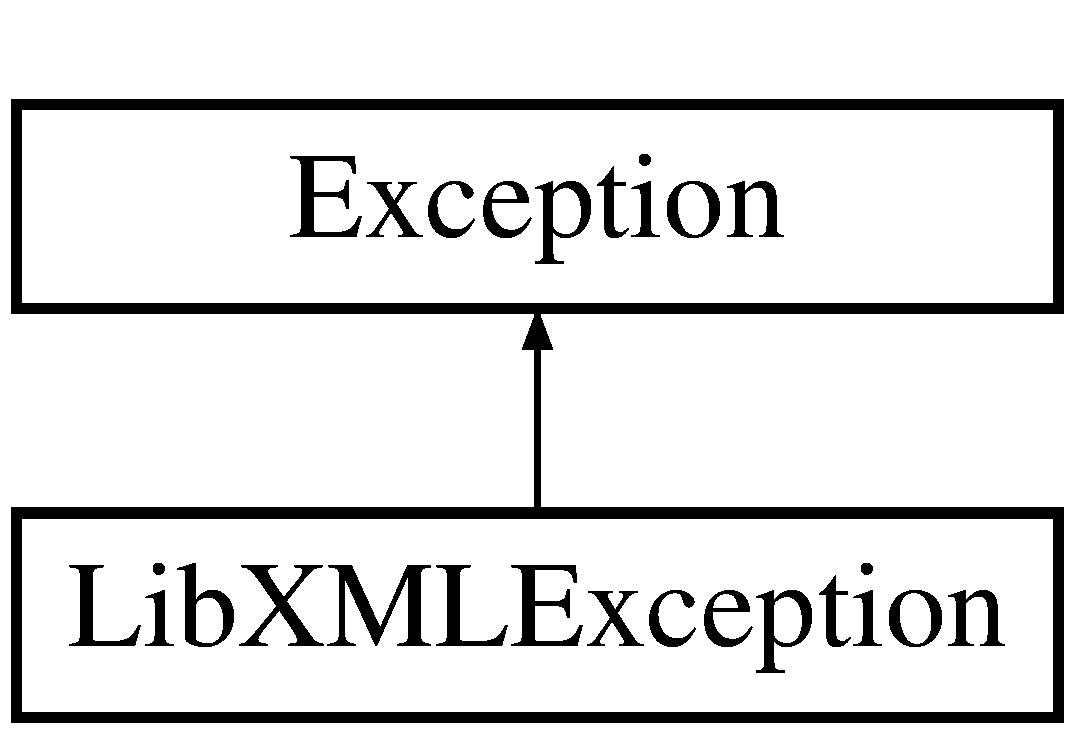
\includegraphics[height=2.000000cm]{class_lib_x_m_l_exception}
\end{center}
\end{figure}
\subsection*{公開メンバ関数}
\begin{DoxyCompactItemize}
\item 
\hypertarget{class_lib_x_m_l_exception_ab39c6f0b2de0f7c0320f7f0e4d127895}{}{\bfseries \+\_\+\+\_\+construct} (\$arg\+Lib\+X\+M\+L\+Errors, \$arg\+Code=N\+U\+L\+L, \$arg\+Previus=N\+U\+L\+L)\label{class_lib_x_m_l_exception_ab39c6f0b2de0f7c0320f7f0e4d127895}

\end{DoxyCompactItemize}


このクラス詳解は次のファイルから抽出されました\+:\begin{DoxyCompactItemize}
\item 
Generic\+Package/class/\+Exception/Lib\+X\+M\+L\+Exception.\+class.\+php\end{DoxyCompactItemize}

\hypertarget{interface_m_v_c_controller}{}\section{M\+V\+C\+Controller インタフェース}
\label{interface_m_v_c_controller}\index{M\+V\+C\+Controller@{M\+V\+C\+Controller}}
M\+V\+C\+Controller の継承関係図\begin{figure}[H]
\begin{center}
\leavevmode
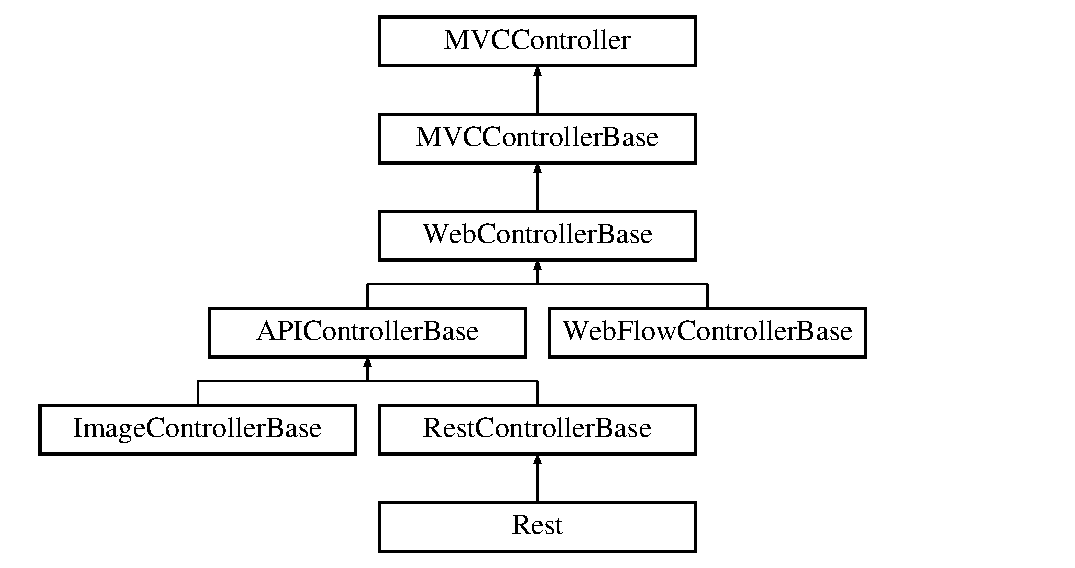
\includegraphics[height=6.000000cm]{interface_m_v_c_controller}
\end{center}
\end{figure}
\subsection*{公開メンバ関数}
\begin{DoxyCompactItemize}
\item 
\hyperlink{interface_m_v_c_controller_aa32412dfd3a8ea546559a57007a3fe7b}{execute} ()
\end{DoxyCompactItemize}


\subsection{関数詳解}
\hypertarget{interface_m_v_c_controller_aa32412dfd3a8ea546559a57007a3fe7b}{}\index{M\+V\+C\+Controller@{M\+V\+C\+Controller}!execute@{execute}}
\index{execute@{execute}!M\+V\+C\+Controller@{M\+V\+C\+Controller}}
\subsubsection[{execute}]{\setlength{\rightskip}{0pt plus 5cm}M\+V\+C\+Controller\+::execute (
\begin{DoxyParamCaption}
{}
\end{DoxyParamCaption}
)}\label{interface_m_v_c_controller_aa32412dfd3a8ea546559a57007a3fe7b}
デフォルトアクションメソッド 

\hyperlink{class_m_v_c_controller_base_a333dc4807e54360e6ca3966563f8bc56}{M\+V\+C\+Controller\+Base}で実装されています。



このインタフェース詳解は次のファイルから抽出されました\+:\begin{DoxyCompactItemize}
\item 
Framework\+Package/class/\+M\+V\+C/M\+V\+C\+Controller.\+interface.\+php\end{DoxyCompactItemize}

\hypertarget{class_m_v_c_controller_base}{}\section{M\+V\+C\+Controller\+Base クラス}
\label{class_m_v_c_controller_base}\index{M\+V\+C\+Controller\+Base@{M\+V\+C\+Controller\+Base}}
M\+V\+C\+Controller\+Base の継承関係図\begin{figure}[H]
\begin{center}
\leavevmode
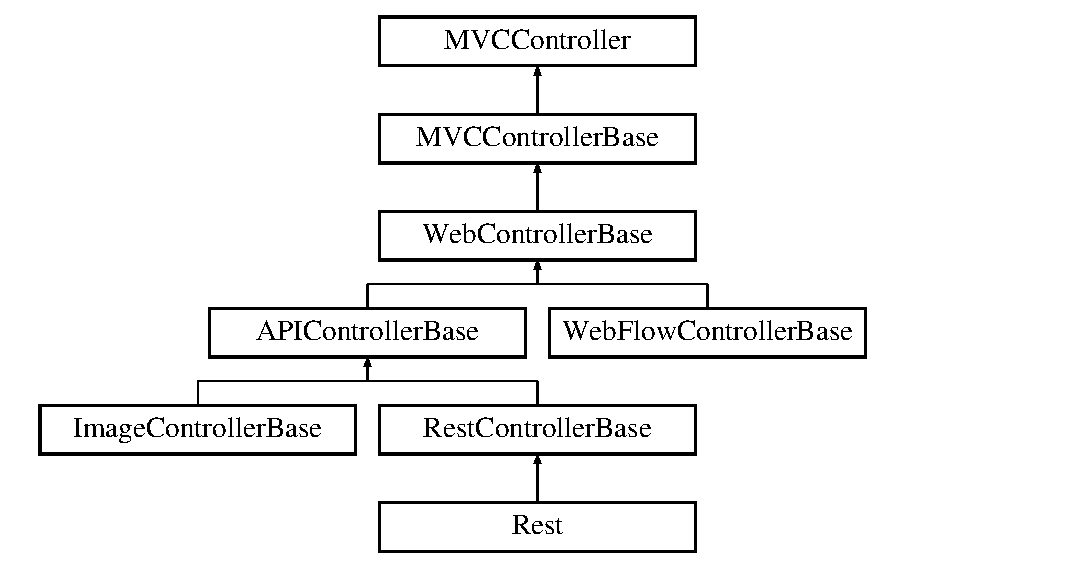
\includegraphics[height=6.000000cm]{class_m_v_c_controller_base}
\end{center}
\end{figure}
\subsection*{公開メンバ関数}
\begin{DoxyCompactItemize}
\item 
\hyperlink{class_m_v_c_controller_base_a333dc4807e54360e6ca3966563f8bc56}{execute} ()
\end{DoxyCompactItemize}
\subsection*{公開変数類}
\begin{DoxyCompactItemize}
\item 
\hypertarget{class_m_v_c_controller_base_ac93554590de5a9fa1d9d14132a0bfd7a}{}{\bfseries \$controler\+Class\+Name} = \char`\"{}\char`\"{}\label{class_m_v_c_controller_base_ac93554590de5a9fa1d9d14132a0bfd7a}

\item 
\hypertarget{class_m_v_c_controller_base_acf02ad9e097c55c3336b15a400c3cb8b}{}{\bfseries \$http\+Status} = 200\label{class_m_v_c_controller_base_acf02ad9e097c55c3336b15a400c3cb8b}

\item 
\hypertarget{class_m_v_c_controller_base_a6c73e4b25e1a4e0a40c65224c0f1964b}{}{\bfseries \$output\+Type} = \char`\"{}html\char`\"{}\label{class_m_v_c_controller_base_a6c73e4b25e1a4e0a40c65224c0f1964b}

\item 
\hypertarget{class_m_v_c_controller_base_a841fa7809ce635f4b0b9839a63eef8af}{}{\bfseries \$request\+Method} = \char`\"{}G\+E\+T\char`\"{}\label{class_m_v_c_controller_base_a841fa7809ce635f4b0b9839a63eef8af}

\item 
\hypertarget{class_m_v_c_controller_base_a2061872d0215e9a5a08e66938a2097b7}{}{\bfseries \$rest\+Resource} = \textquotesingle{}\textquotesingle{}\label{class_m_v_c_controller_base_a2061872d0215e9a5a08e66938a2097b7}

\item 
\hypertarget{class_m_v_c_controller_base_af816a433553d35ae3bf5f9d5ae61e899}{}{\bfseries \$json\+Unescaped\+Unicode} = T\+R\+U\+E\label{class_m_v_c_controller_base_af816a433553d35ae3bf5f9d5ae61e899}

\item 
\hypertarget{class_m_v_c_controller_base_ae70d838e98b8aa9329feb8a7aa6e2e9b}{}{\bfseries \$device\+Type} = \char`\"{}P\+C\char`\"{}\label{class_m_v_c_controller_base_ae70d838e98b8aa9329feb8a7aa6e2e9b}

\item 
\hypertarget{class_m_v_c_controller_base_ab363a54f929a5a7cda8ccb2c3a7196fa}{}{\bfseries \$app\+Version} = \char`\"{}1.\+0.\+0\char`\"{}\label{class_m_v_c_controller_base_ab363a54f929a5a7cda8ccb2c3a7196fa}

\item 
\hypertarget{class_m_v_c_controller_base_ab9ee1ae1966371f115334bc8119dd4b4}{}{\bfseries \$apple\+Reviewd} = F\+A\+L\+S\+E\label{class_m_v_c_controller_base_ab9ee1ae1966371f115334bc8119dd4b4}

\item 
\hypertarget{class_m_v_c_controller_base_a65caef2110c8d21b6ec65a2a03f9bdbe}{}{\bfseries \$must\+App\+Versioned} = F\+A\+L\+S\+E\label{class_m_v_c_controller_base_a65caef2110c8d21b6ec65a2a03f9bdbe}

\item 
\hypertarget{class_m_v_c_controller_base_af637663bfb89da6beba8eead3bc408c7}{}{\bfseries \$allowed} = N\+U\+L\+L\label{class_m_v_c_controller_base_af637663bfb89da6beba8eead3bc408c7}

\end{DoxyCompactItemize}


\subsection{関数詳解}
\hypertarget{class_m_v_c_controller_base_a333dc4807e54360e6ca3966563f8bc56}{}\index{M\+V\+C\+Controller\+Base@{M\+V\+C\+Controller\+Base}!execute@{execute}}
\index{execute@{execute}!M\+V\+C\+Controller\+Base@{M\+V\+C\+Controller\+Base}}
\subsubsection[{execute}]{\setlength{\rightskip}{0pt plus 5cm}M\+V\+C\+Controller\+Base\+::execute (
\begin{DoxyParamCaption}
{}
\end{DoxyParamCaption}
)}\label{class_m_v_c_controller_base_a333dc4807e54360e6ca3966563f8bc56}
デフォルトアクションメソッド 

\hyperlink{interface_m_v_c_controller_aa32412dfd3a8ea546559a57007a3fe7b}{M\+V\+C\+Controller}を実装しています。



このクラス詳解は次のファイルから抽出されました\+:\begin{DoxyCompactItemize}
\item 
Framework\+Package/class/\+M\+V\+C/M\+V\+C\+Controller\+Base.\+abstract.\+php\end{DoxyCompactItemize}

\hypertarget{class_m_v_c_core}{}\section{M\+V\+C\+Core クラス}
\label{class_m_v_c_core}\index{M\+V\+C\+Core@{M\+V\+C\+Core}}
\subsection*{静的公開メンバ関数}
\begin{DoxyCompactItemize}
\item 
static \hyperlink{class_m_v_c_core_a586d3831211555544f39242a2eddd1d9}{webmain} (\$arg\+Flow\+X\+M\+L\+Base\+Path= \textquotesingle{}\textquotesingle{})
\item 
\hypertarget{class_m_v_c_core_aef631bde3989df4f2b34685a4cf6878c}{}static {\bfseries consolemain} (\$arg\+Flow\+X\+M\+L\+Base\+Path= \textquotesingle{}\textquotesingle{})\label{class_m_v_c_core_aef631bde3989df4f2b34685a4cf6878c}

\item 
static \hyperlink{class_m_v_c_core_af300736b8ef9af5c298e16b91cdb68e1}{load\+M\+V\+C\+Module} (\$arg\+Class\+Name=N\+U\+L\+L, \$arg\+Class\+Exists\+Called=F\+A\+L\+S\+E, \$arg\+Target\+Path= \textquotesingle{}\textquotesingle{})
\item 
static \hyperlink{class_m_v_c_core_a728cd61380f5331ee3420ff4a8f3ae10}{load\+M\+V\+C\+Filter} (\$arg\+Filter\+Name, \$arg\+Target\+Path= \textquotesingle{}\textquotesingle{})
\item 
static \hyperlink{class_m_v_c_core_ae4f2a29faa032b6a092593a5bbe5a5b5}{load\+Template} (\$arg\+Class\+Name=N\+U\+L\+L, \$arg\+File\+Exists\+Called=F\+A\+L\+S\+E, \$arg\+Target\+Path= \textquotesingle{}\textquotesingle{}, \$arg\+View\+Type=F\+A\+L\+S\+E, \$arg\+Template\+Engine= \textquotesingle{}\hyperlink{class_html_view_assignor}{Html\+View\+Assignor}\textquotesingle{})
\item 
static \hyperlink{class_m_v_c_core_ae5c6d4b499b71f7ddb02eeba80d185e0}{load\+View} (\$arg\+Class\+Name=N\+U\+L\+L, \$arg\+File\+Exists\+Called=F\+A\+L\+S\+E, \$arg\+Target\+Path= \textquotesingle{}\textquotesingle{}, \$arg\+View\+Type=F\+A\+L\+S\+E)
\end{DoxyCompactItemize}
\subsection*{静的公開変数類}
\begin{DoxyCompactItemize}
\item 
\hypertarget{class_m_v_c_core_a59f8bd5d7e677495ba29e8e1db414682}{}static {\bfseries \$app\+Version} = N\+U\+L\+L\label{class_m_v_c_core_a59f8bd5d7e677495ba29e8e1db414682}

\item 
\hypertarget{class_m_v_c_core_a7549d98f3cf017dfae660e5212974a6e}{}static {\bfseries \$app\+Dispay\+Version} = N\+U\+L\+L\label{class_m_v_c_core_a7549d98f3cf017dfae660e5212974a6e}

\item 
\hypertarget{class_m_v_c_core_a3eac1d3066e12fb22ce2fdcb4f23a0ff}{}static {\bfseries \$output\+Type}\label{class_m_v_c_core_a3eac1d3066e12fb22ce2fdcb4f23a0ff}

\item 
\hypertarget{class_m_v_c_core_a197ea3b4d1c4a005880f754973f76f7a}{}static {\bfseries \$device\+Type} = N\+U\+L\+L\label{class_m_v_c_core_a197ea3b4d1c4a005880f754973f76f7a}

\item 
\hypertarget{class_m_v_c_core_a89e66b13e31a7c9a7f7b2ea81c59e7bd}{}static {\bfseries \$apple\+Reviewd} = F\+A\+L\+S\+E\label{class_m_v_c_core_a89e66b13e31a7c9a7f7b2ea81c59e7bd}

\item 
\hypertarget{class_m_v_c_core_ad69beb818592379e31e86d000c713abe}{}static {\bfseries \$maintenance\+Now} = F\+A\+L\+S\+E\label{class_m_v_c_core_ad69beb818592379e31e86d000c713abe}

\item 
\hypertarget{class_m_v_c_core_ae482ab8d268695c4ebf1defb3a087ce9}{}static {\bfseries \$must\+App\+Versioned} = T\+R\+U\+E\label{class_m_v_c_core_ae482ab8d268695c4ebf1defb3a087ce9}

\item 
\hypertarget{class_m_v_c_core_aad8457f78edb617bf68e9cdc28fae35b}{}static {\bfseries \$app\+Notify\+Message} = N\+U\+L\+L\label{class_m_v_c_core_aad8457f78edb617bf68e9cdc28fae35b}

\item 
\hypertarget{class_m_v_c_core_a93b6194dfdc333d569dfe91f9c04844c}{}static {\bfseries \$app\+Badge\+Num} = N\+U\+L\+L\label{class_m_v_c_core_a93b6194dfdc333d569dfe91f9c04844c}

\item 
\hypertarget{class_m_v_c_core_ad21dd501d293b016b192469a8b181f26}{}static {\bfseries \$accessed} = N\+U\+L\+L\label{class_m_v_c_core_ad21dd501d293b016b192469a8b181f26}

\item 
\hypertarget{class_m_v_c_core_a2c8a157ee437fa63107bec3f7acec744}{}static {\bfseries \$\+Current\+Controller}\label{class_m_v_c_core_a2c8a157ee437fa63107bec3f7acec744}

\item 
\hypertarget{class_m_v_c_core_a583c82fac3c03b72dab1dd3347183628}{}static {\bfseries \$flow\+X\+M\+L\+Base\+Path} = \textquotesingle{}\textquotesingle{}\label{class_m_v_c_core_a583c82fac3c03b72dab1dd3347183628}

\item 
\hypertarget{class_m_v_c_core_a3b2029f23991850a48d1e9008e140924}{}static {\bfseries \$flow\+X\+M\+L\+Paths}\label{class_m_v_c_core_a3b2029f23991850a48d1e9008e140924}

\item 
\hypertarget{class_m_v_c_core_ae5ee77094f1eafb77652f8e8a80db8a2}{}static {\bfseries \$is\+Console\+Mode} = F\+A\+L\+S\+E\label{class_m_v_c_core_ae5ee77094f1eafb77652f8e8a80db8a2}

\end{DoxyCompactItemize}


\subsection{詳解}
M\+V\+Cモデルをフレームワークとして提供するクラス 

\subsection{関数詳解}
\hypertarget{class_m_v_c_core_a728cd61380f5331ee3420ff4a8f3ae10}{}\index{M\+V\+C\+Core@{M\+V\+C\+Core}!load\+M\+V\+C\+Filter@{load\+M\+V\+C\+Filter}}
\index{load\+M\+V\+C\+Filter@{load\+M\+V\+C\+Filter}!M\+V\+C\+Core@{M\+V\+C\+Core}}
\subsubsection[{load\+M\+V\+C\+Filter}]{\setlength{\rightskip}{0pt plus 5cm}static M\+V\+C\+Core\+::load\+M\+V\+C\+Filter (
\begin{DoxyParamCaption}
\item[{}]{\$arg\+Filter\+Name, }
\item[{}]{\$arg\+Target\+Path = {\ttfamily \textquotesingle{}\textquotesingle{}}}
\end{DoxyParamCaption}
)\hspace{0.3cm}{\ttfamily [static]}}\label{class_m_v_c_core_a728cd61380f5331ee3420ff4a8f3ae10}
M\+V\+Cフィルターモジュールの読み込み処理


\begin{DoxyParams}{引数}
{\em string} & クラス名 \\
\hline
{\em string} & クラスの読み込事にエラーが在る場合にbooleanを返すかどうか \\
\hline
{\em string} & クラスの読み込事にエラーが在る場合にbooleanを返すかどうか \\
\hline
\end{DoxyParams}
\begin{DoxyReturn}{戻り値}
mixed 成功時は対象のクラス名 失敗した場合は\+F\+A\+L\+S\+Eを返す 
\end{DoxyReturn}
\hypertarget{class_m_v_c_core_af300736b8ef9af5c298e16b91cdb68e1}{}\index{M\+V\+C\+Core@{M\+V\+C\+Core}!load\+M\+V\+C\+Module@{load\+M\+V\+C\+Module}}
\index{load\+M\+V\+C\+Module@{load\+M\+V\+C\+Module}!M\+V\+C\+Core@{M\+V\+C\+Core}}
\subsubsection[{load\+M\+V\+C\+Module}]{\setlength{\rightskip}{0pt plus 5cm}static M\+V\+C\+Core\+::load\+M\+V\+C\+Module (
\begin{DoxyParamCaption}
\item[{}]{\$arg\+Class\+Name = {\ttfamily NULL}, }
\item[{}]{\$arg\+Class\+Exists\+Called = {\ttfamily FALSE}, }
\item[{}]{\$arg\+Target\+Path = {\ttfamily \textquotesingle{}\textquotesingle{}}}
\end{DoxyParamCaption}
)\hspace{0.3cm}{\ttfamily [static]}}\label{class_m_v_c_core_af300736b8ef9af5c298e16b91cdb68e1}
M\+V\+Cクラスモジュールの読み込み処理


\begin{DoxyParams}{引数}
{\em string} & クラス名 \\
\hline
{\em string} & クラスの読み込事にエラーが在る場合にbooleanを返すかどうか \\
\hline
{\em string} & クラスの読み込事にエラーが在る場合にbooleanを返すかどうか \\
\hline
\end{DoxyParams}
\begin{DoxyReturn}{戻り値}
mixed 成功時は対象のクラス名 失敗した場合は\+F\+A\+L\+S\+Eを返す 
\end{DoxyReturn}
\hypertarget{class_m_v_c_core_ae4f2a29faa032b6a092593a5bbe5a5b5}{}\index{M\+V\+C\+Core@{M\+V\+C\+Core}!load\+Template@{load\+Template}}
\index{load\+Template@{load\+Template}!M\+V\+C\+Core@{M\+V\+C\+Core}}
\subsubsection[{load\+Template}]{\setlength{\rightskip}{0pt plus 5cm}static M\+V\+C\+Core\+::load\+Template (
\begin{DoxyParamCaption}
\item[{}]{\$arg\+Class\+Name = {\ttfamily NULL}, }
\item[{}]{\$arg\+File\+Exists\+Called = {\ttfamily FALSE}, }
\item[{}]{\$arg\+Target\+Path = {\ttfamily \textquotesingle{}\textquotesingle{}}, }
\item[{}]{\$arg\+View\+Type = {\ttfamily FALSE}, }
\item[{}]{\$arg\+Template\+Engine = {\ttfamily \textquotesingle{}{\bf Html\+View\+Assignor}\textquotesingle{}}}
\end{DoxyParamCaption}
)\hspace{0.3cm}{\ttfamily [static]}}\label{class_m_v_c_core_ae4f2a29faa032b6a092593a5bbe5a5b5}
クラス名に該当するhtmlを探しだして指定のテンプレートクラスに詰めて返す


\begin{DoxyParams}{引数}
{\em string} & クラス名 \\
\hline
{\em string} & htmlの読み込事にエラーが在る場合にbooleanを返すかどうか \\
\hline
\end{DoxyParams}
\begin{DoxyReturn}{戻り値}
boolean 
\end{DoxyReturn}
\hypertarget{class_m_v_c_core_ae5c6d4b499b71f7ddb02eeba80d185e0}{}\index{M\+V\+C\+Core@{M\+V\+C\+Core}!load\+View@{load\+View}}
\index{load\+View@{load\+View}!M\+V\+C\+Core@{M\+V\+C\+Core}}
\subsubsection[{load\+View}]{\setlength{\rightskip}{0pt plus 5cm}static M\+V\+C\+Core\+::load\+View (
\begin{DoxyParamCaption}
\item[{}]{\$arg\+Class\+Name = {\ttfamily NULL}, }
\item[{}]{\$arg\+File\+Exists\+Called = {\ttfamily FALSE}, }
\item[{}]{\$arg\+Target\+Path = {\ttfamily \textquotesingle{}\textquotesingle{}}, }
\item[{}]{\$arg\+View\+Type = {\ttfamily FALSE}}
\end{DoxyParamCaption}
)\hspace{0.3cm}{\ttfamily [static]}}\label{class_m_v_c_core_ae5c6d4b499b71f7ddb02eeba80d185e0}
クラス名に該当するhtmlを探しだして\+Viewクラスに詰めて返す


\begin{DoxyParams}{引数}
{\em string} & クラス名 \\
\hline
{\em string} & htmlの読み込事にエラーが在る場合にbooleanを返すかどうか \\
\hline
\end{DoxyParams}
\begin{DoxyReturn}{戻り値}
boolean 
\end{DoxyReturn}
\hypertarget{class_m_v_c_core_a586d3831211555544f39242a2eddd1d9}{}\index{M\+V\+C\+Core@{M\+V\+C\+Core}!webmain@{webmain}}
\index{webmain@{webmain}!M\+V\+C\+Core@{M\+V\+C\+Core}}
\subsubsection[{webmain}]{\setlength{\rightskip}{0pt plus 5cm}static M\+V\+C\+Core\+::webmain (
\begin{DoxyParamCaption}
\item[{}]{\$arg\+Flow\+X\+M\+L\+Base\+Path = {\ttfamily \textquotesingle{}\textquotesingle{}}}
\end{DoxyParamCaption}
)\hspace{0.3cm}{\ttfamily [static]}}\label{class_m_v_c_core_a586d3831211555544f39242a2eddd1d9}
Webインターフェースでの\+M\+V\+Cのメイン処理


\begin{DoxyParams}{引数}
{\em boolean} & D\+Iコンテナで実行するかどうか \\
\hline
\end{DoxyParams}

\begin{DoxyExceptions}{例外}
{\em Exception} & \\
\hline
\end{DoxyExceptions}


このクラス詳解は次のファイルから抽出されました\+:\begin{DoxyCompactItemize}
\item 
Framework\+Package/class/\+M\+V\+C/M\+V\+C\+Core.\+class.\+php\end{DoxyCompactItemize}

\hypertarget{class_param_store}{}\section{Param\+Store クラス}
\label{class_param_store}\index{Param\+Store@{Param\+Store}}
\subsection*{静的公開メンバ関数}
\begin{DoxyCompactItemize}
\item 
static \hyperlink{class_param_store_a97d7183d376c1394b50bbafd7d695537}{set} (\$arg\+Key, \$argument)
\item 
static \hyperlink{class_param_store_a1a341c0c438644cca19774dc23606ef1}{get} (\$arg\+Key, \$arg\+Search\+Flag=F\+A\+L\+S\+E)
\item 
static \hyperlink{class_param_store_aa3d4d3b41f47dbea56cce2dcc2df9ae7}{is} (\$arg\+Key)
\end{DoxyCompactItemize}


\subsection{詳解}
Storeクラス \begin{DoxyAuthor}{著者}
saimushi 
\end{DoxyAuthor}


\subsection{関数詳解}
\hypertarget{class_param_store_a1a341c0c438644cca19774dc23606ef1}{}\index{Param\+Store@{Param\+Store}!get@{get}}
\index{get@{get}!Param\+Store@{Param\+Store}}
\subsubsection[{get}]{\setlength{\rightskip}{0pt plus 5cm}static Param\+Store\+::get (
\begin{DoxyParamCaption}
\item[{}]{\$arg\+Key, }
\item[{}]{\$arg\+Search\+Flag = {\ttfamily FALSE}}
\end{DoxyParamCaption}
)\hspace{0.3cm}{\ttfamily [static]}}\label{class_param_store_a1a341c0c438644cca19774dc23606ef1}
ゲッターs 
\begin{DoxyParams}[1]{引数}
string & {\em \$arg\+Key} & \\
\hline
\end{DoxyParams}
\hypertarget{class_param_store_aa3d4d3b41f47dbea56cce2dcc2df9ae7}{}\index{Param\+Store@{Param\+Store}!is@{is}}
\index{is@{is}!Param\+Store@{Param\+Store}}
\subsubsection[{is}]{\setlength{\rightskip}{0pt plus 5cm}static Param\+Store\+::is (
\begin{DoxyParamCaption}
\item[{}]{\$arg\+Key}
\end{DoxyParamCaption}
)\hspace{0.3cm}{\ttfamily [static]}}\label{class_param_store_aa3d4d3b41f47dbea56cce2dcc2df9ae7}
存在チェック 
\begin{DoxyParams}[1]{引数}
string & {\em \$arg\+Key} & \\
\hline
\end{DoxyParams}
\hypertarget{class_param_store_a97d7183d376c1394b50bbafd7d695537}{}\index{Param\+Store@{Param\+Store}!set@{set}}
\index{set@{set}!Param\+Store@{Param\+Store}}
\subsubsection[{set}]{\setlength{\rightskip}{0pt plus 5cm}static Param\+Store\+::set (
\begin{DoxyParamCaption}
\item[{}]{\$arg\+Key, }
\item[{}]{\$argument}
\end{DoxyParamCaption}
)\hspace{0.3cm}{\ttfamily [static]}}\label{class_param_store_a97d7183d376c1394b50bbafd7d695537}
セッター 
\begin{DoxyParams}[1]{引数}
unknown\+\_\+type & {\em \$arg\+Key} & \\
\hline
unknown\+\_\+type & {\em \$argment} & \\
\hline
\end{DoxyParams}


このクラス詳解は次のファイルから抽出されました\+:\begin{DoxyCompactItemize}
\item 
Generic\+Package/class/\+Utilities/Param\+Store.\+class.\+php\end{DoxyCompactItemize}

\hypertarget{class_p_query}{}\section{P\+Query クラス}
\label{class_p_query}\index{P\+Query@{P\+Query}}
P\+Query の継承関係図\begin{figure}[H]
\begin{center}
\leavevmode
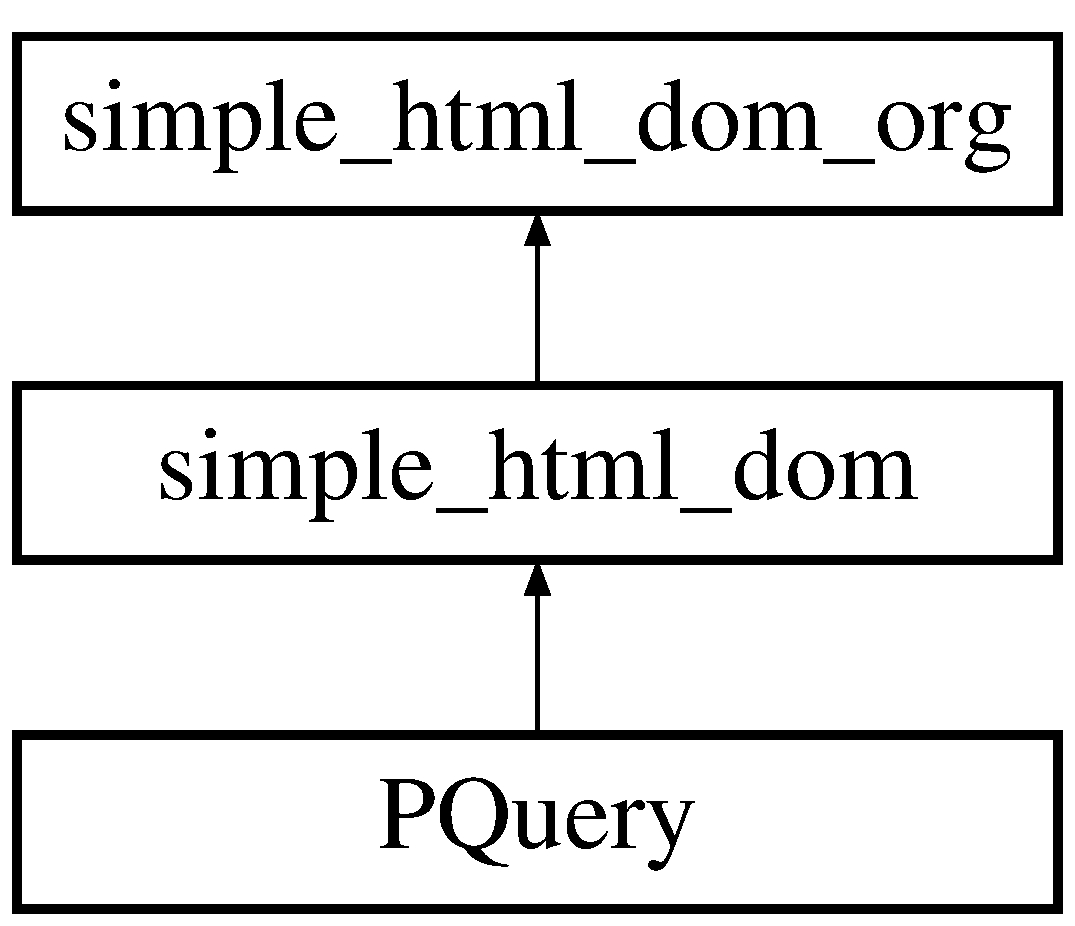
\includegraphics[height=3.000000cm]{class_p_query}
\end{center}
\end{figure}
\subsection*{公開メンバ関数}
\begin{DoxyCompactItemize}
\item 
\hypertarget{class_p_query_a6d032ac38c617a86c7e8e6b40b8fd7ed}{}{\bfseries \+\_\+\+\_\+construct} (\$arg\+Target, \$arg\+String\+Enabled=N\+U\+L\+L, \$arg\+File\+Encoding=N\+U\+L\+L, \$arg\+Convert\+Encoding=N\+U\+L\+L)\label{class_p_query_a6d032ac38c617a86c7e8e6b40b8fd7ed}

\item 
\hyperlink{class_p_query_a9a4359416363f682c92fda62c43babda}{add\+Source} (\$arg\+Hint, \$arg\+Target, \$arg\+File\+Encoding=N\+U\+L\+L, \$arg\+Convert\+Encoding=N\+U\+L\+L, \$arg\+Outer\+Enabled=F\+A\+L\+S\+E)
\item 
\hyperlink{class_p_query_a276c00b5befedae7349d0945f5d6ba28}{refresh} ()
\item 
\hyperlink{class_p_query_acd073383bc3c77f25fc52d1caa7389a9}{flush} ()
\item 
\hyperlink{class_p_query_aa9307a2df5e2c760c7b15fb2ad7e2fbd}{assign\+Text} (\$arg\+Nodes, \$arg\+Text, \$arg\+Outer\+Enabled=F\+A\+L\+S\+E)
\item 
\hyperlink{class_p_query_a14104b2c5b7368417e81539d9c571693}{assign\+Html} (\$arg\+Nodes, \$arg\+Text, \$arg\+Outer\+Enabled=F\+A\+L\+S\+E)
\item 
\hyperlink{class_p_query_a37cb8439c38a831553457b3ce7c8846a}{put} (\$arg\+Target, \$arg\+Value)
\item 
\hyperlink{class_p_query_a09255b571a9b0aade9de1acbe0850864}{set\+Form} (\$argumets)
\item 
\hyperlink{class_p_query_a25f666ee0150463eced87debad60ef93}{get\+Attr} (\$arg\+Target, \$arg\+Target\+Attr)
\item 
\hyperlink{class_p_query_a34ad0dca40dd24dea9f88c608a5cb149}{set\+Attr} (\$arg\+Target, \$arg\+Target\+Attr, \$arg\+Value)
\end{DoxyCompactItemize}
\subsection*{静的限定公開メンバ関数}
\begin{DoxyCompactItemize}
\item 
\hypertarget{class_p_query_a83a101c5c6d7e1ffd66ed393344d5019}{}static \& {\bfseries \+\_\+convert\+Buffer} (\&\$arg\+Buffer, \$arg\+File\+Encoding=N\+U\+L\+L, \$arg\+Convert\+Encoding=N\+U\+L\+L)\label{class_p_query_a83a101c5c6d7e1ffd66ed393344d5019}

\item 
\hypertarget{class_p_query_a78cc4ef8d21c02797bfe69140be7a6f1}{}static \& {\bfseries \+\_\+read\+Buffer} (\$arg\+Target, \$arg\+String\+Enabled=N\+U\+L\+L, \$arg\+File\+Encoding=N\+U\+L\+L, \$arg\+Convert\+Encoding=N\+U\+L\+L)\label{class_p_query_a78cc4ef8d21c02797bfe69140be7a6f1}

\end{DoxyCompactItemize}


\subsection{詳解}
J\+Queryを真似した、simple\+\_\+html\+\_\+domを利用した\+Selector P\+Queryの\+Pは\+P\+H\+Pの\+P X\+M\+Lないし\+Htmlを\+Selectorでごにょごにょするクラス 

\subsection{関数詳解}
\hypertarget{class_p_query_a9a4359416363f682c92fda62c43babda}{}\index{P\+Query@{P\+Query}!add\+Source@{add\+Source}}
\index{add\+Source@{add\+Source}!P\+Query@{P\+Query}}
\subsubsection[{add\+Source}]{\setlength{\rightskip}{0pt plus 5cm}P\+Query\+::add\+Source (
\begin{DoxyParamCaption}
\item[{}]{\$arg\+Hint, }
\item[{}]{\$arg\+Target, }
\item[{}]{\$arg\+File\+Encoding = {\ttfamily NULL}, }
\item[{}]{\$arg\+Convert\+Encoding = {\ttfamily NULL}, }
\item[{}]{\$arg\+Outer\+Enabled = {\ttfamily FALSE}}
\end{DoxyParamCaption}
)}\label{class_p_query_a9a4359416363f682c92fda62c43babda}
ソースを追加する \hypertarget{class_p_query_a14104b2c5b7368417e81539d9c571693}{}\index{P\+Query@{P\+Query}!assign\+Html@{assign\+Html}}
\index{assign\+Html@{assign\+Html}!P\+Query@{P\+Query}}
\subsubsection[{assign\+Html}]{\setlength{\rightskip}{0pt plus 5cm}P\+Query\+::assign\+Html (
\begin{DoxyParamCaption}
\item[{}]{\$arg\+Nodes, }
\item[{}]{\$arg\+Text, }
\item[{}]{\$arg\+Outer\+Enabled = {\ttfamily FALSE}}
\end{DoxyParamCaption}
)}\label{class_p_query_a14104b2c5b7368417e81539d9c571693}
該当htmlノードの一括置換 \hypertarget{class_p_query_aa9307a2df5e2c760c7b15fb2ad7e2fbd}{}\index{P\+Query@{P\+Query}!assign\+Text@{assign\+Text}}
\index{assign\+Text@{assign\+Text}!P\+Query@{P\+Query}}
\subsubsection[{assign\+Text}]{\setlength{\rightskip}{0pt plus 5cm}P\+Query\+::assign\+Text (
\begin{DoxyParamCaption}
\item[{}]{\$arg\+Nodes, }
\item[{}]{\$arg\+Text, }
\item[{}]{\$arg\+Outer\+Enabled = {\ttfamily FALSE}}
\end{DoxyParamCaption}
)}\label{class_p_query_aa9307a2df5e2c760c7b15fb2ad7e2fbd}
該当textノードの一括置換 \hypertarget{class_p_query_acd073383bc3c77f25fc52d1caa7389a9}{}\index{P\+Query@{P\+Query}!flush@{flush}}
\index{flush@{flush}!P\+Query@{P\+Query}}
\subsubsection[{flush}]{\setlength{\rightskip}{0pt plus 5cm}P\+Query\+::flush (
\begin{DoxyParamCaption}
{}
\end{DoxyParamCaption}
)}\label{class_p_query_acd073383bc3c77f25fc52d1caa7389a9}
html文字列にして返却 \hypertarget{class_p_query_a25f666ee0150463eced87debad60ef93}{}\index{P\+Query@{P\+Query}!get\+Attr@{get\+Attr}}
\index{get\+Attr@{get\+Attr}!P\+Query@{P\+Query}}
\subsubsection[{get\+Attr}]{\setlength{\rightskip}{0pt plus 5cm}P\+Query\+::get\+Attr (
\begin{DoxyParamCaption}
\item[{}]{\$arg\+Target, }
\item[{}]{\$arg\+Target\+Attr}
\end{DoxyParamCaption}
)}\label{class_p_query_a25f666ee0150463eced87debad60ef93}
set\+Attributeまでの処理をラップして簡単にしたもの \hypertarget{class_p_query_a37cb8439c38a831553457b3ce7c8846a}{}\index{P\+Query@{P\+Query}!put@{put}}
\index{put@{put}!P\+Query@{P\+Query}}
\subsubsection[{put}]{\setlength{\rightskip}{0pt plus 5cm}P\+Query\+::put (
\begin{DoxyParamCaption}
\item[{}]{\$arg\+Target, }
\item[{}]{\$arg\+Value}
\end{DoxyParamCaption}
)}\label{class_p_query_a37cb8439c38a831553457b3ce7c8846a}
dom\+Stoneを作って保持する assignまでの処理をラップして簡単にしたもの \hypertarget{class_p_query_a276c00b5befedae7349d0945f5d6ba28}{}\index{P\+Query@{P\+Query}!refresh@{refresh}}
\index{refresh@{refresh}!P\+Query@{P\+Query}}
\subsubsection[{refresh}]{\setlength{\rightskip}{0pt plus 5cm}P\+Query\+::refresh (
\begin{DoxyParamCaption}
{}
\end{DoxyParamCaption}
)}\label{class_p_query_a276c00b5befedae7349d0945f5d6ba28}
パースし直し \hypertarget{class_p_query_a34ad0dca40dd24dea9f88c608a5cb149}{}\index{P\+Query@{P\+Query}!set\+Attr@{set\+Attr}}
\index{set\+Attr@{set\+Attr}!P\+Query@{P\+Query}}
\subsubsection[{set\+Attr}]{\setlength{\rightskip}{0pt plus 5cm}P\+Query\+::set\+Attr (
\begin{DoxyParamCaption}
\item[{}]{\$arg\+Target, }
\item[{}]{\$arg\+Target\+Attr, }
\item[{}]{\$arg\+Value}
\end{DoxyParamCaption}
)}\label{class_p_query_a34ad0dca40dd24dea9f88c608a5cb149}
set\+Attributeまでの処理をラップして簡単にしたもの \hypertarget{class_p_query_a09255b571a9b0aade9de1acbe0850864}{}\index{P\+Query@{P\+Query}!set\+Form@{set\+Form}}
\index{set\+Form@{set\+Form}!P\+Query@{P\+Query}}
\subsubsection[{set\+Form}]{\setlength{\rightskip}{0pt plus 5cm}P\+Query\+::set\+Form (
\begin{DoxyParamCaption}
\item[{}]{\$argumets}
\end{DoxyParamCaption}
)}\label{class_p_query_a09255b571a9b0aade9de1acbe0850864}
form値セットを簡単にしたもの X\+X\+X コレを利用したい場合は自動セットさせたいformのネームをテンプレートファイルのベースネームと一致させて置くこと! 

このクラス詳解は次のファイルから抽出されました\+:\begin{DoxyCompactItemize}
\item 
Generic\+Package/class/\+Template\+Engine/P\+Query.\+class.\+php\end{DoxyCompactItemize}

\hypertarget{class_rest}{}\section{Rest クラス}
\label{class_rest}\index{Rest@{Rest}}
Rest の継承関係図\begin{figure}[H]
\begin{center}
\leavevmode
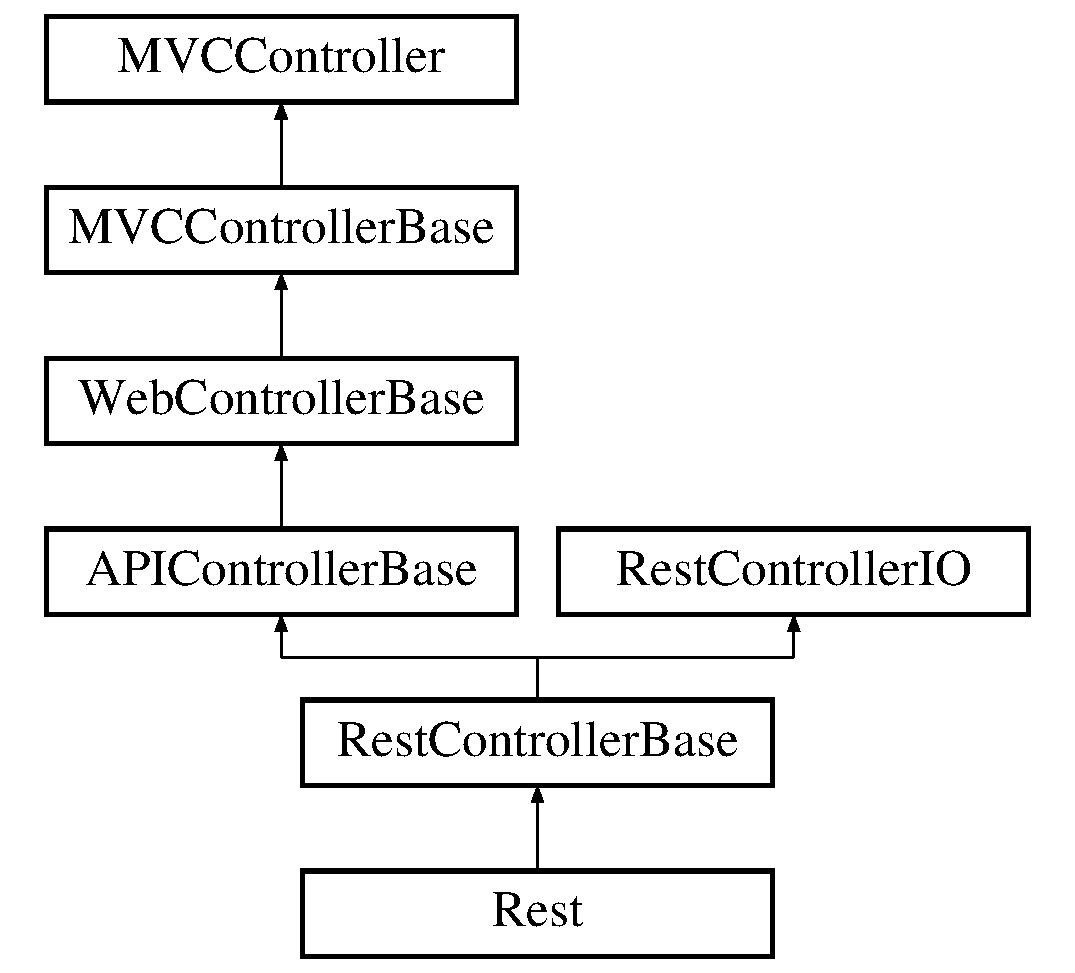
\includegraphics[height=6.000000cm]{class_rest}
\end{center}
\end{figure}
\subsection*{公開メンバ関数}
\begin{DoxyCompactItemize}
\item 
\hyperlink{class_rest_a6b69aeaec7507e4544cf13cfe402a7cb}{get} ()
\item 
\hyperlink{class_rest_aadf4ba482ce65d9423b6ce904695b50c}{post} (\$arg\+Request\+Params=N\+U\+L\+L)
\item 
\hyperlink{class_rest_a7e73d86dc864a3686ca192a32355bc02}{put} (\$arg\+Request\+Params=N\+U\+L\+L)
\item 
\hyperlink{class_rest_ad7d643a90903bc310129f8c5371ae9b3}{delete} ()
\item 
\hyperlink{class_rest_a0a60cc099ed9a1b70fa45b7c18f2c228}{head} ()
\end{DoxyCompactItemize}
\subsection*{その他の継承メンバ}


\subsection{関数詳解}
\hypertarget{class_rest_ad7d643a90903bc310129f8c5371ae9b3}{}\index{Rest@{Rest}!delete@{delete}}
\index{delete@{delete}!Rest@{Rest}}
\subsubsection[{delete}]{\setlength{\rightskip}{0pt plus 5cm}Rest\+::delete (
\begin{DoxyParamCaption}
{}
\end{DoxyParamCaption}
)}\label{class_rest_ad7d643a90903bc310129f8c5371ae9b3}
リソースの削除 \begin{DoxyReturn}{戻り値}
boolean 
\end{DoxyReturn}


\hyperlink{interface_rest_controller_i_o_aea37c094d38f5c7ff6b5a52e9f4f30a6}{Rest\+Controller\+I\+O}を実装しています。

\hypertarget{class_rest_a6b69aeaec7507e4544cf13cfe402a7cb}{}\index{Rest@{Rest}!get@{get}}
\index{get@{get}!Rest@{Rest}}
\subsubsection[{get}]{\setlength{\rightskip}{0pt plus 5cm}Rest\+::get (
\begin{DoxyParamCaption}
{}
\end{DoxyParamCaption}
)}\label{class_rest_a6b69aeaec7507e4544cf13cfe402a7cb}
リソースの参照 \begin{DoxyReturn}{戻り値}
mixed 成功時は最新のリソース配列 失敗時は\+F\+A\+L\+S\+E 
\end{DoxyReturn}


\hyperlink{interface_rest_controller_i_o_af268b91d81734f22569982048ae81a1f}{Rest\+Controller\+I\+O}を実装しています。

\hypertarget{class_rest_a0a60cc099ed9a1b70fa45b7c18f2c228}{}\index{Rest@{Rest}!head@{head}}
\index{head@{head}!Rest@{Rest}}
\subsubsection[{head}]{\setlength{\rightskip}{0pt plus 5cm}Rest\+::head (
\begin{DoxyParamCaption}
{}
\end{DoxyParamCaption}
)}\label{class_rest_a0a60cc099ed9a1b70fa45b7c18f2c228}
リソースの情報の取得 \begin{DoxyReturn}{戻り値}
boolean 
\end{DoxyReturn}
\hypertarget{class_rest_aadf4ba482ce65d9423b6ce904695b50c}{}\index{Rest@{Rest}!post@{post}}
\index{post@{post}!Rest@{Rest}}
\subsubsection[{post}]{\setlength{\rightskip}{0pt plus 5cm}Rest\+::post (
\begin{DoxyParamCaption}
\item[{}]{\$arg\+Request\+Params = {\ttfamily NULL}}
\end{DoxyParamCaption}
)}\label{class_rest_aadf4ba482ce65d9423b6ce904695b50c}
リソースの作成・更新・インクリメント・デクリメント \begin{DoxyReturn}{戻り値}
mixed 成功時は最新のリソース配列 失敗時は\+F\+A\+L\+S\+E 
\end{DoxyReturn}
\hypertarget{class_rest_a7e73d86dc864a3686ca192a32355bc02}{}\index{Rest@{Rest}!put@{put}}
\index{put@{put}!Rest@{Rest}}
\subsubsection[{put}]{\setlength{\rightskip}{0pt plus 5cm}Rest\+::put (
\begin{DoxyParamCaption}
\item[{}]{\$arg\+Request\+Params = {\ttfamily NULL}}
\end{DoxyParamCaption}
)}\label{class_rest_a7e73d86dc864a3686ca192a32355bc02}
リソースの作成・更新 \begin{DoxyReturn}{戻り値}
mixed 成功時は最新のリソース配列 失敗時は\+F\+A\+L\+S\+E 
\end{DoxyReturn}


このクラス詳解は次のファイルから抽出されました\+:\begin{DoxyCompactItemize}
\item 
Framework\+Package/class/\+M\+V\+C/\+Controller/Rest.\+php\end{DoxyCompactItemize}

\hypertarget{class_rest_controller_base}{}\section{Rest\+Controller\+Base クラス}
\label{class_rest_controller_base}\index{Rest\+Controller\+Base@{Rest\+Controller\+Base}}
Rest\+Controller\+Base の継承関係図\begin{figure}[H]
\begin{center}
\leavevmode
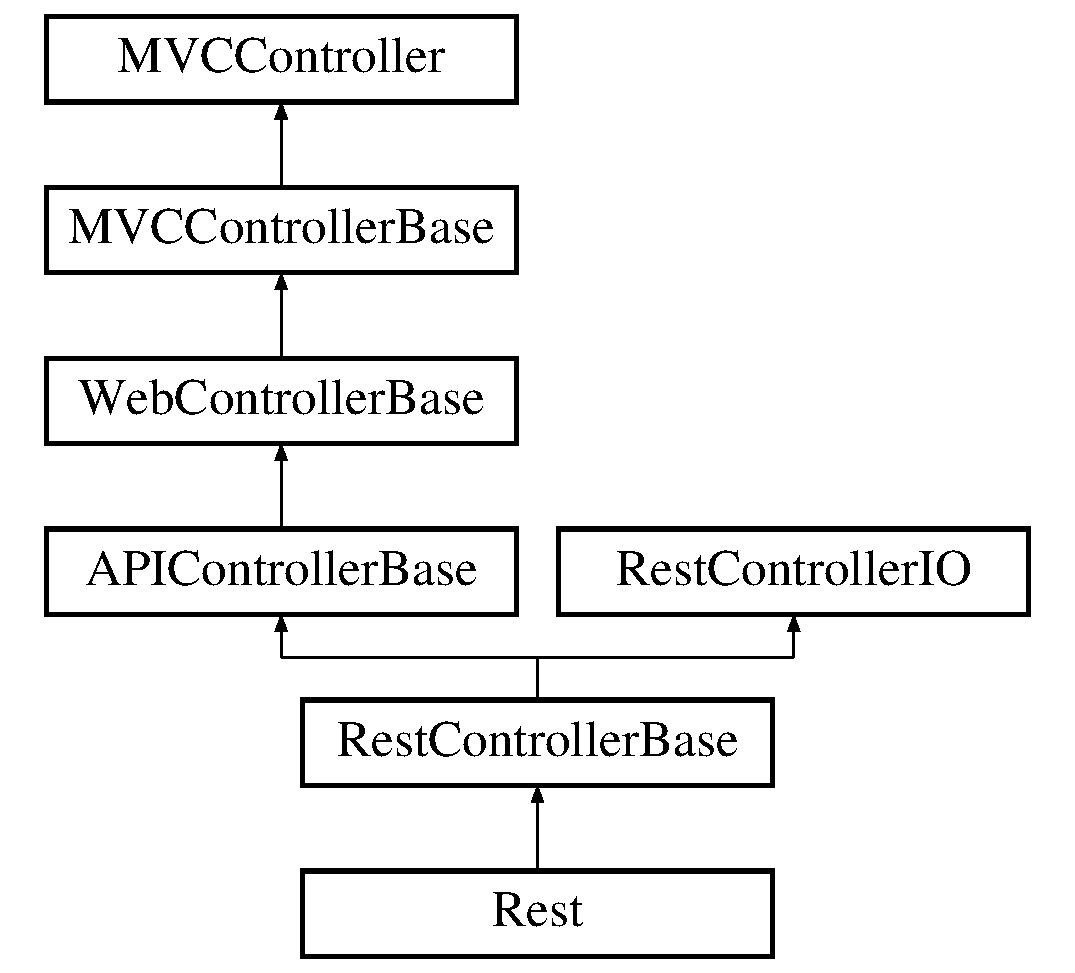
\includegraphics[height=6.000000cm]{class_rest_controller_base}
\end{center}
\end{figure}
\subsection*{公開メンバ関数}
\begin{DoxyCompactItemize}
\item 
\hypertarget{class_rest_controller_base_a26a400c6a6547ff09c8badcbe62af52a}{}{\bfseries get\+D\+B\+O} (\$arg\+D\+S\+N=N\+U\+L\+L)\label{class_rest_controller_base_a26a400c6a6547ff09c8badcbe62af52a}

\item 
\hypertarget{class_rest_controller_base_a7a2a49f6743241f8cbaaddb08bcc4c2b}{}{\bfseries get\+Model} (\$arg\+Model, \$arg\+Identifier\+O\+R\+Query=N\+U\+L\+L, \$arg\+Binds=N\+U\+L\+L, \$arg\+D\+S\+N=N\+U\+L\+L)\label{class_rest_controller_base_a7a2a49f6743241f8cbaaddb08bcc4c2b}

\item 
\hypertarget{class_rest_controller_base_a59b19c50ca7006f746d91d7237018e01}{}{\bfseries convert\+Array\+From\+Model} (\$Arg\+Model, \$arg\+Fields=N\+U\+L\+L)\label{class_rest_controller_base_a59b19c50ca7006f746d91d7237018e01}

\item 
\hypertarget{class_rest_controller_base_a95ad94f5d58231686aea32c58749175c}{}{\bfseries get\+Request\+Params} ()\label{class_rest_controller_base_a95ad94f5d58231686aea32c58749175c}

\item 
\hyperlink{class_rest_controller_base_a648e6ebeaef466e01e6281c1178d2cc0}{U\+I\+D\+Auth\+And\+Execute} ()
\item 
\hyperlink{class_rest_controller_base_ae3e9e4f549693f6b28edd415e9b38747}{auth\+And\+Execute} ()
\item 
\hyperlink{class_rest_controller_base_aba28a2fce30920ac9e816d6dde7f8d2f}{execute} (\$arg\+Resource\+Hint=N\+U\+L\+L, \$arg\+Request\+Params=N\+U\+L\+L)
\item 
\hyperlink{class_rest_controller_base_a842a9ecef6680268e367a44c4df951a2}{get} ()
\item 
\hyperlink{class_rest_controller_base_a305d42e434b069c7c7e5916f2c46682a}{post} (\$arg\+Request\+Params=N\+U\+L\+L)
\item 
\hyperlink{class_rest_controller_base_a95556be57cfc461f8703f0f369ee05d5}{put} (\$arg\+Request\+Params=N\+U\+L\+L)
\item 
\hyperlink{class_rest_controller_base_a1a30a132626984159384c227f5cdc717}{delete} ()
\item 
\hyperlink{class_rest_controller_base_adbae680f95aaf268f9673790fb592d3c}{head} ()
\end{DoxyCompactItemize}
\subsection*{静的公開メンバ関数}
\begin{DoxyCompactItemize}
\item 
\hypertarget{class_rest_controller_base_a95adbcb37b5e2800c40fbb58c99d5725}{}static {\bfseries resolve\+Request\+Params} ()\label{class_rest_controller_base_a95adbcb37b5e2800c40fbb58c99d5725}

\item 
static \hyperlink{class_rest_controller_base_af58b2d2698c8cca84d6d7c346aaabfba}{resolve\+R\+E\+S\+T\+Resource} (\$arg\+R\+E\+S\+T\+Resource\+Hint)
\end{DoxyCompactItemize}
\subsection*{公開変数類}
\begin{DoxyCompactItemize}
\item 
\hypertarget{class_rest_controller_base_a6f393be69d966a891945ef2b3867ab43}{}{\bfseries \$request\+Method} = \textquotesingle{}G\+E\+T\textquotesingle{}\label{class_rest_controller_base_a6f393be69d966a891945ef2b3867ab43}

\item 
\hypertarget{class_rest_controller_base_a0a6f69ab785a9898ecc69fecc823c39f}{}{\bfseries \$rest\+Resource} = \textquotesingle{}\textquotesingle{}\label{class_rest_controller_base_a0a6f69ab785a9898ecc69fecc823c39f}

\item 
\hypertarget{class_rest_controller_base_a6b85ac821de6d00fc424dfd00b38f0b1}{}{\bfseries \$rest\+Resource\+Model} = \textquotesingle{}\textquotesingle{}\label{class_rest_controller_base_a6b85ac821de6d00fc424dfd00b38f0b1}

\item 
\hypertarget{class_rest_controller_base_a30307dce16a06ef455a287c41c7600f2}{}{\bfseries \$rest\+Resource\+Listed} = N\+U\+L\+L\label{class_rest_controller_base_a30307dce16a06ef455a287c41c7600f2}

\item 
\hypertarget{class_rest_controller_base_afc035b4462634549407ef97b4e69f733}{}{\bfseries \$rest\+Resource\+Create\+Date\+Key\+Name} = \textquotesingle{}\textquotesingle{}\label{class_rest_controller_base_afc035b4462634549407ef97b4e69f733}

\item 
\hypertarget{class_rest_controller_base_ae6b9ea774a33e6806a482cf73a1434f8}{}{\bfseries \$rest\+Resource\+Modify\+Date\+Key\+Name} = \textquotesingle{}\textquotesingle{}\label{class_rest_controller_base_ae6b9ea774a33e6806a482cf73a1434f8}

\item 
\hypertarget{class_rest_controller_base_a11364ff92cfd143a980659ee6a6eaf43}{}{\bfseries \$rest\+Resource\+Available\+Key\+Name} = \textquotesingle{}\textquotesingle{}\label{class_rest_controller_base_a11364ff92cfd143a980659ee6a6eaf43}

\item 
\hypertarget{class_rest_controller_base_a066ee8c6a20f8c126fb6a0cdd5776b01}{}{\bfseries \$rest\+Resource\+User\+Table\+Name} = N\+U\+L\+L\label{class_rest_controller_base_a066ee8c6a20f8c126fb6a0cdd5776b01}

\item 
\hypertarget{class_rest_controller_base_aaac5c04431d48b5c123666eb2f68fd00}{}{\bfseries \$rest\+Resource\+Relay\+Suffix} = \textquotesingle{}\textquotesingle{}\label{class_rest_controller_base_aaac5c04431d48b5c123666eb2f68fd00}

\item 
\hypertarget{class_rest_controller_base_a6b6690a161550e7ca4fd98c5b42c9653}{}{\bfseries \$rest\+Resource\+Relay\+Prefix} = \textquotesingle{}\textquotesingle{}\label{class_rest_controller_base_a6b6690a161550e7ca4fd98c5b42c9653}

\item 
\hypertarget{class_rest_controller_base_a7ac3e3dc294f8148f382b642fe189b73}{}{\bfseries \$\+Auth\+Device} = N\+U\+L\+L\label{class_rest_controller_base_a7ac3e3dc294f8148f382b642fe189b73}

\item 
\hypertarget{class_rest_controller_base_aff05f64025725b1bcd83fd344ea2a1ac}{}{\bfseries \$\+Auth\+User} = N\+U\+L\+L\label{class_rest_controller_base_aff05f64025725b1bcd83fd344ea2a1ac}

\item 
\hypertarget{class_rest_controller_base_a22e2c927f7df24f55851593cee338811}{}{\bfseries \$auth\+User\+I\+D} = N\+U\+L\+L\label{class_rest_controller_base_a22e2c927f7df24f55851593cee338811}

\item 
\hypertarget{class_rest_controller_base_aca6c6c8637ebe32a99e70d16394255d7}{}{\bfseries \$auth\+User\+I\+D\+Field\+Name} = N\+U\+L\+L\label{class_rest_controller_base_aca6c6c8637ebe32a99e70d16394255d7}

\item 
\hypertarget{class_rest_controller_base_ac16e13138b6ac9fd8245b094ae287bc1}{}{\bfseries \$auth\+User\+Query} = N\+U\+L\+L\label{class_rest_controller_base_ac16e13138b6ac9fd8245b094ae287bc1}

\item 
\hypertarget{class_rest_controller_base_a743204aa1d9057972a308ffcc070f742}{}{\bfseries \$deep\+R\+E\+S\+T\+Mode} = T\+R\+U\+E\label{class_rest_controller_base_a743204aa1d9057972a308ffcc070f742}

\item 
\hypertarget{class_rest_controller_base_abd5722b94c46ec8a9330eb24e8105f82}{}{\bfseries \$root\+R\+E\+S\+T} = T\+R\+U\+E\label{class_rest_controller_base_abd5722b94c46ec8a9330eb24e8105f82}

\item 
\hypertarget{class_rest_controller_base_ab06c4e2e087706ee21b5c3a7c1452ac8}{}{\bfseries \$virtual\+R\+E\+S\+T} = F\+A\+L\+S\+E\label{class_rest_controller_base_ab06c4e2e087706ee21b5c3a7c1452ac8}

\item 
\hypertarget{class_rest_controller_base_a2f460e29265d4f811f93d6554c894ee3}{}{\bfseries \$responce\+Data} = F\+A\+L\+S\+E\label{class_rest_controller_base_a2f460e29265d4f811f93d6554c894ee3}

\end{DoxyCompactItemize}
\subsection*{静的公開変数類}
\begin{DoxyCompactItemize}
\item 
\hypertarget{class_rest_controller_base_a89efa2069bb58cdb9d2d8c215ca7026f}{}static {\bfseries \$now\+G\+M\+T} = N\+U\+L\+L\label{class_rest_controller_base_a89efa2069bb58cdb9d2d8c215ca7026f}

\end{DoxyCompactItemize}
\subsection*{限定公開メンバ関数}
\begin{DoxyCompactItemize}
\item 
\hypertarget{class_rest_controller_base_a698e344e2c6f158a37defa29015dc05d}{}{\bfseries \+\_\+init} ()\label{class_rest_controller_base_a698e344e2c6f158a37defa29015dc05d}

\item 
\hypertarget{class_rest_controller_base_af8b8730ca0146b74caeeb0bd302fdee0}{}{\bfseries \+\_\+get\+Model} (\$arg\+Model, \$arg\+Identifier\+O\+R\+Query=N\+U\+L\+L, \$arg\+Binds=N\+U\+L\+L, \$arg\+D\+S\+N=N\+U\+L\+L)\label{class_rest_controller_base_af8b8730ca0146b74caeeb0bd302fdee0}

\item 
\hypertarget{class_rest_controller_base_a94426891fdd91eafa514539524514056}{}{\bfseries \+\_\+convert\+Array\+From\+Model} (\$Arg\+Model, \$arg\+Fields=N\+U\+L\+L)\label{class_rest_controller_base_a94426891fdd91eafa514539524514056}

\end{DoxyCompactItemize}
\subsection*{静的限定公開メンバ関数}
\begin{DoxyCompactItemize}
\item 
\hypertarget{class_rest_controller_base_a87e1a761d90332ddff422cefe3f65b16}{}static {\bfseries \+\_\+get\+D\+B\+O} (\$arg\+D\+S\+N=N\+U\+L\+L)\label{class_rest_controller_base_a87e1a761d90332ddff422cefe3f65b16}

\end{DoxyCompactItemize}
\subsection*{限定公開変数類}
\begin{DoxyCompactItemize}
\item 
\hypertarget{class_rest_controller_base_a1cc144075c95012b24a82aa964ded88c}{}{\bfseries \$\+\_\+initialized} = F\+A\+L\+S\+E\label{class_rest_controller_base_a1cc144075c95012b24a82aa964ded88c}

\end{DoxyCompactItemize}


\subsection{関数詳解}
\hypertarget{class_rest_controller_base_ae3e9e4f549693f6b28edd415e9b38747}{}\index{Rest\+Controller\+Base@{Rest\+Controller\+Base}!auth\+And\+Execute@{auth\+And\+Execute}}
\index{auth\+And\+Execute@{auth\+And\+Execute}!Rest\+Controller\+Base@{Rest\+Controller\+Base}}
\subsubsection[{auth\+And\+Execute}]{\setlength{\rightskip}{0pt plus 5cm}Rest\+Controller\+Base\+::auth\+And\+Execute (
\begin{DoxyParamCaption}
{}
\end{DoxyParamCaption}
)}\label{class_rest_controller_base_ae3e9e4f549693f6b28edd415e9b38747}
フレームワーク標準の\+Auth機能を利用した認証を行って、\+R\+E\+S\+Tする \begin{DoxyReturn}{戻り値}
array 配列構造のリソースデータ 
\end{DoxyReturn}
\hypertarget{class_rest_controller_base_a1a30a132626984159384c227f5cdc717}{}\index{Rest\+Controller\+Base@{Rest\+Controller\+Base}!delete@{delete}}
\index{delete@{delete}!Rest\+Controller\+Base@{Rest\+Controller\+Base}}
\subsubsection[{delete}]{\setlength{\rightskip}{0pt plus 5cm}Rest\+Controller\+Base\+::delete (
\begin{DoxyParamCaption}
{}
\end{DoxyParamCaption}
)}\label{class_rest_controller_base_a1a30a132626984159384c227f5cdc717}
D\+E\+L\+E\+T\+Eメソッド X\+X\+X モデルの位置付けが、テーブルリソースで無い場合は、継承して\+R\+E\+S\+Tの”冪等性”に従って実装して下さい(冪等性を持ちます) \begin{DoxyReturn}{戻り値}
boolean 
\end{DoxyReturn}


\hyperlink{interface_rest_controller_i_o_aea37c094d38f5c7ff6b5a52e9f4f30a6}{Rest\+Controller\+I\+O}を実装しています。

\hypertarget{class_rest_controller_base_aba28a2fce30920ac9e816d6dde7f8d2f}{}\index{Rest\+Controller\+Base@{Rest\+Controller\+Base}!execute@{execute}}
\index{execute@{execute}!Rest\+Controller\+Base@{Rest\+Controller\+Base}}
\subsubsection[{execute}]{\setlength{\rightskip}{0pt plus 5cm}Rest\+Controller\+Base\+::execute (
\begin{DoxyParamCaption}
\item[{}]{\$arg\+Resource\+Hint = {\ttfamily NULL}, }
\item[{}]{\$arg\+Request\+Params = {\ttfamily NULL}}
\end{DoxyParamCaption}
)}\label{class_rest_controller_base_aba28a2fce30920ac9e816d6dde7f8d2f}
R\+E\+S\+Tする \begin{DoxyReturn}{戻り値}
array 配列構造のリソースデータ 
\end{DoxyReturn}
\hypertarget{class_rest_controller_base_a842a9ecef6680268e367a44c4df951a2}{}\index{Rest\+Controller\+Base@{Rest\+Controller\+Base}!get@{get}}
\index{get@{get}!Rest\+Controller\+Base@{Rest\+Controller\+Base}}
\subsubsection[{get}]{\setlength{\rightskip}{0pt plus 5cm}Rest\+Controller\+Base\+::get (
\begin{DoxyParamCaption}
{}
\end{DoxyParamCaption}
)}\label{class_rest_controller_base_a842a9ecef6680268e367a44c4df951a2}
G\+E\+Tメソッド リソースの参照(冪等性を持ちます) X\+X\+X モデルの位置付けが、テーブルリソースで無い場合は、継承して、\+R\+E\+S\+Tの”冪等性”に従って実装して下さい \begin{DoxyReturn}{戻り値}
mixed 成功時は最新のリソース配列 失敗時は\+F\+A\+L\+S\+E 
\end{DoxyReturn}


\hyperlink{interface_rest_controller_i_o_af268b91d81734f22569982048ae81a1f}{Rest\+Controller\+I\+O}を実装しています。

\hypertarget{class_rest_controller_base_adbae680f95aaf268f9673790fb592d3c}{}\index{Rest\+Controller\+Base@{Rest\+Controller\+Base}!head@{head}}
\index{head@{head}!Rest\+Controller\+Base@{Rest\+Controller\+Base}}
\subsubsection[{head}]{\setlength{\rightskip}{0pt plus 5cm}Rest\+Controller\+Base\+::head (
\begin{DoxyParamCaption}
{}
\end{DoxyParamCaption}
)}\label{class_rest_controller_base_adbae680f95aaf268f9673790fb592d3c}
H\+E\+A\+Dメソッド \begin{DoxyReturn}{戻り値}
boolean 
\end{DoxyReturn}
\hypertarget{class_rest_controller_base_a305d42e434b069c7c7e5916f2c46682a}{}\index{Rest\+Controller\+Base@{Rest\+Controller\+Base}!post@{post}}
\index{post@{post}!Rest\+Controller\+Base@{Rest\+Controller\+Base}}
\subsubsection[{post}]{\setlength{\rightskip}{0pt plus 5cm}Rest\+Controller\+Base\+::post (
\begin{DoxyParamCaption}
\item[{}]{\$arg\+Request\+Params = {\ttfamily NULL}}
\end{DoxyParamCaption}
)}\label{class_rest_controller_base_a305d42e434b069c7c7e5916f2c46682a}
P\+O\+S\+Tメソッド リソースの新規作成、更新、インクリメント、デクリメント(冪等性を強制しません) X\+X\+X モデルの位置付けが、テーブルリソースで無い場合は、継承して、\+R\+E\+S\+Tの”冪等性”に従って実装して下さい \begin{DoxyReturn}{戻り値}
mixed 成功時は最新のリソース配列 失敗時は\+F\+A\+L\+S\+E 
\end{DoxyReturn}
\hypertarget{class_rest_controller_base_a95556be57cfc461f8703f0f369ee05d5}{}\index{Rest\+Controller\+Base@{Rest\+Controller\+Base}!put@{put}}
\index{put@{put}!Rest\+Controller\+Base@{Rest\+Controller\+Base}}
\subsubsection[{put}]{\setlength{\rightskip}{0pt plus 5cm}Rest\+Controller\+Base\+::put (
\begin{DoxyParamCaption}
\item[{}]{\$arg\+Request\+Params = {\ttfamily NULL}}
\end{DoxyParamCaption}
)}\label{class_rest_controller_base_a95556be57cfc461f8703f0f369ee05d5}
P\+U\+Tメソッド リソースの新規作成、更新(冪等性を持ちます) X\+X\+X モデルの位置付けが、テーブルリソースで無い場合は、継承して、\+R\+E\+S\+Tの”冪等性”に従って実装して下さい \begin{DoxyReturn}{戻り値}
mixed 成功時は最新のリソース配列 失敗時は\+F\+A\+L\+S\+E 
\end{DoxyReturn}
\hypertarget{class_rest_controller_base_af58b2d2698c8cca84d6d7c346aaabfba}{}\index{Rest\+Controller\+Base@{Rest\+Controller\+Base}!resolve\+R\+E\+S\+T\+Resource@{resolve\+R\+E\+S\+T\+Resource}}
\index{resolve\+R\+E\+S\+T\+Resource@{resolve\+R\+E\+S\+T\+Resource}!Rest\+Controller\+Base@{Rest\+Controller\+Base}}
\subsubsection[{resolve\+R\+E\+S\+T\+Resource}]{\setlength{\rightskip}{0pt plus 5cm}static Rest\+Controller\+Base\+::resolve\+R\+E\+S\+T\+Resource (
\begin{DoxyParamCaption}
\item[{}]{\$arg\+R\+E\+S\+T\+Resource\+Hint}
\end{DoxyParamCaption}
)\hspace{0.3cm}{\ttfamily [static]}}\label{class_rest_controller_base_af58b2d2698c8cca84d6d7c346aaabfba}
R\+E\+S\+T\+A\+P\+Iでリソースにアクセスする際の指定リソース情報を分解してパラメータ化します \mbox{[}me指定(任意)/\mbox{]}\mbox{[}model指定(必須)/\mbox{]}\mbox{[}pkey指定(,pkey指定,...)(G\+E\+T以外は必須)/\mbox{]} 例) 自分の\char`\"{}model\char`\"{}の一覧を取得 /me/model.json X\+X\+X システム毎に\+R\+E\+S\+Tの\+U\+R\+Iパラメータ分解法が違う場合はこのメソッドをオーバーライドして下さい 
\begin{DoxyParams}[1]{引数}
string & {\em \$arg\+R\+E\+S\+T\+Resource\+Hint} & \\
\hline
\end{DoxyParams}
\begin{DoxyReturn}{戻り値}
array model,listed,fields,idsの配列 
\end{DoxyReturn}
\hypertarget{class_rest_controller_base_a648e6ebeaef466e01e6281c1178d2cc0}{}\index{Rest\+Controller\+Base@{Rest\+Controller\+Base}!U\+I\+D\+Auth\+And\+Execute@{U\+I\+D\+Auth\+And\+Execute}}
\index{U\+I\+D\+Auth\+And\+Execute@{U\+I\+D\+Auth\+And\+Execute}!Rest\+Controller\+Base@{Rest\+Controller\+Base}}
\subsubsection[{U\+I\+D\+Auth\+And\+Execute}]{\setlength{\rightskip}{0pt plus 5cm}Rest\+Controller\+Base\+::\+U\+I\+D\+Auth\+And\+Execute (
\begin{DoxyParamCaption}
{}
\end{DoxyParamCaption}
)}\label{class_rest_controller_base_a648e6ebeaef466e01e6281c1178d2cc0}
フレームワーク標準の\+Auth機能を利用した認証と登録を行って、\+R\+E\+S\+Tする(スマフォ\+A\+P\+I向け) \begin{DoxyReturn}{戻り値}
array 配列構造のリソースデータ 
\end{DoxyReturn}


このクラス詳解は次のファイルから抽出されました\+:\begin{DoxyCompactItemize}
\item 
Framework\+Package/class/\+M\+V\+C/Rest\+Controller\+Base.\+abstract.\+php\end{DoxyCompactItemize}

\hypertarget{interface_rest_controller_i_o}{}\section{Rest\+Controller\+I\+O インタフェース}
\label{interface_rest_controller_i_o}\index{Rest\+Controller\+I\+O@{Rest\+Controller\+I\+O}}
Rest\+Controller\+I\+O の継承関係図\begin{figure}[H]
\begin{center}
\leavevmode
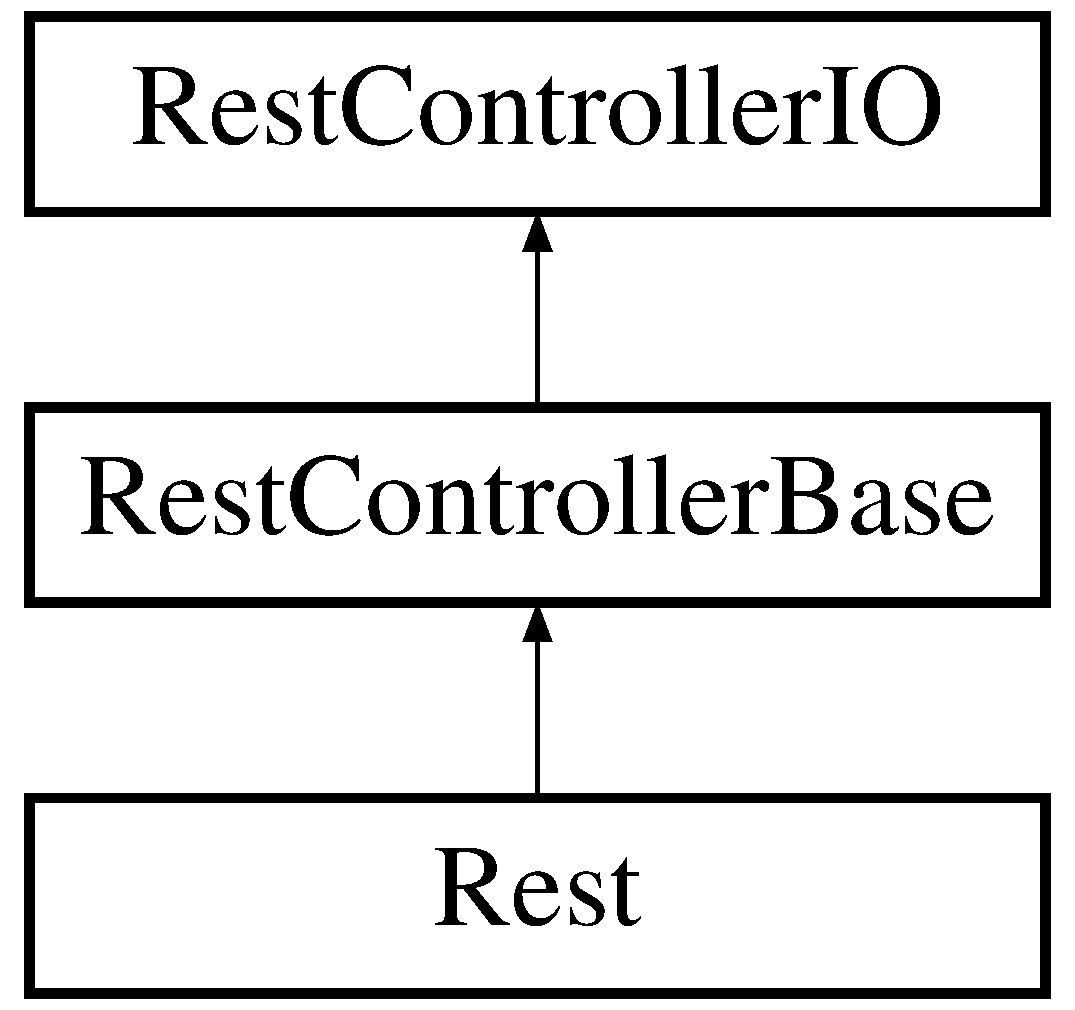
\includegraphics[height=3.000000cm]{interface_rest_controller_i_o}
\end{center}
\end{figure}
\subsection*{公開メンバ関数}
\begin{DoxyCompactItemize}
\item 
\hyperlink{interface_rest_controller_i_o_af268b91d81734f22569982048ae81a1f}{get} ()
\item 
\hyperlink{interface_rest_controller_i_o_a7794cde539999775d8401934d3087b97}{post} ()
\item 
\hyperlink{interface_rest_controller_i_o_aff718592723dba44e0dcc0c72fea183c}{put} ()
\item 
\hyperlink{interface_rest_controller_i_o_aea37c094d38f5c7ff6b5a52e9f4f30a6}{delete} ()
\end{DoxyCompactItemize}


\subsection{関数詳解}
\hypertarget{interface_rest_controller_i_o_aea37c094d38f5c7ff6b5a52e9f4f30a6}{}\index{Rest\+Controller\+I\+O@{Rest\+Controller\+I\+O}!delete@{delete}}
\index{delete@{delete}!Rest\+Controller\+I\+O@{Rest\+Controller\+I\+O}}
\subsubsection[{delete}]{\setlength{\rightskip}{0pt plus 5cm}Rest\+Controller\+I\+O\+::delete (
\begin{DoxyParamCaption}
{}
\end{DoxyParamCaption}
)}\label{interface_rest_controller_i_o_aea37c094d38f5c7ff6b5a52e9f4f30a6}
D\+E\+L\+E\+T\+Eメソッド 

\hyperlink{class_rest_controller_base_a1a30a132626984159384c227f5cdc717}{Rest\+Controller\+Base}, \hyperlink{class_rest_ad7d643a90903bc310129f8c5371ae9b3}{Rest}で実装されています。

\hypertarget{interface_rest_controller_i_o_af268b91d81734f22569982048ae81a1f}{}\index{Rest\+Controller\+I\+O@{Rest\+Controller\+I\+O}!get@{get}}
\index{get@{get}!Rest\+Controller\+I\+O@{Rest\+Controller\+I\+O}}
\subsubsection[{get}]{\setlength{\rightskip}{0pt plus 5cm}Rest\+Controller\+I\+O\+::get (
\begin{DoxyParamCaption}
{}
\end{DoxyParamCaption}
)}\label{interface_rest_controller_i_o_af268b91d81734f22569982048ae81a1f}
G\+E\+Tメソッド 

\hyperlink{class_rest_controller_base_a842a9ecef6680268e367a44c4df951a2}{Rest\+Controller\+Base}, \hyperlink{class_rest_a6b69aeaec7507e4544cf13cfe402a7cb}{Rest}で実装されています。

\hypertarget{interface_rest_controller_i_o_a7794cde539999775d8401934d3087b97}{}\index{Rest\+Controller\+I\+O@{Rest\+Controller\+I\+O}!post@{post}}
\index{post@{post}!Rest\+Controller\+I\+O@{Rest\+Controller\+I\+O}}
\subsubsection[{post}]{\setlength{\rightskip}{0pt plus 5cm}Rest\+Controller\+I\+O\+::post (
\begin{DoxyParamCaption}
{}
\end{DoxyParamCaption}
)}\label{interface_rest_controller_i_o_a7794cde539999775d8401934d3087b97}
P\+O\+S\+Tメソッド \hypertarget{interface_rest_controller_i_o_aff718592723dba44e0dcc0c72fea183c}{}\index{Rest\+Controller\+I\+O@{Rest\+Controller\+I\+O}!put@{put}}
\index{put@{put}!Rest\+Controller\+I\+O@{Rest\+Controller\+I\+O}}
\subsubsection[{put}]{\setlength{\rightskip}{0pt plus 5cm}Rest\+Controller\+I\+O\+::put (
\begin{DoxyParamCaption}
{}
\end{DoxyParamCaption}
)}\label{interface_rest_controller_i_o_aff718592723dba44e0dcc0c72fea183c}
P\+U\+Tメソッド 

このインタフェース詳解は次のファイルから抽出されました\+:\begin{DoxyCompactItemize}
\item 
Framework\+Package/class/\+M\+V\+C/Rest\+Controller\+I\+O.\+interface.\+php\end{DoxyCompactItemize}

\hypertarget{class_r_e_s_t_exception}{}\section{R\+E\+S\+T\+Exception クラス}
\label{class_r_e_s_t_exception}\index{R\+E\+S\+T\+Exception@{R\+E\+S\+T\+Exception}}
R\+E\+S\+T\+Exception の継承関係図\begin{figure}[H]
\begin{center}
\leavevmode
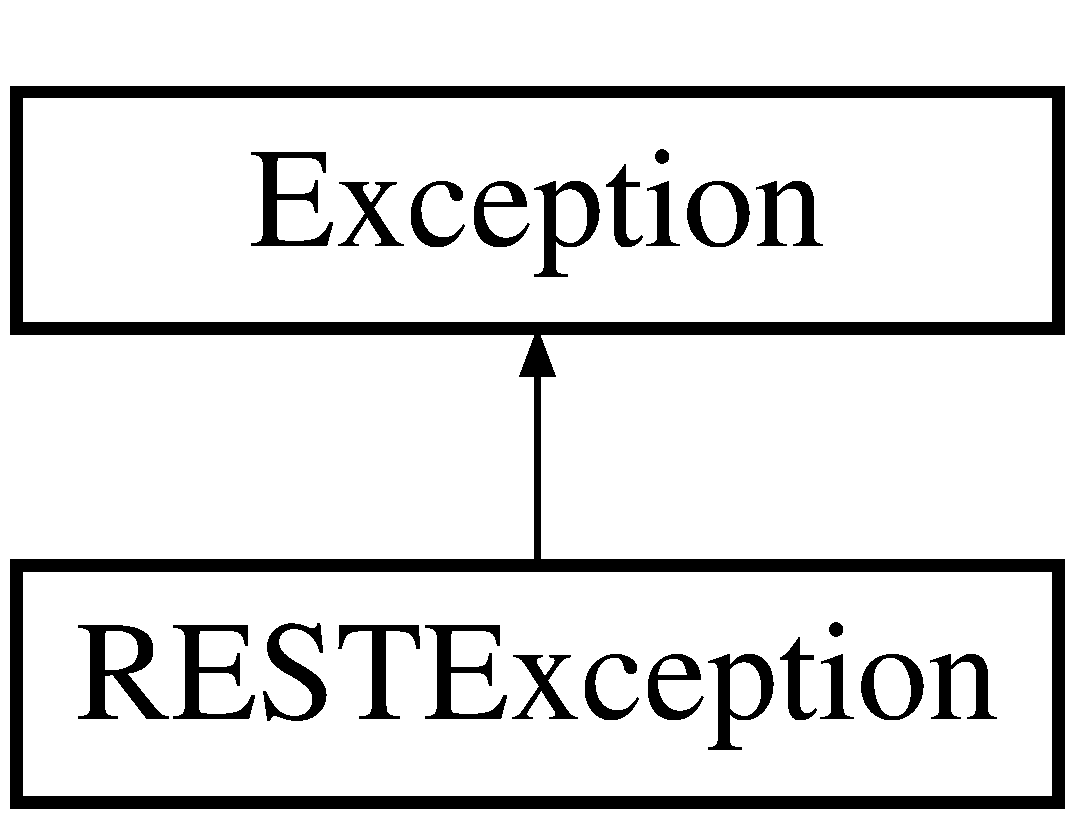
\includegraphics[height=2.000000cm]{class_r_e_s_t_exception}
\end{center}
\end{figure}
\subsection*{公開メンバ関数}
\begin{DoxyCompactItemize}
\item 
\hypertarget{class_r_e_s_t_exception_acf96f079ad04da8dba02c62d65450c98}{}{\bfseries \+\_\+\+\_\+construct} (\$arg\+Error, \$arg\+Code=N\+U\+L\+L, \$arg\+Previus=N\+U\+L\+L)\label{class_r_e_s_t_exception_acf96f079ad04da8dba02c62d65450c98}

\end{DoxyCompactItemize}


このクラス詳解は次のファイルから抽出されました\+:\begin{DoxyCompactItemize}
\item 
Framework\+Package/class/\+Exception/R\+E\+S\+T\+Exception.\+class.\+php\end{DoxyCompactItemize}

\hypertarget{class_session_data_d_b}{}\section{Session\+Data\+D\+B クラス}
\label{class_session_data_d_b}\index{Session\+Data\+D\+B@{Session\+Data\+D\+B}}
Session\+Data\+D\+B の継承関係図\begin{figure}[H]
\begin{center}
\leavevmode
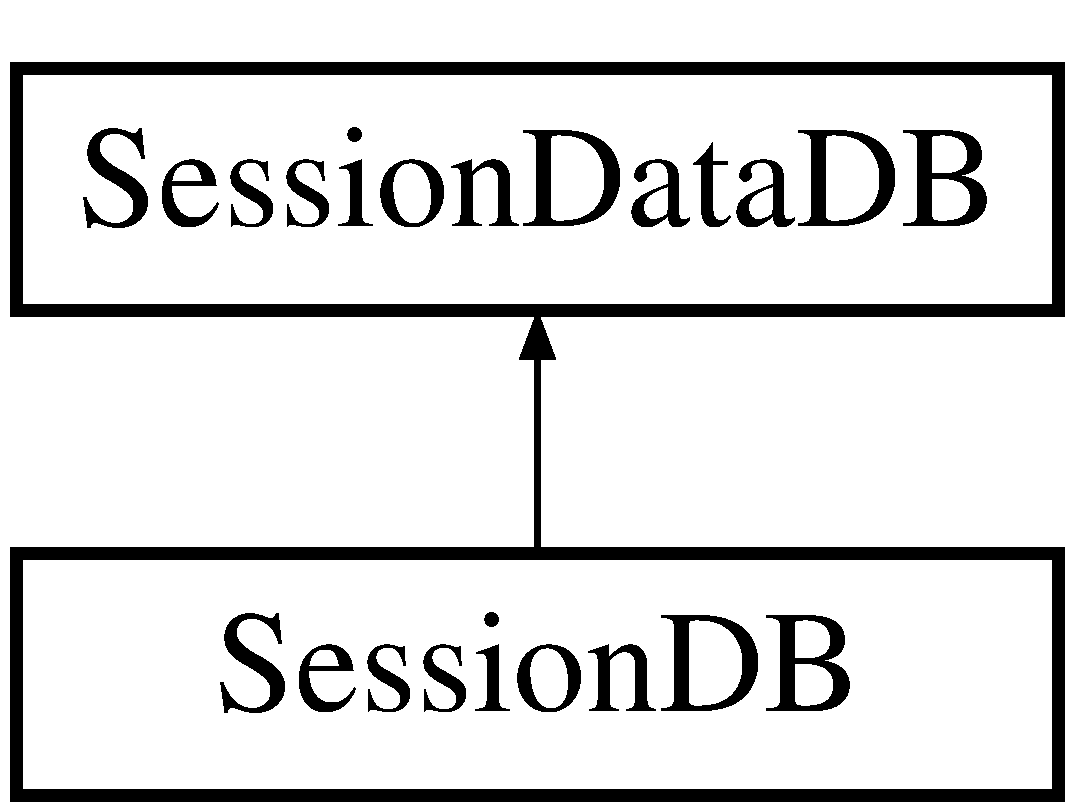
\includegraphics[height=2.000000cm]{class_session_data_d_b}
\end{center}
\end{figure}
\subsection*{静的公開メンバ関数}
\begin{DoxyCompactItemize}
\item 
static \hyperlink{class_session_data_d_b_a30a6d59940e834b23526a6db33426c12}{count} ()
\item 
static \hyperlink{class_session_data_d_b_a5ead6e650d4dc5995055fbac20e10313}{keys} ()
\item 
static \hyperlink{class_session_data_d_b_a24bd89e237f187754ee975eec333145c}{get} (\$arg\+P\+Key, \$arg\+Key=N\+U\+L\+L, \$arg\+Expiredtime=N\+U\+L\+L, \$arg\+D\+S\+N=N\+U\+L\+L)
\item 
static \hyperlink{class_session_data_d_b_a989a00d64948f48d38e7f00cce59d260}{set} (\$arg\+P\+Key, \$arg\+Key, \$argment, \$arg\+Expiredtime=N\+U\+L\+L, \$arg\+D\+S\+N=N\+U\+L\+L)
\item 
static \hyperlink{class_session_data_d_b_a35c45b3fa9727b478fdcde5909af9b79}{remove} (\$arg\+P\+Key, \$arg\+Key, \$arg\+Expiredtime=N\+U\+L\+L, \$arg\+D\+S\+N=N\+U\+L\+L)
\item 
static \hyperlink{class_session_data_d_b_aaeb3d693283e237081b09cfeeaf08d79}{clear} (\$arg\+P\+Key=N\+U\+L\+L, \$arg\+Expiredtime=N\+U\+L\+L, \$arg\+D\+S\+N=N\+U\+L\+L)
\item 
static \hyperlink{class_session_data_d_b_a36aedcb2b3168ec01821468849fae5ed}{clean} (\$arg\+Expiredtime=N\+U\+L\+L, \$arg\+D\+S\+N=N\+U\+L\+L)
\end{DoxyCompactItemize}
\subsection*{静的限定公開メンバ関数}
\begin{DoxyCompactItemize}
\item 
static \hyperlink{class_session_data_d_b_a620d706ba28277c7b81195a6eed29ef4}{\+\_\+init} (\$arg\+Expiredtime=N\+U\+L\+L, \$arg\+D\+S\+N=N\+U\+L\+L)
\item 
static \hyperlink{class_session_data_d_b_a1e5ef25b9f9a6b7931658e69facbed46}{\+\_\+initialize\+Data} (\$arg\+P\+Key)
\item 
static \hyperlink{class_session_data_d_b_a0310669f6d2bc51db4d75828fd1700c2}{\+\_\+finalize\+Data} (\$arg\+P\+Key)
\end{DoxyCompactItemize}
\subsection*{静的限定公開変数類}
\begin{DoxyCompactItemize}
\item 
\hypertarget{class_session_data_d_b_a198c6370f10af8501e23e063647a900e}{}static {\bfseries \$\+\_\+initialized} = F\+A\+L\+S\+E\label{class_session_data_d_b_a198c6370f10af8501e23e063647a900e}

\item 
\hypertarget{class_session_data_d_b_a481c0a95033cdb87358a864b12f03ec5}{}static {\bfseries \$\+\_\+expiredtime} = 3600\label{class_session_data_d_b_a481c0a95033cdb87358a864b12f03ec5}

\item 
\hypertarget{class_session_data_d_b_a63ba0b8b390947552d288104fde0f1d9}{}static {\bfseries \$\+\_\+session\+Data\+Tbl\+Name} = \textquotesingle{}session\+\_\+table\textquotesingle{}\label{class_session_data_d_b_a63ba0b8b390947552d288104fde0f1d9}

\item 
\hypertarget{class_session_data_d_b_a0d32fa71ed3feb51841a22e8807aa4da}{}static {\bfseries \$\+\_\+session\+Data\+P\+Key\+Name} = \textquotesingle{}identifier\textquotesingle{}\label{class_session_data_d_b_a0d32fa71ed3feb51841a22e8807aa4da}

\item 
\hypertarget{class_session_data_d_b_adb7138e161a094c8fca2bbd626610631}{}static {\bfseries \$\+\_\+serialize\+Key\+Name} = \textquotesingle{}data\textquotesingle{}\label{class_session_data_d_b_adb7138e161a094c8fca2bbd626610631}

\item 
\hypertarget{class_session_data_d_b_ac6c46779036540efb3c7f555ae8c1cdd}{}static {\bfseries \$\+\_\+session\+Data\+Date\+Key\+Name} = \textquotesingle{}modify\+\_\+date\textquotesingle{}\label{class_session_data_d_b_ac6c46779036540efb3c7f555ae8c1cdd}

\item 
\hypertarget{class_session_data_d_b_acf9b69ea99842849f94106bcb49b4f0e}{}static {\bfseries \$\+\_\+session\+Data} = N\+U\+L\+L\label{class_session_data_d_b_acf9b69ea99842849f94106bcb49b4f0e}

\item 
\hypertarget{class_session_data_d_b_acee92134b572b463c0d46eb38df2586e}{}static {\bfseries \$\+\_\+\+D\+B\+O} = N\+U\+L\+L\label{class_session_data_d_b_acee92134b572b463c0d46eb38df2586e}

\end{DoxyCompactItemize}


\subsection{詳解}
Sessionデータクラス(D\+B版) \begin{DoxyAuthor}{著者}
saimushi 
\end{DoxyAuthor}


\subsection{関数詳解}
\hypertarget{class_session_data_d_b_a0310669f6d2bc51db4d75828fd1700c2}{}\index{Session\+Data\+D\+B@{Session\+Data\+D\+B}!\+\_\+finalize\+Data@{\+\_\+finalize\+Data}}
\index{\+\_\+finalize\+Data@{\+\_\+finalize\+Data}!Session\+Data\+D\+B@{Session\+Data\+D\+B}}
\subsubsection[{\+\_\+finalize\+Data}]{\setlength{\rightskip}{0pt plus 5cm}static Session\+Data\+D\+B\+::\+\_\+finalize\+Data (
\begin{DoxyParamCaption}
\item[{}]{\$arg\+P\+Key}
\end{DoxyParamCaption}
)\hspace{0.3cm}{\ttfamily [static]}, {\ttfamily [protected]}}\label{class_session_data_d_b_a0310669f6d2bc51db4d75828fd1700c2}
セッションデータテーブルにデータをしまう 
\begin{DoxyParams}{引数}
{\em string} & セッションデータのプライマリーキー \\
\hline
\end{DoxyParams}
\hypertarget{class_session_data_d_b_a620d706ba28277c7b81195a6eed29ef4}{}\index{Session\+Data\+D\+B@{Session\+Data\+D\+B}!\+\_\+init@{\+\_\+init}}
\index{\+\_\+init@{\+\_\+init}!Session\+Data\+D\+B@{Session\+Data\+D\+B}}
\subsubsection[{\+\_\+init}]{\setlength{\rightskip}{0pt plus 5cm}static Session\+Data\+D\+B\+::\+\_\+init (
\begin{DoxyParamCaption}
\item[{}]{\$arg\+Expiredtime = {\ttfamily NULL}, }
\item[{}]{\$arg\+D\+S\+N = {\ttfamily NULL}}
\end{DoxyParamCaption}
)\hspace{0.3cm}{\ttfamily [static]}, {\ttfamily [protected]}}\label{class_session_data_d_b_a620d706ba28277c7b81195a6eed29ef4}
Sessionクラスの初期化 
\begin{DoxyParams}{引数}
{\em string} & セッションの有効期限 \\
\hline
{\em string} & D\+B\+D\+S\+N情報 \\
\hline
\end{DoxyParams}
\hypertarget{class_session_data_d_b_a1e5ef25b9f9a6b7931658e69facbed46}{}\index{Session\+Data\+D\+B@{Session\+Data\+D\+B}!\+\_\+initialize\+Data@{\+\_\+initialize\+Data}}
\index{\+\_\+initialize\+Data@{\+\_\+initialize\+Data}!Session\+Data\+D\+B@{Session\+Data\+D\+B}}
\subsubsection[{\+\_\+initialize\+Data}]{\setlength{\rightskip}{0pt plus 5cm}static Session\+Data\+D\+B\+::\+\_\+initialize\+Data (
\begin{DoxyParamCaption}
\item[{}]{\$arg\+P\+Key}
\end{DoxyParamCaption}
)\hspace{0.3cm}{\ttfamily [static]}, {\ttfamily [protected]}}\label{class_session_data_d_b_a1e5ef25b9f9a6b7931658e69facbed46}
セッションデータデーブルからデータを取得し復元する 
\begin{DoxyParams}{引数}
{\em string} & セッションデータのプライマリーキー \\
\hline
\end{DoxyParams}
\hypertarget{class_session_data_d_b_a36aedcb2b3168ec01821468849fae5ed}{}\index{Session\+Data\+D\+B@{Session\+Data\+D\+B}!clean@{clean}}
\index{clean@{clean}!Session\+Data\+D\+B@{Session\+Data\+D\+B}}
\subsubsection[{clean}]{\setlength{\rightskip}{0pt plus 5cm}static Session\+Data\+D\+B\+::clean (
\begin{DoxyParamCaption}
\item[{}]{\$arg\+Expiredtime = {\ttfamily NULL}, }
\item[{}]{\$arg\+D\+S\+N = {\ttfamily NULL}}
\end{DoxyParamCaption}
)\hspace{0.3cm}{\ttfamily [static]}}\label{class_session_data_d_b_a36aedcb2b3168ec01821468849fae5ed}
Expiredの切れた\+Sessionレコードを\+Deleteする 
\begin{DoxyParams}{引数}
{\em int} & 有効期限の直指定 \\
\hline
{\em mixed} & D\+B\+D\+S\+N情報の直指定 \\
\hline
\end{DoxyParams}
\hypertarget{class_session_data_d_b_aaeb3d693283e237081b09cfeeaf08d79}{}\index{Session\+Data\+D\+B@{Session\+Data\+D\+B}!clear@{clear}}
\index{clear@{clear}!Session\+Data\+D\+B@{Session\+Data\+D\+B}}
\subsubsection[{clear}]{\setlength{\rightskip}{0pt plus 5cm}static Session\+Data\+D\+B\+::clear (
\begin{DoxyParamCaption}
\item[{}]{\$arg\+P\+Key = {\ttfamily NULL}, }
\item[{}]{\$arg\+Expiredtime = {\ttfamily NULL}, }
\item[{}]{\$arg\+D\+S\+N = {\ttfamily NULL}}
\end{DoxyParamCaption}
)\hspace{0.3cm}{\ttfamily [static]}}\label{class_session_data_d_b_aaeb3d693283e237081b09cfeeaf08d79}
identifierに紐づくセッションデータレコードをクリアする 
\begin{DoxyParams}{引数}
{\em string} & セッションデータのプライマリーキー \\
\hline
{\em int} & 有効期限の直指定 \\
\hline
{\em mixed} & D\+B\+D\+S\+N情報の直指定 \\
\hline
\end{DoxyParams}
\hypertarget{class_session_data_d_b_a30a6d59940e834b23526a6db33426c12}{}\index{Session\+Data\+D\+B@{Session\+Data\+D\+B}!count@{count}}
\index{count@{count}!Session\+Data\+D\+B@{Session\+Data\+D\+B}}
\subsubsection[{count}]{\setlength{\rightskip}{0pt plus 5cm}static Session\+Data\+D\+B\+::count (
\begin{DoxyParamCaption}
{}
\end{DoxyParamCaption}
)\hspace{0.3cm}{\ttfamily [static]}}\label{class_session_data_d_b_a30a6d59940e834b23526a6db33426c12}
セッションデータのキーの数を返す \hypertarget{class_session_data_d_b_a24bd89e237f187754ee975eec333145c}{}\index{Session\+Data\+D\+B@{Session\+Data\+D\+B}!get@{get}}
\index{get@{get}!Session\+Data\+D\+B@{Session\+Data\+D\+B}}
\subsubsection[{get}]{\setlength{\rightskip}{0pt plus 5cm}static Session\+Data\+D\+B\+::get (
\begin{DoxyParamCaption}
\item[{}]{\$arg\+P\+Key, }
\item[{}]{\$arg\+Key = {\ttfamily NULL}, }
\item[{}]{\$arg\+Expiredtime = {\ttfamily NULL}, }
\item[{}]{\$arg\+D\+S\+N = {\ttfamily NULL}}
\end{DoxyParamCaption}
)\hspace{0.3cm}{\ttfamily [static]}}\label{class_session_data_d_b_a24bd89e237f187754ee975eec333145c}
セッションデータの指定のキー名で保存されたデータを返す 
\begin{DoxyParams}{引数}
{\em string} & セッションデータのプライマリーキー \\
\hline
{\em string} & キー名 \\
\hline
{\em mixed} & 変数全て(P\+H\+Pオブジェクトは保存出来ない!) \\
\hline
{\em int} & 有効期限の直指定 \\
\hline
{\em mixed} & D\+B\+D\+S\+N情報の直指定 \\
\hline
\end{DoxyParams}
\hypertarget{class_session_data_d_b_a5ead6e650d4dc5995055fbac20e10313}{}\index{Session\+Data\+D\+B@{Session\+Data\+D\+B}!keys@{keys}}
\index{keys@{keys}!Session\+Data\+D\+B@{Session\+Data\+D\+B}}
\subsubsection[{keys}]{\setlength{\rightskip}{0pt plus 5cm}static Session\+Data\+D\+B\+::keys (
\begin{DoxyParamCaption}
{}
\end{DoxyParamCaption}
)\hspace{0.3cm}{\ttfamily [static]}}\label{class_session_data_d_b_a5ead6e650d4dc5995055fbac20e10313}
セッションデータのキーの一覧を返す \hypertarget{class_session_data_d_b_a35c45b3fa9727b478fdcde5909af9b79}{}\index{Session\+Data\+D\+B@{Session\+Data\+D\+B}!remove@{remove}}
\index{remove@{remove}!Session\+Data\+D\+B@{Session\+Data\+D\+B}}
\subsubsection[{remove}]{\setlength{\rightskip}{0pt plus 5cm}static Session\+Data\+D\+B\+::remove (
\begin{DoxyParamCaption}
\item[{}]{\$arg\+P\+Key, }
\item[{}]{\$arg\+Key, }
\item[{}]{\$arg\+Expiredtime = {\ttfamily NULL}, }
\item[{}]{\$arg\+D\+S\+N = {\ttfamily NULL}}
\end{DoxyParamCaption}
)\hspace{0.3cm}{\ttfamily [static]}}\label{class_session_data_d_b_a35c45b3fa9727b478fdcde5909af9b79}
セッションデータに指定のキー名の値を削除する 
\begin{DoxyParams}{引数}
{\em string} & セッションデータのプライマリーキー \\
\hline
{\em string} & キー名 \\
\hline
{\em mixed} & 変数全て(P\+H\+Pオブジェクトは保存出来ない!) \\
\hline
{\em int} & 有効期限の直指定 \\
\hline
{\em mixed} & D\+B\+D\+S\+N情報の直指定 \\
\hline
\end{DoxyParams}
\hypertarget{class_session_data_d_b_a989a00d64948f48d38e7f00cce59d260}{}\index{Session\+Data\+D\+B@{Session\+Data\+D\+B}!set@{set}}
\index{set@{set}!Session\+Data\+D\+B@{Session\+Data\+D\+B}}
\subsubsection[{set}]{\setlength{\rightskip}{0pt plus 5cm}static Session\+Data\+D\+B\+::set (
\begin{DoxyParamCaption}
\item[{}]{\$arg\+P\+Key, }
\item[{}]{\$arg\+Key, }
\item[{}]{\$argment, }
\item[{}]{\$arg\+Expiredtime = {\ttfamily NULL}, }
\item[{}]{\$arg\+D\+S\+N = {\ttfamily NULL}}
\end{DoxyParamCaption}
)\hspace{0.3cm}{\ttfamily [static]}}\label{class_session_data_d_b_a989a00d64948f48d38e7f00cce59d260}
セッションデータに指定のキー名で指定のデータを追加する 
\begin{DoxyParams}{引数}
{\em string} & セッションデータのプライマリーキー \\
\hline
{\em string} & キー名 \\
\hline
{\em mixed} & 変数全て(P\+H\+Pオブジェクトは保存出来ない!) \\
\hline
{\em int} & 有効期限の直指定 \\
\hline
{\em mixed} & D\+B\+D\+S\+N情報の直指定 \\
\hline
\end{DoxyParams}


このクラス詳解は次のファイルから抽出されました\+:\begin{DoxyCompactItemize}
\item 
Framework\+Package/class/\+Session/Session\+Data\+D\+B.\+abstract.\+php\end{DoxyCompactItemize}

\hypertarget{class_session_data_memcache}{}\section{Session\+Data\+Memcache クラス}
\label{class_session_data_memcache}\index{Session\+Data\+Memcache@{Session\+Data\+Memcache}}
Session\+Data\+Memcache の継承関係図\begin{figure}[H]
\begin{center}
\leavevmode
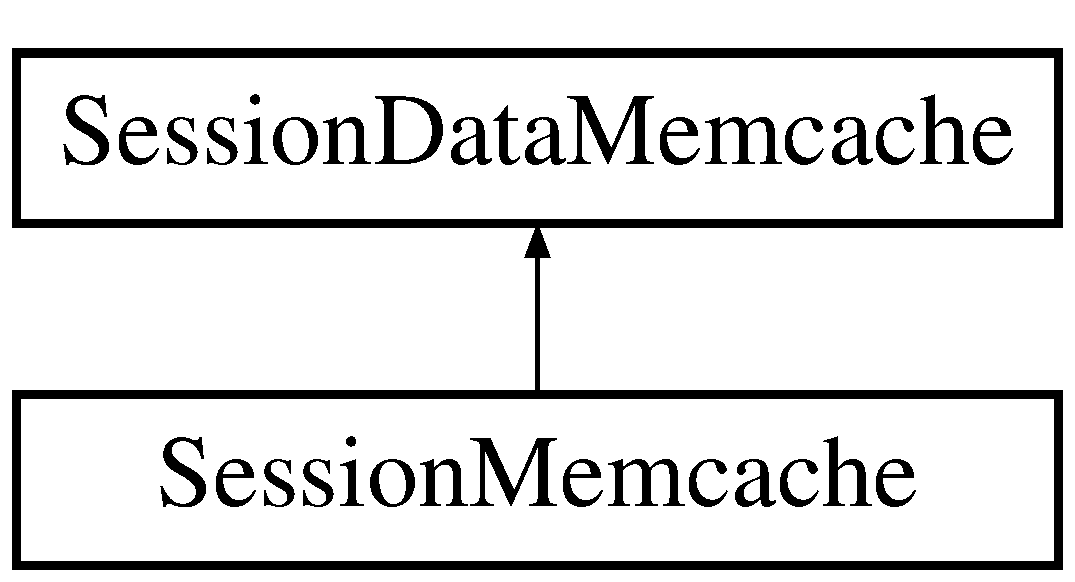
\includegraphics[height=2.000000cm]{class_session_data_memcache}
\end{center}
\end{figure}
\subsection*{静的公開メンバ関数}
\begin{DoxyCompactItemize}
\item 
static \hyperlink{class_session_data_memcache_a41ee61ffc192ecca6986be329897752f}{count} ()
\item 
static \hyperlink{class_session_data_memcache_af0d822a1b1cfa15344c03c762df345d2}{keys} ()
\item 
static \hyperlink{class_session_data_memcache_a2fcf53acfd7032e09e2a8465165c47e6}{get} (\$arg\+P\+Key, \$arg\+Key=N\+U\+L\+L, \$arg\+Expiredtime=N\+U\+L\+L, \$arg\+D\+S\+N=N\+U\+L\+L)
\item 
static \hyperlink{class_session_data_memcache_a7735cb0fc5b6c136ae76b19aba68173a}{set} (\$arg\+P\+Key, \$arg\+Key, \$argment, \$arg\+Expiredtime=N\+U\+L\+L, \$arg\+D\+S\+N=N\+U\+L\+L)
\item 
static \hyperlink{class_session_data_memcache_aa399bbfbd3f4706e952317f76aadfe01}{remove} (\$arg\+P\+Key, \$arg\+Key, \$arg\+Expiredtime=N\+U\+L\+L, \$arg\+D\+S\+N=N\+U\+L\+L)
\item 
static \hyperlink{class_session_data_memcache_af06195254f5eec93998c4eb2569bc140}{clear} (\$arg\+P\+Key=N\+U\+L\+L, \$arg\+Expiredtime=N\+U\+L\+L, \$arg\+D\+S\+N=N\+U\+L\+L)
\item 
static \hyperlink{class_session_data_memcache_af09867c8e3d262ee7c0aad65be21f7f4}{clean} (\$arg\+Expiredtime=N\+U\+L\+L, \$arg\+D\+S\+N=N\+U\+L\+L)
\end{DoxyCompactItemize}
\subsection*{静的限定公開メンバ関数}
\begin{DoxyCompactItemize}
\item 
static \hyperlink{class_session_data_memcache_a1022edb4a06d9ccdad6defe968138284}{\+\_\+init} (\$arg\+Expiredtime=N\+U\+L\+L, \$arg\+D\+S\+N=N\+U\+L\+L)
\item 
static \hyperlink{class_session_data_memcache_a453fa5b1a8e999377b726dc7bce92ee6}{\+\_\+initialize\+Data} (\$arg\+P\+Key)
\item 
static \hyperlink{class_session_data_memcache_a39978a1adfb67fe1add5053cabfce074}{\+\_\+finalize\+Data} (\$arg\+P\+Key)
\end{DoxyCompactItemize}
\subsection*{静的限定公開変数類}
\begin{DoxyCompactItemize}
\item 
\hypertarget{class_session_data_memcache_a2e3e68055a5bb996b545c07cc7a3fa68}{}static {\bfseries \$\+\_\+initialized} = F\+A\+L\+S\+E\label{class_session_data_memcache_a2e3e68055a5bb996b545c07cc7a3fa68}

\item 
\hypertarget{class_session_data_memcache_abddda812f41089fbfb5f9d53414ffe8f}{}static {\bfseries \$\+\_\+expiredtime} = 3600\label{class_session_data_memcache_abddda812f41089fbfb5f9d53414ffe8f}

\item 
\hypertarget{class_session_data_memcache_a7b0cd680ea173915e29e35c4680b4235}{}static {\bfseries \$\+\_\+session\+Data\+Tbl\+Name} = \textquotesingle{}session\+\_\+table\textquotesingle{}\label{class_session_data_memcache_a7b0cd680ea173915e29e35c4680b4235}

\item 
\hypertarget{class_session_data_memcache_a2da0ed1e581f4765b21972d32e58bbe8}{}static {\bfseries \$\+\_\+session\+Data\+P\+Key\+Name} = \textquotesingle{}identifier\textquotesingle{}\label{class_session_data_memcache_a2da0ed1e581f4765b21972d32e58bbe8}

\item 
\hypertarget{class_session_data_memcache_a35d1534fc9568511f88982be2d88ea82}{}static {\bfseries \$\+\_\+serialize\+Key\+Name} = \textquotesingle{}data\textquotesingle{}\label{class_session_data_memcache_a35d1534fc9568511f88982be2d88ea82}

\item 
\hypertarget{class_session_data_memcache_a73f8598f2c048580eb60d44acc7218ba}{}static {\bfseries \$\+\_\+session\+Data\+Date\+Key\+Name} = \textquotesingle{}modify\+\_\+date\textquotesingle{}\label{class_session_data_memcache_a73f8598f2c048580eb60d44acc7218ba}

\item 
\hypertarget{class_session_data_memcache_a79e29d0127e55d3b140bf0aa70ea78a9}{}static {\bfseries \$\+\_\+session\+Data} = N\+U\+L\+L\label{class_session_data_memcache_a79e29d0127e55d3b140bf0aa70ea78a9}

\item 
\hypertarget{class_session_data_memcache_a51d7024dcc926acfaaab0d818b7e1750}{}static {\bfseries \$\+\_\+\+D\+S\+N} = N\+U\+L\+L\label{class_session_data_memcache_a51d7024dcc926acfaaab0d818b7e1750}

\end{DoxyCompactItemize}


\subsection{詳解}
Sessionデータクラス(P\+E\+C\+L\+:Memcache版(非\+P\+E\+C\+L\+:Memcached)) \begin{DoxyAuthor}{著者}
saimushi 
\end{DoxyAuthor}


\subsection{関数詳解}
\hypertarget{class_session_data_memcache_a39978a1adfb67fe1add5053cabfce074}{}\index{Session\+Data\+Memcache@{Session\+Data\+Memcache}!\+\_\+finalize\+Data@{\+\_\+finalize\+Data}}
\index{\+\_\+finalize\+Data@{\+\_\+finalize\+Data}!Session\+Data\+Memcache@{Session\+Data\+Memcache}}
\subsubsection[{\+\_\+finalize\+Data}]{\setlength{\rightskip}{0pt plus 5cm}static Session\+Data\+Memcache\+::\+\_\+finalize\+Data (
\begin{DoxyParamCaption}
\item[{}]{\$arg\+P\+Key}
\end{DoxyParamCaption}
)\hspace{0.3cm}{\ttfamily [static]}, {\ttfamily [protected]}}\label{class_session_data_memcache_a39978a1adfb67fe1add5053cabfce074}
セッションデータテーブルにデータをしまう 
\begin{DoxyParams}{引数}
{\em string} & セッションデータのプライマリーキー \\
\hline
\end{DoxyParams}
\hypertarget{class_session_data_memcache_a1022edb4a06d9ccdad6defe968138284}{}\index{Session\+Data\+Memcache@{Session\+Data\+Memcache}!\+\_\+init@{\+\_\+init}}
\index{\+\_\+init@{\+\_\+init}!Session\+Data\+Memcache@{Session\+Data\+Memcache}}
\subsubsection[{\+\_\+init}]{\setlength{\rightskip}{0pt plus 5cm}static Session\+Data\+Memcache\+::\+\_\+init (
\begin{DoxyParamCaption}
\item[{}]{\$arg\+Expiredtime = {\ttfamily NULL}, }
\item[{}]{\$arg\+D\+S\+N = {\ttfamily NULL}}
\end{DoxyParamCaption}
)\hspace{0.3cm}{\ttfamily [static]}, {\ttfamily [protected]}}\label{class_session_data_memcache_a1022edb4a06d9ccdad6defe968138284}
Sessionクラスの初期化 
\begin{DoxyParams}{引数}
{\em string} & セッションの有効期限 \\
\hline
{\em string} & D\+B\+D\+S\+N情報 \\
\hline
\end{DoxyParams}
\hypertarget{class_session_data_memcache_a453fa5b1a8e999377b726dc7bce92ee6}{}\index{Session\+Data\+Memcache@{Session\+Data\+Memcache}!\+\_\+initialize\+Data@{\+\_\+initialize\+Data}}
\index{\+\_\+initialize\+Data@{\+\_\+initialize\+Data}!Session\+Data\+Memcache@{Session\+Data\+Memcache}}
\subsubsection[{\+\_\+initialize\+Data}]{\setlength{\rightskip}{0pt plus 5cm}static Session\+Data\+Memcache\+::\+\_\+initialize\+Data (
\begin{DoxyParamCaption}
\item[{}]{\$arg\+P\+Key}
\end{DoxyParamCaption}
)\hspace{0.3cm}{\ttfamily [static]}, {\ttfamily [protected]}}\label{class_session_data_memcache_a453fa5b1a8e999377b726dc7bce92ee6}
セッションデータデーブルからデータを取得し復元する 
\begin{DoxyParams}{引数}
{\em string} & セッションデータのプライマリーキー \\
\hline
\end{DoxyParams}
\hypertarget{class_session_data_memcache_af09867c8e3d262ee7c0aad65be21f7f4}{}\index{Session\+Data\+Memcache@{Session\+Data\+Memcache}!clean@{clean}}
\index{clean@{clean}!Session\+Data\+Memcache@{Session\+Data\+Memcache}}
\subsubsection[{clean}]{\setlength{\rightskip}{0pt plus 5cm}static Session\+Data\+Memcache\+::clean (
\begin{DoxyParamCaption}
\item[{}]{\$arg\+Expiredtime = {\ttfamily NULL}, }
\item[{}]{\$arg\+D\+S\+N = {\ttfamily NULL}}
\end{DoxyParamCaption}
)\hspace{0.3cm}{\ttfamily [static]}}\label{class_session_data_memcache_af09867c8e3d262ee7c0aad65be21f7f4}
Expiredの切れた\+Sessionレコードを\+Deleteする 
\begin{DoxyParams}{引数}
{\em int} & 有効期限の直指定 \\
\hline
{\em mixed} & D\+B\+D\+S\+N情報の直指定 \\
\hline
\end{DoxyParams}
\hypertarget{class_session_data_memcache_af06195254f5eec93998c4eb2569bc140}{}\index{Session\+Data\+Memcache@{Session\+Data\+Memcache}!clear@{clear}}
\index{clear@{clear}!Session\+Data\+Memcache@{Session\+Data\+Memcache}}
\subsubsection[{clear}]{\setlength{\rightskip}{0pt plus 5cm}static Session\+Data\+Memcache\+::clear (
\begin{DoxyParamCaption}
\item[{}]{\$arg\+P\+Key = {\ttfamily NULL}, }
\item[{}]{\$arg\+Expiredtime = {\ttfamily NULL}, }
\item[{}]{\$arg\+D\+S\+N = {\ttfamily NULL}}
\end{DoxyParamCaption}
)\hspace{0.3cm}{\ttfamily [static]}}\label{class_session_data_memcache_af06195254f5eec93998c4eb2569bc140}
identifierに紐づくセッションデータレコードをクリアする 
\begin{DoxyParams}{引数}
{\em string} & セッションデータのプライマリーキー \\
\hline
{\em int} & 有効期限の直指定 \\
\hline
{\em mixed} & D\+B\+D\+S\+N情報の直指定 \\
\hline
\end{DoxyParams}
\hypertarget{class_session_data_memcache_a41ee61ffc192ecca6986be329897752f}{}\index{Session\+Data\+Memcache@{Session\+Data\+Memcache}!count@{count}}
\index{count@{count}!Session\+Data\+Memcache@{Session\+Data\+Memcache}}
\subsubsection[{count}]{\setlength{\rightskip}{0pt plus 5cm}static Session\+Data\+Memcache\+::count (
\begin{DoxyParamCaption}
{}
\end{DoxyParamCaption}
)\hspace{0.3cm}{\ttfamily [static]}}\label{class_session_data_memcache_a41ee61ffc192ecca6986be329897752f}
セッションデータのキーの数を返す \hypertarget{class_session_data_memcache_a2fcf53acfd7032e09e2a8465165c47e6}{}\index{Session\+Data\+Memcache@{Session\+Data\+Memcache}!get@{get}}
\index{get@{get}!Session\+Data\+Memcache@{Session\+Data\+Memcache}}
\subsubsection[{get}]{\setlength{\rightskip}{0pt plus 5cm}static Session\+Data\+Memcache\+::get (
\begin{DoxyParamCaption}
\item[{}]{\$arg\+P\+Key, }
\item[{}]{\$arg\+Key = {\ttfamily NULL}, }
\item[{}]{\$arg\+Expiredtime = {\ttfamily NULL}, }
\item[{}]{\$arg\+D\+S\+N = {\ttfamily NULL}}
\end{DoxyParamCaption}
)\hspace{0.3cm}{\ttfamily [static]}}\label{class_session_data_memcache_a2fcf53acfd7032e09e2a8465165c47e6}
セッションデータの指定のキー名で保存されたデータを返す 
\begin{DoxyParams}{引数}
{\em string} & セッションデータのプライマリーキー \\
\hline
{\em string} & キー名 \\
\hline
{\em mixed} & 変数全て(P\+H\+Pオブジェクトは保存出来ない!) \\
\hline
{\em int} & 有効期限の直指定 \\
\hline
{\em mixed} & D\+B\+D\+S\+N情報の直指定 \\
\hline
\end{DoxyParams}
\hypertarget{class_session_data_memcache_af0d822a1b1cfa15344c03c762df345d2}{}\index{Session\+Data\+Memcache@{Session\+Data\+Memcache}!keys@{keys}}
\index{keys@{keys}!Session\+Data\+Memcache@{Session\+Data\+Memcache}}
\subsubsection[{keys}]{\setlength{\rightskip}{0pt plus 5cm}static Session\+Data\+Memcache\+::keys (
\begin{DoxyParamCaption}
{}
\end{DoxyParamCaption}
)\hspace{0.3cm}{\ttfamily [static]}}\label{class_session_data_memcache_af0d822a1b1cfa15344c03c762df345d2}
セッションデータのキーの一覧を返す \hypertarget{class_session_data_memcache_aa399bbfbd3f4706e952317f76aadfe01}{}\index{Session\+Data\+Memcache@{Session\+Data\+Memcache}!remove@{remove}}
\index{remove@{remove}!Session\+Data\+Memcache@{Session\+Data\+Memcache}}
\subsubsection[{remove}]{\setlength{\rightskip}{0pt plus 5cm}static Session\+Data\+Memcache\+::remove (
\begin{DoxyParamCaption}
\item[{}]{\$arg\+P\+Key, }
\item[{}]{\$arg\+Key, }
\item[{}]{\$arg\+Expiredtime = {\ttfamily NULL}, }
\item[{}]{\$arg\+D\+S\+N = {\ttfamily NULL}}
\end{DoxyParamCaption}
)\hspace{0.3cm}{\ttfamily [static]}}\label{class_session_data_memcache_aa399bbfbd3f4706e952317f76aadfe01}
セッションデータに指定のキー名の値を削除する 
\begin{DoxyParams}{引数}
{\em string} & セッションデータのプライマリーキー \\
\hline
{\em string} & キー名 \\
\hline
{\em mixed} & 変数全て(P\+H\+Pオブジェクトは保存出来ない!) \\
\hline
{\em int} & 有効期限の直指定 \\
\hline
{\em mixed} & D\+B\+D\+S\+N情報の直指定 \\
\hline
\end{DoxyParams}
\hypertarget{class_session_data_memcache_a7735cb0fc5b6c136ae76b19aba68173a}{}\index{Session\+Data\+Memcache@{Session\+Data\+Memcache}!set@{set}}
\index{set@{set}!Session\+Data\+Memcache@{Session\+Data\+Memcache}}
\subsubsection[{set}]{\setlength{\rightskip}{0pt plus 5cm}static Session\+Data\+Memcache\+::set (
\begin{DoxyParamCaption}
\item[{}]{\$arg\+P\+Key, }
\item[{}]{\$arg\+Key, }
\item[{}]{\$argment, }
\item[{}]{\$arg\+Expiredtime = {\ttfamily NULL}, }
\item[{}]{\$arg\+D\+S\+N = {\ttfamily NULL}}
\end{DoxyParamCaption}
)\hspace{0.3cm}{\ttfamily [static]}}\label{class_session_data_memcache_a7735cb0fc5b6c136ae76b19aba68173a}
セッションデータに指定のキー名で指定のデータを追加する 
\begin{DoxyParams}{引数}
{\em string} & セッションデータのプライマリーキー \\
\hline
{\em string} & キー名 \\
\hline
{\em mixed} & 変数全て(P\+H\+Pオブジェクトは保存出来ない!) \\
\hline
{\em int} & 有効期限の直指定 \\
\hline
{\em mixed} & D\+B\+D\+S\+N情報の直指定 \\
\hline
\end{DoxyParams}


このクラス詳解は次のファイルから抽出されました\+:\begin{DoxyCompactItemize}
\item 
Framework\+Package/class/\+Session/Session\+Data\+Memcache.\+abstract.\+php\end{DoxyCompactItemize}

\hypertarget{class_session_d_b}{}\section{Session\+D\+B クラス}
\label{class_session_d_b}\index{Session\+D\+B@{Session\+D\+B}}
Session\+D\+B の継承関係図\begin{figure}[H]
\begin{center}
\leavevmode
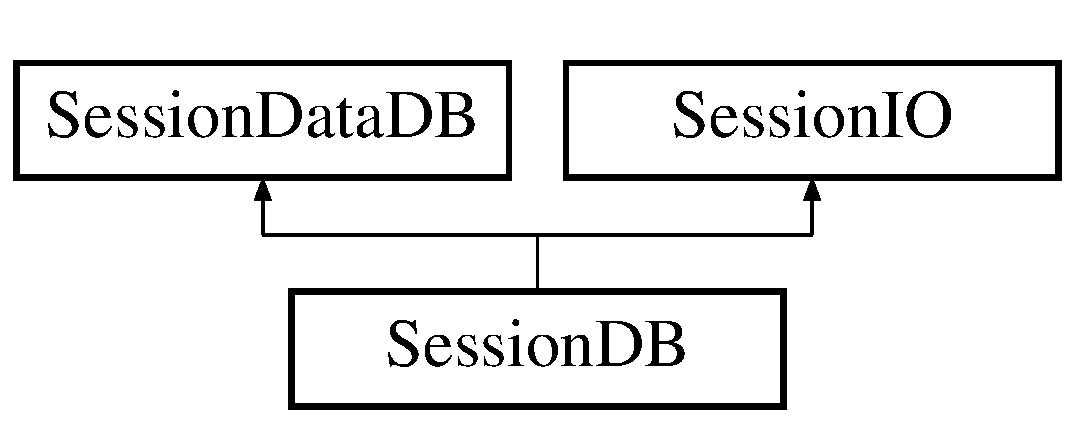
\includegraphics[height=2.000000cm]{class_session_d_b}
\end{center}
\end{figure}
\subsection*{静的公開メンバ関数}
\begin{DoxyCompactItemize}
\item 
static \hyperlink{class_session_d_b_a1229c629f73d4b80e2b3feab4147eefb}{set\+Token\+Key} (\$arg\+Token\+Key)
\item 
static \hyperlink{class_session_d_b_af7d47daa6b652fe112e59530e60df922}{set\+Token\+To\+Cookie} (\$arg\+Token\+Key)
\item 
static \hyperlink{class_session_d_b_abcf6313d78bbf6ecf53ba5fba312d55f}{session\+I\+D} (\$arg\+Identifier=N\+U\+L\+L)
\item 
static \hyperlink{class_session_d_b_a8f5f5c56a8e2307f61ac7fbc6869a272}{start} (\$arg\+Domain=N\+U\+L\+L, \$arg\+Expiredtime=N\+U\+L\+L, \$arg\+D\+S\+N=N\+U\+L\+L)
\item 
static \hyperlink{class_session_d_b_a956124a9e132a41c428e4befd24d1b52}{get} (\$arg\+Key=N\+U\+L\+L)
\item 
static \hyperlink{class_session_d_b_a14c8618d095cd1d5ba655fc673eb2488}{set} (\$arg\+Key, \$argment)
\item 
\hypertarget{class_session_d_b_a2dd2181533bf5da156da2793f11390f8}{}static {\bfseries clear} ()\label{class_session_d_b_a2dd2181533bf5da156da2793f11390f8}

\end{DoxyCompactItemize}
\subsection*{静的限定公開メンバ関数}
\begin{DoxyCompactItemize}
\item 
static \hyperlink{class_session_d_b_ad06b74e267ec7f1e1e64a09cf1ce430e}{\+\_\+init} (\$arg\+Domain=N\+U\+L\+L, \$arg\+Expiredtime=N\+U\+L\+L, \$arg\+D\+S\+N=N\+U\+L\+L)
\item 
static \hyperlink{class_session_d_b_afc4ea0089bf659a952a500d8a0106d82}{\+\_\+token\+To\+Identifier} (\$arg\+Token, \$arg\+Uncheck=F\+A\+L\+S\+E)
\item 
static \hyperlink{class_session_d_b_ad31baeaf0488fd9f7d7cecb6ac10bfcc}{\+\_\+identifier\+To\+Token} (\$arg\+Identifier)
\item 
static \hyperlink{class_session_d_b_a08b430e3942c1275034ebcc8f74478b2}{\+\_\+initialize\+Token} ()
\end{DoxyCompactItemize}
\subsection*{静的限定公開変数類}
\begin{DoxyCompactItemize}
\item 
\hypertarget{class_session_d_b_a77bb91a3e040db8421600f00d5c52b67}{}static {\bfseries \$\+\_\+\+D\+B\+O} = N\+U\+L\+L\label{class_session_d_b_a77bb91a3e040db8421600f00d5c52b67}

\item 
\hypertarget{class_session_d_b_a0e2ea2fef693d8ce80b9ffaf28865cf3}{}static {\bfseries \$\+\_\+initialized} = F\+A\+L\+S\+E\label{class_session_d_b_a0e2ea2fef693d8ce80b9ffaf28865cf3}

\item 
\hypertarget{class_session_d_b_ae2bf7a0043c7473125f676f8165bb2f1}{}static {\bfseries \$\+\_\+token\+Initialized} = F\+A\+L\+S\+E\label{class_session_d_b_ae2bf7a0043c7473125f676f8165bb2f1}

\item 
\hypertarget{class_session_d_b_a4a86fda0a7eae21f83ee0cd13bd74208}{}static {\bfseries \$\+\_\+replaced} = F\+A\+L\+S\+E\label{class_session_d_b_a4a86fda0a7eae21f83ee0cd13bd74208}

\item 
\hypertarget{class_session_d_b_afd4032dbb1bdd29753245344750b4576}{}static {\bfseries \$\+\_\+token\+Key\+Name} = \textquotesingle{}token\textquotesingle{}\label{class_session_d_b_afd4032dbb1bdd29753245344750b4576}

\item 
\hypertarget{class_session_d_b_a199d1a99b891b74e9fc7913182d9aa2b}{}static {\bfseries \$\+\_\+token} = N\+U\+L\+L\label{class_session_d_b_a199d1a99b891b74e9fc7913182d9aa2b}

\item 
\hypertarget{class_session_d_b_a919d2613a316a1bae7e843803d9eecf4}{}static {\bfseries \$\+\_\+identifier} = N\+U\+L\+L\label{class_session_d_b_a919d2613a316a1bae7e843803d9eecf4}

\item 
\hypertarget{class_session_d_b_a62dad33fe1ce06c86c1c69e9d90bd40b}{}static {\bfseries \$\+\_\+domain} = N\+U\+L\+L\label{class_session_d_b_a62dad33fe1ce06c86c1c69e9d90bd40b}

\item 
\hypertarget{class_session_d_b_a0e1d5c789bd61b7b4ef031e6b7b08ab6}{}static {\bfseries \$\+\_\+path} = \textquotesingle{}/\textquotesingle{}\label{class_session_d_b_a0e1d5c789bd61b7b4ef031e6b7b08ab6}

\item 
\hypertarget{class_session_d_b_a6cba7150238d55cd1808d96711b606ff}{}static {\bfseries \$\+\_\+expiredtime} = 3600\label{class_session_d_b_a6cba7150238d55cd1808d96711b606ff}

\item 
\hypertarget{class_session_d_b_a930bfc49d979050e68aed7b0d5af3714}{}static {\bfseries \$\+\_\+session\+Tbl\+Name} = \textquotesingle{}session\+\_\+table\textquotesingle{}\label{class_session_d_b_a930bfc49d979050e68aed7b0d5af3714}

\item 
\hypertarget{class_session_d_b_a7e52248a2a3e71b6b34ff0d0b7db044c}{}static {\bfseries \$\+\_\+session\+P\+Key\+Name} = \textquotesingle{}token\textquotesingle{}\label{class_session_d_b_a7e52248a2a3e71b6b34ff0d0b7db044c}

\item 
\hypertarget{class_session_d_b_a76dd3d8e1aa17380d1011832973e808a}{}static {\bfseries \$\+\_\+session\+Date\+Key\+Name} = \textquotesingle{}create\+\_\+date\textquotesingle{}\label{class_session_d_b_a76dd3d8e1aa17380d1011832973e808a}

\item 
\hypertarget{class_session_d_b_a9c11760885b3822b5d0371e5b0d9a6bf}{}static {\bfseries \$\+\_\+crypt\+Key} = N\+U\+L\+L\label{class_session_d_b_a9c11760885b3822b5d0371e5b0d9a6bf}

\item 
\hypertarget{class_session_d_b_ae409b642296659751c419fea3e1a9cd2}{}static {\bfseries \$\+\_\+crypt\+I\+V} = N\+U\+L\+L\label{class_session_d_b_ae409b642296659751c419fea3e1a9cd2}

\end{DoxyCompactItemize}


\subsection{詳解}
Sessionクラス(D\+B版) \begin{DoxyAuthor}{著者}
saimushi 
\end{DoxyAuthor}


\subsection{関数詳解}
\hypertarget{class_session_d_b_ad31baeaf0488fd9f7d7cecb6ac10bfcc}{}\index{Session\+D\+B@{Session\+D\+B}!\+\_\+identifier\+To\+Token@{\+\_\+identifier\+To\+Token}}
\index{\+\_\+identifier\+To\+Token@{\+\_\+identifier\+To\+Token}!Session\+D\+B@{Session\+D\+B}}
\subsubsection[{\+\_\+identifier\+To\+Token}]{\setlength{\rightskip}{0pt plus 5cm}static Session\+D\+B\+::\+\_\+identifier\+To\+Token (
\begin{DoxyParamCaption}
\item[{}]{\$arg\+Identifier}
\end{DoxyParamCaption}
)\hspace{0.3cm}{\ttfamily [static]}, {\ttfamily [protected]}}\label{class_session_d_b_ad31baeaf0488fd9f7d7cecb6ac10bfcc}
固有識別子からトークンを生成する X\+X\+X 各システム毎に、\+Tokenの仕様が違う場合はこのメソッドをオーバーライドして実装を変更して下さい 
\begin{DoxyParams}{引数}
{\em string} & identifier \\
\hline
\end{DoxyParams}
\begin{DoxyReturn}{戻り値}
string token 
\end{DoxyReturn}
\hypertarget{class_session_d_b_ad06b74e267ec7f1e1e64a09cf1ce430e}{}\index{Session\+D\+B@{Session\+D\+B}!\+\_\+init@{\+\_\+init}}
\index{\+\_\+init@{\+\_\+init}!Session\+D\+B@{Session\+D\+B}}
\subsubsection[{\+\_\+init}]{\setlength{\rightskip}{0pt plus 5cm}static Session\+D\+B\+::\+\_\+init (
\begin{DoxyParamCaption}
\item[{}]{\$arg\+Domain = {\ttfamily NULL}, }
\item[{}]{\$arg\+Expiredtime = {\ttfamily NULL}, }
\item[{}]{\$arg\+D\+S\+N = {\ttfamily NULL}}
\end{DoxyParamCaption}
)\hspace{0.3cm}{\ttfamily [static]}, {\ttfamily [protected]}}\label{class_session_d_b_ad06b74e267ec7f1e1e64a09cf1ce430e}
Sessionクラスの初期化 
\begin{DoxyParams}{引数}
{\em string} & セッションの範囲となるドメイン \\
\hline
{\em string} & セッションの有効期限 \\
\hline
{\em string} & D\+B\+D\+S\+N情報 \\
\hline
\end{DoxyParams}
\hypertarget{class_session_d_b_a08b430e3942c1275034ebcc8f74478b2}{}\index{Session\+D\+B@{Session\+D\+B}!\+\_\+initialize\+Token@{\+\_\+initialize\+Token}}
\index{\+\_\+initialize\+Token@{\+\_\+initialize\+Token}!Session\+D\+B@{Session\+D\+B}}
\subsubsection[{\+\_\+initialize\+Token}]{\setlength{\rightskip}{0pt plus 5cm}static Session\+D\+B\+::\+\_\+initialize\+Token (
\begin{DoxyParamCaption}
{}
\end{DoxyParamCaption}
)\hspace{0.3cm}{\ttfamily [static]}, {\ttfamily [protected]}}\label{class_session_d_b_a08b430e3942c1275034ebcc8f74478b2}
トークンの初期化 \hypertarget{class_session_d_b_afc4ea0089bf659a952a500d8a0106d82}{}\index{Session\+D\+B@{Session\+D\+B}!\+\_\+token\+To\+Identifier@{\+\_\+token\+To\+Identifier}}
\index{\+\_\+token\+To\+Identifier@{\+\_\+token\+To\+Identifier}!Session\+D\+B@{Session\+D\+B}}
\subsubsection[{\+\_\+token\+To\+Identifier}]{\setlength{\rightskip}{0pt plus 5cm}static Session\+D\+B\+::\+\_\+token\+To\+Identifier (
\begin{DoxyParamCaption}
\item[{}]{\$arg\+Token, }
\item[{}]{\$arg\+Uncheck = {\ttfamily FALSE}}
\end{DoxyParamCaption}
)\hspace{0.3cm}{\ttfamily [static]}, {\ttfamily [protected]}}\label{class_session_d_b_afc4ea0089bf659a952a500d8a0106d82}
トークンを固有識別子まで分解する 分解したトークンの有効期限チェックを自動で行います X\+X\+X 各システム毎に、\+Tokenの仕様が違う場合はこのメソッドをオーバーライドして実装を変更して下さい 
\begin{DoxyParams}{引数}
{\em string} & トークン文字列 \\
\hline
\end{DoxyParams}
\begin{DoxyReturn}{戻り値}
mixed パースに失敗したら\+F\+A\+L\+S\+E 成功した場合はstring 固有識別子を返す 
\end{DoxyReturn}
\hypertarget{class_session_d_b_a956124a9e132a41c428e4befd24d1b52}{}\index{Session\+D\+B@{Session\+D\+B}!get@{get}}
\index{get@{get}!Session\+D\+B@{Session\+D\+B}}
\subsubsection[{get}]{\setlength{\rightskip}{0pt plus 5cm}static Session\+D\+B\+::get (
\begin{DoxyParamCaption}
\item[{}]{\$arg\+Key = {\ttfamily NULL}}
\end{DoxyParamCaption}
)\hspace{0.3cm}{\ttfamily [static]}}\label{class_session_d_b_a956124a9e132a41c428e4befd24d1b52}
セッションの指定のキー名で保存されたデータを返す セッションが初期化されていなければ初期化する 
\begin{DoxyParams}{引数}
{\em string} & キー名 \\
\hline
{\em mixed} & 変数全て \\
\hline
\end{DoxyParams}
\hypertarget{class_session_d_b_abcf6313d78bbf6ecf53ba5fba312d55f}{}\index{Session\+D\+B@{Session\+D\+B}!session\+I\+D@{session\+I\+D}}
\index{session\+I\+D@{session\+I\+D}!Session\+D\+B@{Session\+D\+B}}
\subsubsection[{session\+I\+D}]{\setlength{\rightskip}{0pt plus 5cm}static Session\+D\+B\+::session\+I\+D (
\begin{DoxyParamCaption}
\item[{}]{\$arg\+Identifier = {\ttfamily NULL}}
\end{DoxyParamCaption}
)\hspace{0.3cm}{\ttfamily [static]}}\label{class_session_d_b_abcf6313d78bbf6ecf53ba5fba312d55f}
セッション\+I\+Dを明示的に指定する 
\begin{DoxyParams}{引数}
{\em string} & identifier \\
\hline
\end{DoxyParams}
\hypertarget{class_session_d_b_a14c8618d095cd1d5ba655fc673eb2488}{}\index{Session\+D\+B@{Session\+D\+B}!set@{set}}
\index{set@{set}!Session\+D\+B@{Session\+D\+B}}
\subsubsection[{set}]{\setlength{\rightskip}{0pt plus 5cm}static Session\+D\+B\+::set (
\begin{DoxyParamCaption}
\item[{}]{\$arg\+Key, }
\item[{}]{\$argment}
\end{DoxyParamCaption}
)\hspace{0.3cm}{\ttfamily [static]}}\label{class_session_d_b_a14c8618d095cd1d5ba655fc673eb2488}
セッションに指定のキー名で指定のデータをしまう セッションが初期化されていなければ初期化する 
\begin{DoxyParams}{引数}
{\em string} & キー名 \\
\hline
{\em mixed} & 変数全て(P\+H\+Pオブジェクトは保存出来ない!) \\
\hline
\end{DoxyParams}
\hypertarget{class_session_d_b_a1229c629f73d4b80e2b3feab4147eefb}{}\index{Session\+D\+B@{Session\+D\+B}!set\+Token\+Key@{set\+Token\+Key}}
\index{set\+Token\+Key@{set\+Token\+Key}!Session\+D\+B@{Session\+D\+B}}
\subsubsection[{set\+Token\+Key}]{\setlength{\rightskip}{0pt plus 5cm}static Session\+D\+B\+::set\+Token\+Key (
\begin{DoxyParamCaption}
\item[{}]{\$arg\+Token\+Key}
\end{DoxyParamCaption}
)\hspace{0.3cm}{\ttfamily [static]}}\label{class_session_d_b_a1229c629f73d4b80e2b3feab4147eefb}
Cookieからトークンを出し入れする時のキー名を変えられるようにする為のアクセサ 
\begin{DoxyParams}{引数}
{\em string} & トークンキー名 \\
\hline
\end{DoxyParams}
\hypertarget{class_session_d_b_af7d47daa6b652fe112e59530e60df922}{}\index{Session\+D\+B@{Session\+D\+B}!set\+Token\+To\+Cookie@{set\+Token\+To\+Cookie}}
\index{set\+Token\+To\+Cookie@{set\+Token\+To\+Cookie}!Session\+D\+B@{Session\+D\+B}}
\subsubsection[{set\+Token\+To\+Cookie}]{\setlength{\rightskip}{0pt plus 5cm}static Session\+D\+B\+::set\+Token\+To\+Cookie (
\begin{DoxyParamCaption}
\item[{}]{\$arg\+Token\+Key}
\end{DoxyParamCaption}
)\hspace{0.3cm}{\ttfamily [static]}}\label{class_session_d_b_af7d47daa6b652fe112e59530e60df922}
新しいトークンを指定のトークンキー名で払い出しcookieにセットする 
\begin{DoxyParams}{引数}
{\em string} & トークンキー名 \\
\hline
\end{DoxyParams}
\hypertarget{class_session_d_b_a8f5f5c56a8e2307f61ac7fbc6869a272}{}\index{Session\+D\+B@{Session\+D\+B}!start@{start}}
\index{start@{start}!Session\+D\+B@{Session\+D\+B}}
\subsubsection[{start}]{\setlength{\rightskip}{0pt plus 5cm}static Session\+D\+B\+::start (
\begin{DoxyParamCaption}
\item[{}]{\$arg\+Domain = {\ttfamily NULL}, }
\item[{}]{\$arg\+Expiredtime = {\ttfamily NULL}, }
\item[{}]{\$arg\+D\+S\+N = {\ttfamily NULL}}
\end{DoxyParamCaption}
)\hspace{0.3cm}{\ttfamily [static]}}\label{class_session_d_b_a8f5f5c56a8e2307f61ac7fbc6869a272}
セッションの開始する(\+\_\+initのアクセサ) 
\begin{DoxyParams}{引数}
{\em string} & セッションの範囲となるドメイン \\
\hline
{\em string} & セッションの有効期限 \\
\hline
{\em string} & D\+B\+D\+S\+N情報 \\
\hline
\end{DoxyParams}

\begin{DoxyExceptions}{例外}
{\em Exception} & \\
\hline
\end{DoxyExceptions}


このクラス詳解は次のファイルから抽出されました\+:\begin{DoxyCompactItemize}
\item 
Framework\+Package/class/\+Session/Session\+D\+B.\+class.\+php\end{DoxyCompactItemize}

\hypertarget{class_session_memcache}{}\section{Session\+Memcache クラス}
\label{class_session_memcache}\index{Session\+Memcache@{Session\+Memcache}}
Session\+Memcache の継承関係図\begin{figure}[H]
\begin{center}
\leavevmode
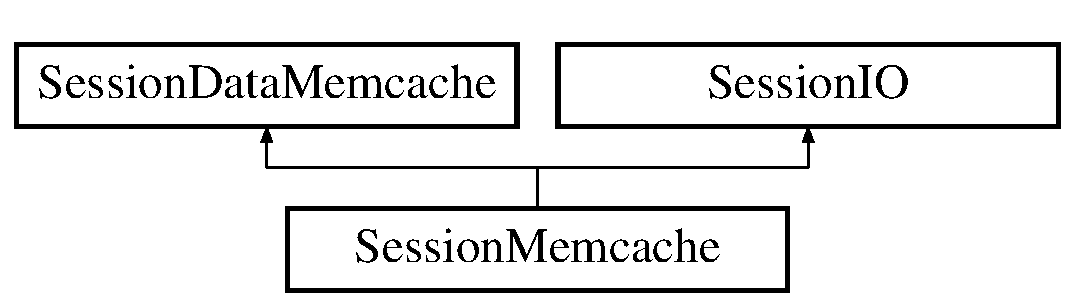
\includegraphics[height=2.000000cm]{class_session_memcache}
\end{center}
\end{figure}
\subsection*{静的公開メンバ関数}
\begin{DoxyCompactItemize}
\item 
static \hyperlink{class_session_memcache_afbae4efe8515a20952293b5aad860470}{set\+Token\+Key} (\$arg\+Token\+Key)
\item 
static \hyperlink{class_session_memcache_a17b8590eb45d4197b1a2aafdd51cb834}{set\+Token\+To\+Cookie} (\$arg\+Token\+Key)
\item 
static \hyperlink{class_session_memcache_ab3f2ecd0f293845de6fb19e3d1618679}{session\+I\+D} (\$arg\+Identifier=N\+U\+L\+L)
\item 
static \hyperlink{class_session_memcache_aa0825e48d7080884156f4d7f91a15c89}{start} (\$arg\+Domain=N\+U\+L\+L, \$arg\+Expiredtime=N\+U\+L\+L, \$arg\+D\+S\+N=N\+U\+L\+L)
\item 
static \hyperlink{class_session_memcache_acde5d140c72c0d5b4738e989fd0e9b66}{get} (\$arg\+Key=N\+U\+L\+L)
\item 
static \hyperlink{class_session_memcache_af6c394389bb0e91f214a985062c2098c}{set} (\$arg\+Key, \$argment)
\item 
\hypertarget{class_session_memcache_a926f82a655e4bb974d7a41291b580f56}{}static {\bfseries clear} ()\label{class_session_memcache_a926f82a655e4bb974d7a41291b580f56}

\end{DoxyCompactItemize}
\subsection*{静的限定公開メンバ関数}
\begin{DoxyCompactItemize}
\item 
static \hyperlink{class_session_memcache_a839fb6db0500fac5d5f23013e19c639d}{\+\_\+init} (\$arg\+Domain=N\+U\+L\+L, \$arg\+Expiredtime=N\+U\+L\+L, \$arg\+D\+S\+N=N\+U\+L\+L)
\item 
static \hyperlink{class_session_memcache_ad3c8b5a5b44b9d986e7b114c436315f8}{\+\_\+token\+To\+Identifier} (\$arg\+Token, \$arg\+Uncheck=F\+A\+L\+S\+E)
\item 
static \hyperlink{class_session_memcache_a33e8d01478a704ea3fe13a2b9518f36e}{\+\_\+identifier\+To\+Token} (\$arg\+Identifier)
\item 
static \hyperlink{class_session_memcache_a275f5f659d2fe68d2daa188ef77eb7b9}{\+\_\+initialize\+Token} ()
\end{DoxyCompactItemize}
\subsection*{静的限定公開変数類}
\begin{DoxyCompactItemize}
\item 
\hypertarget{class_session_memcache_a22c508eebb92819de88e7d2ff9043334}{}static {\bfseries \$\+\_\+\+D\+S\+N} = N\+U\+L\+L\label{class_session_memcache_a22c508eebb92819de88e7d2ff9043334}

\item 
\hypertarget{class_session_memcache_ab14d964e3b8eaa5d3bf6514979503255}{}static {\bfseries \$\+\_\+initialized} = F\+A\+L\+S\+E\label{class_session_memcache_ab14d964e3b8eaa5d3bf6514979503255}

\item 
\hypertarget{class_session_memcache_ab0f11fd3b7f4510cc6874eca70542afb}{}static {\bfseries \$\+\_\+token\+Initialized} = F\+A\+L\+S\+E\label{class_session_memcache_ab0f11fd3b7f4510cc6874eca70542afb}

\item 
\hypertarget{class_session_memcache_a18e1849b0bbffae419bd711abf10efd0}{}static {\bfseries \$\+\_\+replaced} = F\+A\+L\+S\+E\label{class_session_memcache_a18e1849b0bbffae419bd711abf10efd0}

\item 
\hypertarget{class_session_memcache_a4c52dea29245a313eb8aa0e7fddb0927}{}static {\bfseries \$\+\_\+token\+Key\+Name} = \textquotesingle{}token\textquotesingle{}\label{class_session_memcache_a4c52dea29245a313eb8aa0e7fddb0927}

\item 
\hypertarget{class_session_memcache_adc49037c730a5540b6a7620e7e94773e}{}static {\bfseries \$\+\_\+token} = N\+U\+L\+L\label{class_session_memcache_adc49037c730a5540b6a7620e7e94773e}

\item 
\hypertarget{class_session_memcache_a87f6d71c3d3cd0f3fac4cbf6da484c87}{}static {\bfseries \$\+\_\+identifier} = N\+U\+L\+L\label{class_session_memcache_a87f6d71c3d3cd0f3fac4cbf6da484c87}

\item 
\hypertarget{class_session_memcache_ae3ac0a713a449d22aa3e5a09af576515}{}static {\bfseries \$\+\_\+domain} = N\+U\+L\+L\label{class_session_memcache_ae3ac0a713a449d22aa3e5a09af576515}

\item 
\hypertarget{class_session_memcache_aa37f15ed6b6e4dafa05253b06e69d379}{}static {\bfseries \$\+\_\+path} = \textquotesingle{}/\textquotesingle{}\label{class_session_memcache_aa37f15ed6b6e4dafa05253b06e69d379}

\item 
\hypertarget{class_session_memcache_a58a574e235ab48516e50df344ad07d4a}{}static {\bfseries \$\+\_\+expiredtime} = 3600\label{class_session_memcache_a58a574e235ab48516e50df344ad07d4a}

\item 
\hypertarget{class_session_memcache_a5dd5cb5ba2861447803ce4cde3385379}{}static {\bfseries \$\+\_\+session\+Tbl\+Name} = \textquotesingle{}session\+\_\+table\textquotesingle{}\label{class_session_memcache_a5dd5cb5ba2861447803ce4cde3385379}

\item 
\hypertarget{class_session_memcache_a2b9393fcd74a058072fc47a5c3594203}{}static {\bfseries \$\+\_\+session\+P\+Key\+Name} = \textquotesingle{}token\textquotesingle{}\label{class_session_memcache_a2b9393fcd74a058072fc47a5c3594203}

\item 
\hypertarget{class_session_memcache_aabdbeb1bcf3bc5fece544f1eda0ae987}{}static {\bfseries \$\+\_\+session\+Date\+Key\+Name} = \textquotesingle{}create\+\_\+date\textquotesingle{}\label{class_session_memcache_aabdbeb1bcf3bc5fece544f1eda0ae987}

\item 
\hypertarget{class_session_memcache_ae883d74abf717fc163179a54493805b6}{}static {\bfseries \$\+\_\+crypt\+Key} = N\+U\+L\+L\label{class_session_memcache_ae883d74abf717fc163179a54493805b6}

\item 
\hypertarget{class_session_memcache_a10bbda35725655d566951a9c30b4d263}{}static {\bfseries \$\+\_\+crypt\+I\+V} = N\+U\+L\+L\label{class_session_memcache_a10bbda35725655d566951a9c30b4d263}

\end{DoxyCompactItemize}


\subsection{詳解}
Sessionクラス(P\+E\+C\+L\+:Memcache版(非\+P\+E\+C\+L\+:Memcached)) \begin{DoxyAuthor}{著者}
saimushi 
\end{DoxyAuthor}


\subsection{関数詳解}
\hypertarget{class_session_memcache_a33e8d01478a704ea3fe13a2b9518f36e}{}\index{Session\+Memcache@{Session\+Memcache}!\+\_\+identifier\+To\+Token@{\+\_\+identifier\+To\+Token}}
\index{\+\_\+identifier\+To\+Token@{\+\_\+identifier\+To\+Token}!Session\+Memcache@{Session\+Memcache}}
\subsubsection[{\+\_\+identifier\+To\+Token}]{\setlength{\rightskip}{0pt plus 5cm}static Session\+Memcache\+::\+\_\+identifier\+To\+Token (
\begin{DoxyParamCaption}
\item[{}]{\$arg\+Identifier}
\end{DoxyParamCaption}
)\hspace{0.3cm}{\ttfamily [static]}, {\ttfamily [protected]}}\label{class_session_memcache_a33e8d01478a704ea3fe13a2b9518f36e}
固有識別子からトークンを生成する X\+X\+X 各システム毎に、\+Tokenの仕様が違う場合はこのメソッドをオーバーライドして実装を変更して下さい 
\begin{DoxyParams}{引数}
{\em string} & identifier \\
\hline
\end{DoxyParams}
\begin{DoxyReturn}{戻り値}
string token 
\end{DoxyReturn}
\hypertarget{class_session_memcache_a839fb6db0500fac5d5f23013e19c639d}{}\index{Session\+Memcache@{Session\+Memcache}!\+\_\+init@{\+\_\+init}}
\index{\+\_\+init@{\+\_\+init}!Session\+Memcache@{Session\+Memcache}}
\subsubsection[{\+\_\+init}]{\setlength{\rightskip}{0pt plus 5cm}static Session\+Memcache\+::\+\_\+init (
\begin{DoxyParamCaption}
\item[{}]{\$arg\+Domain = {\ttfamily NULL}, }
\item[{}]{\$arg\+Expiredtime = {\ttfamily NULL}, }
\item[{}]{\$arg\+D\+S\+N = {\ttfamily NULL}}
\end{DoxyParamCaption}
)\hspace{0.3cm}{\ttfamily [static]}, {\ttfamily [protected]}}\label{class_session_memcache_a839fb6db0500fac5d5f23013e19c639d}
Sessionクラスの初期化 
\begin{DoxyParams}{引数}
{\em string} & セッションの範囲となるドメイン \\
\hline
{\em string} & セッションの有効期限 \\
\hline
{\em string} & D\+B\+D\+S\+N情報 \\
\hline
\end{DoxyParams}
\hypertarget{class_session_memcache_a275f5f659d2fe68d2daa188ef77eb7b9}{}\index{Session\+Memcache@{Session\+Memcache}!\+\_\+initialize\+Token@{\+\_\+initialize\+Token}}
\index{\+\_\+initialize\+Token@{\+\_\+initialize\+Token}!Session\+Memcache@{Session\+Memcache}}
\subsubsection[{\+\_\+initialize\+Token}]{\setlength{\rightskip}{0pt plus 5cm}static Session\+Memcache\+::\+\_\+initialize\+Token (
\begin{DoxyParamCaption}
{}
\end{DoxyParamCaption}
)\hspace{0.3cm}{\ttfamily [static]}, {\ttfamily [protected]}}\label{class_session_memcache_a275f5f659d2fe68d2daa188ef77eb7b9}
トークンの初期化 \hypertarget{class_session_memcache_ad3c8b5a5b44b9d986e7b114c436315f8}{}\index{Session\+Memcache@{Session\+Memcache}!\+\_\+token\+To\+Identifier@{\+\_\+token\+To\+Identifier}}
\index{\+\_\+token\+To\+Identifier@{\+\_\+token\+To\+Identifier}!Session\+Memcache@{Session\+Memcache}}
\subsubsection[{\+\_\+token\+To\+Identifier}]{\setlength{\rightskip}{0pt plus 5cm}static Session\+Memcache\+::\+\_\+token\+To\+Identifier (
\begin{DoxyParamCaption}
\item[{}]{\$arg\+Token, }
\item[{}]{\$arg\+Uncheck = {\ttfamily FALSE}}
\end{DoxyParamCaption}
)\hspace{0.3cm}{\ttfamily [static]}, {\ttfamily [protected]}}\label{class_session_memcache_ad3c8b5a5b44b9d986e7b114c436315f8}
トークンを固有識別子まで分解する 分解したトークンの有効期限チェックを自動で行います X\+X\+X 各システム毎に、\+Tokenの仕様が違う場合はこのメソッドをオーバーライドして実装を変更して下さい 
\begin{DoxyParams}{引数}
{\em string} & トークン文字列 \\
\hline
\end{DoxyParams}
\begin{DoxyReturn}{戻り値}
mixed パースに失敗したら\+F\+A\+L\+S\+E 成功した場合はstring 固有識別子を返す 
\end{DoxyReturn}
\hypertarget{class_session_memcache_acde5d140c72c0d5b4738e989fd0e9b66}{}\index{Session\+Memcache@{Session\+Memcache}!get@{get}}
\index{get@{get}!Session\+Memcache@{Session\+Memcache}}
\subsubsection[{get}]{\setlength{\rightskip}{0pt plus 5cm}static Session\+Memcache\+::get (
\begin{DoxyParamCaption}
\item[{}]{\$arg\+Key = {\ttfamily NULL}}
\end{DoxyParamCaption}
)\hspace{0.3cm}{\ttfamily [static]}}\label{class_session_memcache_acde5d140c72c0d5b4738e989fd0e9b66}
セッションの指定のキー名で保存されたデータを返す セッションが初期化されていなければ初期化する 
\begin{DoxyParams}{引数}
{\em string} & キー名 \\
\hline
{\em mixed} & 変数全て \\
\hline
\end{DoxyParams}
\hypertarget{class_session_memcache_ab3f2ecd0f293845de6fb19e3d1618679}{}\index{Session\+Memcache@{Session\+Memcache}!session\+I\+D@{session\+I\+D}}
\index{session\+I\+D@{session\+I\+D}!Session\+Memcache@{Session\+Memcache}}
\subsubsection[{session\+I\+D}]{\setlength{\rightskip}{0pt plus 5cm}static Session\+Memcache\+::session\+I\+D (
\begin{DoxyParamCaption}
\item[{}]{\$arg\+Identifier = {\ttfamily NULL}}
\end{DoxyParamCaption}
)\hspace{0.3cm}{\ttfamily [static]}}\label{class_session_memcache_ab3f2ecd0f293845de6fb19e3d1618679}
セッション\+I\+Dを明示的に指定する 
\begin{DoxyParams}{引数}
{\em string} & identifier \\
\hline
\end{DoxyParams}
\hypertarget{class_session_memcache_af6c394389bb0e91f214a985062c2098c}{}\index{Session\+Memcache@{Session\+Memcache}!set@{set}}
\index{set@{set}!Session\+Memcache@{Session\+Memcache}}
\subsubsection[{set}]{\setlength{\rightskip}{0pt plus 5cm}static Session\+Memcache\+::set (
\begin{DoxyParamCaption}
\item[{}]{\$arg\+Key, }
\item[{}]{\$argment}
\end{DoxyParamCaption}
)\hspace{0.3cm}{\ttfamily [static]}}\label{class_session_memcache_af6c394389bb0e91f214a985062c2098c}
セッションに指定のキー名で指定のデータをしまう セッションが初期化されていなければ初期化する 
\begin{DoxyParams}{引数}
{\em string} & キー名 \\
\hline
{\em mixed} & 変数全て(P\+H\+Pオブジェクトは保存出来ない!) \\
\hline
\end{DoxyParams}
\hypertarget{class_session_memcache_afbae4efe8515a20952293b5aad860470}{}\index{Session\+Memcache@{Session\+Memcache}!set\+Token\+Key@{set\+Token\+Key}}
\index{set\+Token\+Key@{set\+Token\+Key}!Session\+Memcache@{Session\+Memcache}}
\subsubsection[{set\+Token\+Key}]{\setlength{\rightskip}{0pt plus 5cm}static Session\+Memcache\+::set\+Token\+Key (
\begin{DoxyParamCaption}
\item[{}]{\$arg\+Token\+Key}
\end{DoxyParamCaption}
)\hspace{0.3cm}{\ttfamily [static]}}\label{class_session_memcache_afbae4efe8515a20952293b5aad860470}
Cookieからトークンを出し入れする時のキー名を変えられるようにする為のアクセサ 
\begin{DoxyParams}{引数}
{\em string} & トークンキー名 \\
\hline
\end{DoxyParams}
\hypertarget{class_session_memcache_a17b8590eb45d4197b1a2aafdd51cb834}{}\index{Session\+Memcache@{Session\+Memcache}!set\+Token\+To\+Cookie@{set\+Token\+To\+Cookie}}
\index{set\+Token\+To\+Cookie@{set\+Token\+To\+Cookie}!Session\+Memcache@{Session\+Memcache}}
\subsubsection[{set\+Token\+To\+Cookie}]{\setlength{\rightskip}{0pt plus 5cm}static Session\+Memcache\+::set\+Token\+To\+Cookie (
\begin{DoxyParamCaption}
\item[{}]{\$arg\+Token\+Key}
\end{DoxyParamCaption}
)\hspace{0.3cm}{\ttfamily [static]}}\label{class_session_memcache_a17b8590eb45d4197b1a2aafdd51cb834}
新しいトークンを指定のトークンキー名で払い出しcookieにセットする 
\begin{DoxyParams}{引数}
{\em string} & トークンキー名 \\
\hline
\end{DoxyParams}
\hypertarget{class_session_memcache_aa0825e48d7080884156f4d7f91a15c89}{}\index{Session\+Memcache@{Session\+Memcache}!start@{start}}
\index{start@{start}!Session\+Memcache@{Session\+Memcache}}
\subsubsection[{start}]{\setlength{\rightskip}{0pt plus 5cm}static Session\+Memcache\+::start (
\begin{DoxyParamCaption}
\item[{}]{\$arg\+Domain = {\ttfamily NULL}, }
\item[{}]{\$arg\+Expiredtime = {\ttfamily NULL}, }
\item[{}]{\$arg\+D\+S\+N = {\ttfamily NULL}}
\end{DoxyParamCaption}
)\hspace{0.3cm}{\ttfamily [static]}}\label{class_session_memcache_aa0825e48d7080884156f4d7f91a15c89}
セッションの開始する(\+\_\+initのアクセサ) 
\begin{DoxyParams}{引数}
{\em string} & セッションの範囲となるドメイン \\
\hline
{\em string} & セッションの有効期限 \\
\hline
{\em string} & D\+B\+D\+S\+N情報 \\
\hline
\end{DoxyParams}

\begin{DoxyExceptions}{例外}
{\em Exception} & \\
\hline
\end{DoxyExceptions}


このクラス詳解は次のファイルから抽出されました\+:\begin{DoxyCompactItemize}
\item 
Framework\+Package/class/\+Session/Session\+Memcache.\+class.\+php\end{DoxyCompactItemize}

\hypertarget{classsimple__html__dom}{}\section{simple\+\_\+html\+\_\+dom クラス}
\label{classsimple__html__dom}\index{simple\+\_\+html\+\_\+dom@{simple\+\_\+html\+\_\+dom}}
simple\+\_\+html\+\_\+dom の継承関係図\begin{figure}[H]
\begin{center}
\leavevmode
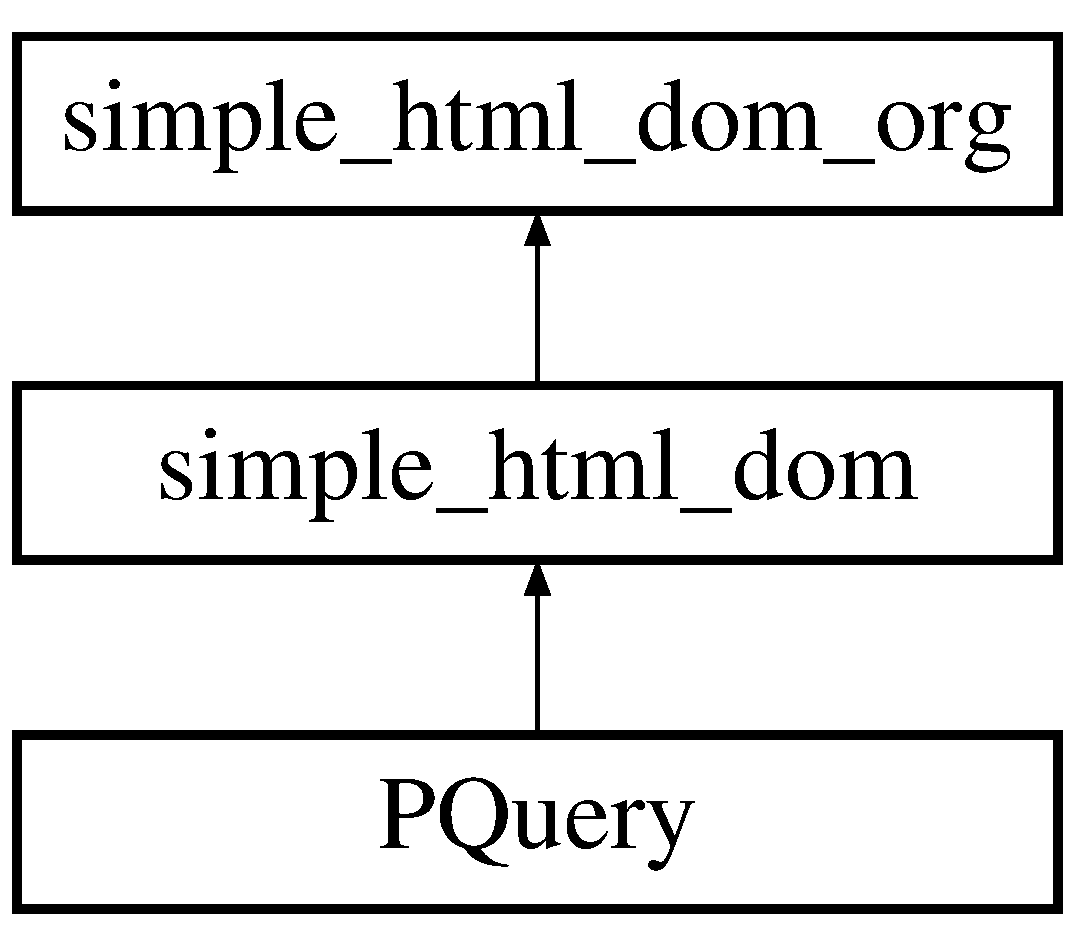
\includegraphics[height=3.000000cm]{classsimple__html__dom}
\end{center}
\end{figure}


このクラス詳解は次のファイルから抽出されました\+:\begin{DoxyCompactItemize}
\item 
Generic\+Package/class/\+Template\+Engine/simple\+\_\+html\+\_\+dom\+\_\+wrapper.\+php\end{DoxyCompactItemize}

\hypertarget{classsimple__html__dom__node}{}\section{simple\+\_\+html\+\_\+dom\+\_\+node クラス}
\label{classsimple__html__dom__node}\index{simple\+\_\+html\+\_\+dom\+\_\+node@{simple\+\_\+html\+\_\+dom\+\_\+node}}
simple\+\_\+html\+\_\+dom\+\_\+node の継承関係図\begin{figure}[H]
\begin{center}
\leavevmode
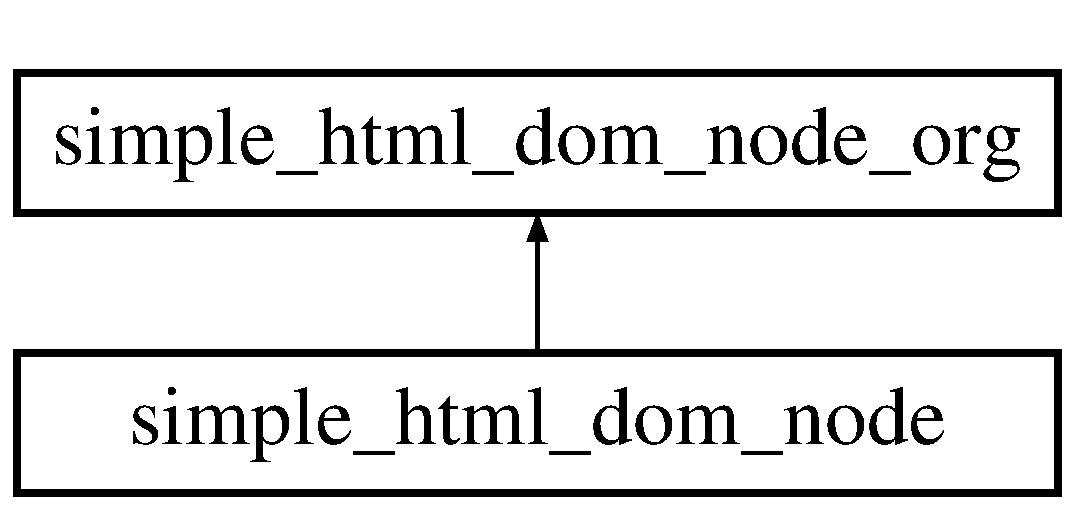
\includegraphics[height=2.000000cm]{classsimple__html__dom__node}
\end{center}
\end{figure}
\subsection*{公開メンバ関数}
\begin{DoxyCompactItemize}
\item 
\hyperlink{classsimple__html__dom__node_a6621f9695c45433db31bef1ddfd1a535}{\+\_\+\+\_\+construct} (\$arg\+D\+O\+M)
\item 
\hyperlink{classsimple__html__dom__node_ace96ee90c681b5c31917f7e9a9919a7f}{innertext} ()
\item 
\hyperlink{classsimple__html__dom__node_a24c24d3a279bbd1ee2e0178769bc06d9}{text\+Nodes} ()
\item 
\hypertarget{classsimple__html__dom__node_a81f75da9128cc4871f5cf8b9d88692e5}{}{\bfseries inner\+Html} (\$arg\+Html\+Text=N\+U\+L\+L)\label{classsimple__html__dom__node_a81f75da9128cc4871f5cf8b9d88692e5}

\item 
\hyperlink{classsimple__html__dom__node_af5120c63522916ee49dafb6a1aaf4b05}{text} (\$arg\+Text=N\+U\+L\+L)
\item 
\hyperlink{classsimple__html__dom__node_a159886a895faf543997faa109c9ff47e}{html} (\$arg\+Html\+Text=N\+U\+L\+L)
\item 
\hyperlink{classsimple__html__dom__node_a967cce7d0454836545657324e19b8330}{remove} ()
\item 
\hyperlink{classsimple__html__dom__node_ab25d8c9e4434dbf6ead41c43dc1d8bca}{flush} ()
\end{DoxyCompactItemize}
\subsection*{公開変数類}
\begin{DoxyCompactItemize}
\item 
\hypertarget{classsimple__html__dom__node_afefb800a237264b8879e9fd537113448}{}{\bfseries \$dom} = N\+U\+L\+L\label{classsimple__html__dom__node_afefb800a237264b8879e9fd537113448}

\end{DoxyCompactItemize}


\subsection{構築子と解体子}
\hypertarget{classsimple__html__dom__node_a6621f9695c45433db31bef1ddfd1a535}{}\index{simple\+\_\+html\+\_\+dom\+\_\+node@{simple\+\_\+html\+\_\+dom\+\_\+node}!\+\_\+\+\_\+construct@{\+\_\+\+\_\+construct}}
\index{\+\_\+\+\_\+construct@{\+\_\+\+\_\+construct}!simple\+\_\+html\+\_\+dom\+\_\+node@{simple\+\_\+html\+\_\+dom\+\_\+node}}
\subsubsection[{\+\_\+\+\_\+construct}]{\setlength{\rightskip}{0pt plus 5cm}simple\+\_\+html\+\_\+dom\+\_\+node\+::\+\_\+\+\_\+construct (
\begin{DoxyParamCaption}
\item[{}]{\$arg\+D\+O\+M}
\end{DoxyParamCaption}
)}\label{classsimple__html__dom__node_a6621f9695c45433db31bef1ddfd1a535}
domを上位クラスでも参照出来るようにコンストラクタをオーバーライド 

\subsection{関数詳解}
\hypertarget{classsimple__html__dom__node_ab25d8c9e4434dbf6ead41c43dc1d8bca}{}\index{simple\+\_\+html\+\_\+dom\+\_\+node@{simple\+\_\+html\+\_\+dom\+\_\+node}!flush@{flush}}
\index{flush@{flush}!simple\+\_\+html\+\_\+dom\+\_\+node@{simple\+\_\+html\+\_\+dom\+\_\+node}}
\subsubsection[{flush}]{\setlength{\rightskip}{0pt plus 5cm}simple\+\_\+html\+\_\+dom\+\_\+node\+::flush (
\begin{DoxyParamCaption}
{}
\end{DoxyParamCaption}
)}\label{classsimple__html__dom__node_ab25d8c9e4434dbf6ead41c43dc1d8bca}
html文字列にして返却 \hypertarget{classsimple__html__dom__node_a159886a895faf543997faa109c9ff47e}{}\index{simple\+\_\+html\+\_\+dom\+\_\+node@{simple\+\_\+html\+\_\+dom\+\_\+node}!html@{html}}
\index{html@{html}!simple\+\_\+html\+\_\+dom\+\_\+node@{simple\+\_\+html\+\_\+dom\+\_\+node}}
\subsubsection[{html}]{\setlength{\rightskip}{0pt plus 5cm}simple\+\_\+html\+\_\+dom\+\_\+node\+::html (
\begin{DoxyParamCaption}
\item[{}]{\$arg\+Html\+Text = {\ttfamily NULL}}
\end{DoxyParamCaption}
)}\label{classsimple__html__dom__node_a159886a895faf543997faa109c9ff47e}
j\+Queryを真似したアクセサ兼セッター \hypertarget{classsimple__html__dom__node_ace96ee90c681b5c31917f7e9a9919a7f}{}\index{simple\+\_\+html\+\_\+dom\+\_\+node@{simple\+\_\+html\+\_\+dom\+\_\+node}!innertext@{innertext}}
\index{innertext@{innertext}!simple\+\_\+html\+\_\+dom\+\_\+node@{simple\+\_\+html\+\_\+dom\+\_\+node}}
\subsubsection[{innertext}]{\setlength{\rightskip}{0pt plus 5cm}simple\+\_\+html\+\_\+dom\+\_\+node\+::innertext (
\begin{DoxyParamCaption}
{}
\end{DoxyParamCaption}
)}\label{classsimple__html__dom__node_ace96ee90c681b5c31917f7e9a9919a7f}
\#0001の為にメソッドをオーバーライド \hypertarget{classsimple__html__dom__node_a967cce7d0454836545657324e19b8330}{}\index{simple\+\_\+html\+\_\+dom\+\_\+node@{simple\+\_\+html\+\_\+dom\+\_\+node}!remove@{remove}}
\index{remove@{remove}!simple\+\_\+html\+\_\+dom\+\_\+node@{simple\+\_\+html\+\_\+dom\+\_\+node}}
\subsubsection[{remove}]{\setlength{\rightskip}{0pt plus 5cm}simple\+\_\+html\+\_\+dom\+\_\+node\+::remove (
\begin{DoxyParamCaption}
{}
\end{DoxyParamCaption}
)}\label{classsimple__html__dom__node_a967cce7d0454836545657324e19b8330}
カラにする \hypertarget{classsimple__html__dom__node_af5120c63522916ee49dafb6a1aaf4b05}{}\index{simple\+\_\+html\+\_\+dom\+\_\+node@{simple\+\_\+html\+\_\+dom\+\_\+node}!text@{text}}
\index{text@{text}!simple\+\_\+html\+\_\+dom\+\_\+node@{simple\+\_\+html\+\_\+dom\+\_\+node}}
\subsubsection[{text}]{\setlength{\rightskip}{0pt plus 5cm}simple\+\_\+html\+\_\+dom\+\_\+node\+::text (
\begin{DoxyParamCaption}
\item[{}]{\$arg\+Text = {\ttfamily NULL}}
\end{DoxyParamCaption}
)}\label{classsimple__html__dom__node_af5120c63522916ee49dafb6a1aaf4b05}
j\+Queryを真似したアクセサ兼セッター \hypertarget{classsimple__html__dom__node_a24c24d3a279bbd1ee2e0178769bc06d9}{}\index{simple\+\_\+html\+\_\+dom\+\_\+node@{simple\+\_\+html\+\_\+dom\+\_\+node}!text\+Nodes@{text\+Nodes}}
\index{text\+Nodes@{text\+Nodes}!simple\+\_\+html\+\_\+dom\+\_\+node@{simple\+\_\+html\+\_\+dom\+\_\+node}}
\subsubsection[{text\+Nodes}]{\setlength{\rightskip}{0pt plus 5cm}simple\+\_\+html\+\_\+dom\+\_\+node\+::text\+Nodes (
\begin{DoxyParamCaption}
{}
\end{DoxyParamCaption}
)}\label{classsimple__html__dom__node_a24c24d3a279bbd1ee2e0178769bc06d9}
タグでくくられていない、テキストノードだけを抽出する 

このクラス詳解は次のファイルから抽出されました\+:\begin{DoxyCompactItemize}
\item 
Generic\+Package/class/\+Template\+Engine/simple\+\_\+html\+\_\+dom\+\_\+wrapper.\+php\end{DoxyCompactItemize}

\hypertarget{class_web_controller_base}{}\section{Web\+Controller\+Base クラス}
\label{class_web_controller_base}\index{Web\+Controller\+Base@{Web\+Controller\+Base}}
Web\+Controller\+Base の継承関係図\begin{figure}[H]
\begin{center}
\leavevmode
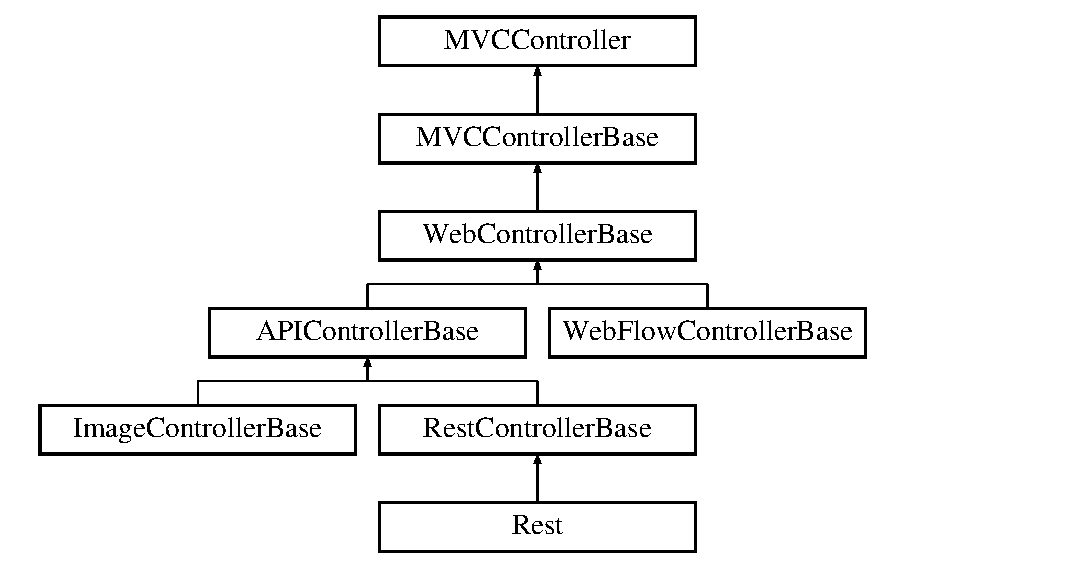
\includegraphics[height=6.000000cm]{class_web_controller_base}
\end{center}
\end{figure}
\subsection*{公開変数類}
\begin{DoxyCompactItemize}
\item 
\hypertarget{class_web_controller_base_aa76c4fb55244a81dd4d15def490aad52}{}{\bfseries \$http\+Status} = 200\label{class_web_controller_base_aa76c4fb55244a81dd4d15def490aad52}

\item 
\hypertarget{class_web_controller_base_aa2e21eaa2c9dcf86a2ea70af99400636}{}{\bfseries \$output\+Type} = \char`\"{}html\char`\"{}\label{class_web_controller_base_aa2e21eaa2c9dcf86a2ea70af99400636}

\end{DoxyCompactItemize}
\subsection*{静的限定公開メンバ関数}
\begin{DoxyCompactItemize}
\item 
\hypertarget{class_web_controller_base_a950063303910b8909b697f3faec17700}{}static {\bfseries \+\_\+clear\+Cache\+Image} (\$arg\+File\+Path, \$arg\+Memcache\+D\+S\+N=N\+U\+L\+L)\label{class_web_controller_base_a950063303910b8909b697f3faec17700}

\end{DoxyCompactItemize}
\subsection*{その他の継承メンバ}


このクラス詳解は次のファイルから抽出されました\+:\begin{DoxyCompactItemize}
\item 
Framework\+Package/class/\+M\+V\+C/Web\+Controller\+Base.\+class.\+php\end{DoxyCompactItemize}

\hypertarget{class_web_flow_controller_base}{}\section{Web\+Flow\+Controller\+Base クラス}
\label{class_web_flow_controller_base}\index{Web\+Flow\+Controller\+Base@{Web\+Flow\+Controller\+Base}}
Web\+Flow\+Controller\+Base の継承関係図\begin{figure}[H]
\begin{center}
\leavevmode
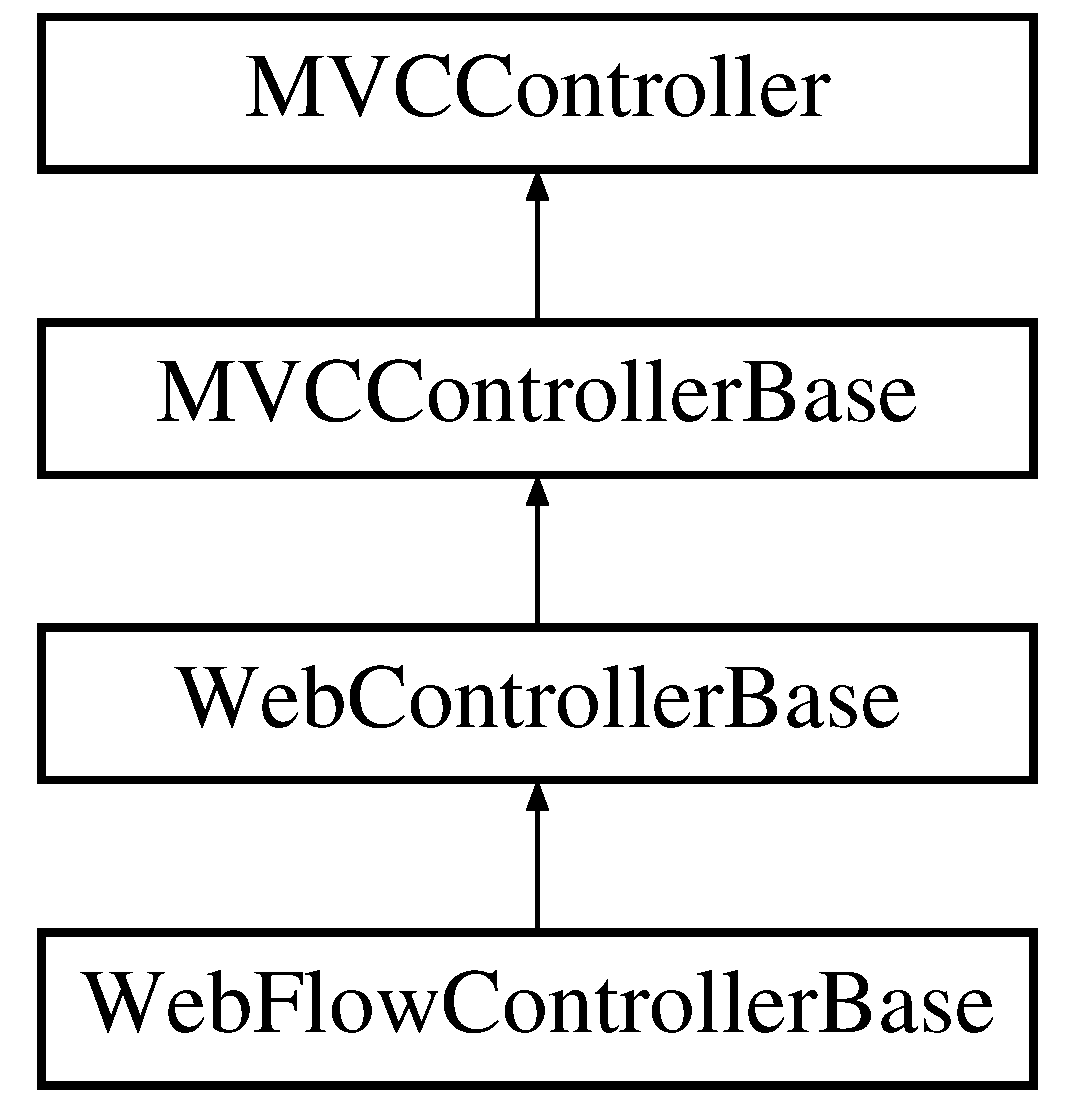
\includegraphics[height=4.000000cm]{class_web_flow_controller_base}
\end{center}
\end{figure}
\subsection*{公開変数類}
\begin{DoxyCompactItemize}
\item 
\hypertarget{class_web_flow_controller_base_a7a24ae7bea03734fd2ca58d7a6a57a9d}{}{\bfseries \$action} =\textquotesingle{}\textquotesingle{}\label{class_web_flow_controller_base_a7a24ae7bea03734fd2ca58d7a6a57a9d}

\item 
\hypertarget{class_web_flow_controller_base_abfa9c5257034cc831f7049ffa31fb9d4}{}{\bfseries \$section} =\textquotesingle{}\textquotesingle{}\label{class_web_flow_controller_base_abfa9c5257034cc831f7049ffa31fb9d4}

\item 
\hypertarget{class_web_flow_controller_base_ac471f8b92614047d421b39d30792df28}{}{\bfseries \$target} =\textquotesingle{}\textquotesingle{}\label{class_web_flow_controller_base_ac471f8b92614047d421b39d30792df28}

\end{DoxyCompactItemize}
\subsection*{静的公開変数類}
\begin{DoxyCompactItemize}
\item 
\hypertarget{class_web_flow_controller_base_a5c29cc9ecd2e29c39f7412c71fe28820}{}static {\bfseries \$flowpostformsection\+Used} = F\+A\+L\+S\+E\label{class_web_flow_controller_base_a5c29cc9ecd2e29c39f7412c71fe28820}

\end{DoxyCompactItemize}
\subsection*{限定公開メンバ関数}
\begin{DoxyCompactItemize}
\item 
\hypertarget{class_web_flow_controller_base_ab9f557b84cee49999a493996431c3087}{}{\bfseries \+\_\+reverse\+Rewrite\+U\+R\+L} (\$arg\+Action=N\+U\+L\+L, \$arg\+Query=\textquotesingle{}\textquotesingle{})\label{class_web_flow_controller_base_ab9f557b84cee49999a493996431c3087}

\item 
\hypertarget{class_web_flow_controller_base_ac502f82273a95f57d7ddb0311533b1ac}{}{\bfseries \+\_\+init\+Web\+Flow} ()\label{class_web_flow_controller_base_ac502f82273a95f57d7ddb0311533b1ac}

\end{DoxyCompactItemize}
\subsection*{その他の継承メンバ}


このクラス詳解は次のファイルから抽出されました\+:\begin{DoxyCompactItemize}
\item 
Framework\+Package/class/\+Flow/Web\+Flow\+Controller\+Base.\+class.\+php\end{DoxyCompactItemize}

%--- End generated contents ---

% Index
\backmatter
\newpage
\phantomsection
\clearemptydoublepage
\addcontentsline{toc}{chapter}{索引}
\printindex

\end{document}
